\documentclass[11pt]{article}

% ---------------------------------------------------------------------------
% Layout
% ---------------------------------------------------------------------------
\usepackage[margin=1in]{geometry}
\usepackage{setspace}
\onehalfspacing
\usepackage[T1]{fontenc}
\usepackage{lmodern}
\usepackage{microtype}

% ---------------------------------------------------------------------------
% Mathematics
% ---------------------------------------------------------------------------
\usepackage{amsmath,amssymb,mathtools,bm}
\usepackage{algorithm}
\usepackage{algpseudocode}

% ---------------------------------------------------------------------------
% Tables and figures
% ---------------------------------------------------------------------------
\usepackage{booktabs,threeparttable,tabularx,longtable,multirow,makecell}
\usepackage{graphicx}
\usepackage{xcolor}
\usepackage{tikz}
\usetikzlibrary{arrows.meta,positioning,shapes.geometric,fit,calc,backgrounds}
\usepackage{caption}
\usepackage{subcaption}
\usepackage{float}
\usepackage{placeins}
\usepackage{pdflscape}
\usepackage{siunitx}
\usepackage{enumitem}
\captionsetup{font=small,labelfont=bf,justification=justified,singlelinecheck=false}
\graphicspath{{figures/}}

% Palette shared with scripts/paper/_paper_theme.R so diagrams match the plots.
\definecolor{osiblue}{HTML}{2A78D6}
\definecolor{osiorange}{HTML}{EB6834}
\definecolor{osiaqua}{HTML}{1BAF7A}
\definecolor{osiyellow}{HTML}{EDA100}
\definecolor{osiviolet}{HTML}{4A3AA7}
\definecolor{osigray}{HTML}{898781}
\definecolor{osilight}{HTML}{F0EFEC}
\definecolor{osiink}{HTML}{0B0B0B}

% ---------------------------------------------------------------------------
% Bibliography and links
% ---------------------------------------------------------------------------
\usepackage[authoryear,round]{natbib}
\bibliographystyle{aer}
\usepackage[hidelinks]{hyperref}
\usepackage[title]{appendix}

% ---------------------------------------------------------------------------
% Notation (defined once; see Section~\ref{sec:framework})
% ---------------------------------------------------------------------------
% Indices: i country, j partner, t technology, s supply-chain stage,
% k category, v variable.
\newcommand{\Countries}{\mathcal{I}}
\newcommand{\Techs}{\mathcal{T}}
\newcommand{\Stages}{\mathcal{S}}
\newcommand{\Cats}{\mathcal{K}}
\newcommand{\Coalition}{\mathcal{N}}
\newcommand{\cell}{(i,t,s)}
\newcommand{\dyad}{(i,j,t,s)}
\newcommand{\Scurve}{\phi_{\gamma}}
\newcommand{\ES}{\mathrm{ES}}
\newcommand{\EO}{\mathrm{EO}}
\newcommand{\POL}{\mathrm{POL}}
% siunitx defines \SI (number + unit); the paper never uses that form, so the name is
% taken for the Strategic Index. Use \qty{}{} if a quantity with units is ever needed.
\renewcommand{\SI}{\mathrm{SI}}
\newcommand{\FS}{\mathrm{FS}}
\newcommand{\PO}{\mathrm{PO}}
\newcommand{\DP}{\mathrm{DP}}
\newcommand{\PSI}{\mathrm{PSI}}
\newcommand{\HHI}{\mathrm{HHI}}
\newcommand{\RCA}{\mathrm{RCA}}
\newcommand{\1}{\mathbf{1}}
\DeclareMathOperator*{\argmax}{arg\,max}
\DeclareMathOperator{\rank}{rank}
\DeclareMathOperator{\mean}{mean}

% Online Appendix numbering: sections OA.1, OA.2, ...; floats and equations OA.n.
\newcommand{\startonlineappendix}{%
  \clearpage
  \setcounter{section}{0}\setcounter{figure}{0}\setcounter{table}{0}%
  \setcounter{equation}{0}\setcounter{algorithm}{0}%
  \renewcommand{\thesection}{OA.\arabic{section}}%
  \renewcommand{\thesubsection}{\thesection.\arabic{subsection}}%
  \renewcommand{\thefigure}{OA.\arabic{figure}}%
  \renewcommand{\thetable}{OA.\arabic{table}}%
  \renewcommand{\theequation}{OA.\arabic{equation}}%
  \renewcommand{\thealgorithm}{OA.\arabic{algorithm}}%
  \renewcommand{\theHsection}{OA.\arabic{section}}%
  \renewcommand{\theHsubsection}{\theHsection.\arabic{subsection}}%
  \renewcommand{\theHfigure}{OA.\arabic{figure}}%
  \renewcommand{\theHtable}{OA.\arabic{table}}%
  \renewcommand{\theHequation}{OA.\arabic{equation}}%
  \renewcommand{\theHalgorithm}{OA.\arabic{algorithm}}%
  \phantomsection\pdfbookmark[0]{Online Appendix}{onlineappendix}%
  \begin{center}
    {\LARGE\bfseries Online Appendix\par}\vspace{6pt}
    {\large Opportunity, Security, and the Allied Industrial Base\par}\vspace{4pt}
    {\normalsize Further detail, derivations and diagnostics\par}
  \end{center}
  \vspace{12pt}}

% ---------------------------------------------------------------------------
\title{Opportunity, Security, and the Allied Industrial Base:\\
A Quantitative Network Approach to Coalition Supply Chains for Energy Technologies}

\author{[Author names]\thanks{RMI. [Contact details and acknowledgements.] The
indices, code and replication materials are produced by the Opportunity
Security Indices pipeline; every number in this paper is generated by the
scripts in \texttt{scripts/paper/}.}}

\date{October 2026}

\begin{document}

\maketitle

% ---------------------------------------------------------------------------
% Abstract (input by main.tex after \maketitle; no preamble).
% Numbers: final rerun of 2026-10-12 (paper/results/*.json): network.json (China leads 10 of 18
% basket stages; median designed HHI 0.1520; share of production outside the three largest
% exporting nodes, median stage 0.6625; non-high-income Upstream share 0.465), strategic.json and
% robustness.json (27 Batteries Midstream picks; 21 of 57 margins below 0.01), method.json.
% ---------------------------------------------------------------------------
\begin{abstract}
\noindent No allied economy can efficiently reproduce the whole supply chain of energy
technologies, so protection against concentrated suppliers must come from allocating
capabilities across trusted partners: managed interdependence rather than autarky. We build a
framework to measure and design it. Energy-security and economic-opportunity pillars
score 219 economies in up to 33 technology--stage cells. A Strategic Index reads security as need,
and an endowment screen admits extraction stages to a member's priority only where it has a
resource base. A 57-member coalition (37 network
nodes) is derived from UN General Assembly ideal points, agreements and world supply shares.
Bilateral indices rate partners as suppliers and markets, and a mixed-integer program allocates
production in 22 upstream and midstream stages under a diversification penalty calibrated to
observed export concentration. China is the largest exporter in 10 of the 18 traded stages. The
calibrated design spreads each stage over seven to ten producers (median Herfindahl index 0.152)
and, because it scores capability rather than current capacity, places two-thirds of the median
stage's production outside today's three largest exporting nodes and 47 percent of upstream output
in non-high-income members. Battery midstream is the most common national priority (27 members),
far more than the nine producers the network design assigns it, and 21 of the 57 priorities lie
within 0.01 of the runner-up. The
framework turns rankings into an auditable division of labour.
\end{abstract}

\medskip
\noindent\textbf{JEL codes:} C43, C61, F14, F52, L52, Q48.

\noindent\textbf{Keywords:} allied industrial base; energy security; economic opportunity;
composite indicators; friend-shoring; geopolitical alignment; supply-chain network design;
industrial policy.


\newpage

% ---------------------------------------------------------------------------
% Section 1: Introduction (input by main.tex; no preamble).
% Framing: the NEIS working paper on the Allied Industrial Base (neis2026allied; text in
% integration/aib_concept_review.md), paraphrased and cited, not copied.
% Numbers: final rerun of 2026-10-12, read from paper/results/*.json (method, es, eo, joint,
% coalition, strategic, bilateral, aib, aib_robustness, robustness).
% ---------------------------------------------------------------------------
\section{Introduction}\label{sec:intro}

Energy security used to be a matter of fuels: reserves, import routes and stocks of oil and gas.
As solar panels, batteries, grids and power electronics absorb a growing share of energy
investment, it is increasingly a matter of manufactured systems and of the minerals and components
they are made from \citep{carey2025secure, iea2024etp}. A country can now be secure in fuels and
exposed in transformers, battery materials or magnets. These manufacturing chains are
concentrated. In the trade data used in this paper, China is the largest world exporter in nine of
the 18 upstream and midstream technology--stage baskets that have a product definition, with
shares between 19 and 44 percent, and the refining of rare earths and the manufacture of magnets
and battery anode material are concentrated in China at shares close to or above 90 percent
\citep{iea2025gcmo, iea2026etp}. Concentration is not in itself a market failure; it reflects
scale economies, learning and geology. But it determines how far a disruption travels through
production networks \citep{acemoglu2012network, carvalho2021supply, baqaee2019macroeconomic},
and it turns trade into leverage. \citet{hirschman1945national} made the point for bilateral trade
dependence, and \citet{farrell2019weaponized} show that states with jurisdiction over the central
nodes of global networks can observe, restrict or deny access to them.

The response so far has been national. Governments have returned to industrial policy on a scale
not seen for decades \citep{juhasz2024new, evenett2024return}, often with sourcing rules that tie
subsidies to where minerals are processed and components made \citep{bown2023industrial}. National
programmes are meeting economic and political limits. Several economies have targeted the same
manufacturing segments without the demand or cost position to fill the plants, and announced
capacity has been cancelled as prices fell \citep{iea2026etp}; subsidy competition reaches allies
\citep{clausing2023carbon}; and tighter public finances make it implausible for every large
economy to fund a complete green-industrial agenda \citep{ladislaw2025evolution}. Smaller
economies cannot replicate the demand-led strategies of the largest ones at all
\citep{albertone2025regional}. Autarky is the expensive alternative. Simulations of broad
relocalisation find large losses of trade and output without consistent gains in resilience, and
diversification usually does more for resilience than reshoring \citep{oecd2025supply,
thakurweigold2024promoting}. Deep fragmentation into blocs is costly too, most of all for small
economies \citep{aiyar2023geoeconomic, javorcik2024economic}.

These observations underpin the proposition of an Allied Industrial Base
\citep{campbell2025underestimating, neis2026allied}. Matching China's scale across the
electro-industrial supply chains is beyond any one allied economy. The premise is that allied
economies jointly hold the markets, capital, resources and know-how that none holds alone, but
deploy them through competing national strategies \citep{campbell2025underestimating,
neis2026allied}. The working paper accordingly frames the policy goal as \emph{managed
interdependence}: each strategically important capability should be available at scale from some
trusted member, with redundancy where a failure would be very costly, specialisation where scale
economies and learning dominate, and open global sourcing where the risk is small
\citep{neis2026allied}. Implementing it requires answers to questions
that the literature mostly leaves open: which nodes of
which supply chains are severe enough to coordinate, who counts as a trusted partner, and which
member should produce what \citep[Section 5]{neis2026allied}.

This paper asks how a coalition of economies could allocate energy-technology supply chains
among its members, technology by technology and stage by stage, and builds the measurements that
such an allocation needs. The unit of analysis is a cell $\cell$: an economy, one of eleven
technologies (batteries, coal, electric grid, electric vehicles, gas, geothermal, green hydrogen,
nuclear, oil, solar and wind) and one of three stages (upstream extraction, midstream processing
and manufacturing, downstream deployment). Two pillars score the cells of 219 economies: Energy
Security ($\ES$), how secure an economy's supply is, and Economic Opportunity ($\EO$), how well
placed it is to compete as a producer. Both are built from rank-based S-curves of public data,
among them the IEA, the Energy Institute, the U.S. Geological Survey, UN Comtrade and the Atlas
of Economic Complexity (Section~\ref{sec:data}), and a cell
enters a ranking only if the economy is sovereign and observed data carry at least half of its
weight. A Strategic Index combines the pillars with a policy index into a within-country ranking
of sectors in which security enters as \emph{need}, favouring sectors where a country is exposed
but capable; an endowment screen keeps an extraction stage out of a member's priority unless the
member has the resource. The coalition is derived rather than chosen: from ideal points estimated
from UN General Assembly votes \citep{bailey2017estimating}, membership of U.S. trade and security
agreements, and shares of world supply. It has 31 core members on the U.S.-leaning side of the
Assembly with GDP of at least USD 100 billion and 26 partners admitted through agreements or as
major suppliers. Bilateral indices
score each partner as a friendshoring opportunity, where an economy's security need in a sector
meets the partner's economic opportunity on existing trade and investment ties, and as an export
market, taking account of alignment and, in four manufacturing stages, of the Chinese ownership of
the partner's foreign-invested plants. Finally,
an Allied Industrial Base analysis stress-tests 92 sub-sector nodes of the observed 2024 trade
network: it removes a dominant supplier, measures how much of the coalition's lost supply existing
relationships and optimized partnerships restore, simulates standardised capacity increments where
a gap remains, and groups the nodes that need joint action into Sectoral Compacts with exact
minimum coalitions. Figure~\ref{fig:framework_architecture}
sets out the architecture.

The paper makes four contributions. The first is measurement at the level of the supply-chain
node. Security and opportunity are scored jointly, on a common scale and with a common variable
architecture, for each stage of each technology; the scores decompose exactly into category and
variable contributions, and a rankability rule keeps cells that rest mostly on imputation out of
every ranking. Existing energy-security indices describe an energy system or a fuel, and
green-complexity measures describe products \citep{mealy2022economic, growthlab2024greenplexity};
neither pairs exposure with capability in the same cell. The second turns the pillars into
priorities while keeping the normative choices visible: the need reading of security, the
endowment screen, the basis of the policy index and the margin of each member's priority over its
runner-up are reported with the results. The third is a rule-based coalition and bilateral layer.
Alignment is measured from Assembly votes rather than asserted, the coalition and its tiers
follow from stated thresholds, and the bilateral indices carry both alignment and a first measure
of the common-mode risk that arises when suppliers in different countries share Chinese parents.
The fourth is a stress test of the allied supply network at the level of the sub-sector. It
separates the economies protected from those that may supply them, distinguishes what existing
relationships, coordinated trade and new capacity each contribute, checks trade-based capability
against physical production data where they exist, and forms Sectoral Compacts only where chains,
partners and policy needs cohere, with coalitions found by an exact binary program rather than by
ranking. It answers the working paper's question of where coordination pays \citep{neis2026allied}
with a measured coordination dividend, and it reports no composite score. The pipeline is open and configuration-driven, and the
corrections made during an end-to-end audit of an earlier version are documented in
Appendix~\ref{app:corrections}.

Five sets of results stand out. First, the coalition is stronger on security than on opportunity.
A coalition member leads 16 of the 30 security pairs and is in the top three of all 30, but the
best-placed member leads only 8 of the 33 opportunity pairs, against 22 for China. The two
pillars are correlated within pairs (median Spearman 0.59), largely through shared components:
on the 23 pairs in which both pillars keep components of their own, the median falls from 0.55
to 0.30 when only the non-shared components are used. About 15 percent of
the cells rankable on both pillars combine above-median opportunity with below-median security,
the region the Strategic Index favours. Second, members' priorities concentrate on manufacturing.
The index scores 3,154 cells in 174 countries, and every one of the 57 members has an allied
pick: 43 are midstream, and battery midstream alone is the pick of 27. The endowment screen
changes 41 picks, mostly away from upstream stages in which a member has a need but no resource.
The picks are fragile: the median margin over the runner-up is 0.015, 21 picks lie within 0.01,
and only five survive if security is read as strength rather than need. Third, alignment shapes
the partnership rankings. Viewed from the 31 core members, the United States and Germany are the
strongest partners and core members hold 24 of the top 25 places; giving the alignment component
zero weight would lift China from 44th to 3rd. Fourth, the allies' exposure is a capacity problem.
With China's supply removed, the 57 members lose 22.9 percent of their traded demand for
electro-industrial goods (47.5 percent in batteries); existing relationships and optimized trade
restore coverage only to 84.7 percent, and all of the recovery, USD 232 billion, is supply drawn
from buyers outside the coalition. New or expanded relationships add less than one point of coverage in
81 of the 91 nodes, and no node is classed as a case for trade coordination: 37 of the 70 electro-industrial nodes
need new capacity, and they form 22 Sectoral Compacts, all of them investment and offtake clubs, whose
exact minimum coalitions have three to nine countries. Fifth, rankings are more robust than
classifications. Country rankings within pairs barely move under random category weights (median
within-pair Spearman 0.997 for security and 0.988 for opportunity), and an empirical test of vertical
complementarities finds no out-of-sample gain from rewarding a stage for capability at adjacent
stages; the AIB classes, by contrast, depend on how the shock is read: if China's purchases fall with
its sales, 24 rather than 37 electro-industrial nodes need new capacity.

The results speak to some open questions of the working paper
\citep[Section 10]{neis2026allied} but not to others. It answers the question of when coordination
pays: against a China shock, rarely through trade alone, since the existing network already carries
nearly all that trade can do, and chiefly through capacity at capable hosts, organised by coalitions
of a few countries. It answers the question of how much duplication is enough only in part: a 25
percent supplier-share limit costs less than two points of coverage against the shock in 77 of the
91 nodes, but where capacity is missing no tested limit restores resilience to a second loss. The paper does not test the hypotheses that allied specialisation reaches a
resilience target at lower public cost than parallel national programmes, that demand coordination matters more than subsidy coordination, or that fencing
nodes dominates excluding sectors: these need cost, revenue and bankability data that the indices
do not contain (Section~\ref{sec:discussion}).

The rest of the paper is organised as follows. Section~\ref{sec:framework} sets out the
conceptual framework and notation and Section~\ref{sec:data} the data.
Section~\ref{sec:normalization} presents the normalisation, imputation and rankability rules.
Sections~\ref{sec:es} and~\ref{sec:eo} construct the Energy Security and Economic Opportunity
pillars, and Section~\ref{sec:joint} studies the joint space they define.
Section~\ref{sec:coalition} measures geopolitical alignment and derives the coalition,
Section~\ref{sec:strategic} builds the Policy and Strategic indices, Section~\ref{sec:bilateral}
the bilateral indices, and Section~\ref{sec:network} the Allied Industrial Base analysis of shocks,
partnerships and Sectoral Compacts.
Section~\ref{sec:robustness} reports robustness analyses, and Section~\ref{sec:discussion}
discusses the results, next steps and limitations.

% ---------------------------------------------------------------------------
\subsection{Related literature}\label{subsec:literature}

The Allied Industrial Base lies where several literatures meet that are usually read separately
\citep{neis2026allied}. We organise them by the streams that bear on its design and then turn to
the measurement literatures on which the indices build.

\paragraph{Industrial policy and capabilities.} \citet{rodrik2004industrial} recast industrial
policy as a process of discovery and strategic collaboration rather than the selection of
winners, and \citet{juhasz2024new} review a new empirical literature that is more favourable to it
while stressing context, measurement and governance; text-based and intervention-level data now
make policy measurable \citep{juhasz2022who, evenett2024return}. The green variant rests on
learning, coordination and environmental externalities \citep{rodrik2014green}, and its current
form ties support to location \citep{bown2023industrial, bistline2023economic}. This literature
studies the relation between a state and its firms. The coordination failures it identifies, such
as uncertain demand, missing suppliers and first-mover costs, do not stop at borders, and the
governance of industrial interdependence among several states remains thinly studied. Our Policy
index records the presence and density of policy by sector; it does not measure effectiveness.

\paragraph{Supply-chain resilience and economic security.} Production-network models show that
shocks to central suppliers need not average out \citep{acemoglu2012network,
carvalho2019production, baqaee2019macroeconomic}, that disruptions propagate along supply chains
\citep{carvalho2021supply}, and that private sourcing decisions can leave networks fragile
\citep{elliott2022supply}. \citet{grossman2023supply} analyse the choice between diversification
and reshoring, and \citet{baldwin2022risks} separate exposure from resilience. Policy work defines
a critical dependency as the combination of high disruption risk, high importance and limited
substitutability \citep{oecd2025economic}, and finds diversification generally more effective
than relocalisation \citep{oecd2025supply, thakurweigold2024promoting}. These results motivate
scoring by stage, separating exposure ($\ES$) from capability ($\EO$), and stress-testing the
allied network node by node. The AIB analysis shocks each node separately and does not model
propagation along the chain, and the bilateral indices capture
direct exposure only, not the indirect dependence that \citet{freund2024us} document.

\paragraph{Weaponized interdependence and allied scale.} \citet{farrell2019weaponized} show how
the hubs of global networks confer coercive power, which shifts attention from national market
shares to network position, a modern form of the concern of \citet{hirschman1945national}.
\citet{campbell2025underestimating} argue that only a coalition can match China's productive
scale and that alliances must pool capacity, not only political support. Friend-shoring
\citep{yellen2022remarks} and the evidence on fragmentation give this argument empirical content:
trade and investment between geopolitical blocs have weakened relative to flows within them
\citep{gopinath2025changing}, U.S. sourcing has moved away from China toward economies that are
themselves integrated with Chinese supply chains \citep{alfaro2023global, freund2024us}, and
confining trade to aligned partners carries welfare costs \citep{goes2022impact,
javorcik2024economic, aiyar2023geoeconomic}.

\paragraph{Regional industrial policy and historical coordination.}
\citet{albertone2025regional} show, for ASEAN, that cross-border industrial strategy must manage
competition as well as cooperation, and that coordination without integration needs mechanisms
that reveal synergies and monitor commitments. Historical cases point the same way. The Combined
Boards of 1942--45 pooled the raw materials and production of the United States, the United
Kingdom and Canada and allocated scarce output against total requirements
\citep{usdos1942combined, uswpb1944war}. Airbus combined national specialisation with shared
demand and public risk-taking \citep{ec2022industrial, imf2024industrial}. The European Coal and
Steel Community placed strategic sectors under common rules \citep{eu1951ecsc}. Each worked
around a concrete objective, clear roles and benefits reciprocal enough to sustain it.

\paragraph{Systemic bankability.} \citet{spokas2025systemic} show that infrastructure
technologies stall when any part of the surrounding system (offtake, permitting, enabling
infrastructure, insurance, supply chains, delivery capacity) is missing, so that a designated
capability is not a capability until it is bankable. Our indices do not measure bankability,
which is the main reason the investment step of the AIB analysis is a capacity simulation rather
than a project pipeline.

\paragraph{Competing schools.} The policy debate divides into three schools
\citep{neis2026allied}. The first defends multilateral openness and stresses the costs of
fragmentation \citep{aiyar2023geoeconomic, oecd2025supply}. The second, closest to the Allied
Industrial Base, accepts selective de-risking within managed interdependence. The third proposes
a reciprocal bloc that conditions market access on balanced obligations and the exclusion of
China \citep{cass2025grand}. Our coalition rule belongs with the second: it admits nonaligned and
even China-leaning economies through agreements or supply shares, and it fences off no sector as
a whole.

\paragraph{Measurement.} Four measurement literatures supply the building blocks. Energy-security
indicators organise availability, dependence, diversity and affordability
\citep{kruyt2009indicators, sovacool2011conceptualizing, ang2015energy, jewell2011iea} and define
security as the low vulnerability of vital systems \citep{cherp2014concept,
winzer2012conceptualizing}; mineral criticality combines supply risk with vulnerability
\citep{graedel2012methodology, nassar2020evaluating, kowalski2023raw}. Most such indices describe
an energy system or a fuel, whereas $\ES$ applies their logic to each stage of each technology.
Economic complexity treats exports as revealing capabilities \citep{balassa1965trade,
hidalgo2007product, hausmann2006structural, hidalgo2009building, hausmann2014atlas}, with
relatedness predicting future specialisation \citep{hausmann2022implied} and applications to
green products \citep{mealy2022economic, growthlab2024greenplexity}; $\EO$ combines these signals
with demand, cost, readiness and investment. The composite-indicator literature disciplines
normalisation, weighting and uncertainty analysis \citep{oecd2008handbook, saisana2005uncertainty,
paruolo2013ratings}, and our S-curve is the probability-weighting function of
\citet{karmarkar1978subjectively}. Alignment is measured with UN-vote ideal points
\citep{bailey2017estimating, voeten2009unga}, in the tradition of foreign-policy similarity
measures \citep{signorino1999taub} and with the bloc definitions of \citet{gopinath2025changing}.
The AIB layer draws on supply-chain network design and disruption-aware sourcing
\citep{geoffrion1974multicommodity, melo2009facility, tomlin2006value, snyder2016orms}, solved as
lexicographic linear programs \citep{ehrgott2005multicriteria}. It departs from that tradition by
restoring observed traded demand under explicit shocks rather than minimising cost, and by treating
the allied network as emergent from bilateral relationships rather than designed.

\paragraph{The gap.} Read together, these literatures diagnose the problem better than they
allocate a response \citep[Section 5]{neis2026allied}: they establish why capabilities and
concentrated dependencies matter, why allied scale can offset national limits and why autarky is
costly, but not who should produce what, or how much duplication suffices. Nor do they offer a
common measurement architecture that connects sector priorities, partner capabilities and
performance. The indices of \citet{carey2025secure} were a
first step. They score eleven technologies across commodities, manufacturing and deployment on
energy-security risk and economic opportunity, read the joint space as four strategic postures,
and rate partners as safer, stronger or more prosperous with weights 0.4, 0.2 and 0.4. This paper
takes them from rankings to a stress test of the allied network. It rebuilds the pillars at the level of the cell with
a rankability rule, derives the coalition from observed alignment and supply, rates every
directed partnership, and adds an analysis of observed trade that shows, node by node, where
existing relationships suffice, where coordination would help, where allies must build and which
countries a compact needs.

% ===========================================================================
% Section 2. Conceptual framework (input by main.tex; no preamble).
% Framing: NEIS working paper on the Allied Industrial Base (neis2026allied): definition, the
% Severity -> Coordination -> Specialization logic and the five analytical layers (its Sections
% 2, 7 and 8), paraphrased and cited.
% Specification (code is the specification): config/weights.yml, config/rankability.yml,
%   R/utils/scurve.R, R/indices/index_builder_core.R, R/indices/build_policy_index.R,
%   R/indices/build_indices.R (Strategic Index, endowment screen, allied pick),
%   R/geopolitical_distance/*.R and scripts/12 (alignment), R/indices/coalition.R and scripts/13
%   (tiers, EU node), R/themes/partnership_strength/*.R (FS, PO, DP, PSI),
%   R/indices/allied_network_design.R and scripts/30 (network; lambda = 0.78, node policy term off).
% Figure fig:framework_architecture is drawn inline (TikZ) so that it matches the final method.
% ===========================================================================
\section{Conceptual framework}\label{sec:framework}

This section places the paper within the analytical architecture proposed for an Allied
Industrial Base \citep{neis2026allied}, states which parts of that architecture the paper
measures and which it leaves aside, and then defines the objects used in the rest of the paper.
Figure~\ref{fig:framework_architecture} summarises the construction and Table~\ref{tab:notation}
collects the notation.

% ---------------------------------------------------------------------------
\subsection{The allied industrial base as a design problem}\label{subsec:framework_aib}

The working paper defines an Allied Industrial Base by its purpose: trusted economies coordinate
strategically important capabilities so that, together, they reach a resilience and scale that
none could reach efficiently alone \citep{neis2026allied}. The object is
the network: a capability should exist at sufficient scale somewhere among trusted partners, not
in every member. The unit of policy is the \emph{node}, a step such as mineral refining or
component manufacture, because one supply chain can warrant different treatment at different
steps. And the problem is one of allocation: which capabilities should be domestic, duplicated,
specialised among partners or left to global markets.

The working paper orders the decision in three steps. \emph{Severity} asks how damaging a
disruption would be and how hard substitution or recovery would be; \emph{coordination}, whether
the problem needs international action rather than private diversification or national policy;
and \emph{specialization}, where the capability should reside and what should be duplicated. The
evidence is organised in five analytical layers: node criticality and severity, country
capability and opportunity, partner complementarity and reciprocity, systemic bankability, and
network robustness under stress. The object is a combination of capabilities, not a ranking: a
partner that ranks low in isolation can be indispensable if it supplies what the network lacks.

Table~\ref{tab:framework_layers} maps the layers onto this paper. We measure each economy's
relative exposure within a node by the need term $1-\ES$ (rank-based, so it does not compare
severity across nodes) and, for extraction, apply the endowment screen; capability by
$\EO$, with the Policy index recording where governments already concentrate their effort;
complementarity, alignment and part of reciprocity by the coalition and the bilateral indices;
and robustness only in part, by the diversification penalty and multi-sourcing constraints of the
network design. Systemic bankability \citep{spokas2025systemic}, common-mode risk (beyond a first
measure of the Chinese ownership of suppliers' foreign-invested plants), dynamic option value,
reciprocal obligations, resilience floors and stress tests are not modelled.

\begin{table}[tbp]
\centering
\begin{threeparttable}
\caption{The analytical layers of an Allied Industrial Base and their counterparts in this paper}
\label{tab:framework_layers}
\footnotesize
\begin{tabularx}{\textwidth}{@{}>{\raggedright\arraybackslash}p{2.7cm}
  >{\raggedright\arraybackslash}X >{\raggedright\arraybackslash}X@{}}
\toprule
Layer & Measured here (section) & Not measured\\
\midrule
1. Node criticality and severity &
  Country-relative exposure within each technology--stage pair, $1-\ES_{its}$ (import
  dependence, supplier concentration, reserves; \ref{sec:es}); endowment screen on extraction
  stages (\ref{sec:strategic}) &
  Severity compared across nodes; disruption horizons, inventories, qualification and build times, end-use criticality\\[2pt]
2. Country capability and opportunity &
  $\EO_{its}$ by cell (\ref{sec:eo}); Policy index and Strategic Index (\ref{sec:strategic}) &
  Plant-level cost curves, pipeline capacity, workforce, tacit know-how\\[2pt]
3. Complementarity and reciprocity &
  Coalition rule from UN-vote alignment, agreements and supply shares (\ref{sec:coalition});
  Friendshore, Partnership Opportunity and Development Potential (\ref{sec:bilateral}); network
  edges (\ref{sec:network}) &
  Reciprocal obligations, export-restriction risk, market-access commitments\\[2pt]
4. Systemic bankability & --- &
  Offtake, price risk, permitting, enabling infrastructure, insurance, delivery capacity\\[2pt]
5. Network robustness &
  Concave penalty on the Herfindahl index of designed shares, share bounds and multi-sourcing
  constraints, calibrated on observed concentration (\ref{sec:network}); Chinese-parent exposure in
  four Midstream cells (\ref{sec:bilateral}) &
  Stress tests, common-mode failure through shared inputs, logistics or equipment, stockpiles,
  recovery time, dynamic option value\\
\bottomrule
\end{tabularx}
\begin{tablenotes}[flushleft]\footnotesize
\item \textit{Notes:} Layers and their content follow \citet{neis2026allied}; numbers in
parentheses refer to sections of this paper.
\end{tablenotes}
\end{threeparttable}
\end{table}

Two simplifications matter. First, our cell, a technology--stage pair, is coarser than the
working paper's node: Batteries Midstream, for example, groups mineral refining, electrode
materials and cell manufacture. It is the finest level at which both pillars can be scored for
most economies from public data. Second, the coordination step is assumed rather than tested: the
22 traded Upstream and Midstream stages are all treated as candidates, while Downstream
deployment, largely non-traded, enters the Strategic Index but not the network design.

% ---------------------------------------------------------------------------
\subsection{Cells, pillars and rankability}\label{subsec:framework_unit}

The unit of analysis is the cell $\cell$: an economy $i\in\Countries$, a technology
$t\in\Techs$ and a stage $s\in\Stages$, where Upstream is the extraction of fuels and minerals,
Midstream their processing and the manufacture of components and equipment, and Downstream
deployment and end use. $\Techs$ holds the eleven headline technologies, fossil fuels included,
so an economy has at most 33 cells, and $\Countries$ holds 219 economies after harmonisation,
195 sovereign states and 24 territories (Section~\ref{sec:data}).

Energy Security $\ES_{its}$ measures how secure $i$'s supply of technology $t$ at stage $s$ is,
higher values being more secure. It combines exposure (import dependence, the concentration of
supplying markets) with resilience (reserves, production, consumption, access and investment).
Economic Opportunity $\EO_{its}$ measures how well placed $i$ is to capture value as a producer,
from comparative advantage, export feasibility, demand, cost, technological readiness and
investment. Security describes an economy as a user and opportunity as a producer, so the two can
diverge: a fuel importer with a strong manufacturing base can be insecure Upstream and well
placed Midstream. Shared components make part of their association mechanical
(Section~\ref{sec:joint}).

Both pillars are built in the same way (Section~\ref{sec:normalization}). Each raw variable
$x_{itsv}$, oriented so that higher is better, is replaced by the S-curve of its percent rank
within a comparison set $g$, usually the economies observed in the pair $(t,s)$,
\begin{equation}\label{eq:fw_scurve}
  \tilde x_{itsv}=\Scurve\bigl(r_{itsv}\bigr),\qquad
  \Scurve(r)=\frac{r^{\gamma}}{r^{\gamma}+(1-r)^{\gamma}},\qquad
  r_{itsv}=\frac{\rank_g\bigl(x_{itsv}\bigr)-1}{n_g-1},\qquad \gamma=0.5 ,
\end{equation}
the probability-weighting function of \citet{karmarkar1978subjectively}, which stretches the tails
of a distribution relative to its middle. A category averages the components observed, or filled
by an explicit missing-data rule, for the cell,
\begin{equation}\label{eq:fw_category}
  c_{itsk}=\frac{1}{|\mathcal{V}^{*}_{itsk}|}\sum_{v\in\mathcal{V}^{*}_{itsk}}\hat x_{itsv},
\end{equation}
and the pillar is the weighted mean over the categories $\Cats^{P}_{its}$ observed for the cell,
\begin{equation}\label{eq:fw_pillar}
  P_{its}=\frac{\sum_{k\in\Cats^{P}_{its}}w^{P}_{k}\,c_{itsk}}{\sum_{k\in\Cats^{P}_{its}}w^{P}_{k}},
  \qquad P\in\{\ES,\EO\},
\end{equation}
with ten categories and fixed weights per pillar (2 to 6 for $\ES$, 2 to 4 for $\EO$). An
unobserved category drops out with its weight rather than counting as zero, and each pillar
decomposes exactly into category and variable contributions. A cell enters a ranking, a top-$N$
list or the Strategic Index only if it is \emph{rankable}: the economy is sovereign and at most
half of the cell's index weight is imputed (equation~\eqref{eq:rankable}). This holds for 4,163
of 6,232 scored $\ES$ cells and 4,301 of 7,131 $\EO$ cells.

% ---------------------------------------------------------------------------
\subsection{Policy and the Strategic Index}\label{subsec:framework_si}

The Policy index $\POL_{its}$ records where a government directs its policy. It is the weighted
mean of an index of the measures in the IEA Policies and Measures database tagged to the cell
(weight 3, required) and a component that interacts the country's Climate Action Tracker rating
with the technology's emission intensity (weight 2, where the country is rated). It covers 215
economies, 65 on both components and 150 on the IEA component alone, and the basis matters
(Section~\ref{sec:strategic}). Measures from the New Industrial Policy Observatory enter only as a
robustness variant (Section~\ref{sec:robustness}). The Strategic Index ranks the sectors of each
country by the case for building there,
\begin{equation}\label{eq:fw_si}
  \SI_{its}=0.2\,\POL^{*}_{its}+0.3\,\EO_{its}+0.3\,\bigl(1-\ES_{its}\bigr)
  +0.1\,\lambda_s+0.1\,g_t ,
\end{equation}
where $\POL^{*}_{its}$ is the S-curve of $\POL$ across $i$'s own scored sectors, the pillars enter
at their cross-country levels, $\lambda_s$ is a stage weight (Midstream 0.75, Upstream 0.5,
Downstream 0.25) and $g_t\in[0,1]$ rises as lifecycle greenhouse-gas intensity falls. A cell is
scored only if the country has a Policy index and both pillar cells are rankable; nothing is
imputed.

Security enters as \emph{need}, for a reason of marginal value. Let $V_i$ be the value to $i$ of
supply security in a sector, increasing and concave, and $\rho_i$ the probability that an effort
to build capacity there succeeds, increasing in opportunity and in existing policy commitment. An
effort that raises security by $\Delta$ is worth about
\begin{equation}\label{eq:fw_marginal}
  \rho_i\bigl(\EO_{its},\POL_{its}\bigr)\,V_i'\bigl(\ES_{its}\bigr)\,\Delta ,
\end{equation}
which rises with opportunity and policy and falls with the security already attained. The index
linearises this ranking, so sectors in which a country is exposed but capable rank first; reading
security as strength would rank existing strengths first, which $\EO$ already describes.
Equation~\eqref{eq:fw_marginal} motivates the signs, not the additive form or the weights, which
are normative \citep{decancq2013weights}; Section~\ref{sec:robustness} reports the strength
reading.

Each coalition member's \emph{allied pick} is its highest-scoring Upstream or Midstream sector
outside geothermal and green hydrogen. Read as need, $\ES$ gives an economy without a resource
its largest need at the extraction stage, so an \emph{endowment screen} admits an Upstream stage
to the pick only if the member has recorded reserves or production of the stage's resources. The
screen is a selection rule, not part of the index: values are unchanged, and 669 of the 998 scored
Upstream cells lack a resource base. The network design uses neither the index nor the picks.

% ---------------------------------------------------------------------------
\subsection{Coalition, bilateral indices and network design}\label{subsec:framework_layers}

\paragraph{The coalition.} The coalition $\Coalition$ is derived by rule
(Section~\ref{sec:coalition}). Each voting economy is placed on a U.S.--China axis
$s_i\in[0,1]$ from its UN General Assembly ideal point (equation~\eqref{eq:coalition_axis}), and
quartiles of $s_i$ define U.S.-leaning, nonaligned and China-leaning blocs. The 31 \emph{core}
members are the U.S.-leaning economies with GDP of at least USD 100 billion. The 26
\emph{partners} are members of a U.S. free-trade agreement, the Indo-Pacific Economic Framework,
the Minerals Security Partnership, the G7 or NATO above the same GDP floor, and major suppliers
outside the China-leaning bloc without a GDP floor: at least 5 percent of world production,
refining, manufacturing capacity or exports in an Upstream or Midstream stage, or at least 10
percent of world reserves of a headline mineral, fuel or uranium. With the six EU members below
the GDP floor the coalition spans 63 economies; the network treats the EU-27 as one node with
stage-weighted member inputs, which gives 37 nodes. The dyadic alignment $A_{ij}$
(equation~\eqref{eq:coalition_dyadic}), the probability that two economies fall on the same side
of the divide, links the coalition to the bilateral layer.

\paragraph{Bilateral indices.} For a reporter $i$, a partner $j\neq i$ and a pair $(t,s)$,
Friendshore $\FS_{ijts}$ rates $j$ as a supplier to $i$ from $i$'s imports from $j$, $i$'s need,
$j$'s opportunity, $i$'s outward investment in $j$, the alignment $A_{ij}$ and, in four
manufacturing stages, the share of $j$'s foreign-invested plants without Chinese parents, less a
climate-policy penalty (equation~\eqref{eq:fs_index}). Partnership Opportunity $\PO_{ijts}$ rates
$j$ as a market for $i$'s exports, and Development Potential $\DP_{jts}$ scores partners that are
not high-income economies. The Partnership Strength Index combines best-five summaries of the
three with weights 0.4, 0.4 and 0.2, those of the partnership score of \citet{carey2025secure};
the headline averages the views of the 31 core members. Table~\ref{tab:roles} shows how security
and opportunity enter each index.

\paragraph{Network design.} For each of the 22 Upstream and Midstream stages, a mixed-integer
program over the 37 nodes chooses producers ($y_p\in\{0,1\}$), supplier links
($\ell_{pc}\in\{0,1\}$) and flows $f_{pc}\ge0$, the share of the network's unit demand that $p$
supplies to $c$, with production shares $x_p=\sum_c f_{pc}$:
\begin{equation}\label{eq:fw_network}
  \max_{y,\ell,f}\ \sum_{p}\sum_{c}f_{pc}\bigl(a_p+0.5\,W_{pc}\bigr)-\lambda\sum_{p}x_p^{2}
  \quad\text{s.t.}\quad \sum_{p}f_{pc}=d_c,\quad 0.05\,y_p\le x_p\le0.40\,y_p .
\end{equation}
The producer score $a_p$ weights the S-curves of $\EO$ and $\ES$ across the nodes by $5/7$ and
$2/7$, without a policy term; the edge weight $W_{pc}=0.5\,\FS_{cpts}+0.5\,\PO_{pcts}$ reads each
directed index from the end of the relationship it describes; and the demand weight $d_c$ mixes
the consumer's need and economic size. At least three nodes produce, and every consumer draws on
at least two suppliers, each providing at least 10 percent of its demand. The penalty on the
Herfindahl index of production shares makes the program spread production among nodes rather than
rank them, a first step toward optimising combinations. Because the penalty treats each node as an
independent source, it does not register that producers sharing a bloc, a region or a parent company
diversify less; Section~\ref{sec:discussion} discusses a correlated-risk version. Its weight is calibrated:
$\lambda=0.78$ is the smallest value at which the median designed Herfindahl index across stages
does not exceed the median observed export concentration of the nodes, a knife-edge choice that
Section~\ref{sec:network} discloses. An outer loop caps, by the logarithm of GDP, the number of
stages in which a node is among the five largest producers.

\begin{figure}[tbp]
  \centering
  \resizebox{\textwidth}{!}{%
  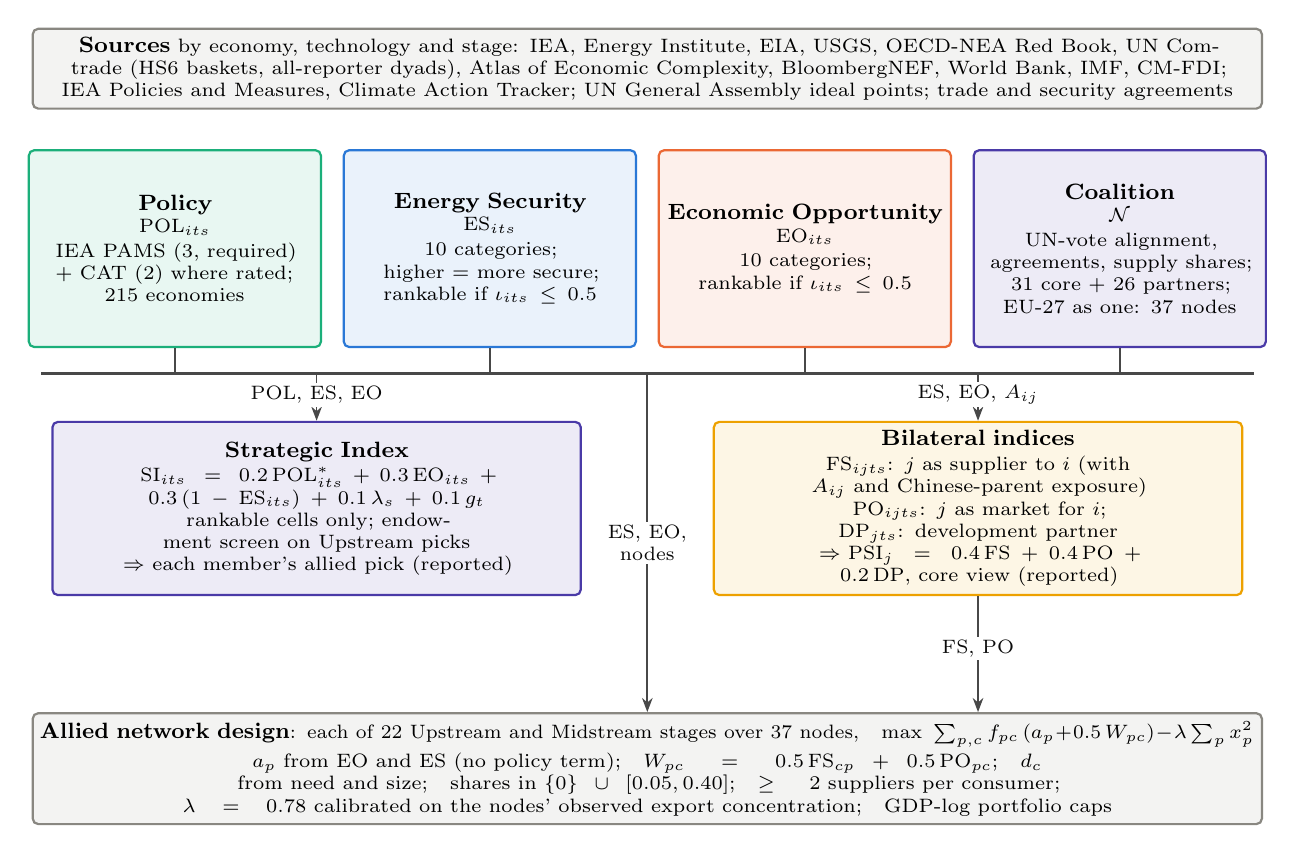
\begin{tikzpicture}[
    font=\scriptsize,
    >={Stealth[length=1.8mm]},
    box/.style={draw=#1, fill=#1!10, thick, rounded corners=2pt, align=center, inner sep=3pt,
                anchor=north},
    flow/.style={->, draw=osiink!75, line width=0.6pt},
    bus/.style={draw=osiink!75, line width=0.9pt},
    lab/.style={font=\scriptsize, text=osiink, fill=white, inner sep=1.2pt, align=center}
  ]
  \node[box=osigray, text width=15.4cm] (src) at (8, 0) {%
    {\footnotesize\bfseries Sources} by economy, technology and stage: IEA, Energy Institute,
    EIA, USGS, OECD-NEA Red Book, UN Comtrade (HS6 baskets, all-reporter dyads), Atlas of
    Economic Complexity, BloombergNEF, World Bank, IMF, CM-FDI;\\ IEA Policies and Measures,
    Climate Action Tracker; UN General Assembly ideal points; trade and security agreements};
  \node[box=osiaqua, text width=3.5cm, minimum height=2.5cm] (pol)
    at ($(src.south)+(-6,-0.5)$) {%
    {\footnotesize\bfseries Policy}\\ $\POL_{its}$\\[1pt] IEA PAMS (3, required)\\
    $+$ CAT (2) where rated;\\ 215 economies};
  \node[box=osiblue, text width=3.5cm, minimum height=2.5cm] (es)
    at ($(src.south)+(-2,-0.5)$) {%
    {\footnotesize\bfseries Energy Security}\\ $\ES_{its}$\\[1pt] 10 categories;\\
    higher $=$ more secure;\\ rankable if $\iota_{its}\le0.5$};
  \node[box=osiorange, text width=3.5cm, minimum height=2.5cm] (eo)
    at ($(src.south)+(2,-0.5)$) {%
    {\footnotesize\bfseries Economic Opportunity}\\ $\EO_{its}$\\[1pt] 10 categories;\\
    rankable if $\iota_{its}\le0.5$};
  \node[box=osiviolet, text width=3.5cm, minimum height=2.5cm] (coal)
    at ($(src.south)+(6,-0.5)$) {%
    {\footnotesize\bfseries Coalition}\\ $\Coalition$\\[1pt] UN-vote alignment,\\
    agreements, supply shares;\\ 31 core $+$ 26 partners;\\ EU-27 as one: 37 nodes};
  \coordinate (busy) at ($(src.south)+(0,-3.35)$);
  \draw[bus] ($(busy)+(-7.7,0)$) -- ($(busy)+(7.7,0)$);
  \foreach \n in {pol, es, eo, coal} {\draw[bus] (\n.south) -- (\n.south |- busy);}
  \node[box=osiviolet, text width=6.5cm, minimum height=2.2cm] (si)
    at ($(busy)+(-4.2,-0.6)$) {%
    {\footnotesize\bfseries Strategic Index}\\[1pt]
    $\SI_{its}=0.2\,\POL^{*}_{its}+0.3\,\EO_{its}+0.3\,(1-\ES_{its})+0.1\,\lambda_s+0.1\,g_t$\\
    rankable cells only; endowment screen on Upstream picks\\
    $\Rightarrow$ each member's allied pick (reported)};
  \node[box=osiyellow, text width=6.5cm, minimum height=2.2cm] (bil)
    at ($(busy)+(4.2,-0.6)$) {%
    {\footnotesize\bfseries Bilateral indices}\\[1pt]
    $\FS_{ijts}$: $j$ as supplier to $i$ (with $A_{ij}$ and Chinese-parent exposure)\\
    $\PO_{ijts}$: $j$ as market for $i$;\quad $\DP_{jts}$: development partner\\
    $\Rightarrow$ $\PSI_j=0.4\,\FS+0.4\,\PO+0.2\,\DP$, core view (reported)};
  \draw[flow] (si.north |- busy) -- node[lab, pos=0.45] {$\POL$, $\ES$, $\EO$} (si.north);
  \draw[flow] (bil.north |- busy) -- node[lab, pos=0.45] {$\ES$, $\EO$, $A_{ij}$} (bil.north);
  \node[box=osigray, text width=15.4cm] (net) at ($(busy)+(0,-4.3)$) {%
    {\footnotesize\bfseries Allied network design}: each of 22 Upstream and Midstream stages over
    37 nodes,\quad $\max\ \sum_{p,c}f_{pc}\,(a_p+0.5\,W_{pc})-\lambda\sum_p x_p^2$\\[1pt]
    $a_p$ from $\EO$ and $\ES$ (no policy term);\quad $W_{pc}=0.5\,\FS_{cp}+0.5\,\PO_{pc}$;\quad
    $d_c$ from need and size;\quad shares in $\{0\}\cup[0.05,0.40]$;\quad $\ge2$ suppliers per
    consumer;\\ $\lambda=0.78$ calibrated on the nodes' observed export concentration;\quad
    GDP-log portfolio caps};
  \draw[flow] (busy) -- node[lab, pos=0.5] {$\ES$, $\EO$,\\ nodes} (net.north);
  \draw[flow] (bil.south) -- node[lab, pos=0.45] {$\FS$, $\PO$} (bil.south |- net.north);
  \end{tikzpicture}%
  }
  \caption{Architecture of the analysis. Sources feed four cell- or economy-level constructs:
  the Policy index, the two pillars, and the coalition, derived from alignment in the UN General
  Assembly, agreements and supply shares. The Strategic Index ranks each country's sectors and
  yields the allied picks; the bilateral indices rate partners as suppliers and markets and are
  summarised in the Partnership Strength Index. The network design allocates production among
  the coalition's nodes. In the terms of \citet{neis2026allied}, the pillars, the Policy index and
  the Strategic Index address relative exposure and capability, the coalition and the bilateral indices
  complementarity, and the network design specialisation and, in part, robustness. $\iota_{its}$
  is the imputed share of a cell's index weight; the Strategic Index and the Partnership Strength
  Index are not inputs to the network design.}
  \label{fig:framework_architecture}
\end{figure}

\begin{table}[tbp]
\centering
\begin{threeparttable}
\caption{How security and opportunity enter each index}
\label{tab:roles}
\footnotesize
\begin{tabularx}{\textwidth}{@{}>{\raggedright\arraybackslash}p{2.7cm}
  >{\raggedright\arraybackslash}p{2.4cm} >{\raggedright\arraybackslash}X
  >{\raggedright\arraybackslash}X@{}}
\toprule
Index & Whose position & Energy security enters as & Economic opportunity enters as\\
\midrule
Strategic Index $\SI_{its}$ & country $i$, deciding where to build &
  need of $i$: $1-\ES_{its}$ (level), weight 0.3 &
  capability of $i$: $\EO_{its}$ (level), weight 0.3\\[2pt]
Friendshore $\FS_{ijts}$ & importer $i$, supplier $j$ &
  need of the importer, ranked across $i$'s own cells, weight 2 of 11 &
  capability of the supplier, ranked across economies in $(t,s)$, weight 2 of 11\\[2pt]
Partnership Opportunity $\PO_{ijts}$ & exporter $i$, market $j$ &
  need of the market, ranked across markets, weight 1 of 7 &
  capability of the exporter, ranked across economies, weight 3 of 7\\[2pt]
Development Potential $\DP_{jts}$ & partner $j$, not high income &
  need of the partner, weight 1 of 10 & opportunity of the partner, weight 1.5 of 10\\[2pt]
Network producer score $a_p$ & node $p$ as producer &
  security of the producer, S-curve across nodes, weight 2/7 &
  capability of the producer, S-curve across nodes, weight 5/7\\[2pt]
Network demand $d_c$ & node $c$ as consumer &
  need of the consumer, weight 0.5 (with size, 0.5) & ---\\
\bottomrule
\end{tabularx}
\begin{tablenotes}[flushleft]\footnotesize
\item \textit{Notes:} Weights are nominal, before renormalisation over the components observed.
Security enters as need wherever it describes the party that would gain from new supply, and as
security only in the producer score of the network design, where a node's own security in a
stage proxies its reliability as a supplier. Sections~\ref{sec:strategic}, \ref{sec:bilateral}
and~\ref{sec:network} give the full definitions.
\end{tablenotes}
\end{threeparttable}
\end{table}

\begin{table}[tbp]
\centering
\begin{threeparttable}
\caption{Notation}
\label{tab:notation}
\footnotesize
\begin{tabularx}{\textwidth}{@{}>{\raggedright\arraybackslash}p{2.9cm}
  >{\raggedright\arraybackslash}X >{\raggedright\arraybackslash}p{2.7cm}@{}}
\toprule
Symbol & Meaning & Defined in\\
\midrule
\multicolumn{3}{@{}l}{\textit{Sets and indices}}\\
$\Countries$ & the 219 economies after harmonisation & Sec.~\ref{sec:data}\\
$\Techs$, $\Stages$ & eleven headline technologies; \{Upstream, Midstream, Downstream\} &
  Sec.~\ref{subsec:framework_unit}\\
$\Coalition$ & the 57 coalition members (31 core, 26 partners); 37 network nodes &
  Sec.~\ref{sec:coalition}\\
$i,j$; $t,s$; $k,v$ & economy (reporter), partner; technology, stage; category, variable & \\
$p,c$ & network node as producer; as consumer & Sec.~\ref{sec:network}\\
$\cell$, $\dyad$ & cell; directed dyad with reporter $i$ and partner $j\neq i$ &
  Secs.~\ref{subsec:framework_unit}, \ref{sec:bilateral}\\[2pt]
\multicolumn{3}{@{}l}{\textit{Normalisation and pillars}}\\
$x_{itsv}$, $r$ & raw variable; percent rank within comparison set $g$ & Eq.~\eqref{eq:fw_scurve}\\
$\Scurve$, $\gamma$ & S-curve; curvature, $\gamma=0.5$; ${\Scurve}[\cdot]_g$ ranks within $g$ &
  Eq.~\eqref{eq:fw_scurve}\\
$\tilde x_{itsv}$, $\hat x_{itsv}$ & theme index; after the missing-data rule &
  Eqs.~\eqref{eq:fw_scurve}, \eqref{eq:fw_category}\\
$c_{itsk}$, $w^{P}_k$ & category score; weight of category $k$ in pillar $P$ &
  Eqs.~\eqref{eq:fw_category}, \eqref{eq:fw_pillar}\\
$\ES_{its}$, $\EO_{its}$ & Energy Security and Economic Opportunity pillars, in $[0,1]$ &
  Eq.~\eqref{eq:fw_pillar}\\
$\iota_{its}$ & imputed share of the cell's index weight; rankable if $\iota_{its}\le0.5$ &
  Eq.~\eqref{eq:rankable}\\[2pt]
\multicolumn{3}{@{}l}{\textit{Policy and Strategic Index}}\\
$\POL_{its}$, $\POL^{*}_{its}$ & Policy index; its S-curve across $i$'s scored sectors &
  Eqs.~\eqref{eq:pol_composite}, \eqref{eq:si_pol}\\
$\lambda_s$, $g_t$ & stage weight; technology emissions weight (1 = cleanest) &
  Eqs.~\eqref{eq:fw_si}, \eqref{eq:ghg_index}\\
$\SI_{its}$ & Strategic Index & Eq.~\eqref{eq:fw_si}\\[2pt]
\multicolumn{3}{@{}l}{\textit{Alignment and bilateral indices}}\\
$s_i$, $A_{ij}$ & position on the U.S.--China axis; dyadic alignment &
  Eqs.~\eqref{eq:coalition_axis}, \eqref{eq:coalition_dyadic}\\
$\FS_{ijts}$, $\PO_{ijts}$, $\DP_{jts}$ & Friendshore; Partnership Opportunity; Development
  Potential & Eqs.~\eqref{eq:fs_index}, \eqref{eq:po_index}, \eqref{eq:dp_index}\\
$\PSI_j$ & Partnership Strength Index & Eq.~\eqref{eq:psi}\\[2pt]
\multicolumn{3}{@{}l}{\textit{Network design}}\\
$a_p$, $W_{pc}$, $d_c$ & producer score; edge weight; demand weight ($\sum_c d_c=1$) &
  Eq.~\eqref{eq:fw_network}\\
$y_p$, $\ell_{pc}$, $f_{pc}$, $x_p$ & producer selection; supplier link; flow share; production
  share & Eq.~\eqref{eq:fw_network}\\
$\lambda$, $\HHI$ & diversification weight; Herfindahl--Hirschman index & Eq.~\eqref{eq:fw_network}\\
\bottomrule
\end{tabularx}
\begin{tablenotes}[flushleft]\footnotesize
\item \textit{Notes:} The stage weight $\lambda_s$ carries a subscript and the diversification
weight $\lambda$ none; the axis position $s_i$ carries an economy subscript and the stage $s$
none. The production share $x_p$ and the policy components $x^{v}_{its}$ of
Section~\ref{sec:strategic} are distinct from the raw variable $x_{itsv}$. Later sections
introduce further symbols where they are needed.
\end{tablenotes}
\end{threeparttable}
\end{table}

% =============================================================================
% Section 3: Data
% Specification: config/raw_inputs_manifest.yml, docs/sources.md, docs/methodology.md,
%   scripts/10_build_themes.R, scripts/12-15, scripts/98_pull_comtrade_energy_dyads.R,
%   R/utils/country.R, R/categories/trade/trade_core.R, data/reference/energy_hs6_master.csv.
% Numbers: paper/results/method.json, hs6_crosswalk.json, bilateral.json, coalition.json
%   (final rerun of 12 October 2026). Release rule, harmonisation, vintages and the years of
%   each source: Online Appendix oa:data (sections/oa_data.tex).
% =============================================================================

\section{Data}\label{sec:data}

The indices combine public statistical releases, licensed commercial datasets and a few
project-authored tables. Appendix~\ref{app:sources} lists every source with its publisher,
coverage and release, Appendix~\ref{app:variables} every variable built from it, and Online
Appendix~\ref{oa:data} the rule that selects a release, the harmonisation of economy names and
the years each source covers.

% -----------------------------------------------------------------------------
\subsection{Sources by pillar}\label{subsec:data_families}

Table~\ref{tab:data_families} groups the sources by what they measure. Most report economies,
but some report the world (commodity prices, demand projections, technology readiness) or a few
regions (manufacturing capacity, relative equipment costs); such a variable shifts a pair's level
without ranking economies within it. Coverage ranges from about two hundred economies for trade
and energy statistics to a few dozen for levelised costs, a gap that the missing-data rules of
Section~\ref{subsec:norm_missing} bridge.

\begin{table}[tbp]
\centering
\begin{threeparttable}
\caption{Source families, levels of observation and what they feed}
\label{tab:data_families}
\footnotesize
\begin{tabularx}{\textwidth}{@{}>{\raggedright\arraybackslash}p{2.3cm}
  >{\raggedright\arraybackslash}X >{\raggedright\arraybackslash}p{2.0cm}
  >{\raggedright\arraybackslash}p{4.2cm}@{}}
\toprule
Family & Sources & Level & Feeds\\
\midrule
Energy statistics & EI Statistical Review 2026; EIA International Energy Statistics (fuel
  production EI does not report) & Economy & ES: energy access, consumption, energy imports,
  reserves (fossil), production (minerals). EO: energy access, production\\[2pt]
Reserves and uranium & USGS Mineral Commodity Summaries 2026; OECD-NEA/IAEA Red Book (Uranium
  2026); EI proved reserves & Economy & ES: reserves, production (uranium). EO: production
  (uranium). Coalition supplier test\\[2pt]
Trade & UN Comtrade all-reporter dyads (2020, 2024) and their World totals; Atlas of Economic
  Complexity (HS92); Comtrade critical-minerals extracts & Economy; dyad & ES: trade, minerals
  trade. EO: trade. Friendshore, Partnership Opportunity, network edges\\[2pt]
Minerals and manufacturing & IEA Critical Minerals Dataset 2026; IEA ETP 2024 capacity shares;
  IEA EV regional data & Economy; 5--6 regions & ES and EO: foreign dependency, production;
  mineral demand weights\\[2pt]
Demand and technology & IEA WEO 2025; IEA Global EV Outlook 2026; BNEF New Energy Outlook 2024
  and Supply Chains 2025; BCG market sizing; IEA Clean Energy Technology Guide & World; region;
  United States & ES: consumption. EO: consumption, technology demand, technological
  readiness\\[2pt]
Costs and prices & BNEF LCOE; IEA relative costs; ILOSTAT earnings; IMF lending rates, producer
  prices and commodity prices & Economy; region; world & ES: energy prices. EO: cost
  competitiveness, energy prices\\[2pt]
Potential and investment & Global Solar and Wind Atlases; geothermal potentials; Clean
  Investment Monitor & Economy & ES: reserves (downstream). ES and EO: investment\\[2pt]
Policy & IEA Policies and Measures; Climate Action Tracker; IPCC lifecycle emissions; GTA NIPO
  (robustness only) & Economy; technology & Policy index; technology weight of the SI\\[2pt]
Bilateral and alignment & IMF Direct Investment Positions; CM-FDI projects; WDI; Doing Business;
  OECD CRS; UNGA ideal points; agreement memberships & Dyad; economy & PSI components; blocs,
  coalition, network demand and caps\\
\bottomrule
\end{tabularx}
\begin{tablenotes}[flushleft]\footnotesize
\item \textit{Notes:} ES = Energy Security; EO = Economic Opportunity; SI = Strategic Index;
PSI = Partnership Strength Index. A source reported for a region or for the world is copied to
the economies it covers by the theme that reads it. Appendix~\ref{app:sources} gives publishers,
coverage and releases; Appendix~\ref{app:variables} the variables.
\end{tablenotes}
\end{threeparttable}
\end{table}

\paragraph{Energy security.} The Statistical Review of World Energy \citep{ei2026statistical},
2026 edition with data to 2025, supplies consumption per capita and its growth, the fuel balances
behind energy imports, mineral production and the proved reserves of oil, gas and coal, which the
Review holds at end-2020. Fossil production that the Review counts only in a regional residual
is taken from the U.S. Energy Information Administration \citep{eia2026international}, in the
Review's units and paired with consumption of the same year, as an observation (Estonian coal,
where the Review counts oil shale, stays missing). Critical-mineral reserves at end-2025 (cobalt,
lithium, graphite, rare earths, copper, manganese, nickel, zinc and the platinum-group metals)
come from the USGS Mineral Commodity Summaries 2026 \citep{usgs2026mcs}, with the erratum that
puts Brazil's rare-earth reserves at 11~Mt; holders listed without a figure (``NA'', ``W'',
``s'') count as zero in the technology roll-ups. Nuclear Upstream is scored on the OECD-NEA/IAEA
Red Book \citep{oecdnea2026uranium}: identified recoverable resources below USD 260/kgU at
1 January 2025 (59 economies) and mine production in 2019--2024 (18 producers in 2024), with
economies absent from the tables recorded as zero. The IEA Critical Minerals Dataset
\citep{iea2026cmdata} provides mining (Upstream) and refining (Midstream) supply by economy and
the clean-technology demand that weights each mineral within a technology. Midstream capacity
shares come from IEA Energy Technology Perspectives \citep{iea2024etp}, taken over the world total
including the source's ``Other'' row. Its 2035 announced-capacity shares are regional for
Europe, so every EU member carries the EU's share (0.15 in Wind, 0.11 in Batteries, 0.24 in Green
Hydrogen and 0.00 in Solar Midstream) in the foreign-dependency and market-share variables, which
therefore do not separate the members. Commodity prices (IMF Primary Commodity Price System, \citealp{imf2026pcps}),
clean-technology investment (Clean Investment Monitor, \citealp{cim2026}) and three geospatial
resource-potential datasets complete the pillar.

\paragraph{Economic opportunity.} Export capability rests on the Growth Lab's reconciled HS92 data
underlying the Atlas of Economic Complexity \citep{growthlab2019trade,hausmann2014atlas}, newest
year 2023, and on the 2024 Comtrade exports of Section~\ref{subsec:data_trade}. Demand comes from
the IEA World Energy Outlook 2025 and Global EV Outlook 2026 \citep{iea2025weo,iea2026gevo},
BloombergNEF's New Energy Outlook 2024 \citep{bnef2024neo} and Supply Chains 2025 workbook, and a
Boston Consulting Group sizing of the U.S. addressable market. Costs combine BloombergNEF levelised
costs, IEA relative equipment costs, ILOSTAT earnings, IMF lending rates (placeholder zero
readings dropped) and producer prices. The BloombergNEF and BCG inputs are licensed, which
prevents a fully public replication of this pillar.

\paragraph{Technology readiness by stage.} The IEA Clean Energy Technology Guide
\citep{iea2026cleantechguide} rates technology designs and components on an eleven-point
readiness scale. Ordered rules assign each item to a technology and a stage or classify it as out
of scope: 253 of the 634 items of the 2026 release map to a headline technology. A cell's
readiness is computed from the items of its own stage; a stage without an item, 10 of the 33
cells, takes the technology-wide value. Readiness has no country dimension and is copied to every
economy as an observation.

\paragraph{Policy.} The Policy index combines the IEA Policies and Measures database
\citep{iea2026pams} (export of 22 January 2026), weight 3, and the Climate Action Tracker ratings
\citep{cat2026ratings} (39 countries and the EU, whose rating its unrated members take), weight 2.
IEA PAMS is required and CAT added where it rates the country: 215 economies are scored, 65 on
both and 150 on IEA PAMS alone (Section~\ref{sec:strategic}). The New Industrial Policy
Observatory of Global Trade Alert \citep{gta2026nipo} enters only a robustness variant
(Section~\ref{sec:robustness}). The technology weight of the Strategic Index uses the IPCC
lifecycle-emission medians \citep{schlomer2014annex}.

\paragraph{Bilateral, alignment and coalition inputs.} Outward direct-investment positions come
from the IMF Direct Investment Positions dataset. Positions with 16 conduit financial centres,
the ten pass-through economies identified by \citet{damgaard2024real} and six offshore centres
(Appendix~\ref{app:variables}), are treated as unobserved on either side of the dyad. In battery, electric-vehicle, solar and wind manufacturing, the investment tie and the
Chinese-parent exposure of Friendshore come instead from the Cleantech Manufacturing FDI dataset
\citep{bandara2026cmfdi}, of whose 1,042 cross-border projects 905 qualify. Development potential
uses the World Development Indicators \citep{worldbank2026wdi}, the 2019 Doing Business scores
\citep{worldbank2020doing,worldbank2021discontinue} and OECD aid data. Geopolitical alignment
uses the all-votes UN General Assembly ideal points of \citet{bailey2017estimating} (Dataverse
V39, \citealp{voeten2009unga}), averaged over sessions 74--78 (2019--2023), and coalition
membership a project-authored list of U.S. free-trade agreements, IPEF, the Minerals Security
Partnership, the G7 and NATO compiled from the official lists (Section~\ref{sec:coalition}).

% -----------------------------------------------------------------------------
\subsection{The HS6 product crosswalk}\label{subsec:data_crosswalk}

Trade enters through baskets of six-digit Harmonized System (HS6) products, one per
technology--stage pair, defined in one version-controlled table
(\texttt{data/reference/energy\_hs6\_master.csv}) from which every trade and bilateral file is
generated. With $H_{ts}$ the codes in the basket of $(t,s)$ and $x_{ih}$ economy $i$'s exports of
product $h$, basket exports are
\begin{equation}\label{eq:data_basket}
  X_{its}=\sum_{h\in H_{ts}}x_{ih},
\end{equation}
and imports, world totals and bilateral flows are aggregated in the same way. Ores,
concentrates, slag and scrap are Upstream, processed materials and components Midstream;
Downstream activity is not a traded-goods stage.

\paragraph{The basket review.} In October 2026 every code was tested for dominant use: it stays
in a technology's basket only if that technology is a main use of the product. Ninety-two basket
rows touching 69 codes failed (47 codes left every basket); each stays in the master with its
reason. The crosswalk now holds 259 codes in 415 basket rows (298 in 490 before): 242 of the
current nomenclature and 17 legacy codes that bridge the HS92 Atlas panels. The exclusions carried
92 percent of the pre-review coal Midstream basket's trade, 69 percent of gas Midstream and 89
percent of batteries Upstream, whose copper ores now belong to the grid
(Table~\ref{tab:hs6_counts}). Electric Grid Upstream held only electrical energy (HS 2716.00),
which made net power exporters the grid's leading suppliers; it now holds seven copper and
aluminium inputs, from ores and bauxite to cathodes and unwrought aluminium, so electricity is
outside every basket. Switching and routing apparatus (HS 8517.62), 32 percent of the pre-review
grid Midstream basket, is telecommunication equipment and left it.

\paragraph{Upstream baskets.} Five Upstream baskets are new: Electric Vehicles (the battery-mineral
ores and the rare earths of permanent magnets), Wind (rare earths), Nuclear (uranium ores and
natural uranium compounds, the heading of most yellowcake, moved from Midstream), Solar (silicon
metal) and Semiconductors (gallium, germanium and indium, carried for description only). The four
that are scored trade USD 3.0 billion (wind) to 21.3 billion (electric vehicles) in 2024. With
them, 18 of the 22 scored Upstream and Midstream pairs have a basket; only Geothermal and Green
Hydrogen have none.

\paragraph{A many-to-many mapping.} The baskets do not partition the product space: 105 codes
(41 percent) belong to more than one basket, 63 to two, 33 to three and 9, the transformer,
switchgear and cable headings, to four, since a power cable is an input to every technology that
connects to the grid. Technology totals are therefore not additive, and the trade variables of
technologies that share codes are mechanically correlated.

\begin{figure}[tbp]
  \centering
  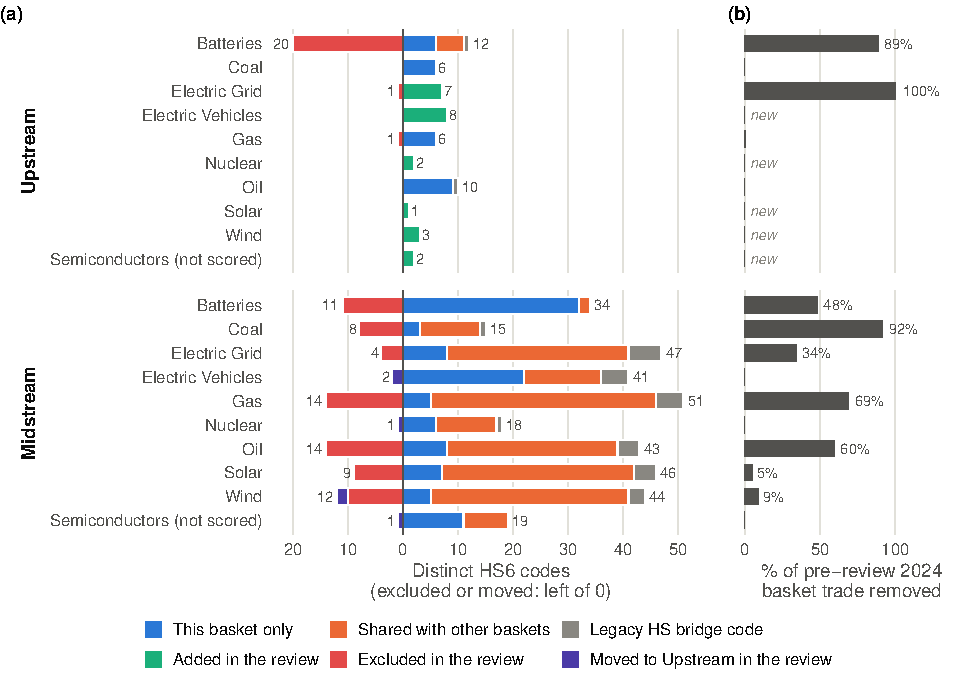
\includegraphics[width=\textwidth]{fig_hs6_crosswalk}
  \caption{The HS6 baskets after the October 2026 review. Panel (a): distinct HS6 codes in each
  technology--stage basket, split into codes of that basket only, current codes shared with at
  least one other basket (the many-to-many part of the mapping), legacy HS bridge codes, and codes
  added by the review (codes moved from a technology's midstream basket count as added to its
  upstream basket); left of zero, the codes the review excluded from the basket and the codes it
  moved to the upstream stage. Panel (b): share of the pre-review basket's 2024 trade value carried
  by the excluded codes; ``new'' marks a basket the review created. Trade is the reconciled
  all-reporter Comtrade matrix (the importer's declaration, else the exporter's declaration
  $\times1.06$), summed over exporter--importer pairs; a code in several baskets counts in each.
  Green hydrogen, geothermal and the downstream stage have no basket; semiconductors are carried
  in the master but not scored. Source: \texttt{data/reference/energy\_hs6\_master.csv},
  \texttt{data/raw/comtrade\_energy\_dyads\_all.csv}; \texttt{scripts/paper/fig\_hs6\_crosswalk.R}.}
  \label{fig:hs6_crosswalk}
\end{figure}

% Generated by scripts/paper/fig_hs6_crosswalk.R; do not edit by hand.
\begin{table}[tbp]
\centering
\begin{threeparttable}
\caption{HS6 baskets by technology and stage after the October 2026 basket review}
\label{tab:hs6_counts}
\footnotesize
\setlength{\tabcolsep}{3.5pt}
\begin{tabular}{@{}llrrrrrrrrr@{}}
\toprule
 & & \multicolumn{4}{c}{Codes in the basket} & \multicolumn{3}{c}{Review} & \multicolumn{2}{c}{Basket trade, 2024} \\
\cmidrule(lr){3-6}\cmidrule(lr){7-9}\cmidrule(l){10-11}
Technology & Stage & All & Legacy & Shared & Sub-sectors & Added & Moved & Excluded & USD bn & \% removed\\
\midrule
Batteries & Upstream & 12 & 1 & 5 & 2 & 0 & 0 & 20 & 21.2 & 88.8\\
 & Midstream & 34 & 0 & 2 & 9 & 0 & 0 & 11 & 202.7 & 48.4\\
Coal & Upstream & 6 & 0 & 0 & 2 & 0 & 0 & 0 & 192.5 & 0.0\\
 & Midstream & 15 & 1 & 12 & 3 & 0 & 0 & 8 & 20.5 & 91.9\\
Electric Grid & Upstream & 7 & 0 & 0 & 3 & 7 & 0 & 1 & 321.0 & 100.0\\
 & Midstream & 47 & 6 & 36 & 12 & 0 & 0 & 4 & 449.6 & 34.3\\
Electric Vehicles & Upstream & 8 & 0 & 8 & 8 & 8 & 0 & 0 & 21.3 & new\\
 & Midstream & 41 & 5 & 17 & 7 & 0 & 2 & 0 & 1,003.2 & 0.0\\
Gas & Upstream & 6 & 0 & 0 & 4 & 0 & 0 & 1 & 445.3 & 0.4\\
 & Midstream & 51 & 5 & 46 & 2 & 0 & 0 & 14 & 151.6 & 69.1\\
Nuclear & Upstream & 2 & 0 & 0 & 2 & 2 & 0 & 0 & 11.4 & new\\
 & Midstream & 18 & 1 & 12 & 3 & 0 & 1 & 0 & 24.6 & 0.0\\
Oil & Upstream & 10 & 1 & 0 & 5 & 0 & 0 & 0 & 2,211.0 & 0.0\\
 & Midstream & 43 & 4 & 35 & 7 & 0 & 0 & 14 & 127.1 & 59.8\\
Solar & Upstream & 1 & 0 & 0 & 1 & 1 & 0 & 0 & 3.8 & new\\
 & Midstream & 46 & 4 & 38 & 9 & 0 & 0 & 9 & 711.5 & 5.5\\
Wind & Upstream & 3 & 0 & 3 & 3 & 3 & 0 & 0 & 3.0 & new\\
 & Midstream & 44 & 3 & 39 & 8 & 0 & 2 & 10 & 409.5 & 9.4\\
Semiconductors\tnote{a} & Upstream & 2 & 1 & 0 & 1 & 2 & 0 & 0 & 1.1 & new\\
 & Midstream & 19 & 0 & 8 & 8 & 0 & 1 & 0 & 1,348.1 & 0.0\\
\midrule
Distinct codes & & 259 & 17 & 105 & 92 & 20 & 4 & 69 & & \\
\bottomrule
\end{tabular}
\begin{tablenotes}[flushleft]\footnotesize
\item \textit{Notes:} Distinct HS6 codes in each technology--stage basket of \texttt{data/reference/energy\_hs6\_master.csv} after the review. ``Legacy'' codes are bridge codes of older HS revisions whose successors are all in the basket; ``Shared'' counts the codes that also belong to at least one other basket. ``Excluded'' counts the codes the review removed from the basket because the technology is not a dominant use of the product, and ``Added'' the codes it added (the copper and aluminium inputs that replace electrical energy, HS 2716.00, in electric-grid Upstream, and the Upstream baskets of electric vehicles, solar, wind, nuclear and semiconductors, which had none); ``Moved'' counts the codes it moved from a technology's Midstream to its Upstream basket (rare-earth compounds and metals, natural uranium compounds, unwrought gallium, germanium and indium), which count as added there, since a code sits in one stage of a technology; the rows stay in the master with the reason. Basket trade is the 2024 value in the reconciled all-reporter Comtrade matrix (the importer's declaration, else the exporter's mirror declaration $\times$ 1.06), summed over exporter--importer pairs; ``\% removed'' is the share of the pre-review basket's value carried by the excluded codes (moved codes are not removals; ``new'' marks a basket the review created). A code in several baskets counts in each, so neither codes nor trade values add across rows. Green hydrogen, geothermal and the Downstream stage have no basket.
\item[a] Carried in the master; not a scored technology.
\end{tablenotes}
\end{threeparttable}
\end{table}


% -----------------------------------------------------------------------------
\subsection{Bilateral trade and the trade themes}\label{subsec:data_trade}

Bilateral flows come from an all-reporter pull of UN Comtrade \citep{uncomtrade} for the
endpoint years 2020 and 2024: 173 economies report in at least one year (168 in 2020; 142 for
exports and 143 for imports in 2024), and 208 appear as reporter or partner. Comtrade records
Taiwan as ``Other Asia, n.e.s.'' (partner code S19), which is mapped to Taiwan's own code. Let
$M^{\mathrm{rep}}_{ji,h}$ be importer $j$'s declared imports of product $h$ from $i$ and
$X^{\mathrm{rep}}_{ij,h}$ exporter $i$'s declared exports to $j$. The flow in a cell is
\begin{equation}\label{eq:data_mirror}
  F_{ij,ts}=
  \begin{cases}
    \sum_{h\in H_{ts}}M^{\mathrm{rep}}_{ji,h} & \text{if $j$ reports imports in the cell that year},\\
    1.06\sum_{h\in H_{ts}}X^{\mathrm{rep}}_{ij,h} & \text{otherwise, if $i$ reports exports to $j$},
  \end{cases}
\end{equation}
and unobserved otherwise; 1.06 is the IMF's conventional ratio of CIF import to FOB export values.
Of the 701,214 exporter--importer--technology--stage cells observed in 2024, 22 percent are
mirror values, but only 13 percent of the cells with positive trade and 4 percent of the value,
because large traders report. Thirty importers that reported in 2020 did not in 2024, among them
Russia, Iran, the United Arab Emirates and Viet Nam, and 65 of the 208 importers enter the 2024
matrix only through their partners' declarations, which omits their imports from exporters that
do not report either.

The country-level trade themes read a file of exports and imports by reporter and code rebuilt
from the World rows of the same pull: 142 exporting and 143 importing reporters in 2024 and every
current-nomenclature basket code, including Qatar's exports of liquefied natural gas (USD 56.9
billion), which the earlier extract omitted. Hong Kong is left out of the Comtrade export measures
(export size, revealed comparative advantage \citep{balassa1965trade} and export concentration)
because its exports are mostly re-exports that the producers' own exports already count; it keeps
its Atlas-based variables, and the bilateral matrix is not filtered. The export-concentration
index is ranked across the cells of the eleven headline technologies only. Critical-minerals
trade uses separate 2024 Comtrade extracts (130 import and 128 export reporters); the 2025
extracts, with three reporters, fall below the coverage floor of the release rule (Online
Appendix~\ref{oa:data}).

% -----------------------------------------------------------------------------
\subsection{Economies, coverage and rankability}\label{subsec:data_countries}

Every economy name in every source is mapped to one canonical name per ISO3 code before anything
is ranked, and world, regional, residual and historical aggregates are dropped. The headline
pillars then cover 219 economies, each with its own ISO3 code, of which 195 are sovereign states
(the 193 members of the United Nations, Kosovo and Taiwan) and 24 are territories, special
administrative regions or the West Bank and Gaza; the same 219 economies (195 sovereign states and
24 territories) have an $\EO$ score, so the two pillars share one universe. Taiwan, which the
World Bank's country table does not list, is carried as an economy throughout, including the trade
themes and the bilateral matrix; it has an $\ES$ value in 28 headline cells and an $\EO$ value in
33. The pillars score 6,232 $\ES$ and 7,131 $\EO$ country--technology--stage cells in 30 and 33
headline pairs. In the alignment data the 193 economies that vote in the General Assembly have an
ideal point; the other economies are treated as Section~\ref{sec:coalition} describes.

The grids span almost the whole universe at every stage, but their width is set by the most
widely distributed theme of each pair. Figure~\ref{fig:method_coverage} separates economies scored
from economies with country-specific data. In $\ES$ the two differ only upstream, where a
commodity-price series copied to every economy sets the grid: by 4 economies in Electric Vehicles
to 38 in Coal, and not at all in Nuclear once absence from the uranium registers is recorded as
zero. In $\EO$ the gap is largest in Electric Grid downstream (143 of 213 economies with
country-specific data). Territories rest more heavily on imputation (mean imputed weight 0.48 of a
territory's $\ES$ cell against 0.29 for a sovereign state; 0.67 against 0.40 in $\EO$).

\begin{figure}[tbp]
  \centering
  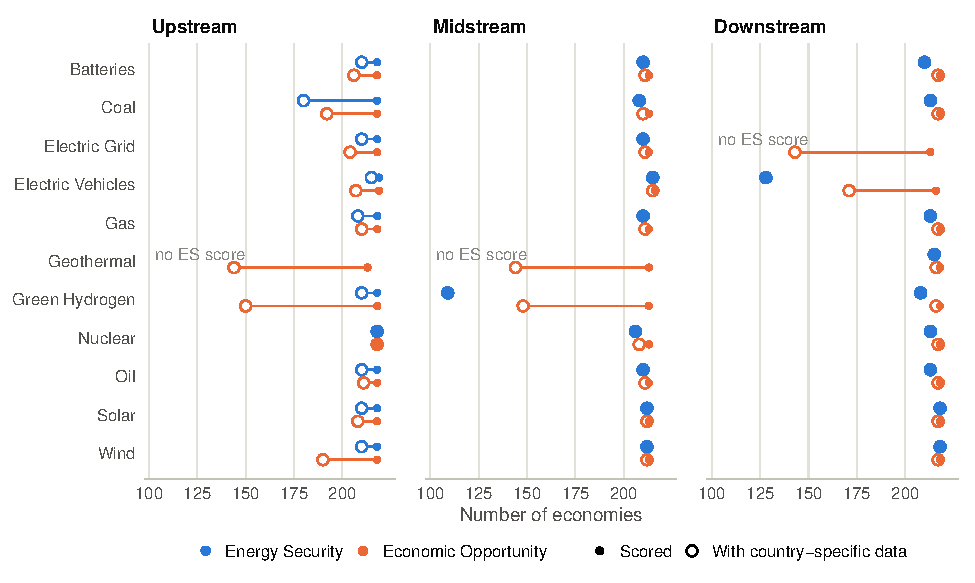
\includegraphics[width=\textwidth]{method_coverage}
  \caption{Economies scored and economies with country-specific data, by technology--stage pair.
  Filled dots: the number of economies with a pillar value in the pair. Hollow circles: the
  number of those economies for which at least one positively weighted, non-imputed component is
  country-specific, that is, takes at least two distinct observed values across the economies of
  the pair. World-level series copied to every economy, such as commodity-price volatility, world
  export concentration and technology readiness, do not count as country-specific. The segment
  between the two marks is the number of economies whose value rests only on imputed components
  and world-level series; where the two counts coincide the marks appear as a ringed dot. ``No ES
  score'' marks the pairs without an $\ES$ value. Every pair has status ok (no pair is constant
  or unscored). The axis starts at 100 economies. Sample: the eleven headline technologies.
  Source: variable contributions and pillar diagnostics in
  \texttt{data/processed/outputs/index\_outputs.rds}; \texttt{scripts/paper/fig\_method.R}.}
  \label{fig:method_coverage}
\end{figure}

Because coverage is uneven, every cell is scored but not every cell is ranked: a cell enters a
ranking, a top-$N$ list, the Strategic Index or the partner rankings only if the economy is
sovereign and at most half of its index weight rests on imputed components
(Section~\ref{subsec:norm_rankability}). The rule keeps 4,163 of the 6,232 $\ES$ cells and 4,301
of the 7,131 $\EO$ cells. Each component is taken at the latest year its source reports, so a cell
can combine observations from 2023 to 2025 with projections to 2035 and, in $\ES$ reserves,
end-2020 fossil stocks (Section~\ref{subsec:norm_latest}).

% ---------------------------------------------------------------------------
% Section 4: Index construction -- normalisation, imputation and aggregation
% Specification: R/utils/scurve.R (median_scurve), R/indices/index_builder_core.R (latest year,
%   missing-data policy, overall variables, available-case pillar, decompositions, diagnostics,
%   flag_rankable_cells), R/indices/build_energy_security_index_v2.R,
%   R/indices/build_economic_opportunity_index_v2.R, config/index_definition.yml,
%   config/missing_data.yml, config/weights.yml, config/rankability.yml.
% Numbers: paper/results/method.json and scurve.json (final rerun of 12 October 2026).
% Derivations, the construction algorithm and further diagnostics: Online Appendix
%   oa:normalization (sections/oa_normalization.tex).
% ---------------------------------------------------------------------------

\section{Index construction: normalisation, imputation and aggregation}\label{sec:normalization}

Construction has two layers. In the \emph{theme layer} each source's builder orients its raw
metrics (higher means more security or more opportunity) and maps them to the unit interval by a
rank-based S-curve. In the \emph{aggregation layer} the latest observation of each variable is
selected, gaps are filled by explicit rules, and variables are averaged into categories and
categories into pillars; nothing is re-ranked there. Online Appendix~\ref{oa:normalization} gives
the construction algorithm, the derivations and further diagnostics.

% ---------------------------------------------------------------------------
\subsection{Percent ranks and the median S-curve}\label{subsec:scurve}

Let $x=(x_a)_{a\in A}$ be the values of an oriented raw variable over a comparison set $A$ with
$n$ non-missing values. The percent rank and the normalised value, restating
equation~\eqref{eq:fw_scurve}, are
\begin{equation}\label{eq:pct_rank}
  r_a=\begin{cases}
    \dfrac{\rank(x_a)-1}{n-1}, & n\ge 2,\\[6pt]
    0, & n=1,
  \end{cases}
\end{equation}
\begin{equation}\label{eq:scurve}
  \Scurve(r_a)=\frac{r_a^{\gamma}}{r_a^{\gamma}+(1-r_a)^{\gamma}},\qquad \gamma=0.5 ,
\end{equation}
with ties given the average of the ranks they occupy; a missing value stays missing. We write
$\Scurve[x]_g$ for the transform taken separately within each cell of a grouping $g$. The
function is the one-parameter probability-weighting function of \citet{karmarkar1978subjectively}
applied to ranks rather than probabilities, the unit-elevation member of the linear-in-log-odds
family of \citet{gonzalez1999shape}:
\begin{equation}\label{eq:scurve_logit}
  \operatorname{logit}\Scurve(r)=\gamma\,\operatorname{logit}r .
\end{equation}

The curve is median-centred ($\Scurve(0)=0$, $\Scurve(1/2)=1/2$, $\Scurve(1)=1$ for every
$\gamma$), ordinal, hence insensitive to outliers \citep{conover1981rank}, and symmetric,
$\Scurve(1-r)=1-\Scurve(r)$. With $\gamma<1$ it is an inverse S: the bottom and top tenths of a
comparison set occupy $[0,0.25]$ and $[0.75,1]$, while the middle half is compressed into an
interval of width 0.27 (0.5 under the percent rank). The choice $\gamma=0.5$ is a stated value
judgement: moving into the lead of a distribution, or out of its bottom, is worth more than an
equal move in rank within the middle, so dominance and absence, the distinctions most relevant to
supply security, are set apart (Figure~\ref{fig:scurve}). Section~\ref{sec:robustness} varies
$\gamma$.

\begin{figure}[tbp]
  \centering
  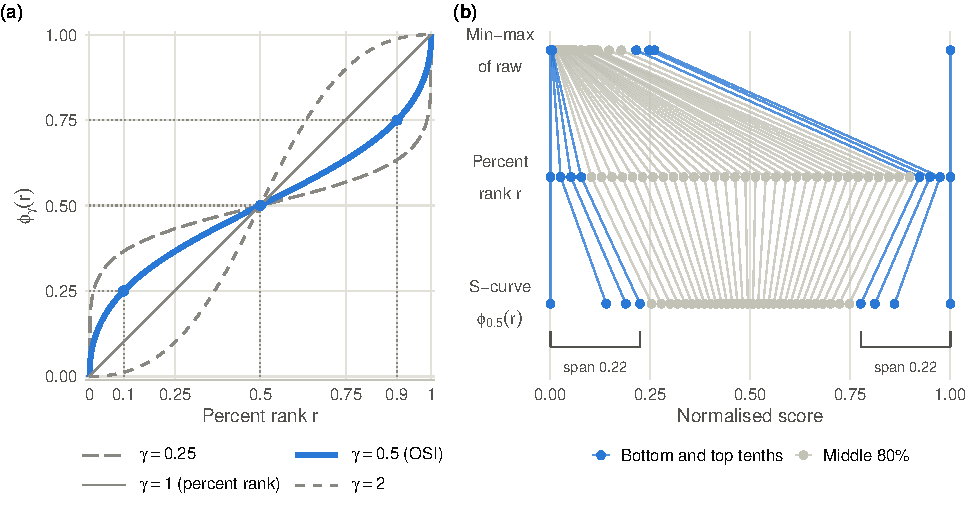
\includegraphics[width=\textwidth]{fig_scurve}
  \caption{The median-centred S-curve. Panel (a): $\Scurve(r)=r^{\gamma}/[r^{\gamma}+(1-r)^{\gamma}]$
  against the percent rank $r$ for $\gamma\in\{0.25,0.5,1,2\}$. The highlighted curve is
  $\gamma=0.5$, the value used for every component of the indices, and the marked points are
  $\Scurve(0.1)=0.25$, $\Scurve(0.5)=0.5$ and $\Scurve(0.9)=0.75$; $\gamma=1$ is the percent rank
  itself. Panel (b): 40 draws of a right-skewed variable (lognormal, log-mean 0, log-standard
  deviation 1, fixed seed) under three normalisations, with each observation joined across the
  rows: a min-max rescaling of the raw value, the percent rank $r$ of
  equation~\eqref{eq:pct_rank}, and the S-curved index of equation~\eqref{eq:scurve} computed by
  the pipeline's own function. The four lowest and four highest observations are highlighted, and
  the brackets give the span the S-curve assigns to each group. No pipeline data are used.
  Source: \texttt{scripts/paper/fig\_scurve.R}.}
  \label{fig:scurve}
\end{figure}

\paragraph{Zero anchor, comparison sets and cardinal inputs.} Ranked with positive values, tied
zeros would score mid-table (0.41 for $(0,0,0,5)$), above an economy a register omits. Measures of
activity or endowment (investment, capacity, mineral supply and export shares, reserves and
production roll-ups) therefore use an anchored form, with $m$ positive values and $\rank^{+}$ the
average-tie rank among them:
\begin{equation}\label{eq:scurve_zero}
  \Scurve^{0}[x](a)=\begin{cases}
    0, & x_a=0,\\
    \Scurve\bigl(\rank^{+}(x_a)/m\bigr), & x_a>0 .
  \end{cases}
\end{equation}
The comparison set is usually the economies observed in a pair; world-level series are ranked
across technologies, pairs or minerals and copied to every economy. Index values are positions in
a cross-section, not levels. Three $\EO$ inputs are cardinal transformations instead
(Section~\ref{sec:eo}).

% ---------------------------------------------------------------------------
\subsection{Latest-year selection}\label{subsec:norm_latest}

For every economy, technology, stage, category, variable and theme the aggregation layer keeps the
latest year present,
\begin{equation}\label{eq:latest_year}
  y^{*}_{itskvh}=\max\{y:\ \text{a row }(i,t,s,k,v,h,y)\text{ exists}\},\qquad
  x^{h}_{itskv}\equiv x^{h}_{itskv,y^{*}_{itskvh}} ,
\end{equation}
before imputation. It is a rule about the freshest information on each quantity, not a common
reference year: 60 percent of the $\ES$ cells and 92 percent of the $\EO$ cells of the eleven
headline technologies combine components from more than one year, with at most 3 distinct years in
an $\ES$ cell and 6 in an $\EO$ cell (4 once the projection horizons after 2026 of the outlook
series are set aside).

% ---------------------------------------------------------------------------
\subsection{Missing data: observed-only imputation}\label{subsec:norm_missing}

Each pair's table is completed to the product of the economies in any of the pillar's rows for
the pair and the component groups $g=(t,s,k,v,h)$ occurring there. The $\ES$ grids span 219, 215
and 219 economies at the three stages and the $\EO$ grids 219, 216 and 219. With $O_g$ the
economies observed in $g$ and $m_g$ the rule of the emitting theme (Table~\ref{tab:missing_rules}),
\begin{equation}\label{eq:impute}
  \hat x_{ig}=\begin{cases}
    x_{ig}, & i\in O_g,\\[2pt]
    0, & i\notin O_g,\ |O_g|\ge 1,\ m_g=\text{zero},\\[2pt]
    \bar x_{g}=\dfrac{1}{|O_g|}\displaystyle\sum_{j\in O_g}x_{jg},
      & i\notin O_g,\ |O_g|\ge 1,\ m_g=\text{global average},\\[8pt]
    \text{missing}, & \text{otherwise}.
  \end{cases}
\end{equation}
Imputation uses observed values only: a fill is computed from the economies observed in the group,
never from other fills, and a group observed for no economy stays missing. The zero rule, for
registers of holders, producers and investors, places an unlisted economy at the bottom, level
with an observed zero: absence from a complete register means none recorded, and leaving it
missing would reward the absence of an endowment. The global-average rule, for attributes every
economy has in some degree, places it near $1/2$, so that ``not measured'' is not read as
``worst''. Every fill is flagged and carried into the decompositions.

\begin{table}[tbp]
  \centering
  \footnotesize
  \begin{threeparttable}
    \caption{Missing-data rules by theme}\label{tab:missing_rules}
    \begin{tabularx}{\textwidth}{@{}l l c c X@{}}
      \toprule
      Theme & Category & ES & EO & Rationale \\
      \midrule
      \multicolumn{5}{@{}l}{\emph{Panel A: registers of holders, producers and investors (zero rule)}}\\
      \texttt{critical\_minerals\_production} & Production & zero & -- &
        Unlisted economy has no recorded mine output \\
      \texttt{critical\_minerals\_processing} & Foreign Dependency & zero & -- &
        Unlisted economy has no recorded supply share \\
      \texttt{critical\_minerals\_trade} & Minerals Trade & zero & -- &
        No recorded exports of the mineral \\
      \texttt{reserves} & Reserves & zero & -- &
        Reserve tables (USGS, EI, Red Book) list every holder \\
      \texttt{investment\_momentum} & Investment & zero & zero &
        Investment and capacity records; no record means none recorded \\
      \texttt{market\_share\_manufacturing} & Foreign Dependency & -- & zero &
        No recorded manufacturing share \\
      \addlinespace
      \multicolumn{5}{@{}l}{\emph{Panel B: attributes every economy has (global-average rule)}}\\
      \texttt{energy\_access\_consumption} & Energy Access & avg & avg & Coverage gap \\
      \texttt{energy\_consumption} & Energy Access, Consumption & avg & avg & Coverage gap \\
      \texttt{solar\_pv\_potential} & Reserves & avg & avg$^{a}$ &
        Every territory has some resource potential \\
      \texttt{wind\_potential} & Reserves & avg & avg$^{a}$ & As above \\
      \texttt{geothermal\_potential} & Reserves & avg & avg$^{a}$ & As above \\
      \texttt{import\_dependence} & Energy Imports & avg & -- & Coverage gap \\
      \texttt{foreign\_dependency} & Foreign Dependency & avg & -- &
        Fills economies outside the theme's roster \\
      \texttt{trade\_concentration} & Trade & avg & -- & Coverage gap \\
      \texttt{export\_feasibility} & Trade & -- & avg & Coverage gap \\
      \texttt{energy\_prices} & Energy Prices & avg & avg &
        World series; the mean is the common value \\
      \texttt{future\_demand} & Technology Demand & -- & avg & Market-level outlooks \\
      \texttt{overcapacity\_premium} & Technology Demand & -- & avg & Market-level outlooks \\
      \texttt{technological\_readiness} & Technological Readiness & -- & avg &
        Technology-level value \\
      \texttt{cost\_competitiveness} & Cost Competitiveness & -- & avg & Coverage gap \\
      \texttt{production\_depth\_momentum} & Production & -- & avg & Coverage gap \\
      \addlinespace
      \multicolumn{5}{@{}l}{\emph{Panel C: no rule (missing values stay missing)}}\\
      \texttt{lcoe\_competitiveness} & Cost Competitiveness & -- & none &
        Uncovered markets scored on the other cost components \\
      \bottomrule
    \end{tabularx}
    \begin{tablenotes}[flushleft]\footnotesize
      \item \emph{Notes:} ``zero'' assigns the bottom of the index scale and ``avg'' the mean of
      the observed index values within the technology$\times$stage$\times$category$\times$%
      variable$\times$theme group, equation~\eqref{eq:impute}; either rule applies only in groups
      where at least one economy is observed. ``--'': the theme is not an input to the pillar.
      Source: \texttt{config/missing\_data.yml}.
      \item[$a$] Inert: the potential themes supply only the Reserves category, which $\EO$ does
      not score.
    \end{tablenotes}
  \end{threeparttable}
\end{table}

% ---------------------------------------------------------------------------
\subsection{Category scores and available-case aggregation}\label{subsec:norm_pillar}

A category is scored by a configured overall variable, the unweighted mean of its components
present in the cell (a component reported by several themes is first averaged across them),
\begin{equation}\label{eq:overall}
  c_{kits}=\frac{1}{|\mathcal V^{*}_{kits}|}\sum_{v\in\mathcal V^{*}_{kits}}\tilde x_{itsv},
  \qquad
  \mathcal V^{*}_{kits}=\{v\in\mathcal V_{k}:\ \tilde x_{itsv}\text{ not missing}\},
\end{equation}
which is $c_{itsk}$ of equation~\eqref{eq:fw_category} with the category index written first. With
$K_{its}$ the categories observed in the cell and $w_k$ the nominal weights of
Table~\ref{tab:category_weights}, the pillar is the available-case weighted mean
\begin{equation}\label{eq:pillar}
  \ES_{its}=\frac{\sum_{k\in K_{its}}w_k\,c_{kits}}{\sum_{k\in K_{its}}w_k}
  =\sum_{k\in K_{its}}\omega_{kits}\,c_{kits},
\end{equation}
\begin{equation}\label{eq:effective_weight}
  \omega_{kits}=\begin{cases}
    w_k\big/\sum_{k'\in K_{its}}w_{k'}, & k\in K_{its},\\
    0, & k\notin K_{its},
  \end{cases}
\end{equation}
and identically for $\EO_{its}$. The rule is equivalent to imputing an unobserved category at the
cell's own mean; zero-filling would instead penalise coverage rather than performance. The pillar
is a weighted mean of S-curved scores, not itself a percentile.

\begin{table}[tbp]
  \centering
  \small
  \begin{threeparttable}
    \caption{Nominal category weights}\label{tab:category_weights}
    \begin{tabular}{@{}l S[table-format=2.0] S[table-format=1.3] @{\hspace{2.5em}} l S[table-format=2.0] S[table-format=1.3]@{}}
      \toprule
      \multicolumn{3}{@{}c}{Energy Security} & \multicolumn{3}{c@{}}{Economic Opportunity}\\
      \cmidrule(r){1-3}\cmidrule(l){4-6}
      {Category} & {$w_k$} & {Share} & {Category} & {$w_k$} & {Share} \\
      \midrule
      Foreign Dependency & 6 & 0.143 & Technology Demand       & 4 & 0.133 \\
      Production         & 6 & 0.143 & Trade                   & 3 & 0.100 \\
      Consumption        & 5 & 0.119 & Production              & 3 & 0.100 \\
      Energy Imports     & 4 & 0.095 & Energy Prices           & 3 & 0.100 \\
      Reserves           & 4 & 0.095 & Investment              & 3 & 0.100 \\
      Trade              & 4 & 0.095 & Energy Access           & 3 & 0.100 \\
      Minerals Trade     & 4 & 0.095 & Foreign Dependency      & 3 & 0.100 \\
      Energy Access      & 4 & 0.095 & Cost Competitiveness    & 3 & 0.100 \\
      Investment         & 3 & 0.071 & Consumption             & 3 & 0.100 \\
      Energy Prices      & 2 & 0.048 & Technological Readiness & 2 & 0.067 \\
      \midrule
      Total              & 42 & 1.000 & Total                  & 30 & 1.000 \\
      \bottomrule
    \end{tabular}
    \begin{tablenotes}[flushleft]\footnotesize
      \item \emph{Notes:} Share is $w_k/\sum_{k'}w_{k'}$, the weight a category would receive in
      a cell in which all ten are observed; no cell observes all ten. The weight applied in a cell
      is $\omega_{kits}$ of equation~\eqref{eq:effective_weight}. Source: \texttt{config/weights.yml}.
    \end{tablenotes}
  \end{threeparttable}
\end{table}

\paragraph{Composition differs across pairs, not within them.} Because every theme but the
levelised-cost theme carries a rule, all scored economies share one category set in all of the 30
$\ES$ pairs and all of the 33 $\EO$ pairs (Online Appendix~\ref{oa:normalization}): within-pair
comparisons are comparisons of one construct. Across pairs a cell has between 1 and 7 observed
categories in $\ES$ (median 3; 21 percent of cells have a single category) and between 2 and 7 in
$\EO$ (median 6). The effective weights therefore depart far from the nominal ones
(Figure~\ref{fig:method_weights}): $\ES$ Trade, nominally 0.095, carries 0.59 at the midstream
stage and Consumption (0.119) 0.49 downstream, the gap between nominal and effective importance
that \citet{paruolo2013ratings} stress. A category constant within a pair, such as Energy Prices or
Technological Readiness, makes the pillar an affine function of the pillar without it,
\begin{equation}\label{eq:affine_constant}
  \ES_{its}=\omega_{kts}\,\bar c_{kts}+(1-\omega_{kts})\,\ES^{(-k)}_{its},
\end{equation}
which shifts levels without reordering economies and matters only where levels are compared
across pairs, as in the Strategic Index (Section~\ref{sec:strategic}). The weights are normative
\citep{decancq2013weights}; Section~\ref{sec:robustness} varies them.

\begin{figure}[tbp]
  \centering
  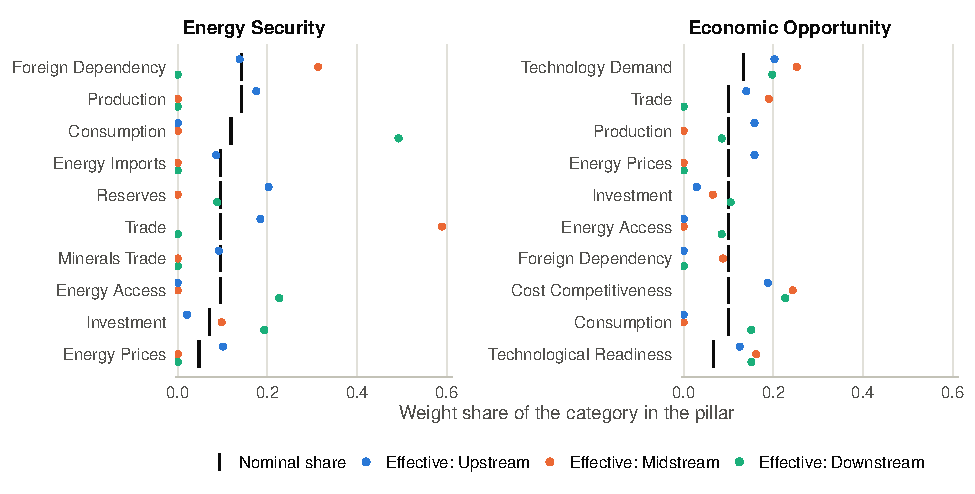
\includegraphics[width=\textwidth]{method_weights}
  \caption{Nominal and effective category weights. Black ticks: nominal share
  $w_k/\sum_{k'}w_{k'}$ over the ten categories of the pillar (\texttt{config/weights.yml};
  Table~\ref{tab:category_weights}). Dots: mean effective weight $\omega_{kits}$
  (equation~\eqref{eq:effective_weight}) over the scored cells of the eleven headline
  technologies at each stage, with $\omega_{kits}=0$ where the category is not observed. A dot
  at zero marks a category that is never observed at that stage. The effective weights of a
  stage, like the nominal shares, sum to one over the categories. A dot to the right of the
  tick means that the available-case rule gives the category more weight than its nominal share.
  Cells: 2,181, 2,002 and 2,049 for $\ES$ and 2,394, 2,346 and 2,391 for $\EO$ (upstream,
  midstream, downstream). Source: category contributions in
  \texttt{data/processed/outputs/index\_outputs.rds}; \texttt{scripts/paper/fig\_method.R}.}
  \label{fig:method_weights}
\end{figure}

% ---------------------------------------------------------------------------
\subsection{Exact decompositions}\label{subsec:norm_decomposition}

With $C_{kits}=\omega_{kits}c_{kits}$ and $\lambda_{vkits}=1/|\mathcal V^{*}_{kits}|$ for a present
component (0 otherwise), every pillar value decomposes exactly into category and variable
contributions,
\begin{equation}\label{eq:cat_decomp}
  \ES_{its}=\sum_{k\in\Cats^{P}}C_{kits},\qquad \sum_{k\in\Cats^{P}}\omega_{kits}=1 ,
\end{equation}
\begin{equation}\label{eq:var_decomp}
  \ES_{its}=\sum_{k\in\Cats^{P}}\sum_{v\in\mathcal V_{k}}
    \underbrace{\omega_{kits}\,\lambda_{vkits}\,\tilde x_{itsv}}_{\text{contribution of }v},
  \qquad
  \sum_{k}\sum_{v}\omega_{kits}\,\lambda_{vkits}=1 .
\end{equation}
The largest absolute difference between the index and the sum of its contributions is exactly
zero for the category decomposition and $1.1\times10^{-16}$ for the variable decomposition, in
both pillars (7,794 $\ES$ and 7,661 $\EO$ cells, all technologies), so the attributions of
Sections~\ref{sec:es} and~\ref{sec:eo} are exact.

% ---------------------------------------------------------------------------
\subsection{The imputed weight share}\label{subsec:norm_diagnostics}

The share of a cell's weight carried by imputed components is
\begin{equation}\label{eq:imputed_share}
  \iota_{its}=\sum_{k}\sum_{v}\omega_{kits}\,\lambda_{vkits}\,
    \1\bigl[\tilde x_{itsv}\text{ imputed}\bigr]\in[0,1],
\end{equation}
counting zero and average fills alike; a world-level series copied to every economy counts as
observed. Imputed components carry on average 31 percent of the weight of an $\ES$ cell and 43
percent of an $\EO$ cell (medians 0.26 and 0.44; Figure~\ref{fig:method_imputation}). The $\ES$
burden is heaviest upstream (0.41, against 0.23 and 0.27), where Reserves, zero-filled for
economies absent from the registers, is imputed at 0.84; the $\EO$ burden is flat across stages
(0.41, 0.44, 0.43). No $\ES$ cell and 24 $\EO$ cells (the Isle of Man 14, Puerto Rico 8,
Liechtenstein 2) rest entirely on imputation. All 30 $\ES$ and 33 $\EO$ headline pairs vary across
economies.

\begin{figure}[tbp]
  \centering
  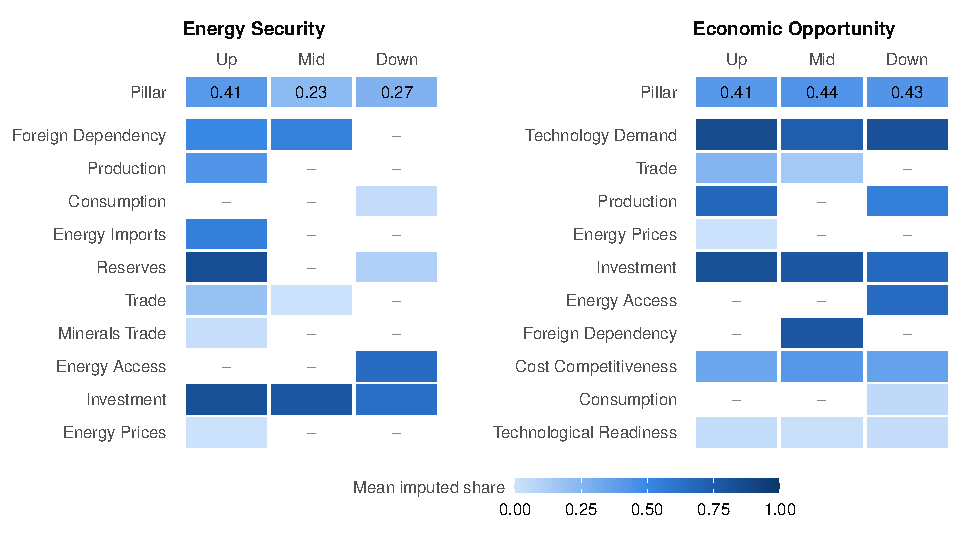
\includegraphics[width=\textwidth]{method_imputation}
  \caption{Imputation burden by category and stage. Category rows: the mean, over the headline
  cells in which the category is observed, of the share of the category score carried by
  imputed components, $\sum_v\lambda_{vkits}\1[\tilde x_{itsv}\text{ imputed}]$. Pillar row
  (with values): the mean imputed weight share $\iota_{its}$ of
  equation~\eqref{eq:imputed_share} over all scored cells of the stage, which weights the
  category rows by the effective weights. Dashes mark categories that are not observed at a
  stage. A component counts as imputed when a missing-data rule of
  Table~\ref{tab:missing_rules} supplied it, zero fills included; world-level series copied to
  every economy count as observed. Online Appendix~\ref{oa:normalization} tabulates the values.
  Source: variable contributions and pillar diagnostics in
  \texttt{data/processed/outputs/index\_outputs.rds}; \texttt{scripts/paper/fig\_method.R}.}
  \label{fig:method_imputation}
\end{figure}

% ---------------------------------------------------------------------------
\subsection{The rankability rule}\label{subsec:norm_rankability}

Every cell the sources reach is scored and enters the decompositions, but a cell enters a
cross-country ranking, a top-$N$ list or the Strategic Index only if it is rankable,
\begin{equation}\label{eq:rankable}
  R_{its}=\1\bigl[i\in\Countries^{\mathrm{sov}}\bigr]\;\1\bigl[\iota_{its}\le\tau\bigr],
  \qquad \tau=0.5 ,
\end{equation}
where $\Countries^{\mathrm{sov}}$ is the set of 195 sovereign states of the Correlates of War
state-system list \citep{cow2024state} (the 193 UN members, Kosovo and Taiwan). The threshold
reads as ``observed data carry at least half of the cell's weight''; values are never altered,
and the Partnership Strength Index applies the same rule to partners (Section~\ref{sec:bilateral}).

Of the 6,232 headline $\ES$ cells, 4,163 (67 percent) are rankable, 607 belonging to territories
and 1,462 to sovereign states over the threshold; in $\EO$, 4,301 of 7,131 (60 percent), with 718
and 2,112 excluded (Figure~\ref{fig:method_rankability}). The rule bites hardest in upstream $\ES$
(52 percent rankable, against 70 and 80), where the registers cover a minority of economies, and
in midstream and downstream $\EO$ (56 and 55 percent, against 70). Every sovereign state keeps a
rankable $\ES$ cell, but 17 keep no rankable $\EO$ cell (Liechtenstein, Monaco and fifteen small
island and low-income states). The rule is not level-neutral: since absence from a register scores
at the bottom, excluded cells lean insecure. Of the 5,854 candidate Strategic Index cells, the
3,154 kept have a mean security need $1-\ES$ of 0.58 and $\EO$ of 0.49, against 0.68 and 0.44 for
those removed. The rule states what the data can support rather than correcting the index;
Section~\ref{sec:robustness} reports other thresholds.

\begin{figure}[tbp]
  \centering
  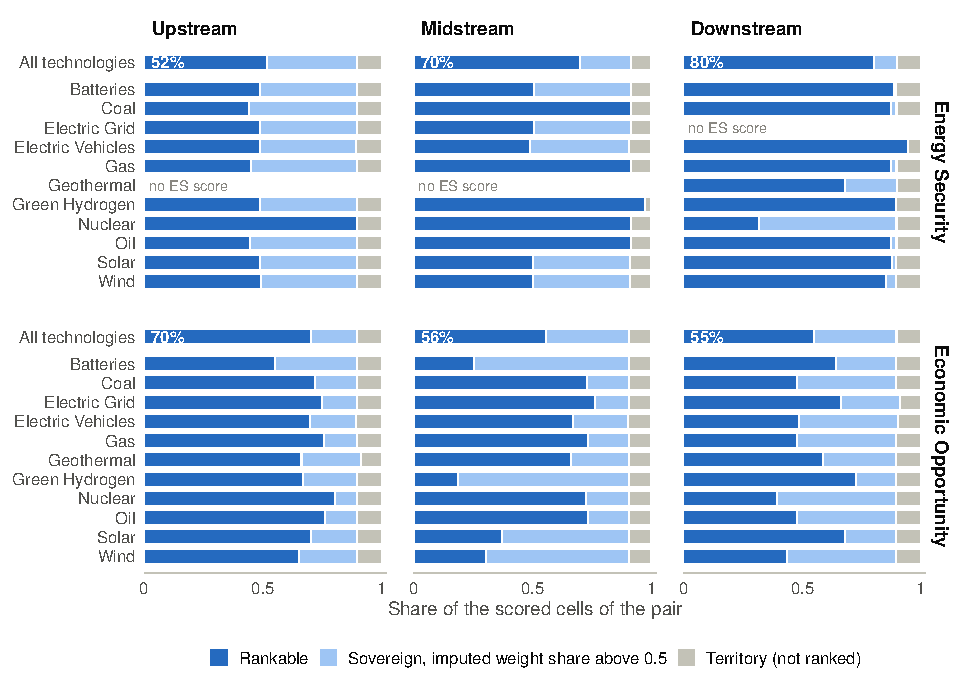
\includegraphics[width=\textwidth]{method_rankability}
  \caption{Rankability of the scored cells by technology--stage pair. Each bar divides the scored
  country--technology--stage cells of a pair into three exclusive groups: rankable cells (the
  economy is a sovereign state and the imputed weight share $\iota_{its}$ is at most
  $\tau=0.5$); cells of sovereign states with $\iota_{its}>0.5$; and cells of territories,
  special administrative regions and the West Bank and Gaza, which are scored but never ranked
  whatever their imputed share. The ``All technologies'' row pools the pairs of the stage, and its
  label gives the rankable share. Sovereignty follows the Correlates of War state-system list (195
  states: the 193 members of the United Nations, Kosovo and Taiwan). ``No ES score'' marks the
  three pairs without an $\ES$ value. Sample: the eleven headline technologies, 6,232 $\ES$ and
  7,131 $\EO$ cells; Online Appendix~\ref{oa:normalization} gives the counts by stage. Source:
  \texttt{energy\_security\_index} and \texttt{economic\_opportunity\_index} in
  \texttt{data/processed/outputs/index\_outputs.rds}; \texttt{config/rankability.yml};
  \texttt{scripts/paper/fig\_method.R}.}
  \label{fig:method_rankability}
\end{figure}

\paragraph{What the construction does not do.} The stages of a technology are scored
independently, although disruptions propagate along supply chains \citep{carvalho2021supply};
dependence across stages enters only where a variable encodes it, as the mineral-supply terms of
foreign dependency do. Section~\ref{sec:robustness} reports the test of vertical complementarities
behind this choice. Imputation assigns one value per uncovered economy, so it understates the
uncertainty of imputed cells.

% =============================================================================
% Section 5. The Energy Security Index
% Specification: R/indices/build_energy_security_index_v2.R, R/indices/index_builder_core.R,
% the ES theme builders in R/categories/** as called from scripts/10_build_themes.R,
% config/weights.yml (energy_security), config/missing_data.yml, config/rankability.yml,
% docs/methodology.md section 4. Results: paper/results/es.json, scripts/paper/fig_es.R (final
% rerun of 2026-10-12). Further results: Online Appendix (sections/oa_es.tex, oa:es);
% variable inventory: Appendix A.
% =============================================================================
\section{The Energy Security Index}\label{sec:es}\label{sec:energy_security}

The Energy Security pillar $\ES_{its}$ asks how far economy $i$ can rely on the supply of
technology $t$ at supply-chain stage $s$: of the minerals it is built from, of the materials,
components and equipment that embody it, and of the energy it delivers. Following
\citet{cherp2014concept}, security is the low vulnerability of vital energy systems, scored on the
dimensions the measurement literature shares: domestic resources, dependence on imports and on few
suppliers, price stability and access
\citep{kruyt2009indicators,sovacool2011conceptualizing,winzer2012conceptualizing,ang2015energy}; in
the terms of \citet{cherp2011three}, sovereignty, resilience and robustness. Because the ``fuel'' of
a clean technology is a bundle of minerals and manufactured inputs, the pillar borrows the
supply-risk logic of the criticality literature
\citep{graedel2012methodology,nassar2020evaluating,kowalski2023raw,iea2025gcmo} and the
concentration index of \citet{hirschman1945national}. A higher score means a more secure position;
the Strategic Index (Section~\ref{sec:strategic}) uses the need $1-\ES_{its}$.

% -----------------------------------------------------------------------------
\subsection{Construction}\label{subsec:es_aggregation}

Ten categories (Table~\ref{tab:es_structure}, weights summing to 42) are combined by the rules of
Section~\ref{sec:normalization} into the available-case weighted mean of
equation~\eqref{eq:pillar}. Registers of holders, producers, exporters or investors carry the zero
rule and the zero-anchored S-curve of equation~\eqref{eq:scurve_zero}, the other themes the
global-average rule (Table~\ref{tab:missing_rules}). The category bundle, and with it the effective
weights of equation~\eqref{eq:effective_weight}, differs across pairs but is common to all
economies within one. Mineral-level terms are aggregated to a technology with demand weights from
the IEA Critical Minerals Dataset \citep{iea2026cmdata}, Stated Policies scenario:
\begin{equation}\label{eq:es_demand_weights}
  w^{y}_{mt}=\frac{D^{y}_{mt}}{\sum_{t'}D^{y}_{mt'}},\qquad
  \tilde w^{y}_{mt}(M)=\frac{w^{y}_{mt}}{\sum_{m'\in M}w^{y}_{m't}},\qquad m\in M,
\end{equation}
where $D^{y}_{mt}$ is the demand for mineral $m$ from application $t$ in the base year $y_0=2025$
or the horizon $y_1=2035$, and $\tilde w$ renormalizes over the set $M$ of minerals a category
observes: $t$'s share of the mineral's clean-energy demand.

\begin{table}[tbp]
\centering
\begin{threeparttable}
\caption{Structure of the Energy Security pillar}
\label{tab:es_structure}
\scriptsize
\setlength{\tabcolsep}{3pt}
\begin{tabularx}{\textwidth}{@{}>{\raggedright\arraybackslash}p{2.1cm}
  >{\raggedright\arraybackslash}p{2.6cm}
  >{\raggedright\arraybackslash}X
  >{\raggedright\arraybackslash}p{2.6cm}
  >{\raggedright\arraybackslash}p{0.9cm}@{}}
\toprule
Category (weight) & Stages: technologies & Components & Sources & Rule\\
\midrule
Foreign Dependency (6) & Up, Mid: Bat, EV, Grid, H$_2$, Sol, Wind &
own share and $1-\HHI$ of mined (Up) or refined (Mid) mineral supply, 2025 and 2035; Mid: share
of world manufacturing capacity (Bat, Sol, Wind), regional EV position (EV) &
IEA Critical Minerals Dataset; IEA ETP; IEA Global EV Outlook & avg, zero\\
Energy Imports (4) & Up: Oil, Gas, Coal & production balance (EJ) and self-sufficiency &
EI Statistical Review; EIA & avg\\
Reserves (4) & Up: all but Geo; Down: Sol, Wind, Geo &
proved fossil reserves; demand-weighted mineral reserves; identified uranium resources;
renewable resource potential &
EI; USGS MCS 2026; Red Book; resource atlases & zero, avg\\
Trade (4) & Up, Mid: all but Geo, H$_2$ &
share of world basket exports; net basket imports/GDP; $1-$ world export
$\HHI^{\dagger}$ & Atlas; UN Comtrade; WDI & avg\\
Minerals Trade (4) & Up: Bat, EV, Grid, H$_2$, Sol, Wind &
demand-weighted share of world mineral exports; $1-\HHI^{\dagger}$ & UN Comtrade & zero\\
Production (6) & Up: Bat, EV, Grid, H$_2$, Sol, Wind, Nuc & demand-weighted mine production;
uranium mine output & EI; Red Book & zero\\
Energy Access (4) & Down: Coal, Oil, Gas, Sol, Wind, Nuc & energy supply per capita, level and
growth & EI & avg\\
Consumption (5) & Down: all but EV, Grid & installed capacity per capita, level and growth to 2035
& BNEF NEO 2024 & avg\\
Energy Prices (2) & Up: all but Geo & commodity price volatility$^{\dagger}$ & IMF PCPS & avg\\
Investment (3) & Up: Bat, EV; Mid: Bat, EV, Sol, Wind; Down: monitor technologies & investment,
momentum, operating and pipeline capacity & Clean Investment Monitor & zero\\
\bottomrule
\end{tabularx}
\begin{tablenotes}[flushleft]\footnotesize
\item \textit{Notes:} Weights from \texttt{config/weights.yml}, renormalized over the observed
categories of each cell (equation~\eqref{eq:pillar}). Up, Mid, Down: upstream, midstream,
downstream; Bat batteries, EV electric vehicles, Grid electric grid, H$_2$ green hydrogen, Sol
solar, Nuc nuclear, Geo geothermal. $^{\dagger}$Constant across economies within a pair. Rule:
missing-data rule of the themes (avg: global average; zero). Variables in
Appendix~\ref{app:variables}.
\end{tablenotes}
\end{threeparttable}
\end{table}

% -----------------------------------------------------------------------------
\subsection{Categories}\label{subsec:es_categories}

\paragraph{Foreign Dependency.}\label{subsec:es_fd} The core component is the economy's position in
the IEA's mined (upstream) and refined (midstream) supply of copper, cobalt, lithium, nickel,
graphite and the magnet rare earths. With $Q^{y}_{ims}$ the supply of mineral $m$ by economy $i$ at
stage $s$,
\begin{align}
  \sigma^{y}_{ims}&=\frac{Q^{y}_{ims}}{\sum_{j}Q^{y}_{jms}},\qquad
  \HHI^{y}_{ms}=\sum_{j}\big(\sigma^{y}_{jms}\big)^{2},\label{eq:es_fd_share}\\
  q_{imts}&=\tfrac14\Big(\Scurve^{0}[\sigma^{y_0}]_{s}+\Scurve^{0}[\sigma^{y_1}]_{s}
  +\Scurve[1-\HHI^{y_0}]_{s}+\Scurve[1-\HHI^{y_1}]_{s}\Big),\label{eq:es_fd_mineral}\\
  \mathrm{MS}_{its}&=\frac{\sum_{m}w^{y_1}_{mt}\,q_{imts}}{\sum_{m}w^{y_1}_{mt}}.
  \label{eq:es_fd_ms}
\end{align}
A non-supplier scores zero on the shares but keeps the concentration terms. Midstream, the
category adds the share of world manufacturing capacity including announced projects for
batteries, solar and wind \citep{iea2024etp}, over the world total including the source's residual
row, and four indices of the EV position of the economy's IEA region. The IEA reports the European
Union as one region, so every EU member carries the EU's 2035 share (0.15 in wind, 0.11 in
batteries, 0.00 in solar) and members are not ranked apart on it.

\paragraph{Energy Imports.}\label{subsec:es_imports} For oil, gas and coal upstream, with production
$P_{if}$ and consumption $C_{if}$ of fuel $f$ in exajoules,
\begin{equation}\label{eq:es_imports}
  B_{if}=P_{if}-C_{if},\qquad \beta_{if}=100\,\frac{P_{if}}{C_{if}},\qquad
  \mathrm{EI}_{if}=\tfrac12\Big(\Scurve[\beta]_{f}+\Scurve[B]_{f}\Big),
\end{equation}
the net balance and self-sufficiency, ranked within the fuel, from the Statistical Review for 2025
\citep{ei2026statistical}. Where it lists no production for an economy and fuel, production is
taken from the EIA's International Energy Statistics \citep{eia2026international}, counted as
observed and paired with consumption of the same year; Estonian coal, for which the Statistical
Review counts oil shale, remains missing.

\paragraph{Reserves.}\label{subsec:es_reserves} Upstream, the category ranks proved oil, gas and
coal reserves (end-2020, the last year the Energy Institute publishes them), reserves of nine
critical minerals from the USGS Mineral Commodity Summaries 2026 (end-2025, with the erratum that
puts Brazil's rare earths at 11\,Mt) \citep{usgs2026mcs}, and identified recoverable uranium
resources below USD 260/kgU from the OECD-NEA/IAEA Red Book \citep{oecdnea2026uranium}. With
$\rho_{im}$ the zero-anchored index of mineral $m$, zero for an unlisted holder,
\begin{equation}\label{eq:es_reserves}
  R_{it}=\Scurve^{0}\Big[\textstyle\sum_{m\in M_t}\tilde w^{y_0}_{mt}(M_t)\,\rho_{im}\Big]_{t},
\end{equation}
so a holder of one mineral does not score that mineral's rank for the whole technology. Holders
the USGS lists without a figure (not available, withheld or small) count as zero. Downstream, the
category scores solar, wind and geothermal resource potential.

\paragraph{Trade.}\label{subsec:es_trade} The crosswalk of Section~\ref{subsec:data_crosswalk}
assigns each pair a basket of HS six-digit products $G_{ts}$: nine midstream baskets and, upstream,
the raw materials of batteries, electric vehicles (battery-mineral ores and magnet rare earths), wind
(rare earths), solar (silicon metal), nuclear (uranium ores and natural uranium compounds), the
fossil fuels and the grid, whose basket holds copper and aluminium inputs rather than electricity.
The category is
\begin{equation}\label{eq:es_trade}
  c_{\mathrm{T},its}=\mean\Big\{\Scurve[-\HHI_{ts}],\
  \Scurve\Big[\tfrac{\sum_{h\in G_{ts}}X_{ih}}{\sum_{h\in G_{ts}}W_{h}}\Big]_{ts},\
  \Scurve\Big[-\tfrac{\sum_{h\in G_{ts}}(M_{ih}-X_{ih})}{\mathrm{GDP}_i}\Big]_{ts}\Big\}:
\end{equation}
the share of world basket exports and net basket imports relative to GDP, from the Atlas of
Economic Complexity \citep{growthlab2019trade,hausmann2014atlas} and WDI \citep{worldbank2026wdi},
and the concentration of world basket exports among UN Comtrade reporters in 2024
\citep{uncomtrade}, which excludes Hong Kong as a re-export hub and is ranked across the 18 basket
cells of the headline technologies. That term takes one value per pair, so it moves the pair's
level without reordering its economies.

\paragraph{Minerals Trade and Production.}\label{subsec:es_minerals_trade}\label{subsec:es_production}
Minerals Trade averages the demand-weighted zero-anchored shares of world exports of the
technology's minerals (for a non-reporter, partners' reported imports converted from CIF to FOB)
with a pair-constant concentration term. Production ranks mine output like reserves,
\begin{equation}\label{eq:es_production}
  \mathrm{P}_{it}=\Scurve^{0}\Big[\textstyle\sum_{m\in M_t}\tilde w^{y_0}_{mt}(M_t)\,\pi_{im}\Big]_{t},
\end{equation}
and, for nuclear, uranium mine output from the Red Book. Fossil output enters only through Energy
Imports.

\paragraph{Energy Access, Consumption, Prices and Investment.}\label{subsec:es_access}%
\label{subsec:es_consumption}\label{subsec:es_prices}\label{subsec:es_investment}
Downstream, Energy Access ranks energy supply per capita in 2025 and its growth since 2020, by
fuel; Consumption ranks installed capacity per capita in 2024 and its projected growth to 2035
\citep{bnef2024neo}. Both read a deeper, expanding domestic system as more secure; treating high
use as exposure would reverse the sign (Section~\ref{subsec:eo_shared}). Energy Prices is
$\Scurve[-\bar v_t]$, with $\bar v_t$ the mean annualized volatility of monthly log changes in the
technology's IMF commodity prices over 1, 5, 10 and 20 years \citep{imf2026pcps}, a world value.
Investment ranks clean-technology investment, its three-year momentum, and operating and pipeline
manufacturing capacity \citep{cim2026}; upstream critical-minerals investment is split between
batteries and electric vehicles by their IEA demand shares, 11.5 and 88.5 per cent.

% -----------------------------------------------------------------------------
\subsection{Results}\label{subsec:es_results}

\paragraph{Coverage.} The pillar scores 6{,}232 cells of the eleven headline technologies for 219
economies (195 sovereign, 24 territories) in 30 of the 33 pairs (Geothermal upstream and midstream
and Electric Grid downstream have no category). No pair is constant and no cell fully imputed; the
mean imputed weight share is 0.41, 0.23 and 0.27 by stage. All rankings and summaries use the 4{,}163 rankable cells
(Section~\ref{subsec:norm_diagnostics}): 1{,}124 of 2{,}181 upstream, where the world price series
places every economy in each pair while the mineral and fossil sources cover far fewer, 1{,}397 of
2{,}002 midstream and 1{,}642 of 2{,}049 downstream.

\paragraph{Distribution.} The median rankable cell scores 0.28 upstream (interquartile range 0.19
to 0.37), 0.46 midstream (0.36 to 0.53) and 0.44 downstream (0.35 to 0.52), with a right-skewed
upstream distribution (Figure~\ref{fig:es_distribution}): in the median upstream pair 71 per cent
of rankable economies score zero on Reserves and 84 per cent on Production. Technology-stage fixed
effects explain 44 per cent of the variance, country effects alone 12 per cent and both together
60 per cent (28 per cent of the within-pair variance), and the pair effects reflect the category
bundles rather than the cell-constant inputs. Rankings are meaningful within a pair; comparing one
economy's levels across pairs, as the Strategic Index does, mixes content with construction.

\begin{figure}[tbp]
  \centering
  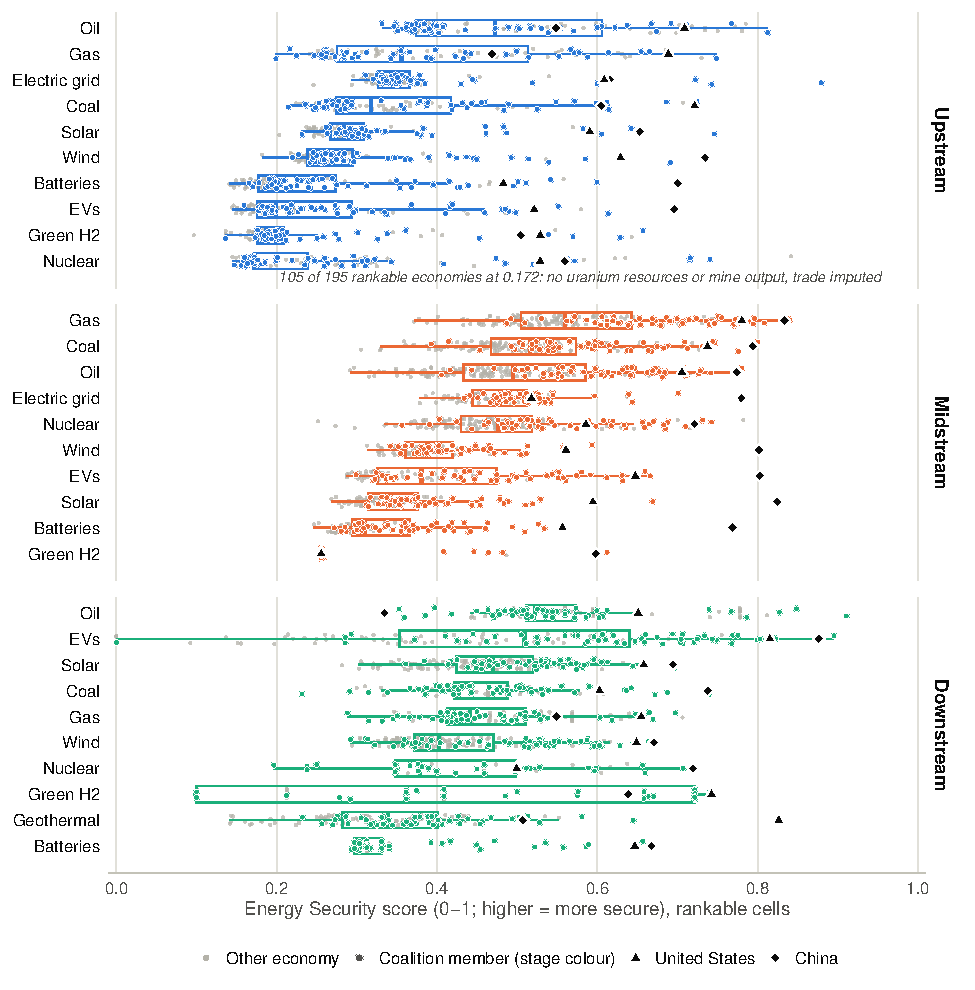
\includegraphics[width=\textwidth]{es_distribution}
  \caption{Energy Security by technology and stage, rankable cells (68 to 195 economies per
  pair; sovereign economy with at most half of the index weight imputed). Boxes span the
  interquartile range; gray dots are non-members, coloured dots coalition members in the stage
  colour; the triangle marks the United States and the diamond China. In Nuclear upstream, 105 of
  the 195 economies, which have neither uranium resources, production nor observed uranium trade,
  share the value 0.172 (Energy Prices plus an imputed Trade category). In Green Hydrogen
  midstream 90 per cent of economies share 0.26. Source: \texttt{energy\_security\_index} in
  \texttt{index\_outputs.rds}, final run; \texttt{scripts/paper/fig\_es.R}.}
  \label{fig:es_distribution}
\end{figure}

\paragraph{Drivers.} The exact category decomposition (equation~\eqref{eq:cat_decomp},
Figure~\ref{fig:es_category_contrib}) shows that upstream Trade supplies 31 per cent of the average
score, Energy Prices 20, Minerals Trade 16 and Foreign Dependency 13, while Reserves and Production
supply 7.2 and 3.1 per cent against mean effective weights of 20 and 19.5 per cent: for the typical
economy the registers add nothing, for the few holders they decide the top. Midstream, Trade
supplies 73 per cent and Foreign Dependency 26; downstream, Consumption 56 and Energy Access 24.
The cell-constant inputs carry a mean effective weight of 0.21 upstream and 0.22 midstream but
supply 36 and 26 per cent of the score. Reserves and Production correlate at a within-pair median
of 0.84, so upstream the pillar counts mineral endowment twice.

\begin{figure}[tbp]
  \centering
  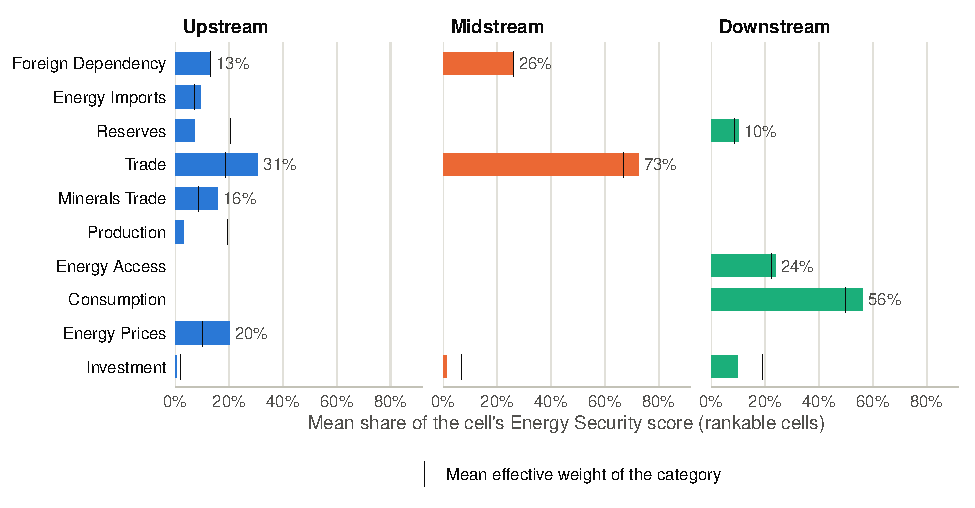
\includegraphics[width=\textwidth]{es_category_contrib}
  \caption{Average composition of Energy Security by stage, rankable cells. Bars: mean share of
  each category in the score, $\omega_{kits}c_{kits}/\ES_{its}$ (equation~\eqref{eq:cat_decomp});
  ticks: the category's mean effective weight. A bar much shorter than its tick, as for Reserves
  and Production upstream, marks a category on which most economies score zero. The upstream
  Energy Prices and Trade shares include Nuclear upstream (15 and 28 per cent without it). Sample:
  1{,}124 upstream, 1{,}397 midstream and 1{,}637 downstream cells. Source:
  \texttt{energy\_security\_outputs\$category\_contributions}; \texttt{scripts/paper/fig\_es.R}.}
  \label{fig:es_category_contrib}
\end{figure}

\paragraph{Uranium.} Nuclear upstream is scored on Energy Prices, Trade, Reserves and Production,
with effective weights of 1/8, 1/4, 1/4 and 3/8 (Figure~\ref{fig:es_nuclear_upstream}). Of the 195
rankable economies, 58 hold identified resources and 18 of them produce. The 105 economies with
neither and without observed uranium trade share one value, 0.172; the other 32 without uranium lie
between 0.145 and 0.201. Kazakhstan leads (0.84), ahead of Canada (0.74), Namibia and Australia
(0.72); China is tenth (0.56) and the United States eleventh (0.53); 31 of the 57 coalition members
hold resources. Read as a need, the common value becomes a uniform 0.83 that measures absence
rather than a gap domestic supply could close. Because 86 of the 174 countries with a Strategic
Index share it, the allied picks admit an upstream stage only where the country records reserves
or production of its resources (Section~\ref{subsec:si_allied}), a pick-eligibility rule, not part
of the index.

\begin{figure}[tbp]
  \centering
  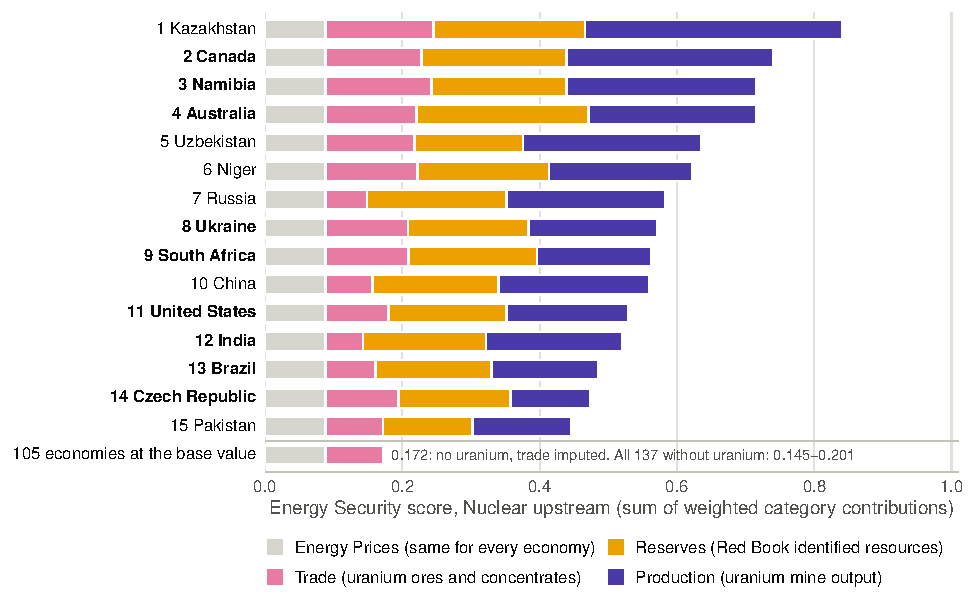
\includegraphics[width=\textwidth]{es_nuclear_upstream}
  \caption{Composition of Energy Security in Nuclear upstream: the 15 highest-ranked of 195
  rankable economies (coalition members in bold), split into Energy Prices (uranium price
  volatility, 0.088 for every economy), Trade (uranium ores, concentrates and natural uranium
  compounds), Reserves (identified resources below USD 260/kgU, OECD-NEA/IAEA Red Book) and
  Production (mine output). The bottom row stands for the 105 economies without uranium whose
  uranium trade is not observed (0.172). Source: \texttt{energy\_security\_index} and its category
  contributions; \texttt{scripts/paper/fig\_es.R}.}
  \label{fig:es_nuclear_upstream}
\end{figure}

\paragraph{Leaders and the coalition.} China leads 11 of the 30 pairs (Table~\ref{tab:es_leaders}):
three upstream mineral pairs, five midstream pairs, through its shares of refined supply and
manufacturing capacity \citep{iea2024etp,iea2025gcmo}, and three downstream pairs; no other
economy leads more than two. Upstream, leadership follows endowments (Saudi Arabia in oil, Qatar in
gas, Kazakhstan in nuclear, Chile in the grid and solar); in Oil upstream China ranks 34th, the
position of an importer (Figure~\ref{fig:es_top}). A coalition member is first in 16 pairs and in
the top three of all 30. The 57 members have mean within-pair percentiles of 0.59, 0.72 and 0.62 by
stage, against 0.47, 0.41 and 0.50 for other economies (Figure~\ref{fig:es_heatmap}); the United
States averages 0.95, China 0.92 (0.99 midstream), and Taiwan has the profile of a manufacturer
without resources (0.75 midstream, 0.01 upstream). Canada is the one high-income member with a
gap in the heatmap: its Downstream Consumption category is imputed at the global average in all
eight cells it enters, because the BloombergNEF outlook behind it neither models Canada nor has a
North American aggregate, so six of its nine scored Downstream cells are not rankable (the other
economies with the whole category imputed are Taiwan, Bermuda and seven South Asian economies). The
lead is unsurprising for a coalition of
large or resource-rich economies; whether members' strengths complement one another is the subject
of Section~\ref{sec:network}. Online Appendix~\ref{oa:es} details the leaders, the tiers and the
category correlations.

% Generated by scripts/paper/fig_es.R; do not edit by hand.
\begin{table}[tbp]
\centering
\begin{threeparttable}
\caption{Leading economies in each technology-stage pair of the Energy Security pillar (rankable cells)}
\label{tab:es_leaders}
\footnotesize
\begin{tabular}{@{}lrlllcrr@{}}
\toprule
Technology & $n$ & First & Second & Third & Best member (rank) & USA & CHN \\
\midrule
\multicolumn{8}{@{}l}{\textit{Upstream}}\\
Batteries & 106 & CHN 0.70 & AUS 0.60 & RUS 0.56 & AUS (2) & 9 & 1 \\
Coal & 96 & AUS 0.72 & USA 0.72 & RUS 0.71 & AUS (1) & 2 & 8 \\
Electric Grid & 106 & CHL 0.88 & COD 0.74 & PER 0.72 & CHL (1) & 5 & 4 \\
Electric Vehicles & 107 & CHN 0.70 & AUS 0.61 & RUS 0.58 & AUS (2) & 5 & 1 \\
Gas & 98 & QAT 0.75 & RUS 0.73 & USA 0.69 & QAT (1) & 3 & 33 \\
Green Hydrogen & 106 & ZAF 0.66 & RUS 0.64 & IDN 0.63 & ZAF (1) & 7 & 8 \\
Nuclear & 195 & KAZ 0.84 & CAN 0.74 & NAM 0.72 & CAN (2) & 11 & 10 \\
Oil & 97 & SAU 0.81 & VEN 0.79 & IRQ 0.78 & SAU (1) & 12 & 34 \\
Solar & 106 & CHL 0.75 & CHN 0.65 & PER 0.64 & CHL (1) & 5 & 2 \\
Wind & 107 & CHN 0.73 & AUS 0.69 & USA 0.63 & AUS (2) & 3 & 1 \\
\addlinespace
\multicolumn{8}{@{}l}{\textit{Midstream}}\\
Batteries & 106 & CHN 0.77 & USA 0.56 & CAN 0.53 & USA (2) & 2 & 1 \\
Coal & 190 & POL 0.80 & MOZ 0.80 & CHN 0.79 & POL (1) & 10 & 3 \\
Electric Grid & 106 & CHN 0.78 & JPN 0.70 & CHL 0.64 & JPN (2) & 22 & 1 \\
Electric Vehicles & 105 & CHN 0.80 & ESP 0.67 & HUN 0.66 & ESP (2) & 4 & 1 \\
Gas & 192 & KOR 0.84 & CHN 0.83 & ITA 0.81 & KOR (1) & 8 & 2 \\
Green Hydrogen & 106 & IDN 0.61 & CHN 0.60 & RUS 0.49 & IDN (1) & 12$^{95}$ & 2 \\
Nuclear & 188 & RUS 0.78 & FRA 0.74 & NLD 0.73 & FRA (2) & 30 & 5 \\
Oil & 192 & KOR 0.78 & CHN 0.77 & GAB 0.74 & KOR (1) & 11 & 2 \\
Solar & 106 & CHN 0.82 & IND 0.67 & USA 0.59 & IND (2) & 3 & 1 \\
Wind & 106 & CHN 0.80 & POL 0.59 & USA 0.56 & POL (2) & 3 & 1 \\
\addlinespace
\multicolumn{8}{@{}l}{\textit{Downstream}}\\
Batteries & 186 & CHN 0.67 & DEU 0.66 & USA 0.65 & DEU (2) & 3 & 1 \\
Coal & 186 & IDN 0.74 & CHN 0.74 & JPN 0.69 & IDN (1) & 9 & 2 \\
Electric Vehicles & 121 & TUR 0.90 & CHN 0.88 & VNM 0.82 & TUR (1) & 4 & 2 \\
Gas & 186 & KWT 0.71 & QAT 0.70 & KOR 0.67 & QAT (2) & 6 & 24 \\
Geothermal & 146 & USA 0.83 & IDN 0.64 & JPN 0.58 & USA (1) & 1 & 9 \\
Green Hydrogen & 186 & USA 0.74 & KOR 0.74 & ALB 0.72$^{49}$ & USA (1) & 1 & 63 \\
Nuclear & 68 & CHN 0.72 & FRA 0.71 & JPN 0.66 & FRA (2) & 17 & 1 \\
Oil & 186 & QAT 0.91 & OMN 0.85 & ARE 0.83 & QAT (1) & 23 & 186 \\
Solar & 191 & SAU 0.70 & AUS 0.70 & CHN 0.69 & SAU (1) & 4 & 3 \\
Wind & 186 & CHN 0.67 & CAN 0.66 & USA 0.65 & CAN (2) & 3 & 1 \\
\bottomrule
\end{tabular}
\begin{tablenotes}[flushleft]\footnotesize
\item \textit{Notes:} $\ES_{its}$ for the eleven headline technologies, final run. Only rankable cells enter: a sovereign economy with at most half of the cell's index weight imputed. Economies are identified by ISO3 code and followed by their score; $n$ is the number of rankable economies in the pair. ``Best member'' is the highest-ranked of the 57 coalition members, with its rank in parentheses; the USA and CHN columns give the ranks of the United States and China. A rank is one plus the number of rankable economies with a strictly higher score, so tied economies share a rank, and a superscript gives the number of economies that share it (the economy listed is the first of them alphabetically). Geothermal upstream, Geothermal midstream and Electric Grid downstream have no Energy Security score. Source: \texttt{energy\_security\_index} in \texttt{index\_outputs.rds}; \texttt{scripts/paper/fig\_es.R}.
\end{tablenotes}
\end{threeparttable}
\end{table}


\begin{figure}[tbp]
  \centering
  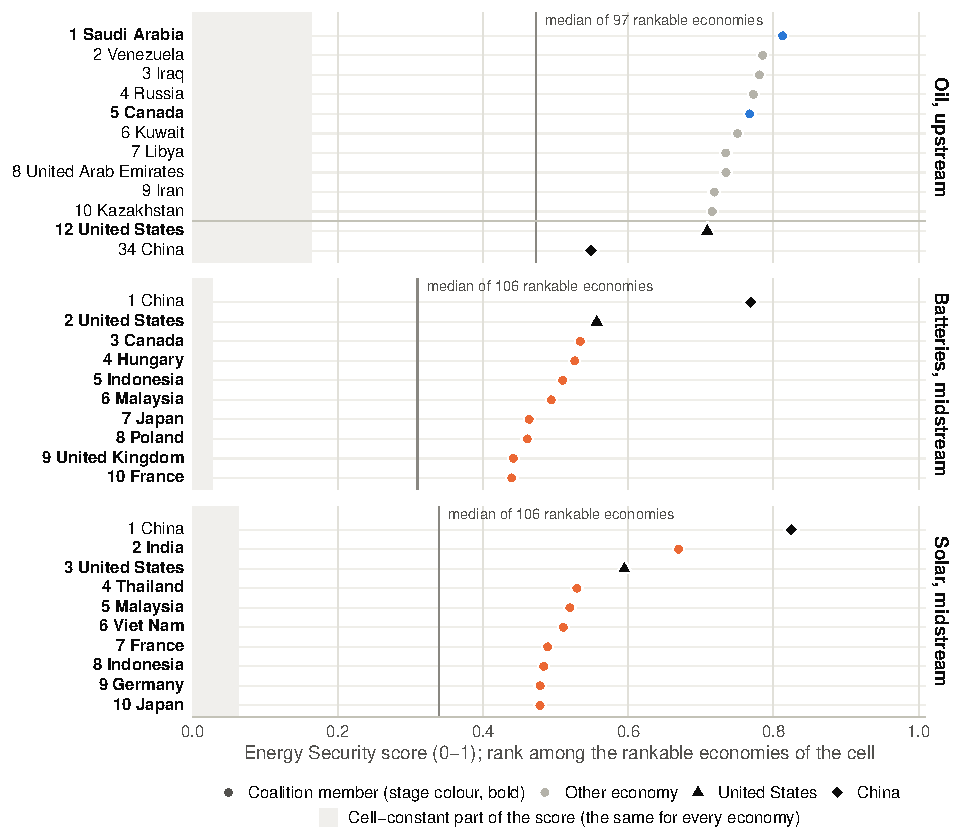
\includegraphics[width=\textwidth]{es_top}
  \caption{The ten highest-ranked economies in Oil upstream, Batteries midstream and Solar
  midstream (97, 106 and 106 rankable economies), with the United States (triangle) and China
  (diamond) appended when outside the top ten. Coalition members are in bold and the stage colour.
  The vertical line is the pair median; the shaded band is the cell-constant part of the score
  (0.16, 0.03 and 0.06). Source: \texttt{energy\_security\_index} and its variable contributions;
  \texttt{scripts/paper/fig\_es.R}.}
  \label{fig:es_top}
\end{figure}

\begin{figure}[tbp]
  \centering
  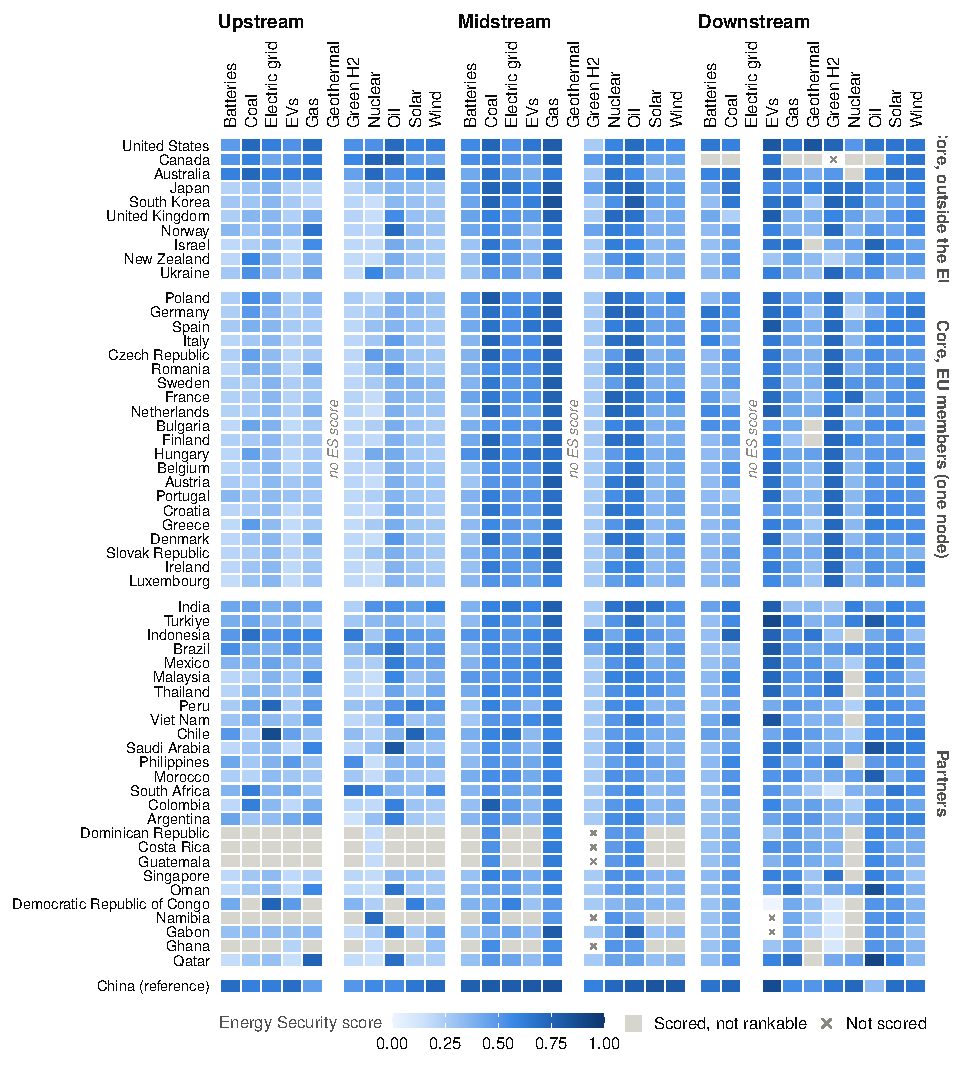
\includegraphics[width=\textwidth]{es_heatmap}
  \caption{Energy Security of the 57 coalition members across the 33 sectors, grouped into the
  ten core members outside the EU, the 21 core EU members and the
  26 partners, each ordered by mean within-pair percentile; China for reference. Colour gives
  $\ES_{its}$ for rankable cells; gray cells are scored but not rankable, crosses unscored, and the
  three sectors without an Energy Security score are blank. Canada's Downstream cells rest on an
  imputed Consumption category (its source, the BloombergNEF outlook, does not report Canada), so six
  of them are not rankable. Source: \texttt{energy\_security\_index}
  and \texttt{coalition\_members}; \texttt{scripts/paper/fig\_es.R}.}
  \label{fig:es_heatmap}
\end{figure}

\paragraph{Caveats.} Several pairs rank few distinct values: in the Strategic Index sample, Green
Hydrogen midstream has 34 of 40 countries at one value, Nuclear upstream 86 of 174, Green Hydrogen
downstream 45 of 158, Nuclear downstream 19 of 67 and Batteries downstream 38 of 138, and under the
need reading each mass point becomes a uniformly high need (Section~\ref{sec:strategic}).
Unquantified holders count as zero, and the downstream reading treats deeper domestic use of a
fossil fuel as security.

% =============================================================================
% Section 6. The Economic Opportunity Index
% Specification: R/indices/build_economic_opportunity_index_v2.R, R/indices/index_builder_core.R,
% the EO theme builders as called from scripts/10_build_themes.R:
%   R/categories/trade/{trade_core,export_feasibility,trade_concentration}.R
%   R/categories/production/production_depth_momentum.R
%   R/categories/technology_demand/{future_demand,overcapacity_premium}.R
%   R/categories/technological_readiness/technological_readiness.R
%     (+ config/iea_clean_tech_guide_tech_map.yml, stage mapping)
%   R/categories/energy_prices/{energy_prices,lcoe_competitiveness}.R
%   R/categories/investment/investment_momentum.R
%   R/categories/energy_access/energy_access_consumption.R, R/categories/consumption/energy_consumption.R
%   R/categories/foreign_dependency/market_share_manufacturing.R
%   R/categories/economic opportunity/cost_competitiveness.R
% config/weights.yml (economic_opportunity), config/missing_data.yml, config/rankability.yml.
% Results: paper/results/eo.json, scripts/paper/fig_eo.R (final rerun of 2026-10-12);
% fig_eo_transforms.R. Further detail: Online Appendix (sections/oa_eo.tex, oa:eo).
% =============================================================================
\FloatBarrier
\section{The Economic Opportunity Index}\label{sec:eo}\label{sec:economic_opportunity}

The Economic Opportunity pillar $\EO_{its}$ asks how well placed economy $i$ is to capture value
from the expansion of technology $t$ at stage $s$. Its premise comes from economic complexity:
countries diversify into activities close, in capability space, to those they already perform
competitively, and relatedness predicts new comparative advantage
\citep{hidalgo2007product,hausmann2006structural,hausmann2014atlas,hidalgo2009building,hausmann2022implied,hidalgo2021economic,hausmann2007what},
including in low-carbon products \citep{mealy2022economic,growthlab2024greenplexity}. We apply it
at the supply-chain stage, where green industrial policy is now designed
\citep{rodrik2014green,juhasz2024new}, and add market size and growth, cost, technological
maturity and committed capital. A higher score means more opportunity; $\EO_{its}$ is not the
complement of $\ES_{its}$ (Section~\ref{subsec:eo_shared}).

% -----------------------------------------------------------------------------
\subsection{Construction}\label{subsec:eo_aggregation}

Ten categories (Table~\ref{tab:eo_structure}) are combined by the rules of
Section~\ref{sec:normalization} into the available-case weighted mean of
equation~\eqref{eq:pillar}. The weights sum to 30: eight categories carry 3, Technology Demand 4
and Technological Readiness 2. $\Scurve[x]_g$ is the S-curve of equation~\eqref{eq:scurve}
($\gamma=0.5$) within comparison set $g$, by default the pair $(t,s)$. Technological Readiness and
the input-cost component of Cost Competitiveness cover all 33 pairs. Technological Readiness,
Energy Prices and three of the four Technology Demand components are constant within a pair: by
equation~\eqref{eq:affine_constant} they shift a pair's level without reordering its economies.
Appendix~\ref{app:variables} lists every variable; Online Appendix~\ref{oa:eo} gives further
detail.

\begin{table}[tp]
\centering
\begin{threeparttable}
\caption{Structure of the Economic Opportunity pillar}
\label{tab:eo_structure}
\scriptsize
\setlength{\tabcolsep}{3pt}
\begin{tabularx}{\textwidth}{@{}>{\raggedright\arraybackslash}p{1.8cm}
  >{\centering\arraybackslash}p{0.9cm}
  >{\raggedright\arraybackslash}X
  >{\raggedright\arraybackslash}p{2.4cm}
  >{\raggedright\arraybackslash}p{2.3cm}
  >{\raggedright\arraybackslash}p{1.2cm}@{}}
\toprule
Category & Weight (share) & Components (stage: technologies) & Sources & Higher score $=$ & Missing rule\\
\midrule
Trade & 3 (0.10) &
Share of world basket exports; Balassa RCA; basket export value; product-space feasibility;
world export concentration$^{\dagger}$ (Up, Mid: all but Geo, H$_2$) &
Atlas HS92; UN Comtrade &
larger, more specialised exports; closer capabilities; contestable market & avg\\
\addlinespace
Production & 3 (0.10) &
Level, absolute change and a composite of fossil output (Up: Oil, Gas, Coal), uranium mine output
(Up: Nuc), demand-weighted share of world mined mineral supply (Up: Bat, EV, Grid, H$_2$, Sol,
Wind) or power generation (Down: Sol, Wind, Nuc, Coal, Gas, Oil) &
EI Statistical Review; EIA; Red Book; IEA Critical Minerals Dataset &
larger, faster-growing production & avg\\
\addlinespace
Technology Demand & 4 (0.13) &
World supply in 2035 and its growth$^{\dagger}$; regional demand (12 economies) or the EV car
market (Down: EV); US addressable market$^{\dagger}$; manufacturing overcapacity$^{\dagger}$ (Mid:
Bat, Sol, Wind, H$_2$) &
IEA WEO 2025; BNEF NEO 2024; IEA GEVO 2026; BCG; BNEF &
larger, faster-growing market; less overcapacity & avg\\
\addlinespace
Technological Readiness & 2 (0.07) &
TRL Index of the items mapped to the technology and stage: bell-shaped level score and capped
momentum$^{\dagger}$ (all pairs) &
IEA Clean Energy Technology Guide &
readiness nearer TRL 6; faster maturation & avg\\
\addlinespace
Energy Prices & 3 (0.10) &
Commodity price volatility$^{\dagger}$ (Up: all but Geo) & IMF PCPS & lower volatility & avg\\
\addlinespace
Investment & 3 (0.10) &
Investment; three-year momentum; operating and pipeline manufacturing capacity (Up: Bat, EV; Mid:
Bat, EV, Sol, Wind; Down: Bat, EV, Geo, Nuc, Sol, Wind) &
Clean Investment Monitor & more investment and capacity & zero\\
\addlinespace
Energy Access & 3 (0.10) &
Energy supply per capita and its 2020--2025 growth (Down: Coal, Oil, Gas, Sol, Wind, Nuc) &
EI Statistical Review & deeper, growing home market & avg\\
\addlinespace
Foreign Dependency & 3 (0.10) &
Share of world manufacturing capacity incl.\ pipeline (Mid: Bat, Sol, Wind, H$_2$); regional EV
production position (Mid: EV) &
IEA ETP; IEA EV data & larger share of world manufacturing & zero\\
\addlinespace
Cost Competitiveness & 3 (0.10) &
LCOE Index (Down: Bat, Coal, Gas, Sol, Wind); Input Cost Index of wages and capital costs (all
pairs); relative equipment cost (Mid: Bat, Sol, Wind, H$_2$; Down: H$_2$) &
BNEF; ILOSTAT; IMF; IEA & lower costs & none (LCOE); avg\\
\addlinespace
Consumption & 3 (0.10) &
Installed capacity per capita and its growth to 2035 (Down: all but EV, Grid) &
BNEF NEO 2024 & deeper installed base & avg\\
\bottomrule
\end{tabularx}
\begin{tablenotes}[flushleft]\footnotesize
\item \textit{Notes:} Weights from \texttt{config/weights.yml}; shares $w_k/30$ apply where every
category is observed (equation~\eqref{eq:pillar}). Abbreviations as in Table~\ref{tab:es_structure}.
$^{\dagger}$Constant across economies within a pair. Missing rules from
\texttt{config/missing\_data.yml} (Table~\ref{tab:missing_rules}); ``avg'' is the global-average
rule.
\end{tablenotes}
\end{threeparttable}
\end{table}

% -----------------------------------------------------------------------------
\subsection{Categories}\label{subsec:eo_categories}

\paragraph{Trade.}\label{subsec:eo_trade} Trade measures revealed and latent capability to export
the goods of a stage, using the baskets $G_{ts}$ of Section~\ref{subsec:data_crosswalk}; the
upstream baskets give every upstream pair except Geothermal and Green Hydrogen a Trade category. Besides the Atlas
share of world basket exports \citep{growthlab2019trade}, shared with ES, it ranks revealed
comparative advantage \citep{balassa1965trade} from UN Comtrade \citep{uncomtrade},
\begin{equation}\label{eq:eo_rca}
  \RCA_{its}=\frac{E_{its}/T_i}{\sum_{j\in R}E_{jts}\big/\sum_{j\in R}T_j},
\end{equation}
with $E_{its}$ basket and $T_i$ total exports over the reporters $R$; the value of basket exports
$E$; and latent capability, the mean Atlas distance $\delta_{i\eta}$ to the basket's HS four-digit
headings $\mathcal H_{ts}$ \citep{hidalgo2007product},
\begin{equation}\label{eq:eo_feas}
  \mathrm{feas}_{its}=1-\frac{1}{|\mathcal H_{ts}|}\sum_{\eta\in\mathcal H_{ts}}\delta_{i\eta}.
\end{equation}
The fifth component is the world-market concentration term of the ES category, read as
contestability. Then
\begin{equation}\label{eq:eo_trade}
  c_{\mathrm{T},its}=\mean\Big\{\Scurve[\mathrm{ms}]_{ts},\ \Scurve[\RCA]_{ts},\
  \Scurve[E]_{ts},\ \Scurve[\mathrm{feas}]_{ts},\ \Scurve[-\HHI]\Big\}.
\end{equation}
Hong Kong, a re-export hub, is excluded from the Comtrade measures (RCA, export value,
concentration) but keeps its Atlas components, and the concentration term is ranked across the
cells of the eleven headline technologies.

\paragraph{Production.}\label{subsec:eo_production} Production measures the depth of existing
output and its momentum. For oil, gas, coal and uranium upstream and electricity generation
downstream, with output $P_{it,y}$ from the Statistical Review \citep{ei2026statistical} (filled
from EIA where it lists none, Section~\ref{subsec:es_imports}) or the Red Book, and relative and
absolute changes $g^{\mathrm{rel}}$, $g^{\mathrm{abs}}$ over five years,
\begin{equation}\label{eq:eo_prod_energy}
  \mathrm{size}_{its}=\Scurve[P_{\cdot,2025}]_{ts},\qquad
  \mathrm{gabs}_{its}=\Scurve[g^{\mathrm{abs}}]_{ts},\qquad
  O_{its}=\Scurve\Big[\tfrac13\big(\Scurve[P_{\cdot,2025}]+\Scurve[g^{\mathrm{rel}}]
  +\Scurve[g^{\mathrm{abs}}]\big)\Big]_{ts}.
\end{equation}
For the six mineral-intensive technologies upstream, mined supply $S_{im}$ of each mineral in the
IEA base year $y_0$ and in 2035 \citep{iea2026cmdata} enters as a share of base-year world supply
$W_m$, weighted by the technology's demand share $\tilde w_{mt}$:
\begin{equation}\label{eq:eo_prod_mineral}
\begin{gathered}
  s^{y}_{it}=\sum_{m}\tilde w_{mt}\,\frac{S_{im,y}}{W_{m,y_0}},\qquad
  \mathrm{size}_{its}=\Scurve[s^{y_0}]_{ts},\\
  \mathrm{gabs}_{its}=\Scurve[s^{2035}-s^{y_0}]_{ts},\qquad
  O_{its}=\Scurve[2\,\mathrm{size}+\mathrm{gabs}+h_t]_{ts},
\end{gathered}
\end{equation}
so growth is an absolute change in base-year world-share units and $h_t$ is a concentration term
common to the pair. In every cell $c_{\mathrm{P},its}=\tfrac13(\mathrm{size}+\mathrm{gabs}+O)$.

\paragraph{Technology Demand.}\label{subsec:eo_demand} Four sources each contribute one composite.
Two energy outlooks weight growth twice as heavily as size:
\begin{align}
  \mathrm{GD}_{t}&=\Scurve\Big[\tfrac13\big(\Scurve[D_{\cdot,2035}]+2\,\Scurve[D_{\cdot,2035}-D_{\cdot,2024}]\big)\Big],
  \label{eq:eo_weo}\\
  \mathrm{RD}_{it}&=\Scurve\Big[\tfrac13\big(\Scurve[D_{\cdot t,2035}]_t
  +2\,\Scurve\big[D_{\cdot t,2035}/D_{\cdot t,2024}-1\big]_t\big)\Big]_t ,
  \label{eq:eo_bnef}
\end{align}
where $D_{f,y}$ is world supply of fuel $f$ in the World Energy Outlook's Stated Policies Scenario
\citep{iea2025weo}, ranked across seven fuels, and $D_{it,y}$ primary energy consumption in the
twelve economies BloombergNEF models \citep{bnef2024neo}; downstream electric vehicles use the EV
market composite of the Global EV Outlook \citep{iea2026gevo} instead. The third source is BCG's
US serviceable addressable market, one value per pair; the fourth is midstream overcapacity, with
$\rho_t$ the ratio of manufacturing capacity to forecast demand in BloombergNEF's supply-chain data,
\begin{equation}\label{eq:eo_overcap}
  \mathrm{OV}_t=2^{-\rho_t},
\end{equation}
so that capacity equal to demand scores $1/2$ and each further multiple halves the score
(Figure~\ref{fig:eo_transforms}c). Then
\begin{equation}\label{eq:eo_demand}
  c_{\mathrm{TD},its}=\mean\big\{\mathrm{GD}_t,\ \mathrm{RD}_{it},\
  \Scurve[\mathrm{SAM}]_{ts},\ \mathrm{OV}_t\big\}.
\end{equation}

\paragraph{Technological Readiness.}\label{subsec:eo_trl} Opportunity is taken to be greatest
around the demonstration stage, where learning is fast and first-mover positions are open. The
IEA Clean Energy Technology Guide \citep{iea2026cleantechguide} grades technology designs by
readiness level (TRL) for 2020--2025; its post-TRL-9 adoption stages are read as levels 9 to 11.
Ordered rules map each item to a technology and a stage, and a stage without items takes the
technology-wide value. For item $n$ with level $x_n$ and change $\Delta_n$,
\begin{equation}\label{eq:eo_trl_bell}
  b(x)=\begin{cases}
    0, & x\le 2\ \text{or}\ x\ge 11,\\[2pt]
    \cos\!\big(\tfrac{\pi}{2}\,\tfrac{6-x}{4}\big), & 2<x\le 6,\\[4pt]
    \cos\!\big(\tfrac{\pi}{2}\,\tfrac{x-6}{5}\big), & 6<x<11,
  \end{cases}
  \qquad
  \psi(\Delta)=\Big(\frac{\min\{\max\{\Delta,0\},3\}}{3}\Big)^{1/2},
\end{equation}
\begin{equation}\label{eq:eo_trl}
  \mathrm{TRL}_{ts}=\frac{1}{|N_{ts}|}\sum_{n\in N_{ts}}\big[0.7\,b(x_n)+0.3\,\psi(\Delta_n)\big],
\end{equation}
a cardinal index constant within a pair but different across a technology's stages. Of the
Guide's 634 items, 253 map to a headline technology; the index runs from 0.31 (Geothermal
downstream) to 0.72 (Gas downstream).

\begin{figure}[t]
  \centering
  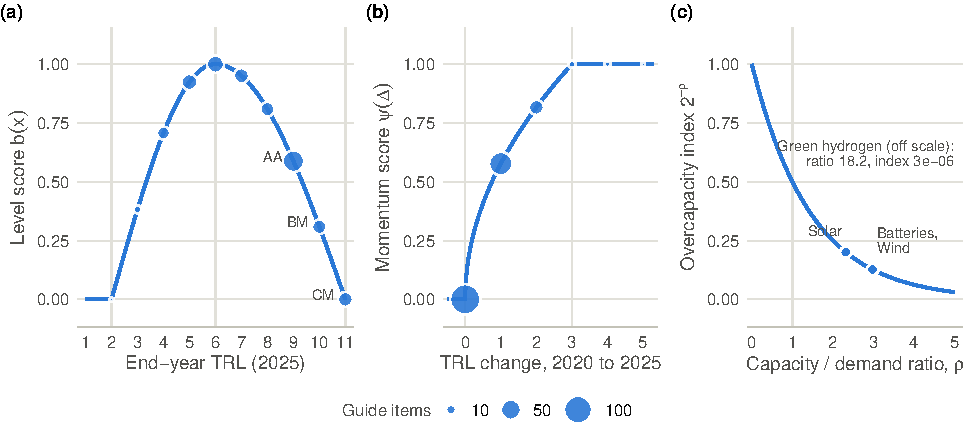
\includegraphics[width=\textwidth]{fig_eo_transforms}
  \caption{The three cardinal transformations of the Economic Opportunity pillar. (a) The level
  score $b(x)$ of equation~\eqref{eq:eo_trl_bell} against the 2025 readiness level; circle area is
  proportional to the number of Guide items mapped to a headline technology at that level (253
  items; TRL 9 to 11 are the Guide's adoption stages: awaiting adoption, building momentum,
  commercial in many markets). (b) The momentum score $\psi(\Delta)$ against the 2020--2025 change,
  capped at three steps. (c) The overcapacity index $2^{-\rho}$ of equation~\eqref{eq:eo_overcap},
  with the four BloombergNEF technologies at their final-build values (green hydrogen, at
  $\rho=18.2$, lies off the scale). Source: the Guide, \texttt{technological\_readiness\_tbl.rds},
  \texttt{overcapacity\_premium\_tbl.rds}; \texttt{scripts/paper/fig\_eo\_transforms.R}.}
  \label{fig:eo_transforms}
\end{figure}

\paragraph{Foreign Dependency: manufacturing position.}\label{subsec:eo_fd} In EO this category
measures the production base from which a country can serve world demand. For batteries, solar,
wind and green hydrogen (the IEA's electrolyser column) it is the S-curve of the share of world
manufacturing capacity including announced projects \citep{iea2024etp}, over the IEA world total
including its residual row; for electric vehicles, four indices of the EV position of the
economy's IEA region, whose five regions partition the world. It carries the zero rule. Every EU
member takes the EU's regional 2035 share (0.15 in wind, 0.11 in batteries, 0.24 in green hydrogen,
0.00 in solar), so EU members are not ranked apart on it.

\paragraph{Cost Competitiveness.}\label{subsec:eo_cost} Three components, one per source. The
levelised cost of electricity of a benchmark plant \citep{bnef2024neo}, today and in 2050,
\begin{equation}\label{eq:eo_lcoe}
  \mathrm{LCOE}_{it}=\tfrac12\Big(\Scurve[-L_{\cdot,y_r}]_t+\Scurve[-L_{\cdot,2050}]_t\Big),
\end{equation}
is defined downstream for five technologies, without imputation. The Input Cost Index prices
labour, $\ell_{is}=\Scurve[\mathrm{wage}]_s$ (ILOSTAT monthly earnings at market exchange rates in
the activity that proxies the stage), and capital, combining the lending rate winsorised and
rescaled to $[0,1]$, $R_i$, with producer-price inflation,
\begin{equation}\label{eq:eo_capital}
  \chi_i=0.6\,R_i+0.4\,\Scurve[\mathrm{infl}]_i ,
\end{equation}
weighted by the stage's factor shares (Table~\ref{tab:eo_factor_shares}),
\begin{equation}\label{eq:eo_ici}
  \mathrm{ICI}_{its}=\frac{\alpha^{L}_{ts}}{\alpha^{L}_{ts}+\alpha^{K}_{ts}}\,\big(1-\ell_{is}\big)
  +\frac{\alpha^{K}_{ts}}{\alpha^{L}_{ts}+\alpha^{K}_{ts}}\,\big(1-\chi_i\big).
\end{equation}
The third is the IEA's regional equipment cost relative to China, $z_{rt}$, and
\begin{equation}\label{eq:eo_cost}
  c_{\mathrm{CC},its}=\mean\big\{\mathrm{LCOE}_{it},\ \mathrm{ICI}_{its},\ 1-\Scurve[z]_{t}\big\}.
\end{equation}

\paragraph{Categories common to both pillars.}\label{subsec:eo_common} Energy Prices, Investment,
Energy Access and Consumption enter EO with the components and index values they have in ES
(Section~\ref{subsec:es_access}). Price volatility is read as investment risk for producers,
investment and pipeline capacity as revealed investor commitment, and per-capita energy use and
installed capacity as the home market.

% -----------------------------------------------------------------------------
\subsection{Shared signals: exposure and capability}\label{subsec:eo_shared}

Table~\ref{tab:shared_signals} lists the raw signals the pillars share, each with the same sign in
both. For export share the readings agree; energy use and installed base also measure the demand
to be secured; and a concentrated world market may signal an entrenched incumbent, as coded, or
unmet demand for an alternative supplier. A shared component induces a positive correlation between
the pillars unrelated to any economic link, while in the Strategic Index (equation~\eqref{eq:si};
variable decomposition of equation~\eqref{eq:var_decomp})
\begin{equation}\label{eq:eo_si_shared}
  \frac{\partial\,\SI_{its}}{\partial x_v}=0.3\,\big(\omega^{\EO}_{k(v),its}\lambda^{\EO}_{v,its}
  -\omega^{\ES}_{k(v),its}\lambda^{\ES}_{v,its}\big),
\end{equation}
where $\omega^{P}_{k,its}$ is the effective weight of the component's category in pillar $P$ and
$\lambda^{P}_{v,its}$ its weight within the category: a shared signal moves the index only as far
as it weighs more in one pillar than in the other. The distinctive information lies in the
non-shared components, which Section~\ref{sec:joint} separates.

\begin{table}[t]
\centering
\begin{threeparttable}
\caption{Raw signals shared by the Energy Security and Economic Opportunity pillars}
\label{tab:shared_signals}
\scriptsize
\setlength{\tabcolsep}{3pt}
\begin{tabularx}{\textwidth}{@{}>{\raggedright\arraybackslash}p{2.0cm}
  >{\raggedright\arraybackslash}p{2.9cm}
  >{\raggedright\arraybackslash}X
  >{\raggedright\arraybackslash}X
  >{\centering\arraybackslash}p{1.3cm}@{}}
\toprule
Category (ES / EO weight) & Shared signal & Reading in ES (security) & Reading in EO (opportunity) & Same index values\\
\midrule
Energy Access (4 / 3) & EI energy supply per capita, level and growth &
availability at the point of use; equally the demand to be secured &
depth and growth of the home market & yes\\
\addlinespace
Consumption (5 / 3) & BNEF installed capacity per capita, level and growth &
depth of the installed base & home market for equipment and services & yes\\
\addlinespace
Investment (3 / 3) & CIM investment, momentum and capacity &
future domestic supply & revealed investor commitment & yes\\
\addlinespace
Energy Prices (2 / 3) & IMF commodity price volatility & price risk for users &
investment risk for producers & yes (cell constant)\\
\addlinespace
Trade (4 / 3) & Atlas export market share; world export concentration &
a supplier rather than a dependent; few suppliers is a risk &
revealed capability; a concentrated market is less contestable & two of three / five\\
\addlinespace
Foreign Dependency (6 / 3) & IEA manufacturing-capacity share; IEA EV regional position &
domestic capacity reduces dependence & production base to serve world demand &
yes; different missing rules\\
\addlinespace
Production (6 / 3) & mined output of the technology's minerals &
domestic supply (demand-weighted, zero-anchored) & demand-weighted share of world supply and its
projected change & no\\
\bottomrule
\end{tabularx}
\begin{tablenotes}[flushleft]\footnotesize
\item \textit{Notes:} Nominal category weights of \texttt{config/weights.yml} (ES out of 42, EO
out of 30). ``Same index values'': the component enters both pillars as the same theme-level
value; imputed values can differ where the missing-data rules or country grids differ.
\end{tablenotes}
\end{threeparttable}
\end{table}

% -----------------------------------------------------------------------------
\subsection{Results}\label{subsec:eo_results}

\paragraph{Coverage and rankability.} The pillar scores 7{,}131 cells of the eleven headline
technologies for 219 economies (195 sovereign, 24 territories) in all 33 pairs, none constant.
Twenty-four cells are fully imputed (the Isle of Man 14, Puerto Rico 8, Liechtenstein 2); the mean
imputed weight share is 0.43 (0.41, 0.44 and 0.43 by stage). The rankability rule admits 4{,}301
cells for 178 economies, from 40 in Green Hydrogen midstream to 175 in Nuclear upstream. The
excluded cells would mostly have ranked low: they hold only three of the 330 top-ten places
computed over all scored economies, and no first place.

\paragraph{Distribution and variance.} The median rankable cell scores 0.500 upstream, 0.501
midstream and 0.488 downstream (interquartile ranges 0.434--0.542, 0.427--0.561 and 0.427--0.551;
Figure~\ref{fig:eo_distribution}). Differences between technologies dominate: pair medians range
from 0.367 to 0.585 upstream and from 0.351 to 0.579 midstream, against a mean within-pair
interquartile range of 0.037 and 0.082. The clean-technology midstream pairs sit lowest because
they carry Foreign Dependency and Investment under the zero rule. Technology-stage fixed effects
explain 57.9 per cent of the variance, country effects alone 17.7 per cent and both 77.2 per cent
(45.8 per cent of the within-pair variance; ES: 44.4 and 27.8 per cent). Cross-pair comparisons of
EO levels, as in the Strategic Index, compare mostly pair effects.

\paragraph{Drivers.} In the level (Figure~\ref{fig:eo_contrib}), Cost Competitiveness has the
largest share at every stage (21.9, 29.2 and 27.5 per cent), followed by Technology Demand. In the
within-pair variance, Technological Readiness and Energy Prices contribute nothing and Technology
Demand 2 to 6 per cent; the categories that order economies are Cost Competitiveness (39.2, 37.6 and
21.7 per cent by stage), Trade and Production upstream, Trade and Foreign Dependency midstream, and
Consumption and Investment downstream. Six technology-level constants carry 38.9 per cent of the
average rankable cell's effective weight (46.3, 40.4 and 27.9 per cent by stage), imputed country
inputs 17.5 per cent and observed country-specific information 43.6 per cent
(Table~\ref{tab:eo_weight_split}): the pillar's cross-country content is thinnest upstream.

% Written by scripts/paper/fig_eo.R from the objects saved in paper/results/eo.json (keys: input_weights, coverage).
\begin{table}[tbp]
\centering
\begin{threeparttable}
\caption{Effective weight of the Economic Opportunity pillar by type of input}
\label{tab:eo_weight_split}
\small
\begin{tabular}{@{}l S[table-format=2.1] S[table-format=2.1] S[table-format=2.1] S[table-format=2.1]@{}}
\toprule
 & \multicolumn{3}{c}{Mean effective weight (per cent)} & {Constants' share}\\
\cmidrule(lr){2-4}
 & {Technology-level} & {Imputed,} & {Observed,} & {of the level}\\
 & {constants} & {country-varying} & {country-varying} & {(per cent)}\\
\midrule
Upstream & 46.3 & 19.7 & 33.9 & 44.0\\
Midstream & 40.4 & 14.6 & 45.0 & 40.2\\
Downstream & 27.9 & 17.4 & 54.7 & 30.4\\
\addlinespace
All rankable cells & 38.9 & 17.5 & 43.6 & 38.7\\
All scored cells & 37.7 & 30.1 & 32.3 & 39.5\\
\bottomrule
\end{tabular}
\begin{tablenotes}[flushleft]\footnotesize
\item \textit{Notes:} The effective weight of variable $v$ in cell $(i,t,s)$ is the renormalised category weight times the variable's weight within its category, $\omega_{kits}\lambda_{vkits}$ (equation~\eqref{eq:var_decomp}); it sums to one in every cell. Technology-level constants are the variables whose value has zero range across all scored economies of the pair: the TRL Index (one value per technology and stage), the WEO global-demand composite, the BCG addressable market, the overcapacity index, the world-market concentration term of Trade and commodity-price volatility. Imputed components are those filled by a missing-data rule (global average or zero) for the economy in question. The first three columns sum to 100 within a row, up to rounding. The last column is the mean share of $\EO_{its}$ contributed by the constants. Rows by stage and ``All rankable cells'': means over the 1{,}681 upstream, 1{,}307 midstream and 1{,}313 downstream rankable cells of the eleven headline technologies (a sovereign economy with at most half of the cell's weight imputed); ``All scored cells'': means over all 7{,}131 scored cells. Source: \texttt{economic\_opportunity\_variable\_contributions} in \texttt{data/processed/outputs/index\_outputs.rds}; \texttt{scripts/paper/fig\_eo.R}.
\end{tablenotes}
\end{threeparttable}
\end{table}


\paragraph{Leaders.} China leads 22 of the 33 pairs, the United States five, Chad three, and
Canada, Indonesia and Saudi Arabia one each (Table~\ref{tab:eo_leaders}); emerging economies,
mostly China, hold 26 first places and 46.4 per cent of the top-ten places. Chad's three pairs
(Geothermal upstream and midstream, Electric Grid downstream) are those in which only Cost
Competitiveness varies, and its leads rest on a recorded lending rate at the floor of the rescaled
rate: artefacts, not evidence of opportunity. The median leader's margin is 0.043; China's in
Green Hydrogen, Wind, Solar and Batteries midstream are 0.14 to 0.20. In Batteries midstream
(Figure~\ref{fig:eo_top}) China's lead over the United States comes from its manufacturing share
and costs; in Solar midstream five Southeast Asian partners take five of the top ten places.

\paragraph{The coalition.} Over their rankable cells the 31 core members have a mean within-pair
percentile of 0.66, the 26 partners 0.49, other economies 0.44 and China 0.96
(Figure~\ref{fig:eo_heatmap}). The core is strongest midstream (0.73). The best-placed member is
first in 8 pairs and in the top three of 30; in 14 pairs it is a partner, and Indonesia ranks
second behind China in five upstream mineral pairs. Both ends of the member ranking are partly
construction: four members (T\"urkiye, Brazil, Argentina, Ghana) record nominal lending rates at the
winsorisation ceiling, which depresses every pair, and the BNEF regional composite ranks some
modelled economies below unmodelled ones (Online Appendix~\ref{oa:eo}).

% Written by scripts/paper/fig_eo.R from the objects saved in paper/results/eo.json (key: leaders).
\begin{table}[tbp]
\centering
\begin{threeparttable}
\caption{Leading economies in each technology-stage pair of the Economic Opportunity pillar (rankable cells)}
\label{tab:eo_leaders}
\footnotesize
\begin{tabular}{@{}lrlllcrr@{}}
\toprule
Technology & $n$ & First & Second & Third & Best member (rank) & USA & CHN \\
\midrule
\multicolumn{8}{@{}l}{\textit{Upstream}}\\
Batteries & 120 & CHN 0.65 & IDN 0.59 & AUS 0.57 & IDN (2) & 7 & 1 \\
Coal & 157 & IDN 0.52 & CHN 0.51 & IND 0.48 & IDN (1) & 7 & 2 \\
Electric Grid & 163 & CHN 0.71 & CHL 0.65 & RUS 0.65 & CHL (2) & 27 & 1 \\
Electric Vehicles & 153 & CHN 0.68 & IDN 0.62 & AUS 0.57 & IDN (2) & 4 & 1 \\
Gas & 165 & USA 0.61 & CHN 0.60 & CAN 0.57 & USA (1) & 1 & 2 \\
Geothermal & 141 & TCD 0.48 & CMR 0.48 & COG 0.48 & PRT (4) & 68 & 6 \\
Green Hydrogen & 146 & CHN 0.62 & IDN 0.62 & ZMB 0.57 & IDN (2) & 62 & 1 \\
Nuclear & 175 & CAN 0.65 & CHN 0.62 & KAZ 0.62 & CAN (1) & 6 & 2 \\
Oil & 166 & USA 0.66 & CHN 0.64 & CAN 0.64 & USA (1) & 1 & 2 \\
Solar & 153 & CHN 0.70 & IDN 0.66 & THA 0.61 & IDN (2) & 23 & 1 \\
Wind & 142 & CHN 0.70 & IDN 0.59 & USA 0.58 & IDN (2) & 3 & 1 \\
\addlinespace
\multicolumn{8}{@{}l}{\textit{Midstream}}\\
Batteries & 54 & CHN 0.77 & USA 0.63 & HUN 0.55 & USA (2) & 2 & 1 \\
Coal & 155 & CHN 0.59 & POL 0.57 & IDN 0.56 & POL (2) & 14 & 1 \\
Electric Grid & 162 & CHN 0.68 & THA 0.64 & POL 0.62 & THA (2) & 14 & 1 \\
Electric Vehicles & 145 & CHN 0.74 & ESP 0.64 & USA 0.63 & ESP (2) & 3 & 1 \\
Gas & 156 & CHN 0.71 & IND 0.67 & ITA 0.65 & IND (2) & 5 & 1 \\
Geothermal & 141 & TCD 0.64 & CMR 0.64 & COG 0.64 & PRT (4) & 58 & 5 \\
Green Hydrogen & 40 & CHN 0.71 & DEU 0.50 & USA 0.50 & DEU (2) & 3 & 1 \\
Nuclear & 154 & CHN 0.65 & FRA 0.65 & IND 0.62 & FRA (2) & 21 & 1 \\
Oil & 156 & CHN 0.72 & AUT 0.67 & ITA 0.66 & AUT (2) & 11 & 1 \\
Solar & 79 & CHN 0.79 & IND 0.64 & USA 0.63 & IND (2) & 3 & 1 \\
Wind & 65 & CHN 0.74 & POL 0.54 & IND 0.52 & POL (2) & 4 & 1 \\
\addlinespace
\multicolumn{8}{@{}l}{\textit{Downstream}}\\
Batteries & 140 & CHN 0.75 & USA 0.67 & ITA 0.63 & USA (2) & 2 & 1 \\
Coal & 104 & CHN 0.68 & IDN 0.66 & IND 0.66 & IDN (2) & 15 & 1 \\
Electric Grid & 141 & TCD 0.68 & CMR 0.68 & TGO 0.67 & THA (11) & 109 & 20 \\
Electric Vehicles & 105 & CHN 0.75 & VNM 0.73 & THA 0.70 & VNM (2) & 29 & 1 \\
Gas & 104 & USA 0.72 & SAU 0.71 & CHN 0.68 & USA (1) & 1 & 3 \\
Geothermal & 128 & USA 0.61 & IDN 0.46 & PRT 0.42 & USA (1) & 1 & 16 \\
Green Hydrogen & 158 & USA 0.65 & DEU 0.60 & THA 0.60 & USA (1) & 1 & 4 \\
Nuclear & 86 & CHN 0.72 & FRA 0.67 & JPN 0.64 & FRA (2) & 15 & 1 \\
Oil & 104 & SAU 0.71 & IRN 0.69 & QAT 0.68 & SAU (1) & 8 & 98 \\
Solar & 148 & CHN 0.75 & USA 0.67 & IND 0.67 & USA (2) & 2 & 1 \\
Wind & 95 & CHN 0.70 & USA 0.61 & CAN 0.60 & USA (2) & 2 & 1 \\
\bottomrule
\end{tabular}
\begin{tablenotes}[flushleft]\footnotesize
\item \textit{Notes:} $\EO_{its}$ for the eleven headline technologies. Only rankable cells enter: a sovereign economy with at most half of the cell's index weight imputed (\texttt{config/rankability.yml}). Economies are identified by ISO3 code and followed by their score; $n$ is the number of rankable economies in the pair (40 to 175). ``Best member'' is the highest-ranked of the 57 coalition members (31 core, 26 partners), with its rank in parentheses; the USA and CHN columns give the ranks of the United States and China. A rank is one plus the number of rankable economies with a strictly higher score. All 33 pairs are scored and none is constant across economies. In geothermal upstream and midstream and electric-grid downstream, Cost Competitiveness is the only category that varies across economies. Codes: AUS Australia, AUT Austria, CAN Canada, CHL Chile, CMR Cameroon, COG Congo, DEU Germany, ESP Spain, FRA France, HUN Hungary, IDN Indonesia, IND India, IRN Iran, ITA Italy, JPN Japan, KAZ Kazakhstan, POL Poland, PRT Portugal, QAT Qatar, RUS Russia, SAU Saudi Arabia, TCD Chad, TGO Togo, THA Thailand, VNM Viet Nam, ZMB Zambia, USA United States, CHN China. Source: \texttt{economic\_opportunity\_index} in \texttt{data/processed/outputs/index\_outputs.rds}; \texttt{scripts/paper/fig\_eo.R}.
\end{tablenotes}
\end{threeparttable}
\end{table}


\begin{figure}[tbp]
  \centering
  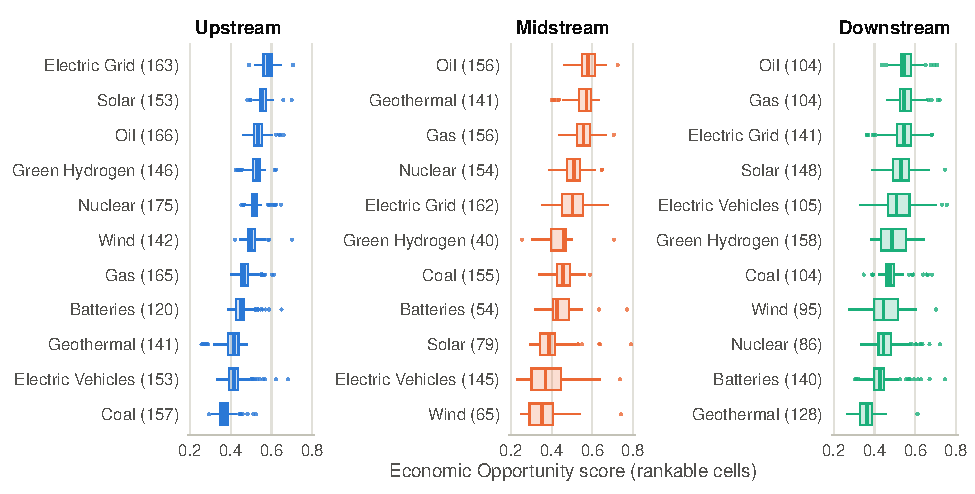
\includegraphics[width=\textwidth]{eo_distribution}
  \caption{Economic Opportunity by technology and stage over the rankable economies of each pair
  (number in parentheses, 40 to 175; sovereign economy with at most half of the index weight
  imputed). Boxes show the median and interquartile range, whiskers 1.5 interquartile ranges.
  Sample: 4{,}301 rankable of 7{,}131 scored cells; all 33 pairs have status \emph{ok}. Source:
  \texttt{economic\_opportunity\_index} in \texttt{index\_outputs.rds};
  \texttt{scripts/paper/fig\_eo.R}.}
  \label{fig:eo_distribution}
\end{figure}

\begin{figure}[tbp]
  \centering
  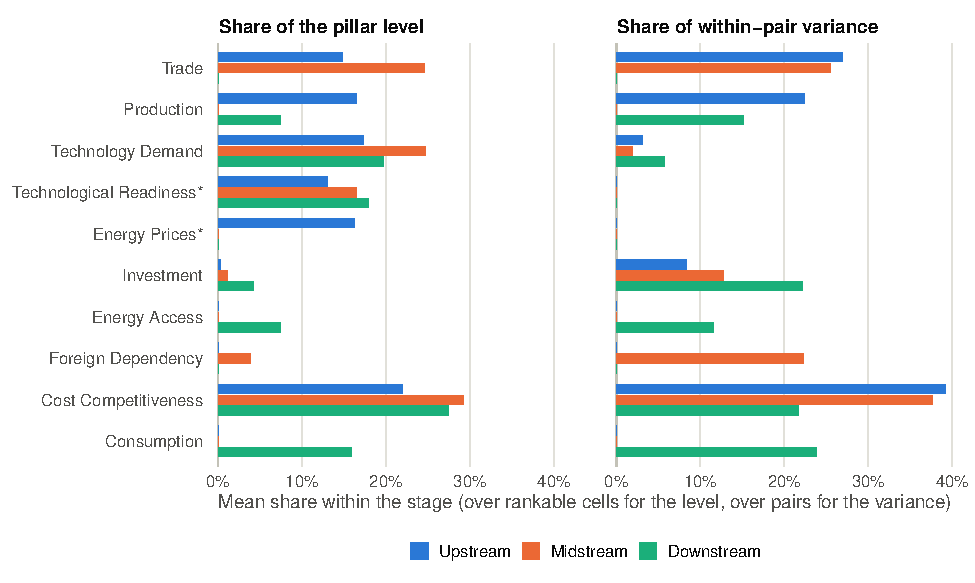
\includegraphics[width=\textwidth]{eo_contrib}
  \caption{Composition of Economic Opportunity by stage. Left: mean share of each category in the
  level, $\omega_{kits}c_{kits}/\EO_{its}$ (equation~\eqref{eq:cat_decomp}). Right: mean share in
  the within-pair variance, $\mathrm{cov}(\omega_{kits}c_{kits},\EO_{its})/\mathrm{var}(\EO_{its})$.
  Starred categories (Technological Readiness, Energy Prices) are constant within every pair;
  Technology Demand is constant except for its BNEF regional and EV-market composites. Sample:
  4{,}301 rankable cells. Source: category contributions in \texttt{index\_outputs.rds};
  \texttt{scripts/paper/fig\_eo.R}.}
  \label{fig:eo_contrib}
\end{figure}

\begin{figure}[tbp]
  \centering
  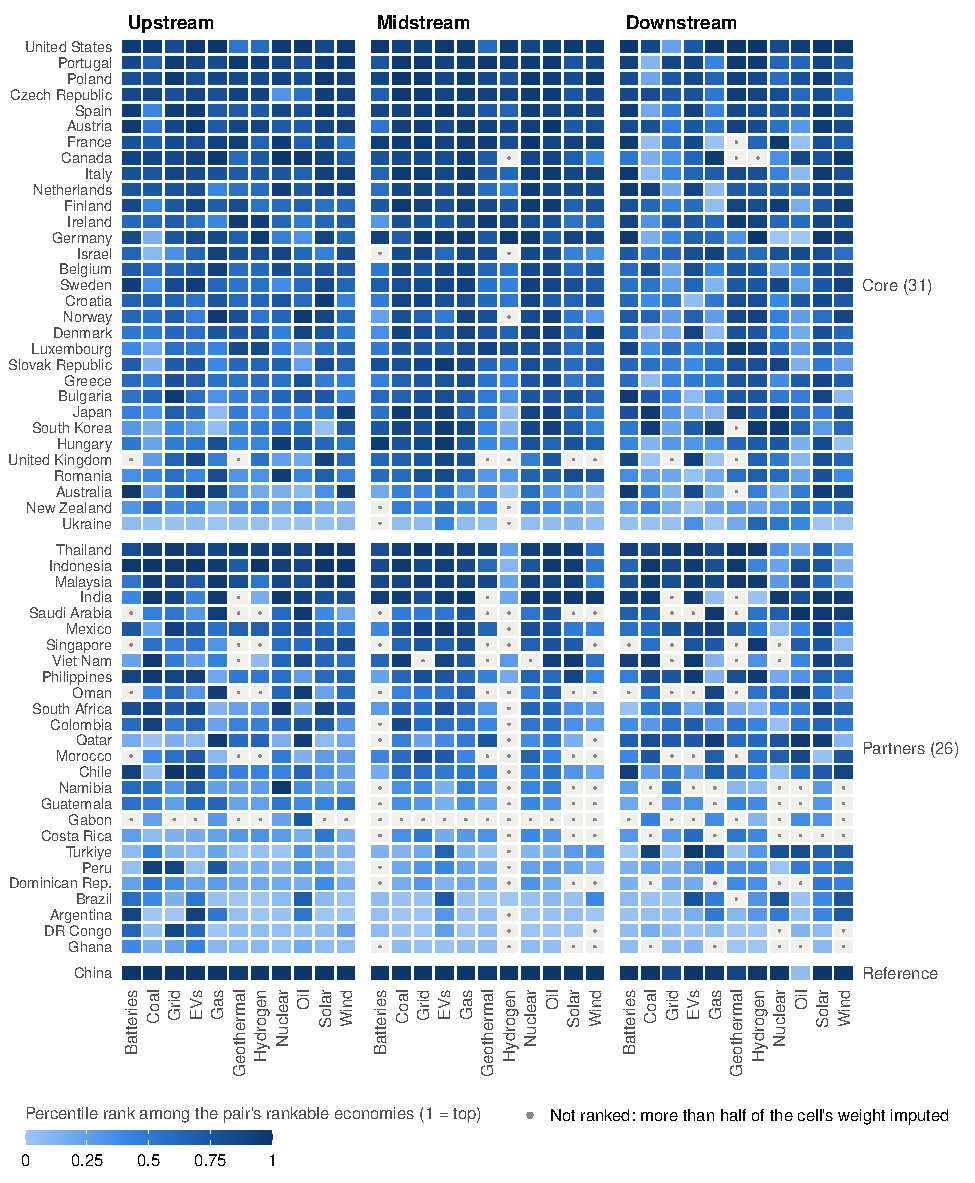
\includegraphics[width=\textwidth]{eo_heatmap}
  \caption{Within-pair percentile rank of $\EO_{its}$ (equation~\eqref{eq:pct_rank}) of the 31
  core members, the 26 partners (Section~\ref{sec:coalition}) and China, by pair. Ranks rather than
  levels are shown because pair effects account for 58 per cent of the variance of the level. Gray
  cells with a dot are scored but not rankable (more than half of the weight imputed). Source:
  \texttt{economic\_opportunity\_index}, \texttt{coalition\_members}; \texttt{scripts/paper/fig\_eo.R}.}
  \label{fig:eo_heatmap}
\end{figure}

\begin{figure}[tbp]
  \centering
  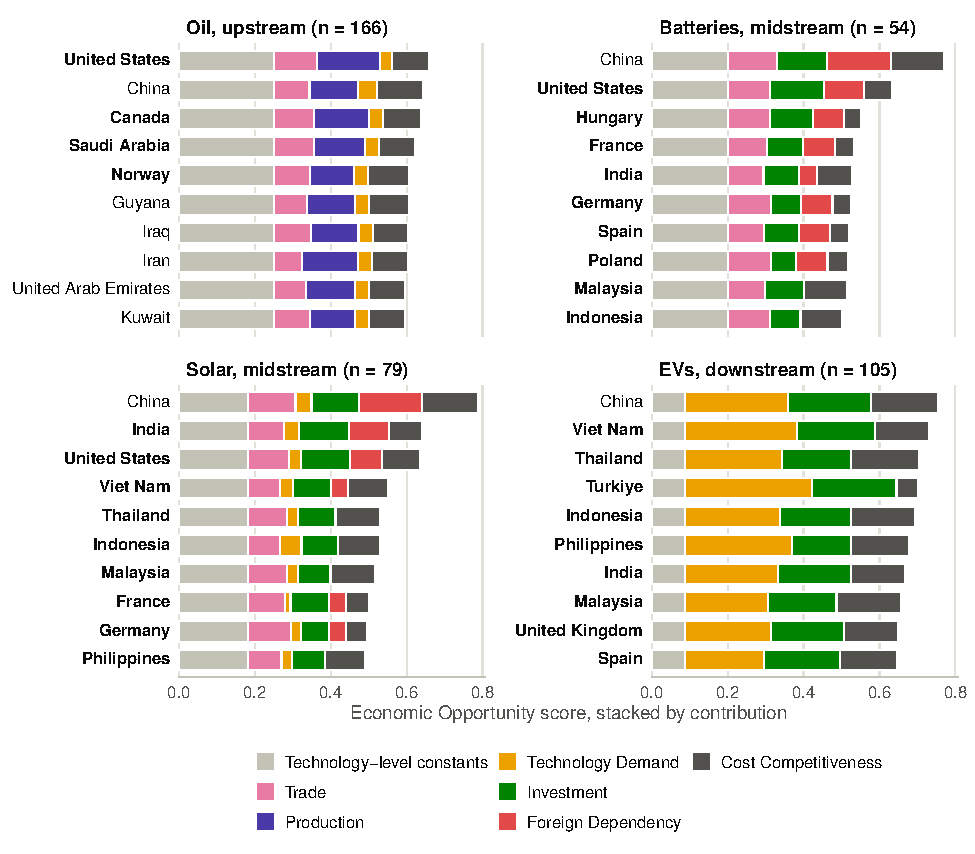
\includegraphics[width=\textwidth]{eo_top}
  \caption{The ten highest-scoring rankable economies in Oil upstream ($n=166$), Batteries
  midstream (54), Solar midstream (79) and EV downstream (105), stacked by the variable
  decomposition of equation~\eqref{eq:var_decomp}; colour identifies the category. The gray segment
  sums the technology-level constants (0.250, 0.202, 0.181 and 0.088), the same for every economy
  in a pair. Coalition members in bold. Source: \texttt{economic\_opportunity\_index} and its
  variable contributions; \texttt{scripts/paper/fig\_eo.R}.}
  \label{fig:eo_top}
\end{figure}

\FloatBarrier

% =============================================================================
% Section 7. The opportunity-security space
% Inputs: energy_security_index, economic_opportunity_index and their category and variable
% contributions (scripts/20_build_indices.R); the Strategic Index of Section 8 (eq:si).
% Results: paper/results/joint.json, scripts/paper/fig_joint.R (final rerun of 2026-10-12).
% Postures: RMI (2025) as labelled in config/country_insights.yml (quadrants) and
% R/charts/Country_Sector_Megatable.R (derive_strategic_path). Further results: Online Appendix
% (sections/oa_joint.tex, oa:joint).
% =============================================================================
\section{The opportunity-security space}\label{sec:joint}\label{sec:joint_space}

Each country-technology-stage cell is a point $(\ES_{its},\EO_{its})$ of the unit square. The
Strategic Index of Section~\ref{sec:strategic} reads the two pillars together, and its pillar terms
in equation~\eqref{eq:si} carry equal weights of opposite sign, so they reduce to the gap between
opportunity and security:
\begin{equation}\label{eq:joint_gap}
  0.3\,\EO_{its}+0.3\,(1-\ES_{its})=0.3+0.3\,\Delta_{its},\qquad
  \Delta_{its}\equiv\EO_{its}-\ES_{its}.
\end{equation}
The index favours cells in which opportunity exceeds security, and treats alike a cell that is
secure and well placed and one that is neither. Because it ranks a country's own sectors, what
matters is how $\Delta_{its}$ varies across them:
\begin{equation}\label{eq:joint_var}
  \operatorname{Var}_i(\Delta)=\operatorname{Var}_i(\EO)+\operatorname{Var}_i(\ES)
  -2\operatorname{Cov}_i(\EO,\ES).
\end{equation}
If the pillars rise together across a country's sectors, the gap is compressed and the policy term
and sector priors move the ranking more than their nominal weights suggest
\citep{paruolo2013ratings,becker2017weights}.

Part of the association is built in. Four categories enter both pillars with identical values, and
Trade and Foreign Dependency share components (Table~\ref{tab:shared_signals}). By the variable
decomposition of equation~\eqref{eq:var_decomp}, each pillar splits into the contribution of the
shared components and of the rest, $P_{its}=A^{P}_{its}+B^{P}_{its}$, and for any set of cells
\begin{equation}\label{eq:joint_cov}
  \operatorname{Cov}(\ES,\EO)=\operatorname{Cov}(A^{\ES},A^{\EO})
  +\operatorname{Cov}(A^{\ES},B^{\EO})+\operatorname{Cov}(B^{\ES},A^{\EO})
  +\operatorname{Cov}(B^{\ES},B^{\EO}).
\end{equation}
With fixed weights the first term is a positively weighted sum of the covariances of the shared
components: it records construction, not an economic link. In the gap those components enter with
coefficients $\omega^{\EO}\lambda^{\EO}-\omega^{\ES}\lambda^{\ES}$ and partly cancel
(equation~\eqref{eq:eo_si_shared}), so the information on where the gap is large lies mainly in
$B^{\ES}$ and $B^{\EO}$.

We report within-pair rank correlations from the full pillars and from $B^{\ES}$ and $B^{\EO}$
alone, and classify cells by each pillar's position relative to its within-pair median. The four
regions correspond to the four strategic postures of \citet{carey2025secure}, which read the same
two-dimensional space, in the labelling of the dashboard built on these indices: opportunity without security
(leapfrog: build capability), leaders (export promotion), laggards (friendshore: secure supply
through partners, the case of Sections~\ref{sec:bilateral} and~\ref{sec:network}) and security
without opportunity (alternative value creation). The correspondence is a reading aid, with the
median of each pair as the cut. As \citet{neis2026allied} stresses, security risk and economic
opportunity are not synonyms, and the same exposure can warrant different postures; the results
below measure how far the two pillars carry distinct information.

\subsection{Results}\label{subsec:joint_results}

\paragraph{Sample and co-movement.} Both pillars score 6{,}232 cells; 3{,}157 cells for 175
economies in 30 pairs are rankable on both (607 territory cells and 2{,}468 sovereign cells over
the imputation threshold are set aside), among them 1{,}500 cells of the 57 coalition members. The
median within-pair Spearman correlation of $\ES_{its}$ and $\EO_{its}$ is 0.59 (interquartile range
0.45 to 0.77), from $-0.21$ in Green Hydrogen midstream to 0.94 in Electric Vehicles midstream
(Table~\ref{tab:joint_stage}). It rises along the chain: 0.44 upstream, 0.58 midstream and 0.78
downstream (Figure~\ref{fig:joint_scatter}), a gradient that also holds within most technologies.

\begin{figure}[tbp]
  \centering
  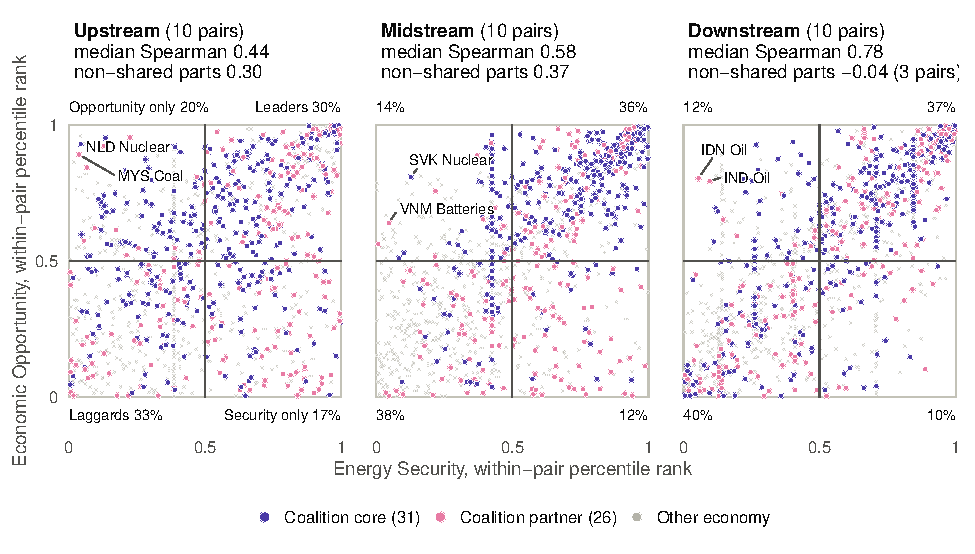
\includegraphics[width=\textwidth]{joint_scatter}
  \caption{The opportunity-security space. Each point is a cell rankable on both pillars, at its
  within-pair percentile rank on $\ES_{its}$ (horizontal) and $\EO_{its}$ (vertical); panels are
  stages. Violet: the 31 core members; pink: the 26 partners; gray: other economies. Lines at 0.5
  mark the within-pair medians and divide the regions (a cell at the median counts as low); corner
  percentages are the stage's shares. Panel headers give the median within-pair Spearman
  correlation from the full pillars and from the non-shared parts $B^{\ES}$, $B^{\EO}$ of
  equation~\eqref{eq:joint_cov}. The dense column left of the upstream security median is Nuclear
  upstream, where 87 of 175 economies without uranium share $\ES_{its}=0.172$. Sample: 3{,}157 cells,
  175 economies, 30 pairs. Source: \texttt{index\_outputs.rds}; \texttt{scripts/paper/fig\_joint.R}.}
  \label{fig:joint_scatter}
\end{figure}

\paragraph{How much is mechanical.} Shared components carry 61 per cent of the effective weight of
$\ES_{its}$ (25, 62 and 91 per cent by stage) but 28 per cent of that of $\EO_{its}$; in seven
downstream pairs every security component also enters opportunity. On the 23 pairs where both
pillars keep components of their own, the median correlation falls from 0.55 to 0.30 when only
non-shared components are used. The shared term accounts for 61 per cent of the pooled within-pair
covariance (7, 42 and 87 per cent by stage). What remains runs mainly through trade: the
largest cross-pillar category correlation is between security's Minerals Trade and opportunity's
Trade (0.76), while Technology Demand and Cost Competitiveness are nearly orthogonal to every
security category (Figure~\ref{fig:joint_corr}). Net of shared inputs, security and opportunity
are close to unrelated across economies except where exports reveal both.

% Generated by scripts/paper/fig_joint.R; do not edit by hand.
\begin{table}[tbp]
\centering
\begin{threeparttable}
\caption{Energy Security and Economic Opportunity within technology-stage pairs, by stage}
\label{tab:joint_stage}
\footnotesize
\begin{tabular}{@{}lcccc@{}}
\toprule
 & Upstream & Midstream & Downstream & All \\
\midrule
Technology-stage pairs & 10 & 10 & 10 & 30 \\
Country cells & 999 & 1,048 & 1,110 & 3,157 \\
\addlinespace
\multicolumn{5}{@{}l}{\textit{Spearman correlation of $\ES_{its}$ and $\EO_{its}$ within pairs}}\\
\quad Median across pairs & 0.44 & 0.58 & 0.78 & 0.59 \\
\quad Lowest pair & 0.03 & $-$0.21 & 0.40 & $-$0.21 \\
\quad Highest pair & 0.63 & 0.94 & 0.92 & 0.94 \\
\quad Pooled within-pair ranks & 0.39 & 0.60 & 0.71 & 0.57 \\
\addlinespace
\multicolumn{5}{@{}l}{\textit{Components shared by the two pillars}}\\
\quad Effective weight in $\ES$ & 0.25 & 0.62 & 0.91 & 0.61 \\
\quad Effective weight in $\EO$ & 0.26 & 0.20 & 0.37 & 0.28 \\
\quad Pairs with both non-shared pillars defined & 10 & 10 & 3 & 23 \\
\quad Median correlation, non-shared pillars & 0.30 & 0.37 & $-$0.04 & 0.30 \\
\quad Median correlation, full pillars, same pairs & 0.44 & 0.58 & 0.58 & 0.55 \\
\quad Share of level covariance, shared term & 0.07 & 0.42 & 0.87 & 0.61 \\
\quad Share of level covariance, non-shared term & 0.58 & 0.20 & 0.00 & 0.16 \\
\addlinespace
\multicolumn{5}{@{}l}{\textit{Share of cells by region of the space (percent)}}\\
\quad Opportunity without security & 19.5 & 13.8 & 12.4 & 15.1 \\
\quad Leaders (both high) & 30.2 & 36.0 & 37.2 & 34.6 \\
\quad Security without opportunity & 17.2 & 12.5 & 10.2 & 13.2 \\
\quad Laggards (both low) & 33.0 & 37.7 & 40.2 & 37.1 \\
\bottomrule
\end{tabular}
\begin{tablenotes}[flushleft]\footnotesize
\item \textit{Notes:} Eleven headline technologies; cells rankable on both pillars only (a sovereign economy with at most half of the pillar's weight imputed), which leaves 3,157 of the 6,232 cells that both pillars score, for 175 economies. A technology-stage pair enters when both pillars score it and neither pillar's diagnostics flag it as constant or unscored, which leaves 30 of the 33 pairs: Energy Security does not score downstream grid or upstream and midstream geothermal. Correlations are Spearman correlations across economies within a pair; the pooled row is the Pearson correlation of within-pair percentile ranks over all cells of the stage. A component is shared when the other pillar contains a component of the same category with identical observed values; its effective weight is its category weight times its within-category weight, averaged over cells. Non-shared pillars are the weighted means of the remaining components with the weights renormalised; they are undefined where every component of $\ES$ is shared, as in 7 downstream pairs, and the last two correlation rows use only the pairs in which both are defined. The covariance shares decompose the within-pair covariance of the pillar levels as in equation~\eqref{eq:joint_cov}, pooled over pairs with weights $n-1$: the shared term is $\operatorname{Cov}(A^{\ES},A^{\EO})$, the non-shared term $\operatorname{Cov}(B^{\ES},B^{\EO})$, and the two cross terms make up the remainder. Regions are defined by the within-pair medians of the two pillars, a cell at the median counting as low. Source: \texttt{index\_outputs.rds}; \texttt{scripts/paper/fig\_joint.R}.
\end{tablenotes}
\end{threeparttable}
\end{table}


\begin{figure}[tbp]
  \centering
  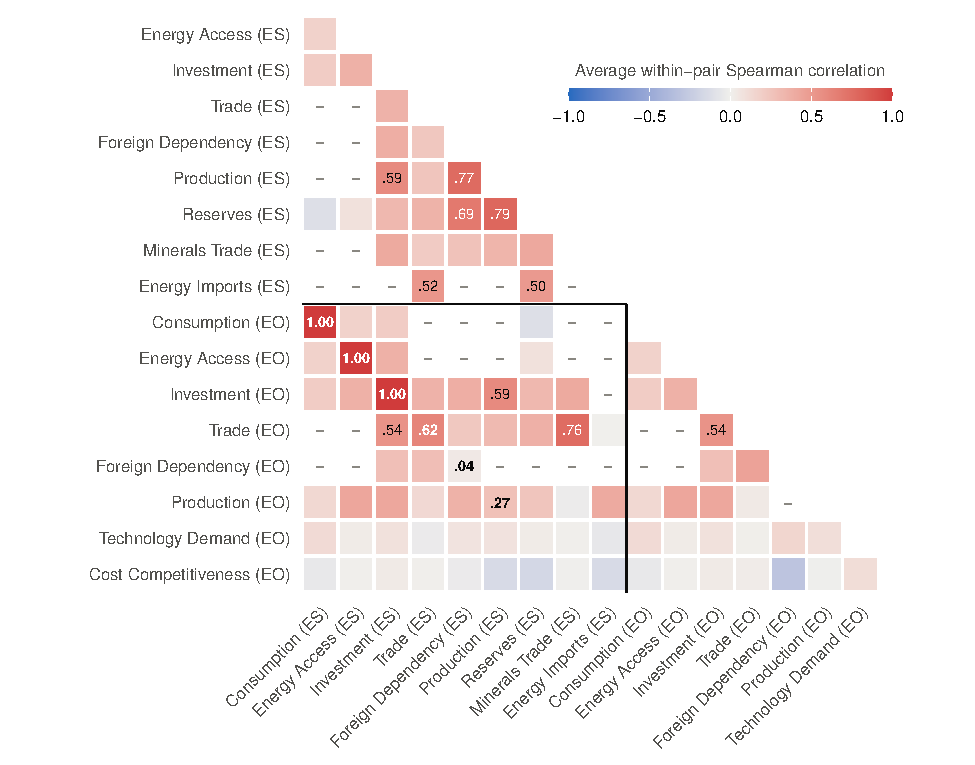
\includegraphics[width=\textwidth]{joint_corr}
  \caption{Average within-pair Spearman correlation between the categories of the two pillars
  (pairs with at least 20 rankable economies in which both categories vary). The black lines
  separate the cross-pillar block (bottom left) from the within-pillar blocks; bold numbers mark
  categories entering both pillars under the same name. Energy Prices and Technological Readiness,
  constant within every pair, are omitted. Sample: as Figure~\ref{fig:joint_scatter}. Source:
  category scores in \texttt{index\_outputs.rds}; \texttt{scripts/paper/fig\_joint.R}.}
  \label{fig:joint_corr}
\end{figure}

\paragraph{Regions.} Pooling all pairs, 15.1 per cent of cells have opportunity without security,
34.6 per cent are leaders, 13.2 per cent have security without opportunity and 37.1 per cent are
laggards (12.6, 37.7, 15.3 and 34.4 per cent if ties count as high). The shares largely restate the
rank correlation: a Gaussian copula with each pair's correlation implies an off-diagonal share of
14.6 per cent, against 14.2 observed. Opportunity without security is most common upstream (19.5
per cent), where the pillars are least related. The largest pair shares, Green Hydrogen midstream
(45 per cent) and Nuclear upstream (28), are tie artefacts (Figure~\ref{fig:joint_quadrants});
without them the pooled share is 14.0 per cent.

\begin{figure}[tbp]
  \centering
  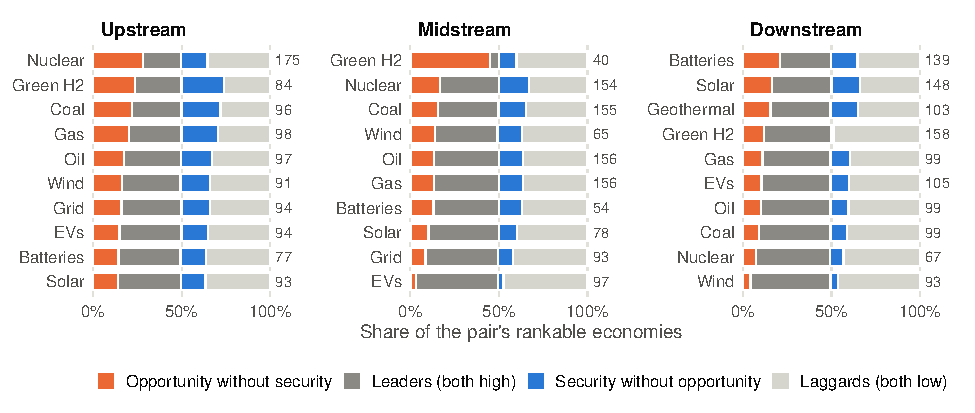
\includegraphics[width=\textwidth]{joint_quadrants}
  \caption{Shares of each pair's rankable economies in the four regions of
  Figure~\ref{fig:joint_scatter}, by stage, ordered by the share with opportunity but not security
  (orange); blue marks security without opportunity, dark gray leaders, light gray laggards. The
  two longest orange segments are ties at the security median: in Green Hydrogen midstream 34 of
  40 economies share the lowest $\ES_{its}$, and in Nuclear upstream 87 of 175 share the median
  value. Source: as Figure~\ref{fig:joint_scatter}.}
  \label{fig:joint_quadrants}
\end{figure}

\paragraph{The coalition.} Of the members' cells, 49.3 per cent are leaders and 12.8 per cent have
opportunity without security (core 55.1 and 16.4 per cent, partners 40.4 and 7.4;
Figure~\ref{fig:joint_members}), partly because scale raises both pillars; the United States is a
leader in 29 of 30 pairs. Austria, Portugal and Luxembourg have the most leapfrog-type pairs (11 of
30 each); Brazil (19 of 29), Peru and T\"urkiye have the most security without opportunity.

\begin{figure}[tbp]
  \centering
  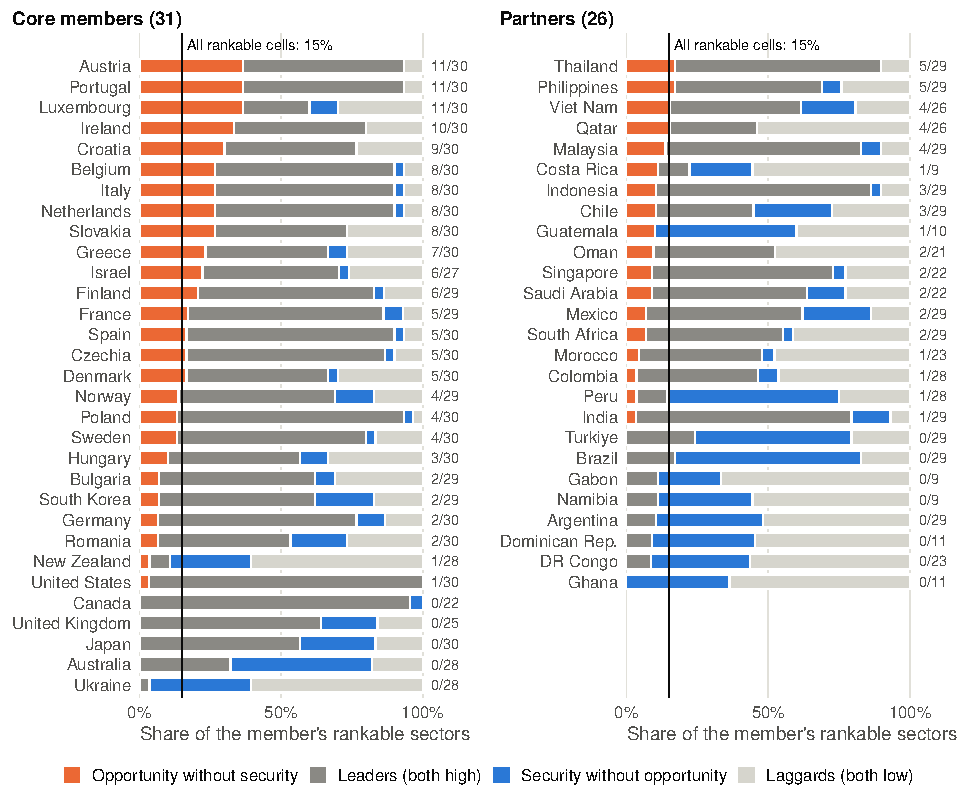
\includegraphics[width=\textwidth]{joint_members}
  \caption{Each coalition member's rankable pairs divided among the four regions: the 31 core
  members (left) and 26 partners (right), ordered by the share with opportunity but not security;
  the fraction gives that count over the member's rankable pairs (9 to 30). The vertical line is
  the all-cell share (15 per cent). Nuclear upstream and Green Hydrogen midstream account for 25 of
  the 192 member pairs in orange. Source: as Figure~\ref{fig:joint_scatter}.}
  \label{fig:joint_members}
\end{figure}

\paragraph{Within countries and the Strategic Index.} Across the sectors of each of the 167
countries with at least five Strategic Index cells, the correlation of $\EO_{its}$ and $\ES_{its}$
averages 0.46 (from $-0.56$ to 0.84), and the covariance term removes on average 36 per cent of
$\operatorname{Var}_i(\EO)+\operatorname{Var}_i(\ES)$ (42 per cent for members), leaving a standard
deviation of $\Delta_{its}$ of 0.13. The index does favour the leapfrog region (mean 0.563 there,
against 0.511 to 0.545 elsewhere), and 8 of the 57 allied picks lie in it (14.0 per cent, against
6.7 per cent of eligible sectors). Four of the nine Nuclear midstream picks come from small
partners with four or five eligible sectors; their security ranks lie at or above a compressed
median, so the picks reflect the technology weight of equation~\eqref{eq:si} (0.999 for nuclear
against 0.42 for gas), not a security floor. Across a country's sectors the index correlates 0.63
with the level gap but only 0.19 with the gap in within-pair ranks: it reflects which pairs score
high opportunity and low security for everyone at least as much as where the country stands.
Online Appendix~\ref{oa:joint} gives further detail and caveats.

% Section 7.5: Geopolitical alignment and the allied coalition.
% Specification: R/geopolitical_distance/{ideal_points,alignment}.R and scripts/12 (ideal points,
% blocs, dyadic alignment); R/indices/coalition.R and scripts/13 (tiers, routes, EU node weights);
% config/coalition.yml, config/geopolitical_distance.yml. Numbers: paper/results/coalition.json
% (final rerun of 2026-10-12); figures and table: scripts/paper/fig_coalition.R.
\section{Geopolitical alignment and the allied coalition}\label{sec:coalition}

Three parts of the analysis need a coalition: the allied picks of the Strategic Index
(Section~\ref{sec:strategic}), the viewpoint from which the Partnership Strength Index rates partners
(Section~\ref{sec:bilateral}) and the nodes of the network design (Section~\ref{sec:network}). We
derive it by rule from two observable attributes, an economy's alignment in the United Nations
General Assembly and its weight in world supply, rather than fixing it by hand.

\subsection{Ideal points and the U.S.--China axis}\label{subsec:coalition_axis}

Alignment is measured with the ideal points of \citet{bailey2017estimating}, which place every
voting state on one dimension of revealed foreign-policy preference, bridged so that positions are
comparable across sessions. We use the all-votes series of the July 2026 release
\citep[Dataverse V39;][]{voeten2009unga} and average each economy's ideal point $\theta_i$ over
sessions 74 to 78 (2019--2023), which covers the 193 economies that vote in their own right. Each is
placed on the segment between the two anchors,
\begin{equation}\label{eq:coalition_axis}
  s_i \;=\; \min\Bigl\{1,\;\max\Bigl\{0,\;
  \frac{\theta_i-\theta_{\mathrm{CHN}}}{\theta_{\mathrm{USA}}-\theta_{\mathrm{CHN}}}\Bigr\}\Bigr\},
\end{equation}
so that $s_i=0$ is China's position and $s_i=1$ that of the United States
($\theta_{\mathrm{USA}}=2.34$, $\theta_{\mathrm{CHN}}=-1.02$). Seven economies vote further from the
United States than China does and are clamped to zero (Cuba, Iran, Nicaragua, North Korea, Syria,
Venezuela and Zimbabwe). The axis records revealed preferences relative to two anchors, not alliance
or any bilateral relationship.

Following \citet{gopinath2025changing}, blocs are quartiles of the axis: the U.S.-leaning bloc is
the quarter of voting economies closest to the United States ($s_i\geq 0.511$, 49 economies), the
China-leaning bloc the quarter closest to China ($s_i\leq 0.142$, 49), and the 95 in between are
nonaligned. Membership is hard: the bloc indicator $p_i$ is 1 for U.S.-leaning, $\tfrac12$
for nonaligned and 0 for China-leaning economies. Because the United States often votes in small minorities, the distribution is
skewed toward China (median $s=0.22$), and a midpoint rule would call 142 of 193 economies
China-leaning; quartiles keep that bloc to the quarter of the Assembly closest to China. After the
cuts are set, 44 territories inherit their sovereign's bloc and Taiwan, Palestine and Kosovo are
neutral ($p_i=\tfrac12$); these assignments serve only the bilateral indices, and an economy
without its own vote cannot be a core member.

For a pair of economies the dyadic alignment is
\begin{equation}\label{eq:coalition_dyadic}
  A_{ij} \;=\; p_i\,p_j + (1-p_i)(1-p_j),
\end{equation}
which would be the probability that $i$ and $j$ fall on the same side of the divide if $p_i$ were
a probability; with hard blocs it is 1 for the same bloc, 0 for opposite blocs and $\tfrac12$ whenever either is nonaligned. It is a Friendshore
component with weight 2 of 11 (Section~\ref{subsec:friendshore}) and through Friendshore enters the
edge term of the network design. Figure~\ref{fig:coalition_axis} shows the axis by coalition tier.

\begin{figure}[tbp]
  \centering
  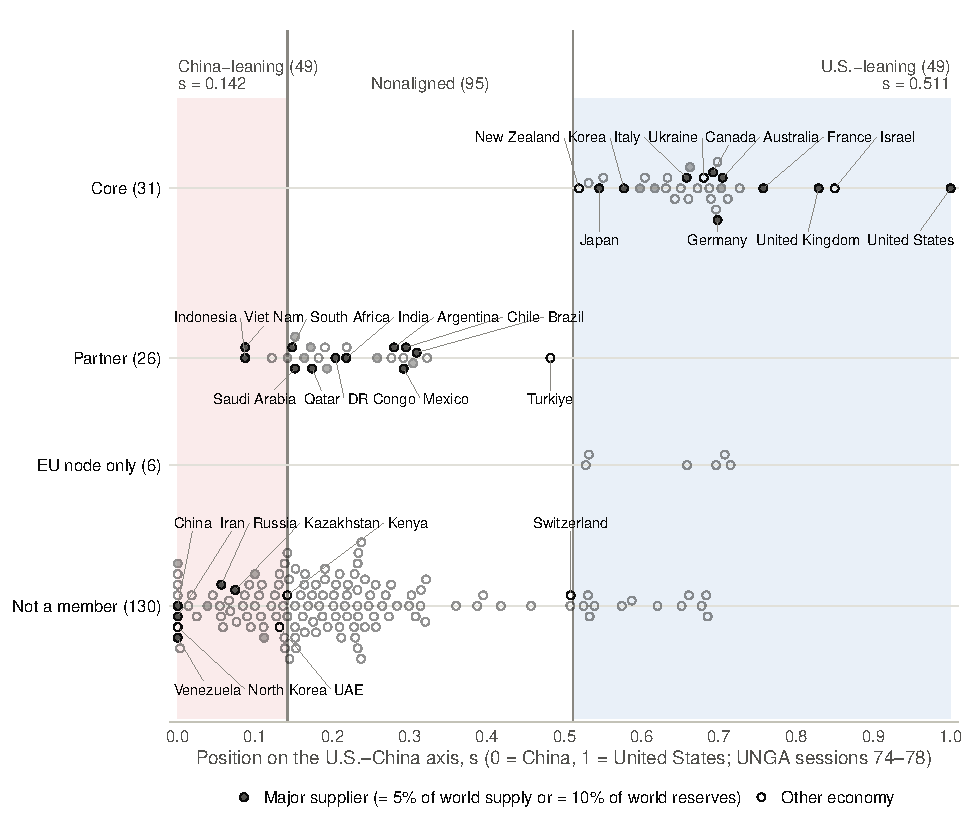
\includegraphics[width=\textwidth]{coalition_axis}
  \caption{Positions on the U.S.--China axis and coalition tiers. Each point is one of the 193
  economies with their own votes in the General Assembly, at $s_i$ of
  equation~\eqref{eq:coalition_axis}: the mean all-votes ideal point of
  \citet{bailey2017estimating} over sessions 74--78 (2019--2023), projected on the segment from China
  ($s=0$) to the United States ($s=1$) and clamped to $[0,1]$. Vertical lines are the quartile cuts
  ($s\leq 0.142$ China-leaning, $s\geq 0.511$ U.S.-leaning; 49, 95 and 49 economies). Rows are the 31
  core members, the 26 partners, the six EU members that enter only through the EU node and the 130
  other voting economies; vertical position within a row carries no information. Filled markers are
  major suppliers (at least 5 percent of world supply in an Upstream or Midstream stage, or at least
  10 percent of world reserves of a headline mineral, fuel or uranium). G20 economies and selected
  other cases are labelled. Source: \texttt{geo\_ideal\_points\_tbl.rds}, \texttt{coalition\_tbl.rds},
  \texttt{major\_supplier\_shares\_tbl.rds}.}
  \label{fig:coalition_axis}
\end{figure}

\subsection{A coalition in two tiers}\label{subsec:coalition_tiers}

The \emph{core} of the coalition $\Coalition$ is the U.S.-leaning bloc restricted to economies with
their own UN votes and a GDP of at least USD 100 billion \citep[2025;][]{worldbank2026wdi}: 31
economies. An economy outside the core is a \emph{partner} if it qualifies by either of two routes.
The agreement route admits members of a U.S. free trade agreement, the Indo-Pacific Economic
Framework (IPEF), the Minerals Security Partnership (MSP), the G7 or NATO with GDP of at least USD
100 billion, whatever their bloc. The supplier route admits, without a GDP floor, any economy that is
not China-leaning and is a major supplier of an Upstream or Midstream stage of a headline
technology: it holds at least 5 percent of world supply in one measure of the stage (exports of the
stage's HS6 basket, fuel or uranium production, mineral mining or refining, or manufacturing
capacity), or at least 10 percent of world reserves of a resource the stage extracts, read from
the reserves tables of the Energy Security pillar \citep{usgs2026mcs,ei2026statistical,oecdnea2026uranium}.
The reserves bar is twice the supply bar because a stock is not yet supply; holders that USGS does
not quantify count as zero. Online Appendix~\ref{oa:coalition} lists the source and year of each
measure.

The rule yields 26 partners (Table~\ref{tab:coalition_composition},
Figure~\ref{fig:coalition_routes}): ten qualify through agreements only, nine as suppliers only and
seven by both routes. Twenty-three are nonaligned and three China-leaning: Indonesia and Viet Nam,
members of IPEF, and Oman, a U.S. free-trade partner. The 57 members account for 73.4 percent of
world GDP (core 57.7, partners 15.7); China accounts for 16.6 percent.

Forty economies pass the supplier test, and every one that is not China-leaning is a member. The
nine China-leaning major suppliers are kept out: China, Russia, Iran, Kazakhstan, Algeria,
Uzbekistan, Venezuela, Myanmar and Zimbabwe, with largest qualifying shares from 94.4 percent of
world graphite refining (China) and 45.1 percent of exports of the uranium basket (Kazakhstan) to 5.1
percent of gas exports (Algeria). Eleven members hold at least 10 percent of a world reserve (Indonesia,
China-leaning, cannot use the supplier route), and for none of the other ten is the reserves leg
decisive. Brazil, in none of the five agreements, holds 23.9 percent of
world graphite reserves, 16.7 percent of manganese, 14.6 percent of rare earths and 11.4 percent of
nickel, and also supplies 18.4 percent of world exports of silicon metal (the Solar Upstream basket).
Among all economies the reserves leg is decisive only for Venezuela, which is kept out.

% Generated by scripts/paper/fig_coalition.R from data/processed/coalition_tbl.rds,
% geo_ideal_points_tbl.rds and major_supplier_shares_tbl.rds
\begin{table}[htbp]
\centering
\begin{threeparttable}
\caption{Composition of the allied coalition}
\label{tab:coalition_composition}
\footnotesize
\begin{tabularx}{\textwidth}{@{}>{\raggedright\arraybackslash}p{0.27\textwidth} r >{\raggedright\arraybackslash}X@{}}
\toprule
Group & $n$ & Economies \\
\midrule
Core: U.S.-leaning bloc, GDP $\geq$ USD 100bn & 31 & United States, Germany, Japan, United Kingdom, France, Italy, Canada, Spain, Korea, Australia, Netherlands, Poland, Belgium, Ireland, Sweden, Israel, Austria, Norway, Denmark, Romania, Czechia, Portugal, Finland, Greece, New Zealand, Hungary, Ukraine, Slovakia, Bulgaria, Croatia, Luxembourg \\
Partners, agreement route only & 10 & T\"urkiye (NATO), Indonesia (IPEF), Singapore (IPEF, U.S. FTA), Thailand (IPEF), Viet Nam (IPEF), Morocco (U.S. FTA), Dominican Rep. (U.S. FTA), Guatemala (U.S. FTA), Oman (U.S. FTA), Costa Rica (U.S. FTA) \\
Partners, supplier route only & 9 & Brazil (Solar Up 18\% [+3]), Saudi Arabia (Oil Up 13\%), Argentina (Batteries Up 6\% [+1]), South Africa (Hydrogen Up 52\% [+3]), Qatar (Gas Up 14\%), Ghana (Batteries Up 10\% [+2]), DR Congo (Batteries Up 66\% [+9]), Gabon (Batteries Up 25\% [+2]), Namibia (Nuclear Up 12\%) \\
Partners, both routes & 7 & India (IPEF, MSP), Mexico (U.S. FTA), Philippines (IPEF), Malaysia (IPEF), Colombia (U.S. FTA), Chile (U.S. FTA), Peru (U.S. FTA) \\
EU members in the EU node only & 6 & Lithuania, Slovenia, Latvia, Estonia, Cyprus, Malta \\
Major suppliers kept out (China-leaning) & 9 & China (Batteries Mid 94\% [+16]), Russia (Hydrogen Up 29\% [+6]), Iran (Gas Up 6\% [+1]), Kazakhstan (Nuclear Up 45\%), Algeria (Gas Up 5\%), Uzbekistan (Nuclear Up 8\%), Venezuela (Oil reserves 18\%), Myanmar (Wind Up 31\% [+1]), Zimbabwe (Batteries Up 9\% [+2]) \\
Reserves holders between 5\% and 10\%, not members & 6 & Madagascar (Graphite 8.7\%), Mozambique (Graphite 8.1\%), Kuwait (Oil 5.9\%), Tanzania (Graphite 5.8\%), Niger (Uranium 5.7\%), New Caledonia (Nickel 5.1\%) \\
Added by the MSP Forum sensitivity & 3 & Kazakhstan, Uzbekistan, Ecuador \\
Hand-picked list of the previous draft: not members & 2 & UAE, Kenya \\
Hand-picked list of the previous draft: members & 21 & 11 in the core, 10 partners \\
\bottomrule
\end{tabularx}
\begin{tablenotes}[flushleft]\footnotesize
\item \emph{Notes:} Economies are ordered by GDP within a group. Core: the U.S.-leaning quartile bloc of the all-votes ideal points of \citet{bailey2017estimating} over UNGA sessions 74--78 (2019--2023), $s\geq 0.511$, with the economy's own UN votes and latest World Bank GDP of at least USD 100bn. Partners (not core): a member of a U.S. free trade agreement, IPEF, the Minerals Security Partnership (MSP), the G7 or NATO with GDP of at least USD 100bn (qualifying agreements in parentheses), or, without a GDP floor, an economy that is not China-leaning and holds at least 5\% of world supply in one measure of an Upstream or Midstream stage of a headline technology (exports of the stage's HS6 basket, fuel or uranium production, mineral mining or refining, or manufacturing capacity) or at least 10\% of world reserves of a headline mineral, fuel or uranium. For the supplier route, the parentheses give the largest qualifying share: the technology--stage cell of a supply measure, or the resource when only reserves qualify, and in brackets the number of further qualifying cells. The six EU members below the GDP floor belong to the coalition only through the EU. The MSP Forum sensitivity admits Forum members by the agreement route. The previous draft's 23 members were fixed by hand.
\end{tablenotes}
\end{threeparttable}
\end{table}


\begin{figure}[tbp]
  \centering
  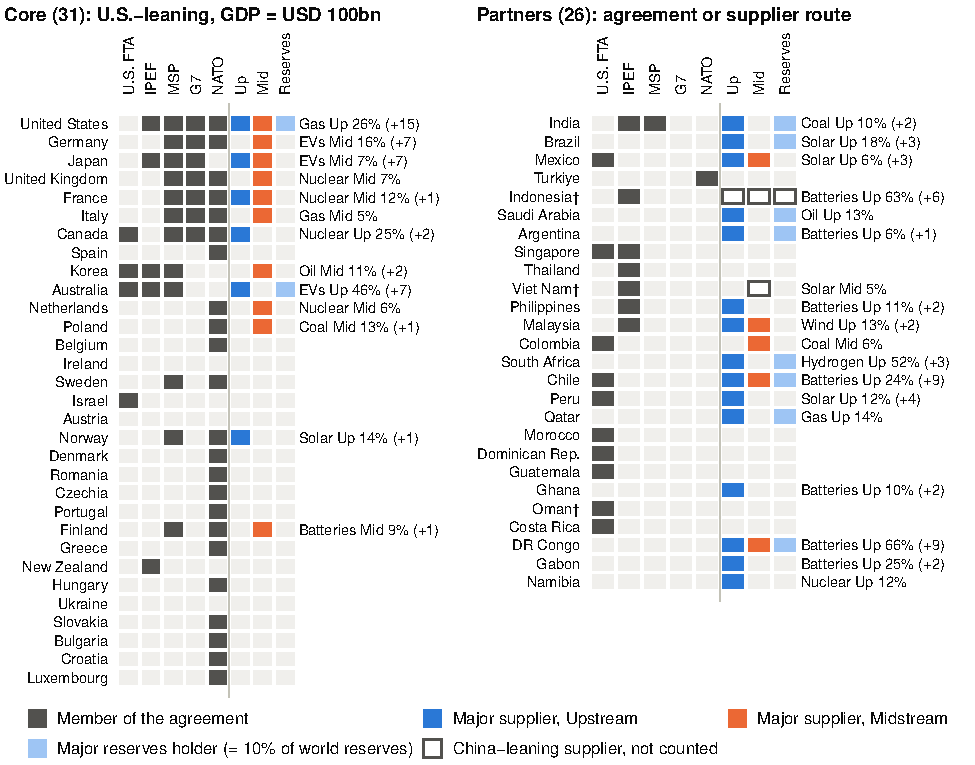
\includegraphics[width=\textwidth]{coalition_routes}
  \caption{Routes into the coalition. Rows are the 31 core members (left) and the 26 partners
  (right), ordered by GDP. Gray tiles mark membership of the five agreements of the agreement route
  (U.S. free trade agreement, IPEF, MSP, G7, NATO). Coloured tiles mark the supplier test: at least
  5 percent of world supply in an Upstream (blue) or Midstream (orange) stage, or at least 10 percent
  of world reserves (light blue). Outlined tiles ($\dagger$) mark economies that pass the test but are
  China-leaning and so cannot use the supplier route; Indonesia and Viet Nam enter through IPEF and
  Oman through its U.S. free trade agreement. The core requires neither route. The text gives the
  largest qualifying share, with the number of further qualifying cells in parentheses. Source:
  \texttt{coalition\_tbl.rds}, \texttt{major\_supplier\_shares\_tbl.rds},
  \texttt{economic\_security\_agreements.csv}.}
  \label{fig:coalition_routes}
\end{figure}

Two economies a reader might expect are not members. Switzerland is nonaligned at $s=0.508$, three
thousandths below the U.S.-leaning cut, belongs to none of the agreements, and its largest supply
share is 1.1 percent; its former supplier route rested on electricity exports, no longer part of
the Electric Grid basket (Section~\ref{sec:data}). Taiwan has no UN vote and is therefore neutral,
appears in no agreement list and has no World Bank GDP; its largest share is 1.5 percent (Solar
Midstream exports), and its semiconductor strength lies outside the energy baskets. Both remain
partners in the bilateral indices but are not network nodes.

The coalition is long in mining and short in processing: its economies mine 81.9 percent of the
world's cobalt and 60.0 percent of its lithium but refine 17.4 and 24.6 percent, and 5.5 percent of
graphite, against China's 75.6, 73.7 and 94.4 percent \citep{iea2026cmdata}; Online
Appendix~\ref{oa:coalition} gives the supply cover by stage.

\subsection{Network nodes and the European Union}\label{subsec:coalition_nodes}

The EU-27 enters the network design as a single node, because the Union conducts a common
commercial policy and its members' supply chains are integrated in a single market. Twenty-one EU
members are core members in their own right; the six below the GDP floor (Cyprus, Estonia, Latvia,
Lithuania, Malta and Slovenia, 1.6 percent of EU GDP) belong to the network only through the node.
The network therefore has 37 nodes representing 63 economies: 11 core nodes (the United States, the
EU, Japan, the United Kingdom, Canada, Korea, Australia, Israel, Norway, New Zealand and Ukraine) and
26 partner nodes. The node's demand enters the design through ranks and is therefore compressed
relative to the EU's share of coalition GDP (Section~\ref{sec:network}).

Members' inputs are aggregated into the node with stage-specific weights
(Figure~\ref{fig:coalition_eu_weights}): production for Coal, Gas and Oil Upstream, exports of the
stage's HS6 basket for 15 cells and GDP for the four Geothermal and Green Hydrogen cells, which have
no basket. The weights are concentrated: Germany carries the largest weight in 11 of the 22 cells,
and France 97.9 percent of the EU's uranium-basket exports although it mines no uranium, trade that
reflects conversion and trading rather than mine output.

\begin{figure}[tbp]
  \centering
  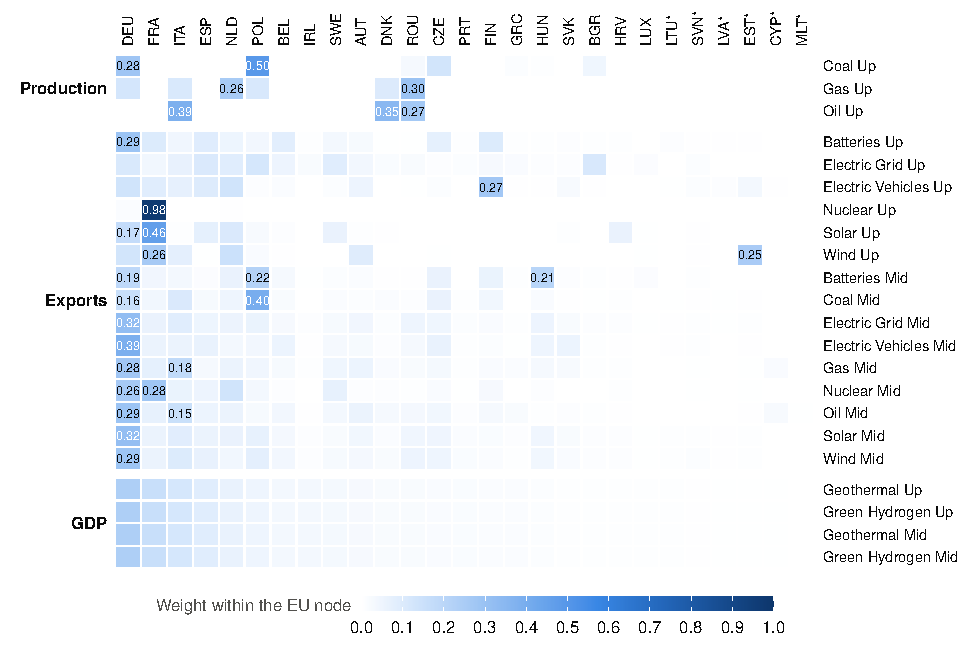
\includegraphics[width=\textwidth]{coalition_eu_weights}
  \caption{Member weights within the EU network node. Columns are the 27 EU members, ordered by GDP;
  an asterisk marks the six members below the GDP floor, which enter the network only through the
  node. Rows are the 22 Upstream and Midstream cells, grouped by the basis of the weights: members'
  production (Energy Institute; 3 cells), members' shares of world exports of the stage's HS6 basket
  (15 cells) or, for the four stages without a basket, GDP shares (Geothermal and Green Hydrogen,
  Upstream and Midstream). Weights in a row sum to one; weights of at least 0.15 under the production
  and export bases are printed. Median Herfindahl index of the weights: 0.34 (production), 0.139
  (exports), 0.117 (GDP). Source: \texttt{eu\_stage\_weights\_tbl.rds}.}
  \label{fig:coalition_eu_weights}
\end{figure}

\subsection{Alignment within the coalition}\label{subsec:coalition_dyadic}

Because the blocs are hard, alignment within the coalition takes a simple form
(Figure~\ref{fig:coalition_alignment_matrix}). Of the 666 pairs of network nodes, 8.7 percent have
$A_{ij}=1$ (pairs of core nodes and pairs among the three China-leaning partners), 86.3 percent have
$A_{ij}=\tfrac12$ because one of the two is a nonaligned partner, and 5.0 percent have $A_{ij}=0$:
each core node paired with Indonesia, Viet Nam or Oman. The alignment component of Friendshore thus
separates core from partner-tier members and penalises the three China-leaning partners as
friendshoring partners of the core, but leaves the ordering of the 23 nonaligned partners to the other components.

\begin{figure}[tbp]
  \centering
  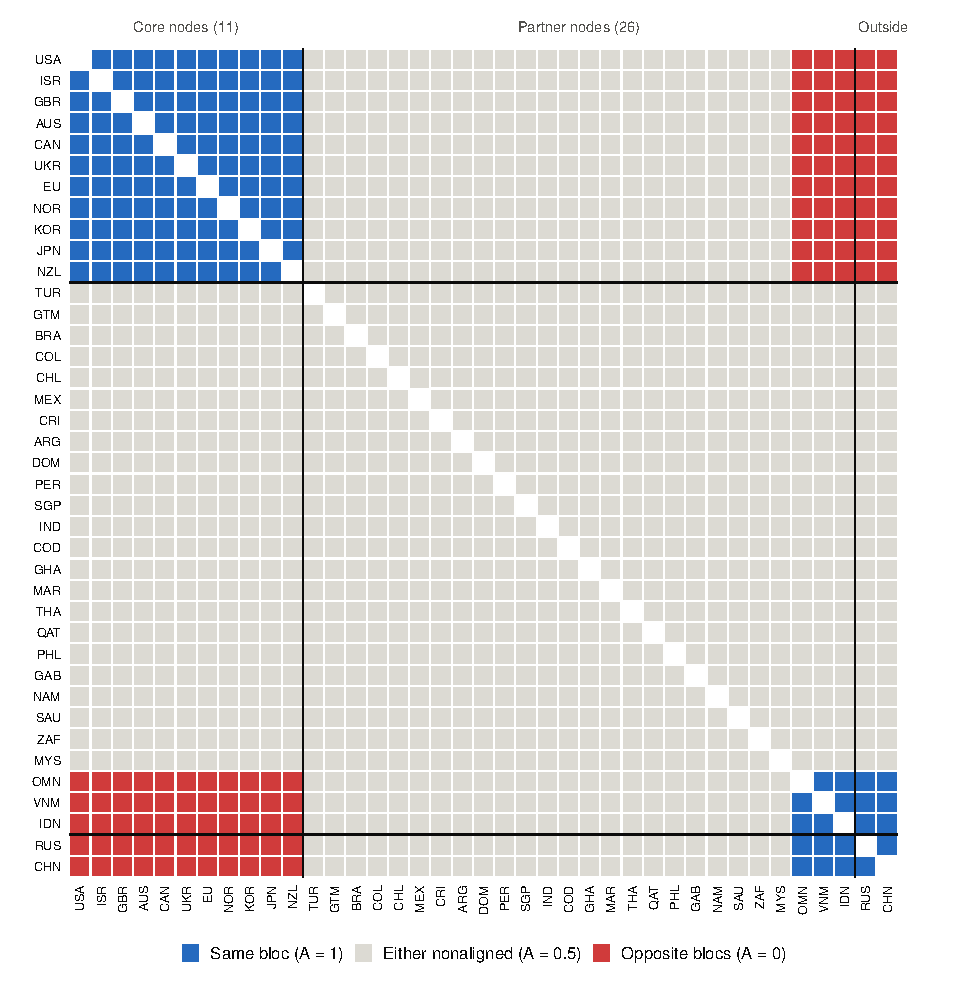
\includegraphics[width=\textwidth]{coalition_alignment_matrix}
  \caption{Dyadic alignment among the network nodes. Each cell is $A_{ij}$ of
  equation~\eqref{eq:coalition_dyadic}: 1 for the same bloc, 0 for opposite blocs and $\tfrac12$
  when either economy is nonaligned. The 37 network nodes, 11 core and 26 partner, are followed by
  Russia and China for reference, ordered by tier and, within a tier, by $s$ (for the EU node, the
  GDP-weighted mean of its members, 0.677; all 27 members are U.S.-leaning). Source:
  \texttt{geo\_alignment\_tbl.rds}, \texttt{allied\_network\_nodes.csv}.}
  \label{fig:coalition_alignment_matrix}
\end{figure}

\subsection{Sensitivity and comparison with the hand-picked list}\label{subsec:coalition_sensitivity}

Two alternative vote series test the axis. With session 78 alone the Spearman correlation of $s$
with the headline is 0.966, 89.1 percent of economies keep their bloc and the coalition keeps 57
members, with three changes at the margin. With the final-passage series over sessions 76--80
(2021--2025) the correlation is 0.965 and the core is unchanged, but the China-leaning cut falls to
0.055: Russia, Kazakhstan and Myanmar leave the China-leaning quartile and would enter as major
suppliers, for 60 members. The core is robust to the vote series; the exclusion of China-leaning
suppliers is the fragile element of the rule. Admitting the MSP Forum as a further agreement adds
Kazakhstan, Uzbekistan and Ecuador.

The derived coalition replaces a list of 23 economies fixed by hand in an earlier version
(Appendix~\ref{app:corrections}). Twenty-one remain; the United Arab Emirates and Kenya, both
China-leaning, in no agreement and without a qualifying share, leave; 36 economies join.

\paragraph{The rule and a functional definition of ``allied''.} The working paper on the Allied
Industrial Base \citep{neis2026allied} argues that ``allied'' should be a functional rather than a
treaty category, with partners assessed on reliability and contractual performance, economic
complementarity, strategic alignment, burden sharing, technology-security requirements and
contribution to system resilience, and with membership varying across sectoral compacts. The derived
coalition implements part of that programme: the axis measures strategic alignment, the supplier
route contribution to world supply and reserves, and the agreement route economic-security ties
with the United States that are already institutionalised. It does not measure reliability, the
rule of law, burden sharing or technology-security requirements, and it defines one coalition for
all 22 stages. The supplier route gives the boundary a sectoral margin (nine partners qualify only
as suppliers of particular stages), but a coalition defined stage by stage, admitting a resource
holder to a minerals compact without admitting it to one on sensitive grid equipment, is left to
future work.

% Section 8: The Policy index and the Strategic Index.
% Specification: R/categories/policy/{iea_policy_index,cat_policy_index}.R,
% R/indices/build_policy_index.R (build_composite_policy_index; POLICY_COMPONENT_WEIGHTS = IEA PAMS 3,
% CAT 2; IEA PAMS required), R/indices/build_indices.R (build_strategic_index,
% strategic_index_degenerate_sectors, strategic_index_es_floor_sectors, strategic_resource_base,
% flag_strategic_resource_base, select_allied_strategic_sectors), the policy block of
% scripts/10_build_themes.R and scripts/20_build_indices.R. Numbers: paper/results/strategic.json and
% si_fixed_inputs.json (final rerun of 2026-10-12); figures and table: scripts/paper/fig_strategic.R,
% fig_si_fixed_inputs.R. POL^*_{its} is the within-country S-curve of the Policy index (the code's pol).
% Further detail: sections/oa_strategic.tex (oa:strategic).
\section{The Policy index and the Strategic Index}\label{sec:strategic}

This section constructs a Policy index $\POL_{its}$ of recorded policy activity in each cell and a
Strategic Index $\SI_{its}$ that combines it with the two pillars and two fixed sector weights into
a ranking of each country's sectors, from which one allied pick is drawn for each coalition member.
Both have normative weights \citep{oecd2008handbook,decancq2013weights}; we state each and report
the choices to which the rankings are sensitive.

\subsection{The Policy index}\label{subsec:policy_composite}

No measure of industrial policy captures whether a policy is well designed
\citep{juhasz2024new,juhasz2022who,evenett2024return}. The Policy index measures the intensity and
direction of state attention to a cell, which indicates where capacity is likely to be built and
sustained \citep{rodrik2004industrial,rodrik2014green}, not whether that attention is warranted. It
has two components.

\paragraph{IEA Policies and Measures.}\label{subsec:policy_iea} The IEA database records national,
subnational and international energy and climate policies with their status, jurisdiction, type and
text \citep{iea2026pams}. Each policy $h$ is assigned to technologies and stages by keyword rules and
given a strength $\sigma_h$, the product of type, status and jurisdiction weights and of discounts
for cross-cutting or text-only assignments. The component is the S-curve of the log summed strength,
ranked over all country--technology--stage cells jointly so that it keeps differences in policy
density across countries and sectors,
\begin{equation}\label{eq:iea_index}
  x^{\mathrm{IEA}}_{its}={\Scurve}\Big[\log\Big(1+\textstyle\sum_{h\in\mathcal{H}_{its}}\sigma_h\Big)
  \Big]_{\mathrm{all}}.
\end{equation}
Online Appendix~\ref{oa:strategic} gives the tagging rules and weights.

\paragraph{Climate Action Tracker.}\label{subsec:policy_cat} The CAT component interacts a country's
overall climate-policy rating, mapped to $\kappa_i\in\{0.25,0.5,0.75,1\}$ (critically insufficient
to almost sufficient; \citealp{cat2026ratings}), with the technology weight $g_t$ defined below,
\begin{equation}\label{eq:cat}
  x^{\mathrm{CAT}}_{its}=\kappa_i\,g_t+(1-\kappa_i)(1-g_t)\qquad\text{for every stage } s.
\end{equation}
Its slope in $g_t$ is $2\kappa_i-1$: a rating of ``insufficient'' or better tilts a country's cells
toward clean technologies, ``highly insufficient'' leaves them flat and ``critically insufficient''
tilts them toward fossil ones (Figure~\ref{fig:si_fixed_inputs}, panel a). EU members without a
rating of their own take the EU's.

\paragraph{Composite and eligibility.} The Policy index is the weighted mean of the components
observed in the cell,
\begin{equation}\label{eq:pol_composite}
  \POL_{its}=\frac{\sum_{v\in\mathcal{V}_{its}}\omega_v\,x^{v}_{its}}
                  {\sum_{v\in\mathcal{V}_{its}}\omega_v},\qquad
  (\omega_{\mathrm{IEA}},\omega_{\mathrm{CAT}})=(3,2).
\end{equation}
The IEA component is required and CAT is added where the Tracker rates the country. All 215
economies in the IEA database receive an index: 65 on both components and 150 on the IEA component
alone, with the basis recorded. Requiring both components, the rule until October 2026, is a
robustness variant.

\paragraph{Why NIPO and the dual-use score are excluded.}\label{subsec:policy_nipo} Earlier versions
of the composite also carried the New Industrial Policy Observatory of Global Trade Alert
\citep[NIPO;][]{gta2026nipo,evenett2024return}, with weight 4, and a dual-use score, with weight 1.
The dual-use score is a project-authored judgement of each sector's defence relevance, identical
for every country: it measures no country and would act as a further sector prior read as policy.
NIPO is the most direct measure of industrial policy, but its allocation through product codes
reaches only Upstream and Midstream cells, which changed the effective weights by stage, and the
component available when the composite was fixed covered 23 economies. It returns as a robustness
variant built from the October 2026 run (77 jurisdictions; Online Appendix~\ref{oa:strategic}).

\subsection{The Strategic Index}\label{subsec:si_definition}

For a cell in the sample, the index is
\begin{equation}\label{eq:si}
  \SI_{its}=0.2\,\POL^{*}_{its}+0.3\,\EO_{its}+0.3\,(1-\ES_{its})+0.1\,\lambda_s+0.1\,g_t,
\end{equation}
where the policy term is the within-country S-curve of the Policy index over the country's
in-sample sectors,
\begin{equation}\label{eq:si_pol}
  \POL^{*}_{its}={\Scurve}\big[\POL\big]_{i}\qquad\text{over }
  \big\{(t',s'):\ (i,t',s')\ \text{in the sample}\big\},
\end{equation}
and $\EO_{its}$ and $\ES_{its}$ enter at their cross-country levels. Every term lies in $[0,1]$ and
the weighted terms add up to the index exactly.

\paragraph{Policy, need and scaling.} The policy term rewards the sectors on which a government
already concentrates its attention, where programmes and administrative capacity make further
effort more likely to succeed \citep{rodrik2004industrial,juhasz2024new}. It is ranked within the
country because the volume of recorded policy depends on governments' transparency and compilers'
attention; the pillars keep their cross-country levels, so that a sector in which a country leads
the world counts for more than one in which it is merely its own best. Security enters as need,
$1-\ES_{its}$: new capacity is most valuable where it reduces an exposure rather than duplicating a
strength (Section~\ref{sec:framework}); the strength reading is reported below. Nominal weights are
not effective weights \citep{paruolo2013ratings,becker2017weights}, and the index ranks sectors
within a country rather than comparing levels across countries.

\paragraph{Fixed sector weights.} The stage weights are $\lambda_{\mathrm{Midstream}}=0.75$,
$\lambda_{\mathrm{Upstream}}=0.5$ and $\lambda_{\mathrm{Downstream}}=0.25$: clean-energy supply chains
are most concentrated in processing and manufacturing \citep{iea2021role,iea2024etp}, extraction is
bound to geology and deployment is largely non-traded. The technology weight $g_t$ is a min-max index of
lifecycle greenhouse-gas intensity. With $c_r$ the median intensity (gCO$_2$e/kWh) of generation
technology $r$ and $R_t$ the rows of technology $t$,
\begin{equation}\label{eq:ghg_index}
  g_t=\frac{1}{|R_t|}\sum_{r\in R_t}\frac{\max_{r'}c_{r'}-c_r}{\max_{r'}c_{r'}-\min_{r'}c_{r'}}\in[0,1],
\end{equation}
from the AR5 lifecycle medians \citep{schlomer2014annex} and, for oil-fired generation, the SRREN
median of 840 gCO$_2$e/kWh \citep{moomaw2011annex}; technologies without a row take proxies (Online
Appendix~\ref{oa:strategic}). The weight runs from 0 for oil, 0.02 for coal and 0.42 for gas to 0.97
for solar and 0.999 for nuclear and wind. The two weights add a sector prior of 0.025 (Oil
Downstream) to 0.175 (Wind Midstream) to every country's index (Figure~\ref{fig:si_fixed_inputs},
panel b): a stated preference for clean, midstream activity, not a measurement, which decides the
ranking where a country's measured terms are flat. The same $g_t$ scales the climate penalty of the
bilateral indices (Section~\ref{sec:bilateral}).

\paragraph{Implicit sector priors.} Because the pillars enter at their cross-country levels, two
further sector-level terms act as priors in each country's ranking, in addition to the stage and
technology weights. Inputs that are the same for every economy in a pair (world demand, market size
and overcapacity, TRL, price volatility and the world-concentration terms of Trade) shift that
pair's pillar levels for all countries; on the scored cells they contribute on average 0.18 to
$\EO_{its}$ and 0.07 to $\ES_{its}$, and their net contribution to the index varies across sectors
from $-0.065$ to $0.012$. And stage-level differences in zero-inflation (in the median Upstream pair
71 percent of rankable economies score zero on Reserves; Section~\ref{sec:es}) lower Upstream
security and so raise Upstream need for every country. The first term can be measured: across the
57 allied picks, the cell-constant inputs account for a median of 45 percent of the margin over
the runner-up, favour the pick in 36 cases and exceed the whole margin in 18. Removing them from the
pillar levels keeps 29 of the 57 picks, and entering opportunity and need as within-pair ranks keeps
27 (Section~\ref{sec:robustness}).

\begin{figure}[tbp]
  \centering
  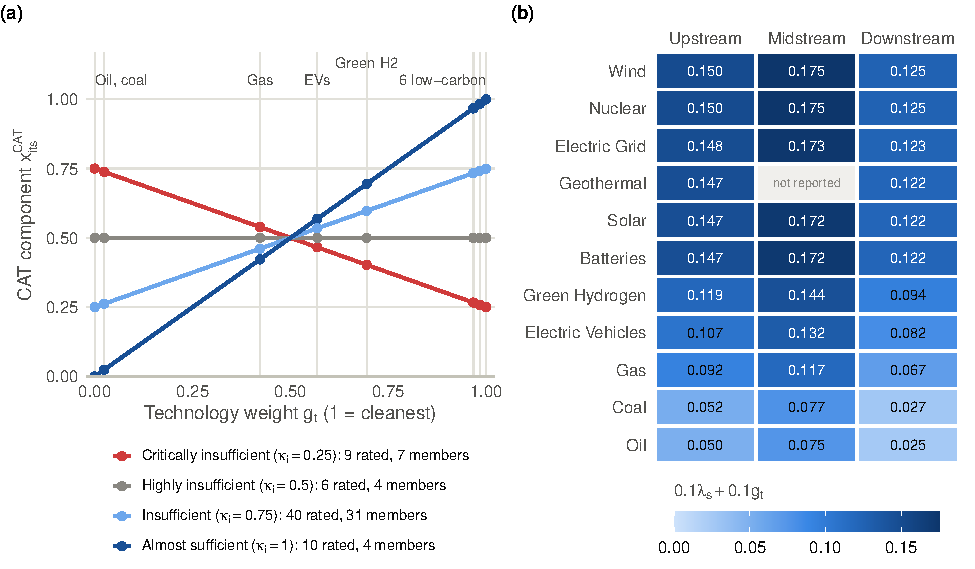
\includegraphics[width=\textwidth]{fig_si_fixed_inputs}
  \caption{The country-invariant inputs of the Strategic Index. Panel (a): the Climate Action
  Tracker component of the Policy index, $x^{\mathrm{CAT}}_{its}=\kappa_ig_t+(1-\kappa_i)(1-g_t)$,
  against the technology weight $g_t$ (IPCC life-cycle emissions, 1 = cleanest) for the four CAT
  ratings, with the eleven technologies marked on each line; the slope is $2\kappa_i-1$. The legend
  counts the countries CAT rates in each category in the final build (65 in all, 26 of them EU
  members through the EU's rating) and the coalition members among them (46 of 57: 31
  insufficient, 7 critically insufficient, 4 highly insufficient, 4 almost sufficient). Panel (b):
  the sector prior $0.1\lambda_s+0.1g_t$ that the stage weights $\lambda_s$ (Upstream 0.5, Midstream
  0.75, Downstream 0.25) and the technology weights add to the Strategic Index of every country;
  Geothermal Midstream is not a reported sector. Source: the pipeline's functions and
  \texttt{data/raw/ipcc\_ghg\_intensity.csv}, with the CAT ratings of \texttt{policy\_component\_tbl}
  in \texttt{index\_outputs.rds}; \texttt{scripts/paper/fig\_si\_fixed\_inputs.R}.}
  \label{fig:si_fixed_inputs}
\end{figure}

\subsection{Sample rules and the allied pick}\label{subsec:si_sample}

Nothing is imputed in the Strategic Index. A cell is scored only if the country has a Policy index
and both of its pillar cells are rankable under the rule of Section~\ref{sec:normalization} (the
economy is sovereign and at most half of each pillar cell's index weight is imputed); an unscored
cell stays in the output with its reason recorded. Geothermal Midstream, which has no Energy
Security pillar, is excluded by rule; a check that removes any sector whose pillar is constant
across the scored countries finds none in the final build.

\paragraph{Allied pick.}\label{subsec:si_allied} For each coalition member $i$, let $\mathcal{A}_i$
be its scored Upstream and Midstream sectors outside Geothermal and Green Hydrogen, less the Upstream
sectors barred by the endowment screen below. The allied pick is
\begin{equation}\label{eq:si_allied}
  (t,s)^{\ast}_i=\argmax_{(t,s)\in\mathcal{A}_i}\ \SI_{its}.
\end{equation}
Only the traded stages, which coalition supply chains can organise across borders, are eligible;
Geothermal and Green Hydrogen have no HS6 basket and Midstream Energy Security pillars that are
constant or concentrated at one value. The pick summarises the index for each member, EU members
included; the network design does not use it.

\paragraph{Endowment screen.} With security read as need, an economy without a resource sits at the
floor of the extraction stage's Energy Security pillar and has maximal need there. The screen makes
an Upstream stage eligible for a member's pick only if the member has recorded reserves or
production of the stage's resources (technology-level Reserves or Production greater than zero). It
is a rule of the pick, not of the index: values are unchanged and screened cells are flagged.

\subsection{Results}\label{subsec:strategic_results}

\paragraph{Coverage and basis of the Policy index.} All 57 coalition members have a Policy index, 46
on both components and 11 on the IEA component alone: Israel and Ukraine in the core and nine
partners (the Democratic Republic of the Congo, the Dominican Republic, Gabon, Ghana, Guatemala,
Malaysia, Namibia, Oman and Qatar). The two components measure different things
(Figure~\ref{fig:strategic_policy}): over the 65 economies scored on both, their Spearman
correlation is $-0.05$ across cells and $-0.02$ within a country at the median, and the composite
follows the Tracker component within a country (median 0.79) more than the IEA one (0.48). Ranking
these countries' cells on the IEA component alone gives a median within-country Spearman of 0.48
with the composite over their policy cells and 0.44 over their Strategic Index cells: the basis
matters for a country's internal ranking.

\begin{figure}[tbp]
  \centering
  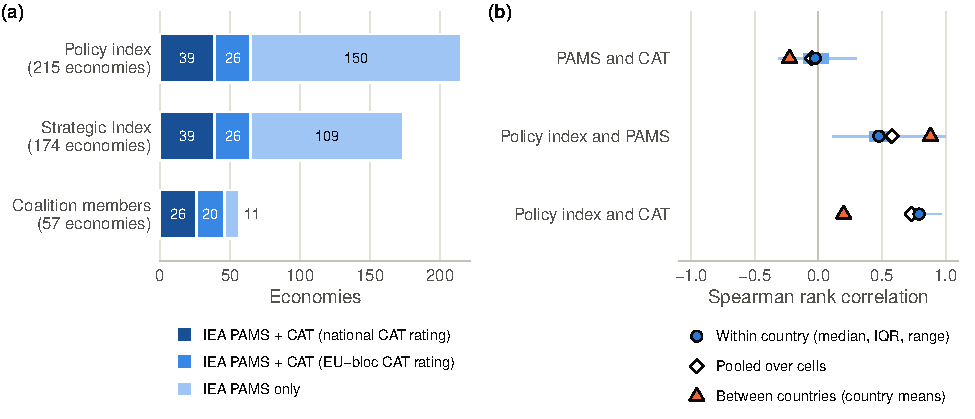
\includegraphics[width=\textwidth]{strategic_policy}
  \caption{The basis of the Policy index. Panel (a): number of economies by the components of their
  Policy index, for all economies with an index (215), the economies with a Strategic Index cell
  (174) and the coalition members (57). ``IEA PAMS + CAT'' combines the IEA Policies and Measures
  database (weight 3) with the Climate Action Tracker rating (weight 2), national or, for EU
  members, the Union's; ``IEA PAMS only'' marks economies the Tracker does not rate. Panel (b):
  Spearman correlations among the two components and the composite over the 33 cells of the 65
  economies scored on both: median, interquartile range and range of the within-country correlations
  (59 economies whose Tracker component varies across cells), pooled over cells and across country
  means. Source: \texttt{policy\_component\_tbl}, \texttt{policy\_index} in
  \texttt{index\_outputs.rds}.}
  \label{fig:strategic_policy}
\end{figure}

\paragraph{Sample and distribution.} The Strategic Index covers 3,154 cells of 174 countries in 30
sectors (Electric Grid Downstream and Geothermal Upstream have no scored cell). Of the 6,476 cells
of policy-eligible countries, 2,700 fail the rankability rule on one or both pillars and 622 lack an
Energy Security cell. Every coalition member is scored, with a median of 29 sectors. The index
(mean 0.535, standard deviation 0.082) is organised by sector far more than by country: sector fixed
effects explain 72.6 percent of its variance and country fixed effects 4.4 percent
(Figure~\ref{fig:strategic_heatmap}). The highest cells are Nuclear Upstream cells of small economies
without uranium, where Energy Security sits at a floor shared by 86 of the 174 countries and need is
maximal: Nuclear Upstream is the top sector of 62 countries, 55 of them without recorded uranium. This
construction effect of the need reading motivates the endowment screen. Green Hydrogen Midstream (34
of 40 countries at one value), Green Hydrogen Downstream, Nuclear Downstream and Batteries Downstream
also have floors; no allied pick lies in a floor cell.

\begin{figure}[tbp]
  \centering
  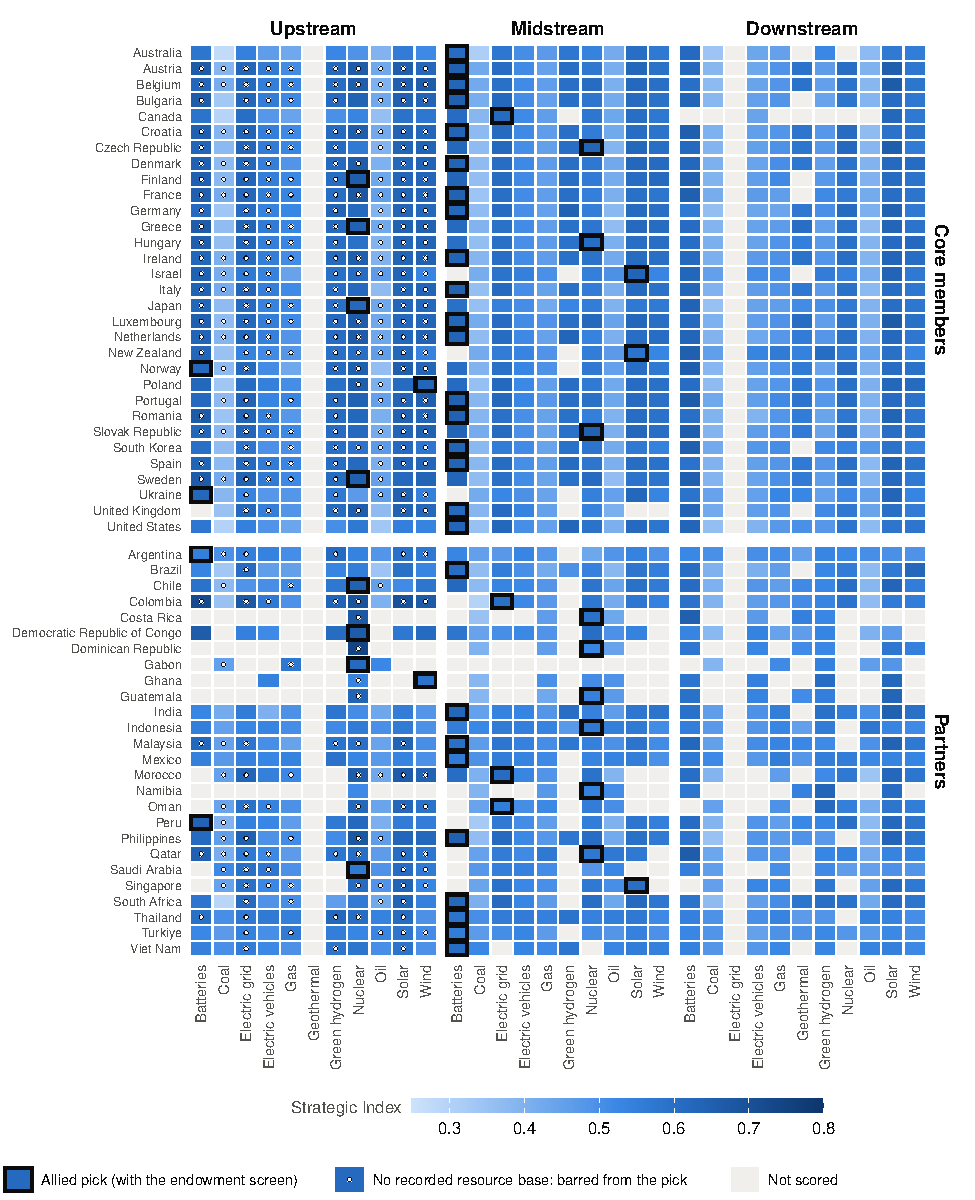
\includegraphics[width=0.94\textwidth]{strategic_heatmap}
  \caption{The Strategic Index across the coalition. Rows are the 57 members (31 core, then 26
  partners), columns the 33 technology--stage cells grouped by stage; colour is $\SI_{its}$
  (equation~\eqref{eq:si}). Grey cells are not scored (a pillar cell not rankable or missing, or
  Geothermal Midstream, excluded by rule). A dot marks an Upstream cell in which the member has no
  recorded reserves or production of the stage's resources: the endowment screen bars it from the
  pick, but its value is unchanged. The outlined cell in each row is the member's allied pick
  (equation~\eqref{eq:si_allied}). Source: \texttt{strategic\_index} in \texttt{index\_outputs.rds};
  \texttt{allied\_strategic.csv}.}
  \label{fig:strategic_heatmap}
\end{figure}

\paragraph{Decomposition.} The five terms account for 18.8 (policy), 27.6 (opportunity), 32.4
(need), 9.3 (stage) and 11.9 percent (technology) of the index level, but very different shares of
its within-country variance: on average 40.7 percent for the technology weight, 34.1 percent for
need and 32.0 percent for policy, against $-1.4$ percent for opportunity and $-5.4$ percent for the
stage weight. Opportunity moves against need (median within-country Spearman of $\EO$ and $1-\ES$
$-0.47$, negative in 164 of 167 countries; $-0.49$ and negative for all 57 coalition members), because a country's strongest opportunities tend to be
the sectors in which it is already secure; the two offset, and the ranking is set by the technology
weight, need and the policy rank (Figure~\ref{fig:strategic_decomp}).

\begin{figure}[tbp]
  \centering
  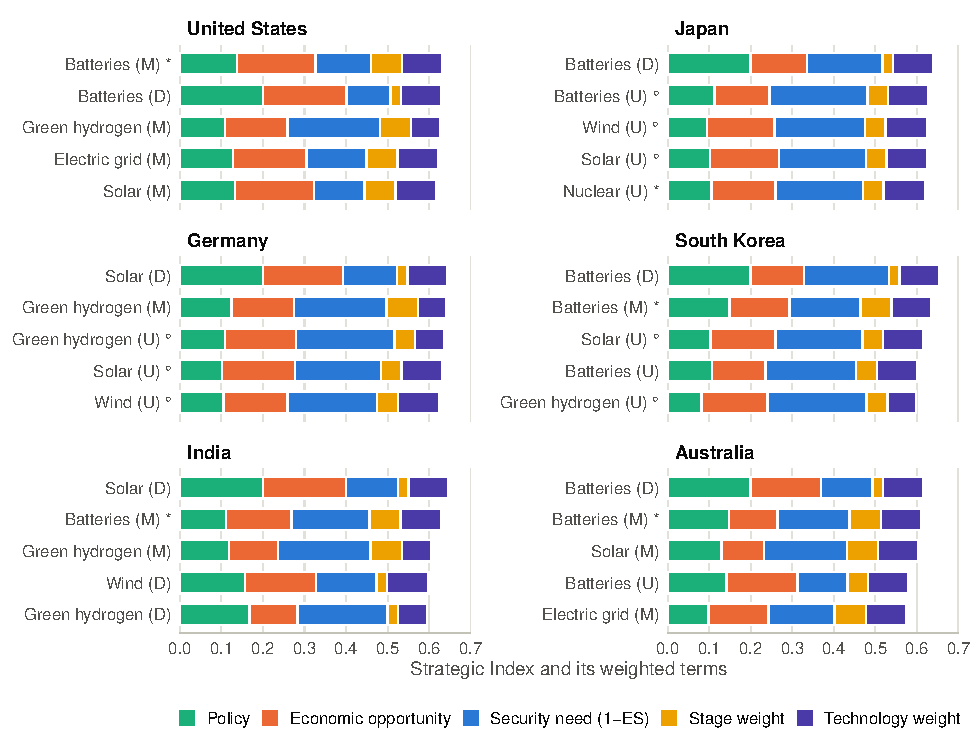
\includegraphics[width=\textwidth]{strategic_decomp}
  \caption{Decomposition of the Strategic Index for the five highest-ranked sectors of six coalition
  members. Each bar stacks the weighted terms of equation~\eqref{eq:si}: $0.2\,\POL^{*}_{its}$,
  $0.3\,\EO_{its}$, $0.3\,(1-\ES_{its})$, $0.1\,\lambda_s$ and $0.1\,g_t$; bar length is
  $\SI_{its}$. (U), (M) and (D) mark the stage; an asterisk marks the member's allied pick and a circle
  an Upstream sector barred by the endowment screen. Source: \texttt{strategic\_index} in
  \texttt{index\_outputs.rds}.}
  \label{fig:strategic_decomp}
\end{figure}

\paragraph{Allied picks.} Every member has a pick, and none is tied
(Table~\ref{tab:strategic_allied}). Batteries Midstream is the pick of 27 members (among them the
United States, Germany, Korea, India and Australia), Nuclear Midstream of nine, Nuclear Upstream of
eight, Batteries Upstream and Electric Grid Midstream of four
each, Solar Midstream of three and Wind Upstream of two (Ghana and Poland): 43 Midstream and 14
Upstream picks. The picks are sectors a member needs and supports with policy rather than sectors in
which it already competes: within a member's eligible sectors the pick ranks first on policy for 22
members and on need for 23, but on opportunity for none. The eight Nuclear Upstream picks (Chile,
the Democratic Republic of the Congo, Finland, Gabon, Greece, Japan, Saudi Arabia and Sweden) all
hold identified uranium resources, but small ones, 0.015 to 0.79 percent of world identified
resources below USD 260/kgU, and none has recorded mine production in 2019--2024. These picks are
still need-driven: a negligible resource ranks near the floor of the security pillar, so the
screen removes the no-resource artefact but not its small-resource counterpart. Requiring recorded
production rather than any reserves removes all eight Nuclear Upstream picks (seven members move
to another sector and Gabon is left without an eligible one) and the two Wind Upstream picks of
Ghana and Poland.

The picks are fragile. The median margin over the runner-up is 0.015; it is below 0.005 for 10
members (17.5 percent) and below 0.01 for 21 (36.8 percent), against a within-country standard
deviation of 0.080, so the table reports the runner-up beside each pick. The distribution also moved
during the final data revisions: in a run of 8 October, when 45 members had a pick, Electric Grid
Midstream was the pick of 17 and Batteries Midstream of 11, before completing the energy-trade file filled missing codes
of the grid basket.

The Nuclear Midstream picks of small partners are not an Energy Security floor effect. Costa Rica,
the Dominican Republic and Guatemala each have four eligible sectors, the Midstream stages of
nuclear, oil, gas and coal (Namibia these and Nuclear Upstream). The technology weight ($g_t=0.999$
for nuclear against 0.42 for gas, 0.02 for coal and 0 for oil) puts Nuclear Midstream's sector prior
0.058, 0.097 and 0.100 ahead of the three fuels, more than any other term separates pick from
runner-up, while Nuclear Midstream Energy Security is compressed around its median (interquartile
range 0.095, against 0.12--0.15 in the fossil Midstream sectors), so need adds only 0.020--0.042.

\paragraph{Picks and the network design.} The pick is a national priority read from need and
policy, not an allied assignment. Aggregated, the picks reproduce the duplication that an Allied
Industrial Base is meant to avoid: 27 members would prioritise Batteries Midstream, which the
network design of Section~\ref{sec:network} gives to nine producer nodes. Of the 27, 20 hold a
designed role in that stage, 14 of them only through the EU node, and seven (Australia, Brazil,
Mexico, the Philippines, South Africa, T\"urkiye and Viet Nam) do not. Across all members, 28 of
the 57 hold a designed share in their pick stage (the column ``Design share'' of
Table~\ref{tab:strategic_allied}), and eight (Costa Rica, the Dominican Republic, Gabon, Ghana,
Guatemala, New Zealand, T\"urkiye and Ukraine) produce nothing in the design.

% Generated by scripts/paper/fig_strategic.R -- do not edit by hand.
\begingroup
\singlespacing\scriptsize
\setlength{\tabcolsep}{2.9pt}
\setlength{\LTcapwidth}{\textwidth}
\begin{longtable}{@{}l l S[table-format=1.3] l S[table-format=1.4] c l c c@{}}
\caption{Allied strategic selection: pick, runner-up, margin and robustness of the pick}
\label{tab:strategic_allied}\\
\toprule
 & & & & & & & \multicolumn{2}{c@{}}{\makecell{Same pick\\under}}\\
\cmidrule(l){8-9}
Member & Pick & {$\SI$} & Runner-up & {Margin} & \makecell{AIB\\coalitions} & \makecell[l]{Pick without\\the screen} & (1) & (2)\\
\midrule
\endfirsthead
\multicolumn{9}{@{}l}{\small\textbf{Table \thetable:} continued}\\
\toprule
 & & & & & & & \multicolumn{2}{c@{}}{\makecell{Same pick\\under}}\\
\cmidrule(l){8-9}
Member & Pick & {$\SI$} & Runner-up & {Margin} & \makecell{AIB\\coalitions} & \makecell[l]{Pick without\\the screen} & (1) & (2)\\
\midrule
\endhead
\midrule
\multicolumn{9}{r@{}}{\textit{Continued on the next page}}\\
\endfoot
\bottomrule
\endlastfoot
\multicolumn{9}{@{}l}{\textit{Core members (31 of 31 with a pick)}}\\
Australia & Batteries (M) & 0.610 & Solar (M) & 0.0063 & 1 & same & -- & $\checkmark$ \\
Austria & Batteries (M) & 0.647 & Solar (M) & 0.0187 & 2 & Nuclear (U) & -- & $\checkmark$ \\
Belgium & Batteries (M) & 0.634 & Solar (M) & 0.0142 & -- & Wind (U) & -- & $\checkmark$ \\
Bulgaria & Batteries (M) & 0.651 & Nuclear (U) & 0.0101 & -- & Batteries (U) & -- & -- \\
Canada & Electric grid (M) & 0.615 & Batteries (M) & 0.0052 & -- & same & -- & -- \\
Croatia & Batteries (M) & 0.638 & Electric grid (M) & 0.0235 & -- & Nuclear (U) & -- & $\checkmark$ \\
Czech Republic & Nuclear (M) & 0.632 & Solar (M) & 0.0071 & -- & Wind (U) & -- & $\checkmark$ \\
Denmark & Batteries (M) & 0.636 & Solar (M) & 0.0109 & -- & Nuclear (U) & -- & $\checkmark$ \\
Finland & Nuclear (U) & 0.658 & Batteries (M) & 0.0245 & -- & same & -- & $\checkmark$ \\
France & Batteries (M) & 0.642 & Electric grid (M) & 0.0421 & 1 & Nuclear (U) & -- & $\checkmark$ \\
Germany & Batteries (M) & 0.623 & Nuclear (U) & 0.0073 & 2 & Solar (U) & -- & -- \\
Greece & Nuclear (U) & 0.643 & Batteries (M) & 0.0252 & -- & Batteries (U) & -- & $\checkmark$ \\
Hungary & Nuclear (M) & 0.606 & Wind (M) & 0.0015 & -- & Batteries (U) & -- & -- \\
Ireland & Batteries (M) & 0.636 & Solar (M) & 0.0244 & -- & Nuclear (U) & -- & $\checkmark$ \\
Israel$^{\dagger}$ & Solar (M) & 0.636 & Electric grid (M) & 0.0487 & -- & Batteries (U) & -- & $\checkmark$ \\
Italy & Batteries (M) & 0.639 & Nuclear (U) & 0.0181 & -- & Batteries (U) & -- & -- \\
Japan & Nuclear (U) & 0.620 & Batteries (M) & 0.0231 & -- & Batteries (U) & -- & $\checkmark$ \\
Luxembourg & Batteries (M) & 0.628 & Solar (M) & 0.0005 & -- & Nuclear (U) & -- & $\checkmark$ \\
Netherlands & Batteries (M) & 0.635 & Electric grid (M) & 0.0242 & 1 & Nuclear (U) & -- & $\checkmark$ \\
New Zealand & Solar (M) & 0.587 & Electric grid (M) & 0.0269 & -- & Batteries (U) & -- & $\checkmark$ \\
Norway & Batteries (U) & 0.618 & Batteries (M) & 0.0148 & -- & Solar (U) & -- & $\checkmark$ \\
Poland & Wind (U) & 0.633 & Batteries (U) & 0.0089 & -- & Nuclear (U) & -- & $\checkmark$ \\
Portugal & Batteries (M) & 0.644 & Nuclear (U) & 0.0007 & -- & Wind (U) & -- & -- \\
Romania & Batteries (M) & 0.643 & Nuclear (U) & 0.0195 & -- & Batteries (U) & -- & -- \\
Slovak Republic & Nuclear (M) & 0.644 & Batteries (M) & 0.0054 & -- & Wind (U) & -- & -- \\
South Korea & Batteries (M) & 0.635 & Batteries (U) & 0.0348 & 2 & same & -- & $\checkmark$ \\
Spain & Batteries (M) & 0.636 & Nuclear (U) & 0.0200 & -- & same & -- & -- \\
Sweden & Nuclear (U) & 0.649 & Wind (U) & 0.0145 & -- & Batteries (U) & -- & $\checkmark$ \\
Ukraine$^{\dagger}$ & Batteries (U) & 0.624 & Solar (M) & 0.0018 & -- & Solar (U) & -- & $\checkmark$ \\
United Kingdom & Batteries (M) & 0.617 & Electric grid (M) & 0.0042 & 1 & Nuclear (U) & -- & $\checkmark$ \\
United States & Batteries (M) & 0.632 & Electric grid (M) & 0.0096 & 3 & same & -- & $\checkmark$ \\
\midrule
\multicolumn{9}{@{}l}{\textit{Partners (26 of 26 with a pick)}}\\
Argentina & Batteries (U) & 0.551 & Solar (M) & 0.0114 & -- & Solar (U) & -- & -- \\
Brazil & Batteries (M) & 0.606 & Solar (U) & 0.0088 & -- & Electric grid (U) & -- & -- \\
Chile & Nuclear (U) & 0.645 & Batteries (M) & 0.0251 & -- & same & -- & $\checkmark$ \\
Colombia & Electric grid (M) & 0.597 & Solar (M) & 0.0195 & -- & Batteries (U) & $\checkmark$ & $\checkmark$ \\
Costa Rica & Nuclear (M) & 0.592 & Gas (M) & 0.1285 & -- & Nuclear (U) & $\checkmark$ & $\checkmark$ \\
Democratic Republic of Congo$^{\dagger}$ & Nuclear (U) & 0.664 & Batteries (U) & 0.0053 & -- & same & -- & $\checkmark$ \\
Dominican Republic$^{\dagger}$ & Nuclear (M) & 0.532 & Gas (M) & 0.0733 & -- & Nuclear (U) & $\checkmark$ & -- \\
Gabon$^{\dagger}$ & Nuclear (U) & 0.616 & Oil (U) & 0.0921 & -- & same & -- & -- \\
Ghana$^{\dagger}$ & Wind (U) & 0.589 & Electric vehicles (U) & 0.0469 & -- & same & -- & $\checkmark$ \\
Guatemala$^{\dagger}$ & Nuclear (M) & 0.546 & Oil (M) & 0.0768 & -- & Nuclear (U) & $\checkmark$ & -- \\
India & Batteries (M) & 0.628 & Wind (M) & 0.0437 & 1 & same & -- & $\checkmark$ \\
Indonesia & Nuclear (M) & 0.568 & Solar (M) & 0.0007 & 1 & same & -- & -- \\
Malaysia$^{\dagger}$ & Batteries (M) & 0.596 & Solar (M) & 0.0109 & 1 & Solar (U) & -- & $\checkmark$ \\
Mexico & Batteries (M) & 0.564 & Electric grid (M) & 0.0064 & -- & same & -- & -- \\
Morocco & Electric grid (M) & 0.609 & Batteries (M) & 0.0014 & -- & Solar (U) & $\checkmark$ & -- \\
Namibia$^{\dagger}$ & Nuclear (M) & 0.542 & Nuclear (U) & 0.0223 & -- & same & -- & -- \\
Oman$^{\dagger}$ & Electric grid (M) & 0.556 & Nuclear (M) & 0.0011 & -- & Solar (U) & -- & -- \\
Peru & Batteries (U) & 0.639 & Nuclear (U) & 0.0189 & -- & same & -- & $\checkmark$ \\
Philippines & Batteries (M) & 0.648 & Solar (U) & 0.0190 & -- & Nuclear (U) & -- & -- \\
Qatar$^{\dagger}$ & Nuclear (M) & 0.573 & Oil (M) & 0.0031 & -- & Batteries (U) & -- & -- \\
Saudi Arabia & Nuclear (U) & 0.567 & Electric grid (M) & 0.0156 & -- & Solar (U) & -- & -- \\
Singapore & Solar (M) & 0.601 & Electric grid (M) & 0.0084 & -- & Solar (U) & -- & -- \\
South Africa & Batteries (M) & 0.620 & Solar (M) & 0.0019 & 1 & Solar (U) & -- & $\checkmark$ \\
Thailand & Batteries (M) & 0.587 & Solar (M) & 0.0182 & -- & Solar (U) & -- & -- \\
Turkiye & Batteries (M) & 0.556 & Solar (M) & 0.0124 & -- & Solar (U) & -- & -- \\
Viet Nam & Batteries (M) & 0.606 & Nuclear (U) & 0.0273 & 2 & same & -- & -- \\
\midrule
\multicolumn{6}{@{}l}{Members with the same pick (of 57)} & 16 & 5 & 31\\
\end{longtable}
\vspace{-6pt}\noindent
\textit{Notes:} For each coalition member with a Strategic Index, the pick is the Upstream or Midstream sector outside Geothermal and Green Hydrogen with the highest index (equation~\eqref{eq:si_allied}), after the endowment screen bars Upstream sectors in which the member has no recorded reserves or production; the runner-up is the second-highest such sector and the margin the difference between their indices; (U) Upstream, (M) Midstream. No member has a tie. AIB coalitions counts the Sectoral Compacts of Section~\ref{sec:network} with a node in the pick stage whose exact minimum coalition includes the member (-- if none). ``Pick without the screen'' is the pick when the endowment screen is switched off (``same'' if unchanged); the index values are the same in both cases. Columns (1) and (2) mark whether the pick, with the screen, is unchanged when the index is recomputed on the same cells (1) with security strength $\ES$ in place of need $1-\ES$ and (2) without the stage and technology weights. All 57 members have a pick. $^{\dagger}$\,Policy index on IEA PAMS alone (no CAT rating; 11 members); the other members' Policy index combines IEA PAMS and CAT. Source: \texttt{index\_outputs.rds} and \texttt{allied\_strategic.csv} of the final run, which the script reproduces; \texttt{scripts/paper/fig\_strategic.R}.\par
\endgroup
\medskip


\paragraph{The endowment screen.} Of the 998 scored Upstream cells in the screened technologies,
669 have no recorded resource base (306 of the coalition's 509). The screen changes 41 of the 57
picks (Figure~\ref{fig:strategic_screen}): without it 47 picks would be Upstream (Nuclear 17,
Batteries 12, Solar 12, Wind 5 and Electric Grid 1), many in members without the resource, such as Nuclear Upstream for
France and the United Kingdom. The index forgone is small for most members (median 0.026; largest
for the Dominican Republic, 0.216). An economy cannot become an allied supplier of a resource for
which it has no recorded reserves or production.

\begin{figure}[tbp]
  \centering
  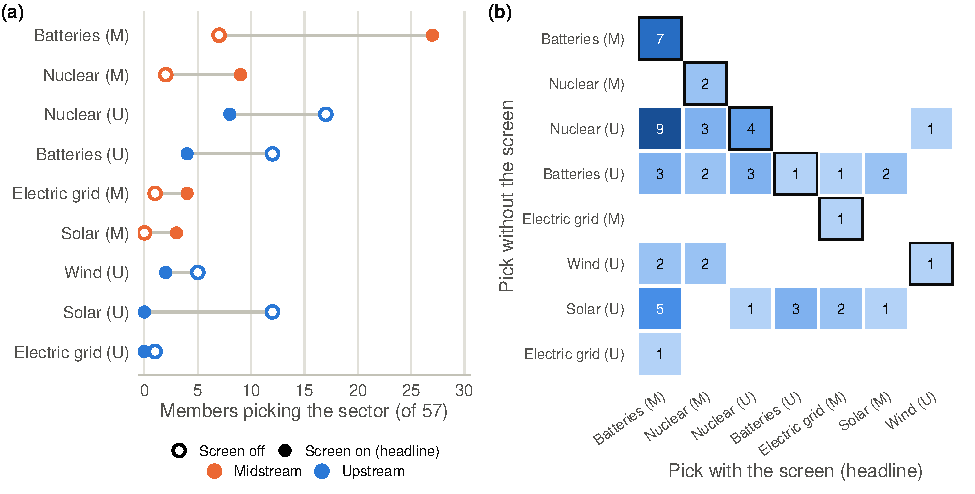
\includegraphics[width=\textwidth]{strategic_screen}
  \caption{Allied picks with and without the endowment screen. Panel (a): number of the 57 members
  whose pick is each sector, with the screen (filled, the headline) and without it (open); colour is
  the stage. Panel (b): transition between the two selections; each tile counts the members whose
  pick without the screen is the row and with it the column; outlined diagonal tiles are unchanged
  picks (16 members). Index values are the same in both selections; the screened selection equals
  \texttt{allied\_strategic.csv}. Source: \texttt{strategic\_index} in \texttt{index\_outputs.rds};
  \texttt{select\_allied\_strategic\_sectors()} with the screen on and off.}
  \label{fig:strategic_screen}
\end{figure}

\paragraph{The security sign and other normative choices.} Reading security as strength, $\ES$ in
place of $1-\ES$, gives an index that agrees only weakly with the headline
(Figure~\ref{fig:strategic_sign}): the median within-member Spearman correlation is 0.36, only 5 of
the 57 picks survive, and picks move to Nuclear Midstream (28), Gas Midstream (10) and Electric Grid
Midstream (7). The sign is the most consequential normative choice: the need reading asks where an
economy should build capability to reduce its exposure, the strength reading where it can build on
capability it has. The other choices keep median within-member correlations of 0.88--0.96 but
change many picks. Of the 57 members, 31 keep their pick without the stage and technology priors, 30
without the policy term, 20 when opportunity and need are ranked within the country, and 34 when the
October 2026 NIPO component is added back (27 of the 50 members with NIPO data); policy from IEA
PAMS alone keeps 45 (34 of the 46 members scored on both components). The headline pick stays in
the variant's top three for 86 to 96 percent of members. Requiring both policy
components removes the 11 members scored on the IEA component alone and leaves the other cells
unchanged. A member's sector ordering is thus robust to these choices, but its single pick is not
(Online Appendix~\ref{oa:strategic}; Section~\ref{sec:robustness}).

\begin{figure}[tbp]
  \centering
  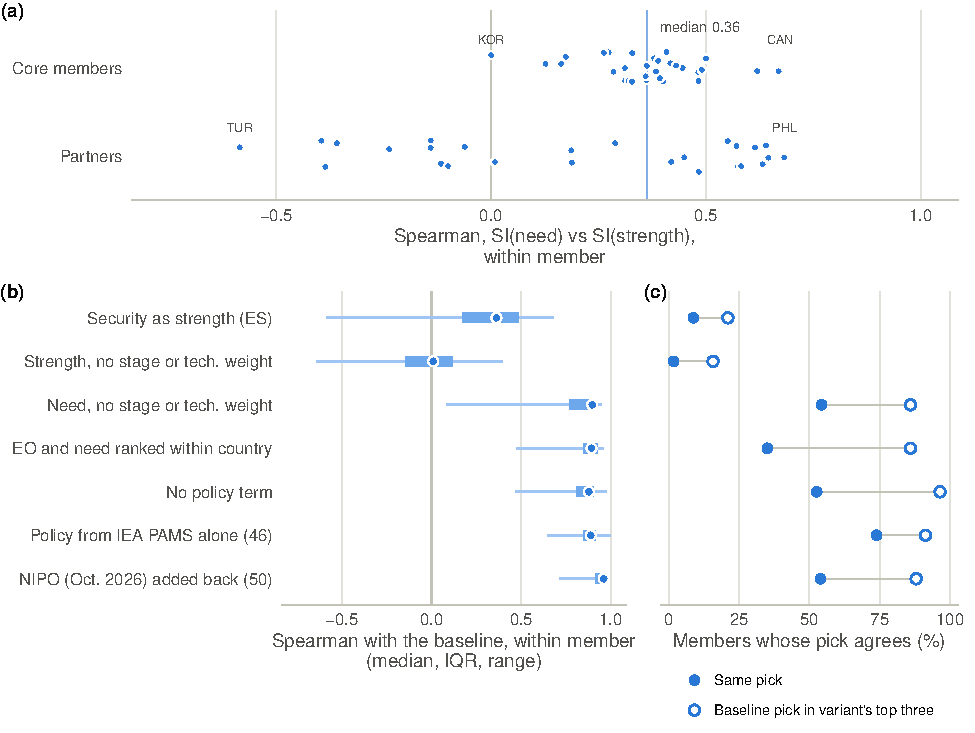
\includegraphics[width=\textwidth]{strategic_sign}
  \caption{Sensitivity of the Strategic Index to its normative choices, coalition members. Panel
  (a): within-member Spearman correlation between the headline index (security as need, $1-\ES$) and
  the index with security as strength ($\ES$), all other terms unchanged; one point per member, by
  tier, median marked. Panel (b): within-member Spearman correlation of each variant with the
  headline (median, interquartile range and range): strength; strength without the stage and
  technology weights; need without those weights; opportunity and need ranked within the country; no
  policy term; policy from the IEA component alone (46 members scored on both); the October 2026 NIPO
  component added back (50 members with NIPO data). Panel (c): share of members whose pick is
  unchanged (filled) and whose headline pick is among the variant's top three (open); the IEA-alone and
  NIPO rows are shares of the 46 and 50 members whose index the variant changes, and over all 57
  members 45 and 34 picks are unchanged (Table~\ref{tab:robustness_picks}). All variants
  keep the endowment screen and the headline cells. Source: \texttt{index\_outputs.rds}; the NIPO
  component of the October 2026 run.}
  \label{fig:strategic_sign}
\end{figure}

% =============================================================================
% Section 9. Bilateral partnership indices
% Specification: R/themes/partnership_strength/{partnership_strength_helpers,safer_friendshore,
% cm_fdi,prosperous_opportunity,stronger_development,psi_composite}.R,
% R/indices/build_partnership_strength_index.R, scripts/15_build_partner_themes.R,
% scripts/25_build_partner_indices.R, config/weights.yml (psi, partnership_*_components),
% config/partnership.yml (trade mirror, conduits, cm_fdi), config/rankability.yml.
% Numbers: paper/results/bilateral.json (final rerun of 2026-10-12); figures and tables:
% scripts/paper/fig_bilateral.R. Further detail: sections/oa_bilateral.tex (oa:bilateral).
% =============================================================================
\section{Bilateral partnership indices}\label{sec:bilateral}

The choice of partner trades the security of trusted suppliers against the efficiency cost of
narrowing the supplier set \citep{yellen2022remarks,aiyar2023geoeconomic,gopinath2025changing,
javorcik2024economic,grossman2023supply}, and sourcing is already being reallocated across partners
\citep{alfaro2023global,freund2024us}. Its unit is the pair of countries. This section builds three
bilateral pillars and a composite: the
\emph{Friendshore} index $\FS$ rates partner $j$ as a supplier of $(t,s)$ to economy $i$; the
\emph{Partnership Opportunity} index $\PO$ rates $j$ as a market for $i$'s exports; the
\emph{Development Potential} index $\DP$ rates $j$ alone as a development partner; and the
\emph{Partnership Strength Index} $\PSI$ combines them (Table~\ref{tab:bilateral_pillars}). The
network design (Section~\ref{sec:network}) uses the dyad-level $\FS$ and $\PO$ and the partner-level
$\DP$, not the $\PSI$.

\begin{table}[tbp]
\centering
\begin{threeparttable}
\caption{The bilateral pillars: units, direction, components and weights}
\label{tab:bilateral_pillars}
\footnotesize
\begin{tabularx}{\textwidth}{@{}>{\raggedright\arraybackslash}p{2.2cm}
  >{\raggedright\arraybackslash}X >{\raggedright\arraybackslash}X
  >{\raggedright\arraybackslash}X@{}}
\toprule
 & Friendshore ($\FS$) & Partnership Opportunity ($\PO$) & Development Potential ($\DP$)\\
\midrule
Unit & dyad $\dyad$ & dyad $\dyad$ & partner $(j,t,s)$\\
Reporter $i$ & importer, sourcing $(t,s)$ & exporter of $(t,s)$ & none\\
Partner $j$ & candidate supplier & candidate export market & non-high-income economy\\
Components (weight) &
  $\tau^{M}_{ijts}$ imports from $j$ (2); $\nu_{its}$ reporter need (2); $e_{jts}$ partner $\EO$
  rank (2); $o_{ijts}$ outward investment in $j$ (2); $A_{ij}$ UNGA alignment (2); $1-\chi_{jt}$
  Chinese-parent exposure (1; four Midstream cells); reporter $\EO$ rank (0) &
  $\tau^{X}_{ijts}$ exports to $j$ (3); $\varepsilon_{its}$ reporter $\EO$ rank (3);
  $\eta_{jts}$ partner $\ES$ need (1) &
  eight partner components, weights $1,1,1,1,1.5,1.5,2,1$ (Table~\ref{tab:dp_components})\\
Climate penalty & $0.10\,(1-g_t)(\mathrm{CPI}_i+\mathrm{CPI}_j)$ & $0.05\,(1-g_t)\,\mathrm{CPI}_j$
  & none\\
Final transform & ${\Scurve}[\cdot]_{ts}$ over dyads, after flooring at 0 & ${\Scurve}[\cdot]_{ts}$
  over dyads, after flooring at 0 & ${\Scurve}[\cdot]_{ts}$ over partners\\
Summary to $\PSI$ & best five $(t,s)$ per dyad; mean over the core reporters & best five $(t,s)$
  per dyad; mean over the core reporters & best five $(t,s)$ per partner\\
$\PSI$ weight & $0.4$ & $0.4$ & $0.2$\\
\bottomrule
\end{tabularx}
\begin{tablenotes}[flushleft]\footnotesize
\item \textit{Notes:} Weights from \texttt{config/weights.yml}; within each pillar they are
renormalized over the components observed (equation~\eqref{eq:bilateral_acmean}). The $\FS$ penalty
coefficient (0.10 per side) is fixed in code, the $\PO$ coefficient configured. $g_t$ is the
technology emission weight of equation~\eqref{eq:ghg_index}, $\mathrm{CPI}$ the Climate Action
Tracker rating. In Batteries, Electric Vehicles, Solar and Wind Midstream $o_{ijts}$ is the CM-FDI
project tie and $\chi_{jt}$ is defined; elsewhere $o_{ij}$ is the IMF position and $\chi$ is absent.
\end{tablenotes}
\end{threeparttable}
\end{table}

% -----------------------------------------------------------------------------
\subsection{Dyads, trade and shared building blocks}\label{subsec:bilateral_dyads}

A dyad $\dyad$ pairs reporter $i$ and partner $j\neq i$, among 219 economies, in a headline
technology $t$ and stage $s$. In $\FS_{ijts}$ the reporter is the importer and $j$ the candidate
supplier; in $\PO_{ijts}$ the reporter is the exporter and $j$ the candidate market. Both rate $j$
from $i$'s side, so a supply edge from producer $p$ to consumer $c$ is read as $\FS_{cpts}$ and
$\PO_{pcts}$ (Section~\ref{sec:network}). ${\Scurve}[x]_{g}$ is the S-curve of
Section~\ref{sec:normalization} within each cell of grouping $g$ ($ts$: all dyads of a cell; $its$:
reporter $i$'s partners in the cell; $i$: all units of reporter $i$). Missing components are dropped
and the weights renormalized,
\begin{equation}\label{eq:bilateral_acmean}
  \mathcal{A}_{\bm w}(x_1,\dots,x_C)=\frac{\sum_{c} w_c\,x_c\,\1\{x_c\ \text{observed}\}}
  {\sum_{c} w_c\,\1\{x_c\ \text{observed}\}},
\end{equation}
so a missing component is never scored as zero.

\paragraph{Bilateral trade.}\label{subsec:bilateral_blocks} Trade comes from the all-reporter
Comtrade dyads for 2020 and 2024 \citep{uncomtrade}: the importer's own declaration where it reports
the cell, otherwise the exporter's mirror declaration times the CIF/FOB factor 1.06; a reporter that
declares no trade with a partner records a zero, and non-reporting economies enter only through
their partners' declarations. With $H_{ts}$ the HS6 basket of the cell (Section~\ref{sec:data}),
the cell flow is
\begin{equation}\label{eq:bilateral_trade_value}
  M^{y}_{ijts}=\sum_{h\in H_{ts}} m^{y}_{ijh},
\end{equation}
a product in several baskets counting in each. Among dyads that trade, the 2024 level $L$ and the
growth since 2020 $G$ are ranked within the cell and combined 2:1, then re-ranked among the
reporter's own suppliers,
\begin{equation}\label{eq:bilateral_trade_index}
  \tilde\tau^{M}_{ijts}=\mathcal{A}_{(2,1)}\bigl({\Scurve}[L]_{ts},\,{\Scurve}[G]_{ts}\bigr),
  \qquad
  \tau^{M}_{ijts}={\Scurve}\bigl[\tilde\tau^{M}\bigr]_{its},
\end{equation}
so that $\tau^{M}_{ijts}$ measures $j$'s place among $i$'s sources. Recorded zeros form one tie block
below every trading partner; a dyad with no observed 2024 flow takes the cell mean; the 15 cells
without a basket carry no trade information. The export component $\tau^{X}_{ijts}$ is built the
same way from $i$'s exports.

\paragraph{Climate penalty.} Each economy carries a Climate Action Tracker rating $\mathrm{CPI}_i$
\citep{cat2026ratings} (0.25 to 1; EU members take the EU's, unrated economies the median, 0.75).
The penalty is proportional to $(1-g_t)\,\mathrm{CPI}$, with $g_t$ the technology weight of
equation~\eqref{eq:ghg_index}. Because $g_t$ is constant within a cell, it re-orders dyads within
carbon-intensive technologies by the parties' climate ambition \citep{clausing2023carbon} rather than
lowering those technologies against clean ones.

% -----------------------------------------------------------------------------
\subsection{The Friendshore index}\label{subsec:friendshore}

Friendshore asks how good a supplier $j$ is for $i$ in $(t,s)$. Besides the import component it
has the reporter's need, ranked among its own cells, and the partner's capability, ranked across
countries,
\begin{equation}\label{eq:fs_need}
  \nu_{its}=1-{\Scurve}[\ES]_{i}(i,t,s),\qquad e_{jts}={\Scurve}[\EO]_{ts}(j,t,s),
\end{equation}
so that $\nu$ identifies which technologies $i$ should friendshore, not which countries most need
to. The dyadic alignment $A_{ij}$ of equation~\eqref{eq:coalition_dyadic} enters as it is, without
ranking.

\paragraph{Outward investment.} An outward position reveals an ownership or financing link that gives
the investor a stake in the partner's capacity. Outside four cells, $o_{ij}$ uses the reporter's
outward direct-investment debt positions in the IMF Direct Investment Positions \citep{imf2026dip},
averaged over 2020--2024 ($\bar D_{ij}$); positions involving 16 conduit financial centres,
dominated by pass-through capital \citep{damgaard2024real}, are unobserved on both sides. With $Y$
the 2023 GDP,
\begin{equation}\label{eq:outbound}
  \tilde o_{ij}=
  \begin{cases}
    \mathcal{A}_{(1,1,1)}\bigl({\Scurve}[\bar D],\ {\Scurve}[\bar D/Y_j],\ {\Scurve}[(\bar D/Y_i)/Y_j]\bigr)
      & \text{if } \bar D_{ij}>0,\\[2pt]
    0 & \text{if } \bar D_{ij}\le 0,
  \end{cases}
  \qquad
  o_{ij}={\Scurve}[\tilde o]_{i}.
\end{equation}
An absent record is missing, not zero. In Batteries, Electric Vehicles, Solar and Wind Midstream the
tie $o_{ijts}$ comes instead from the CM-FDI database of cross-border clean-technology manufacturing
projects \citep{bandara2026cmfdi}: the projects of parents headquartered in $i$ located in $j$,
ranked on attributed counts and disclosed capital within the cell and then within the reporter.

\paragraph{Chinese-parent exposure.} For supplier $j$ and technology $t$ in the same four cells,
$\chi_{jt}$ is the share of $j$'s foreign-invested manufacturing owned by parents headquartered in
China, Hong Kong or Macao: capital-weighted where capital is disclosed and by count otherwise, half
of a joint venture attributed to the listed parent, defined only where $j$ hosts at least two
projects, and set to one for China, Hong Kong and Macao. It enters as $1-\chi_{jt}$, so a supplier
whose foreign-invested capacity belongs to Chinese parents scores lower.

\paragraph{Composite and index.} With the reporter's own $\EO$ rank carried at weight zero,
\begin{equation}\label{eq:fs_raw}
  \tilde F_{ijts}=\mathcal{A}_{\bm w^{\FS}}\bigl(\tau^{M}_{ijts},\,\nu_{its},\,e_{jts},\,o_{ijts},\,
  A_{ij},\,1-\chi_{jt}\bigr),\qquad \bm w^{\FS}=(2,2,2,2,2,1),
\end{equation}
\begin{equation}\label{eq:fs_penalty}
  \pi^{\FS}_{ijt}=0.10\,(1-g_t)\,(\mathrm{CPI}_i+\mathrm{CPI}_j),
\end{equation}
\begin{equation}\label{eq:fs_index}
  \FS_{ijts}={\Scurve}\bigl[\max\bigl(0,\ \tilde F-\pi^{\FS}\bigr)\bigr]_{ts}.
\end{equation}
The index rewards a match between the reporter's weaknesses and the partner's strengths, backed by
revealed ties and political alignment.

% -----------------------------------------------------------------------------
\subsection{The Partnership Opportunity index}\label{subsec:partnership_opportunity}

A market is worth more to an exporter when the exporter is competitive in the technology, already
sells there, and the market's insecurity signals demand for new supply. With the reporter's and the
market's cross-country ranks,
\begin{equation}\label{eq:po_components}
  \varepsilon_{its}={\Scurve}\bigl[{\Scurve}[\EO]_{ts}(i,t,s)\bigr]_{ts},\qquad
  \eta_{jts}={\Scurve}\bigl[1-{\Scurve}[\ES]_{ts}(j,t,s)\bigr]_{ts},
\end{equation}
\begin{equation}\label{eq:po_index}
  \tilde P_{ijts}=\mathcal{A}_{(3,3,1)}\bigl(\tau^{X}_{ijts},\,\varepsilon_{its},\,\eta_{jts}\bigr),
  \qquad
  \pi^{\PO}_{jt}=0.05\,(1-g_t)\,\mathrm{CPI}_j,
  \qquad
  \PO_{ijts}={\Scurve}\bigl[\max\bigl(0,\ \tilde P-\pi^{\PO}\bigr)\bigr]_{ts}.
\end{equation}
Unlike the Friendshore need term, $\eta_{jts}$ compares the market's insecurity with that of other
markets. The penalty falls on the market's climate policy only.

% -----------------------------------------------------------------------------
\subsection{The Development Potential index}\label{subsec:development_potential}

Development Potential describes partner $j$ alone: its enabling environment, energy-security need,
economic opportunity, the official development assistance it receives in each stage, and its energy
use (Table~\ref{tab:dp_components}). It is defined for the 132 partners that the World Bank does not
classify as high income,
\begin{equation}\label{eq:dp_index}
  \widetilde D_{jts}=\mathcal{A}_{\bm w^{\DP}}\bigl(d^{(1)}_{jts},\dots,d^{(8)}_{jts}\bigr),\qquad
  \bm w^{\DP}=(1,1,1,1,1.5,1.5,2,1),\qquad
  \DP_{jts}={\Scurve}\bigl[\widetilde D\bigr]_{ts},
\end{equation}
ranked across eligible partners within the cell. Only need, opportunity and stage aid vary across a
partner's cells, so they decide which cells its best-five summary selects. Online
Appendix~\ref{oa:bilateral} gives the 40-series WDI basket, the aid measure and the orientation
choices.

\begin{table}[tbp]
\centering
\begin{threeparttable}
\caption{Components of the Development Potential index}
\label{tab:dp_components}
\footnotesize
\begin{tabularx}{\textwidth}{@{}l l >{\raggedright\arraybackslash}X c@{}}
\toprule
Component & Varies by & Construction & Weight\\
\midrule
$d^{(1)}$ development index & $j$ & S-curve across economies of the mean of the observed
  S-curved WDI series of a 40-series basket (2022--2024 averages; 13 inverted) & 1\\
$d^{(2)}$ business environment & $j$ & S-curve of the Doing Business score (2019, last release) & 1\\
$d^{(3)}$ investment environment & $j$ & S-curve of $(d^{(1)}+d^{(2)})/2$ & 1\\
$d^{(4)}$ energy-security need & $j,t,s$ & $1-\ES_{jts}$ & 1\\
$d^{(5)}$ economic opportunity & $j,t,s$ & $\EO_{jts}$ & 1.5\\
$d^{(6)}$ stage aid & $j,s$ & S-curve of ODA disbursements to the stage's sector (OECD CRS) & 1.5\\
$d^{(7)}$ stage aid intensity & $j,s$ & the same per unit of 2023 GDP & 2\\
$d^{(8)}$ energy use & $j$ & S-curve of energy use per capita & 1\\
\bottomrule
\end{tabularx}
\begin{tablenotes}[flushleft]\footnotesize
\item \textit{Notes:} Weights from \texttt{config/weights.yml}
(\texttt{partnership\_development\_components}). Stage aid: industry to Midstream, energy to
Downstream, mineral resources and mining net of coal and upstream oil and gas to Upstream. A
partner without a record of a component has it dropped, not scored as zero. Sources and the WDI
basket: Online Appendix~\ref{oa:bilateral}.
\end{tablenotes}
\end{threeparttable}
\end{table}

% -----------------------------------------------------------------------------
\subsection{From dyads to partners: best-five summaries and the PSI}\label{subsec:psi}

The $\PSI$ collapses technology and stage before reporters. For a dyad, the summary of a pillar is
the mean of its five highest cells,
\begin{equation}\label{eq:top5}
  T^{v}_{ij}=\frac{1}{K_{ij}}\sum_{k=1}^{K_{ij}}v_{ij(k)},\qquad K_{ij}=\min(5,\,n_{ij}),
\end{equation}
and $T^{\DP}_{j}$ is the same over the partner's own cells. Partnerships in energy technologies are
sector-specific, and an average over all cells would penalize a partner that is strong in a few
technologies; the summary is therefore optimistic by design. With $R$ the set of reporters whose
view is taken, the category scores and the index are
\begin{equation}\label{eq:psi_category}
  C^{k}_j=\frac{1}{|R^{k}_j|}\sum_{i\in R^{k}_j}T^{k}_{ij}\ \ (k=\FS,\PO;\ R^{k}_j\subseteq R),
  \qquad C^{\DP}_j=T^{\DP}_{j},
\end{equation}
\begin{equation}\label{eq:psi}
  \PSI_j=\frac{\sum_{k\in K_j}w_k\,C^{k}_j}{\sum_{k\in K_j}w_k},\qquad
  (w_{\FS},w_{\PO},w_{\DP})=(0.4,\,0.4,\,0.2),
\end{equation}
where $K_j$ is the set of categories observed for $j$ (a high-income partner has no $\DP$). The
headline takes the viewpoint of the coalition's core: $R$ is the 31 core members
(Section~\ref{sec:coalition}), so that $\PSI_j$ is $j$'s value to the economies that anchor the
coalition; the full-coalition (57 reporters) and world views are alternatives. For one pair,
\begin{equation}\label{eq:psi_dyad}
  \PSI_{ij}=\mathcal{A}_{(0.4,0.4,0.2)}\bigl(T^{\FS}_{ij},\,T^{\PO}_{ij},\,T^{\DP}_{j}\bigr),
  \qquad i\neq j,
\end{equation}
$j$'s value to $i$. A partner is ranked only under the pillars' rankability rule: it is sovereign
and at most half of its $\PSI$ weight rests on imputed or missing inputs. The $\PSI$ sees only direct
links, although a replacement supplier may itself depend on the supplier it replaces
\citep{freund2024us,carvalho2021supply}, and it contains no prices or trade costs.

% -----------------------------------------------------------------------------
\subsection{Results}\label{subsec:bilateral_results}

% Generated by scripts/paper/fig_bilateral.R; numbers in paper/results/bilateral.json (coverage).
\begin{table}[t]
\centering
\begin{threeparttable}
\caption{Coverage of the bilateral partnership tables}
\label{tab:bilateral_coverage}
\footnotesize
\begin{tabular}{@{}l r r r@{}}
\toprule
 & Friendshore & Opportunity & Development\\
\midrule
Reporters & 219 & 219 & --\\
Partners & 219 & 219 & 132\\
Reporter--partner pairs & 47{,}742 & 47{,}742 & --\\
Cells $(i,j,t,s)$ or $(j,t,s)$ & 1{,}534{,}002 & 1{,}342{,}942 & 4{,}356\\
Technology--stage cells with an HS6 basket & 18 & 18 & --\\
Reporters with observed bilateral trade & 208 & -- & --\\
Share of basket cells with observed trade & 77.0\% & 77.5\% & --\\
\quad of which from the partner's mirror declaration & 21.9\% & 21.8\% & --\\
Reporters with IMF outward positions (other cells) & 62 & -- & --\\
Share of cells with an investment component & 18.1\% & -- & --\\
\quad CM-FDI cells: share with a project tie & 7.2\% & -- & --\\
\quad CM-FDI cells: share with Chinese-parent exposure & 12.4\% & -- & --\\
Share of cells with reporter need missing & 12.5\% & -- & --\\
Partners with stage aid (Up/Mid/Down) & -- & -- & 121/131/131\\
Partners in $\PSI_j$ (core view); pairs in $\PSI_{ij}$ & \multicolumn{3}{c}{219 partners; 47{,}742 pairs}\\
\bottomrule
\end{tabular}
\begin{tablenotes}[flushleft]\footnotesize
\item \textit{Notes:} Final rerun of 2026-10-12. Trade shares are over the dyad cells of the 18 technology--stage cells with an HS6 basket; observed trade is the importer's own declaration or, where the importer does not report, the exporter's mirror declaration times the CIF/FOB factor 1.06 (all-reporter Comtrade dyads, 2020 and 2024). The investment component is the IMF outward direct-investment position of the reporter in the partner (16 conduit financial centres excluded) except in the four cells (Batteries, Electric Vehicles, Solar and Wind Midstream) where it is the reporter's cross-border manufacturing projects in the partner recorded in CM-FDI. Development Potential covers the partners that are not high-income. Source: \texttt{partner\_*\_tbl.rds}, \texttt{partner\_trade\_coverage\_tbl.rds}, \texttt{psi\_tbl.rds}, \texttt{psi\_dyad\_tbl.rds}; \texttt{scripts/paper/fig\_bilateral.R}.
\end{tablenotes}
\end{threeparttable}
\end{table}


\paragraph{Coverage and the trade matrix.} Friendshore and Opportunity rate all 47,742 ordered pairs
of the 219 economies, in 33 and 30 cells (Table~\ref{tab:bilateral_coverage}). Over the 18 basket
cells, 77.0 percent of the Friendshore trade components are observed (17.4 percent positive flows,
59.7 percent recorded zeros); mirror declarations supply 21.9 percent of the observed values, and
without them 39.9 rather than 23.0 percent would be imputed. Dropping the mirror fill leaves the
headline ranking almost unchanged (Spearman 0.997, the same top fifteen). IMF positions come from 62
reporters, 23 of them core members, covering 9,171 pairs; with the conduit centres excluded, none of
the ten largest outward counterparts of the United States or Japan is a financial centre. CM-FDI
contributes 905 of its 1,042 projects, 234 investor--destination pairs from 29 investing economies.
In the headline view 192 of the 219 partners are ranked: 24 are not sovereign, and Liechtenstein,
Monaco and Kosovo exceed the imputed-share threshold (Online Appendix~\ref{oa:bilateral}).

\paragraph{The coalition Friendshore matrix.} Among the core members supplier identity matters more
than importer identity (Figure~\ref{fig:bilateral_fs_heatmap}; standard deviation of suppliers' mean
ratings 0.052 and 0.051 in Batteries and Solar Midstream, of importers' 0.036 and 0.033), and the
matrix is asymmetric by construction, since a capable, secure economy rates its partners low on need
and is itself rated high on capability (Spearman of $\FS_{ijts}$ with $\FS_{jits}$ $-0.40$ and
$-0.41$). China is rated 0.613 and 0.605 by the core, last of the 32 suppliers, although its trade
and capability components are the highest; without alignment its rating would be 0.825 and 0.818.

\begin{figure}[tbp]
  \centering
  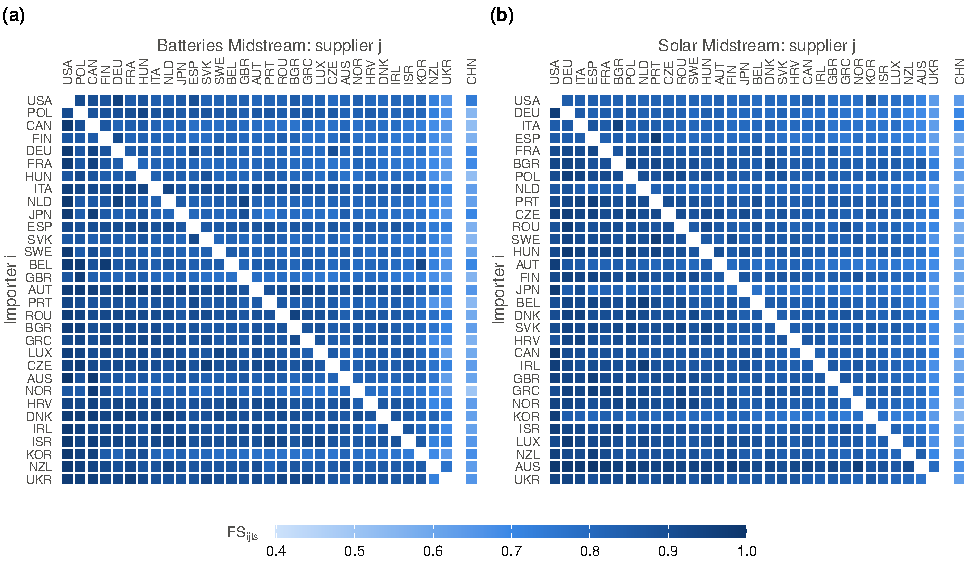
\includegraphics[width=\textwidth]{bilateral_fs_heatmap}
  \caption{Friendshore index among the core members, (a) Batteries Midstream and (b) Solar
  Midstream. Rows are importers $i$, columns suppliers $j$; colour is $\FS_{ijts}$
  (equation~\eqref{eq:fs_index}), the within-cell S-curve of the weighted mean of the components
  less the climate penalty. Rows and columns are the 31 core coalition members ordered by their mean
  rating as suppliers; the last column is China as a supplier to each core member. The diagonal is
  empty. Every dyad shown has an observed import component (importer's declaration or mirror).
  Source: \texttt{partner\_friendshore\_tbl.rds}.}
  \label{fig:bilateral_fs_heatmap}
\end{figure}

\paragraph{What makes a top supplier.} The leading suppliers of the United States (the United
Kingdom, Germany, Canada) and of Japan (the United States, Portugal, Austria) are all U.S.-leaning
except Thailand, seventh for Japan (Figure~\ref{fig:bilateral_fs_components}). Alignment is the largest
contribution to the top ten's composites (29.1 and 29.0 percent), followed by partner capability
(23.0 and 24.9), imports (18.7 and 20.1) and need (18.7 and 16.9); investment contributes 9.9 and 6.9
percent. China ranks 70th among the suppliers of the United States and 75th among those of Japan,
and would rank 10th and 8th without alignment. Because absent investment records drop out rather
than count as zero, and the summary keeps a dyad's five best cells, small aligned economies with a
few strong cells rank high: Estonia and Lithuania are the ninth and tenth suppliers of the United
States, and neither they nor the Netherlands, Ireland (both conduit centres, whose positions are
excluded) and Slovakia have an investment record in their five best cells. Scoring an absent record
at the lowest rank instead replaces all five in the United States' top ten, with Spain, Japan,
Poland, Korea and Belgium, but barely moves the headline index
(Section~\ref{subsec:robust_psi}).

\begin{figure}[tbp]
  \centering
  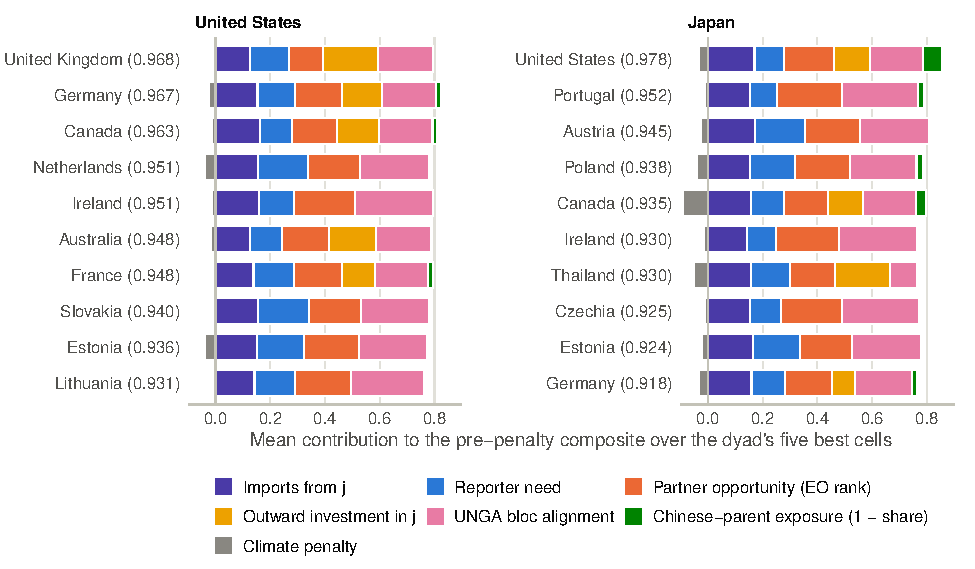
\includegraphics[width=\textwidth]{bilateral_fs_components}
  \caption{Composition of the Friendshore composite for the ten highest-ranked suppliers of the
  United States (left) and Japan (right). Each bar is the mean, over the five technology--stage
  cells behind the dyad's best-five summary $T^{\FS}_{ij}$ (in parentheses), of the weighted
  component contributions $w_c x_c/\sum_{c'\,\mathrm{obs}}w_{c'}$, which sum to the pre-penalty
  composite; the climate penalty is the negative segment. Components and weights: imports from $j$
  (2), reporter need (2), partner capability (2), outward investment in $j$ (2; IMF positions, or
  CM-FDI projects in Batteries, Electric Vehicles, Solar and Wind Midstream), UNGA bloc alignment
  (2) and Chinese-parent exposure scored as $1-$share (1, defined only in those four cells); the
  zero-weight reporter capability term is omitted. A missing segment means the component is
  unobserved for that dyad and dropped from the mean. Suppliers are ranked among partners that are
  sovereign and whose Friendshore dyad has an imputed weight share of at most 0.5 (158 for the
  United States, 170 for Japan). Source: \texttt{partner\_friendshore\_tbl.rds},
  \texttt{partner\_friendshore\_top5\_tbl.rds}; penalty recomputed from the technology emission
  index and the Climate Action Tracker ratings.}
  \label{fig:bilateral_fs_components}
\end{figure}

\paragraph{The alignment component.} Alignment carries weight 2 of 11 (18.2 percent) but 24.1
percent of the pre-penalty composite on average: for a core reporter it contributes 0.231 for a
U.S.-leaning partner, 0.115 for a nonaligned one and zero for a China-leaning one. Setting its weight
to zero changes the headline more than any other single choice examined: the Spearman correlation
with the headline $\PSI_j$ is 0.869 (0.716 for $C^{\FS}_j$), the median partner moves 17 places, and
China would rise from 44th to 3rd, India from 39th to 16th, Indonesia from 62nd to 15th and Russia
from 105th to 47th. The headline ranking is thus in large part a statement about political alignment
with the United States; a purely economic reading of supplier strength should use the variant
without it.

\paragraph{Chinese-parent exposure.} Of the 905 CM-FDI projects, 406 have a parent headquartered in
China, Hong Kong or Macao. The share is defined for 24 to 28 suppliers per covered cell, 47 economies
in all, 31 of them coalition members (Figure~\ref{fig:bilateral_cmfdi_exposure}); over the 94
supplier--technology cells outside China its median is 0.50, highest in solar (median 0.75) and
lowest in wind (0). Some partners on which the coalition relies are heavily exposed, among them
T\"urkiye, Thailand, Malaysia and Viet Nam, and in the core Korea (batteries 0.91) and Hungary
(electric vehicles 0.64). The component implements one channel, parent-company ownership, of the
common-mode upgrade proposed in the working paper on the Allied Industrial Base
\citep{neis2026allied}: plants in two supplier countries owned by
the same parent do not diversify a buyer's supply. With modest weight and narrow coverage its effect
on the headline is small (within-cell Spearman of $\FS$ with and without it 0.99; no $\PSI_j$ rank
moves by more than four places) but concentrated where it should be: the change in core members'
ratings correlates at $-0.93$ with the share, and China loses 0.085--0.095 per cell. The component
also raises the ratings of suppliers whose few foreign-invested plants have non-Chinese parents,
whoever those parents are: with it, the core's mean rating of Russia over its covered cell rises
from 0.32 to 0.40, and Argentina's from 0.42 to 0.50
(Figure~\ref{fig:bilateral_cmfdi_exposure}b). It measures the absence of Chinese ownership, not the
presence of trusted ownership. It sees
ownership of foreign-invested plants only, not dependence on Chinese equipment, precursors or
licences.

\begin{figure}[tbp]
  \centering
  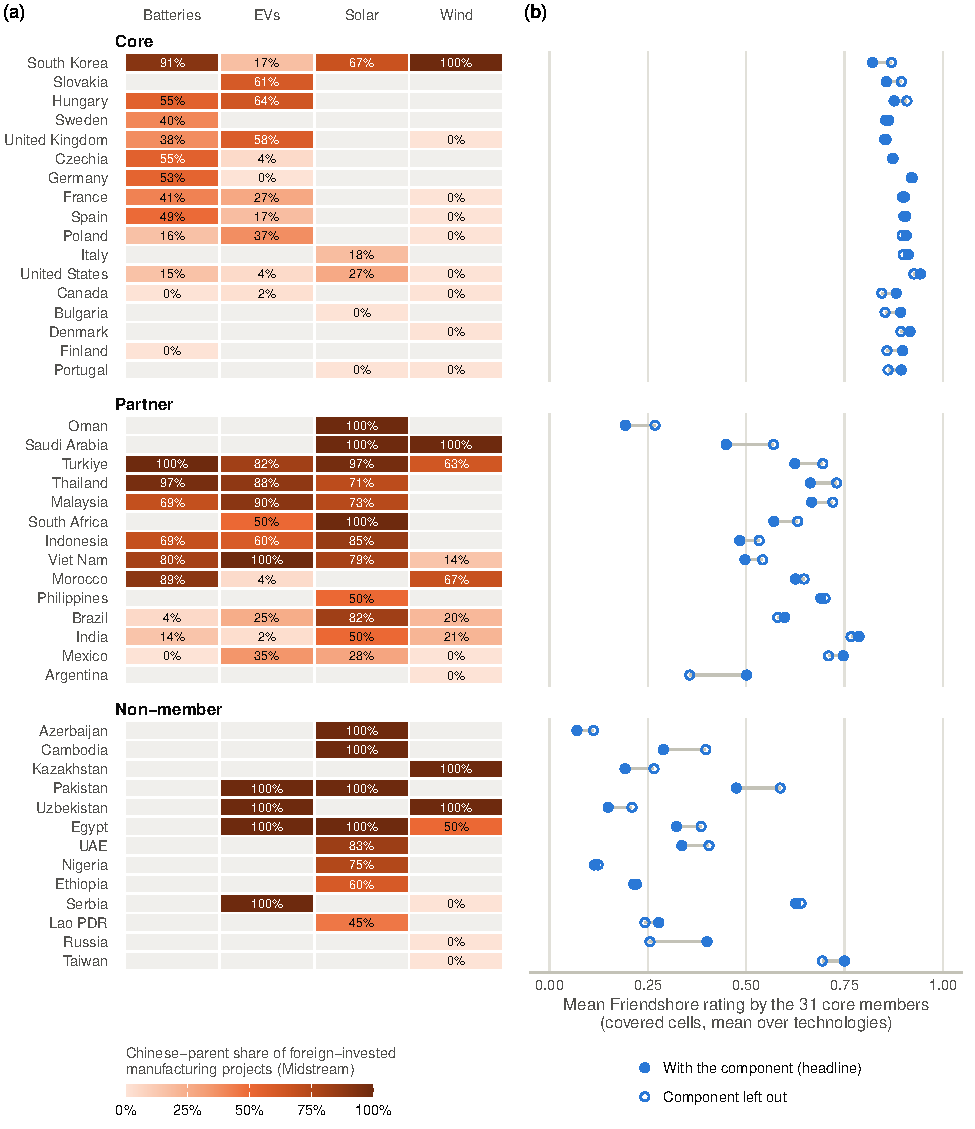
\includegraphics[width=0.93\textwidth]{bilateral_cmfdi_exposure}
  \caption{Chinese-parent ownership exposure of suppliers. Panel (a): for each economy hosting at
  least two foreign-invested manufacturing projects in a technology, the share of those projects
  owned by parents headquartered in China, Hong Kong or Macao (capital-weighted where capital is
  disclosed, by count otherwise; joint ventures attribute half to each parent), in the Midstream
  cells of batteries, electric vehicles, solar and wind; grey cells are undefined (fewer than two
  projects). Rows are grouped by coalition tier and ordered by the mean share; China, Hong Kong and
  Macao, set to one by construction, are omitted. Panel (b): the mean Friendshore rating of the
  economy by the 31 core members over its covered cells, with the component (filled) and with its
  weight set to zero and every later step re-run (open). Source: CM-FDI database, Net Zero
  Industrial Policy Lab, Johns Hopkins University (CC BY 4.0), 905 of 1,042 projects;
  \texttt{partner\_cm\_fdi\_exposure\_tbl.rds}, \texttt{partner\_friendshore\_tbl.rds}.}
  \label{fig:bilateral_cmfdi_exposure}
\end{figure}

\paragraph{The partner-level PSI.} In the headline view (Figure~\ref{fig:bilateral_psi_rank}) the
United States (0.936), Germany (0.934), the Netherlands, the United Kingdom, France, Italy, Spain,
Belgium, Poland and Czechia (0.904) rank highest. Core members hold 24 of the top 25 places (median
rank 16); the first non-member is Slovenia (25th), a member of the EU node. Partners rank lower
(median 64.5), from Saudi Arabia (38th) and India (39th) to Gabon (141st). China ranks 44th, a strong
market and a weak supplier in this view (21st on $C^{\PO}_j$, 57th on $C^{\FS}_j$), Taiwan 47th and
Switzerland 51st. Opportunity varies little across partners (standard deviation 0.031, against
0.190 for $C^{\FS}_j$ and $C^{\DP}_j$), so although nominally 40 percent of the index it accounts for
5.5 percent of the variance of $\PSI_j$ among the 130 partners with all three categories
(Friendshore 63.8, Development 30.7 percent).

\begin{figure}[tbp]
  \centering
  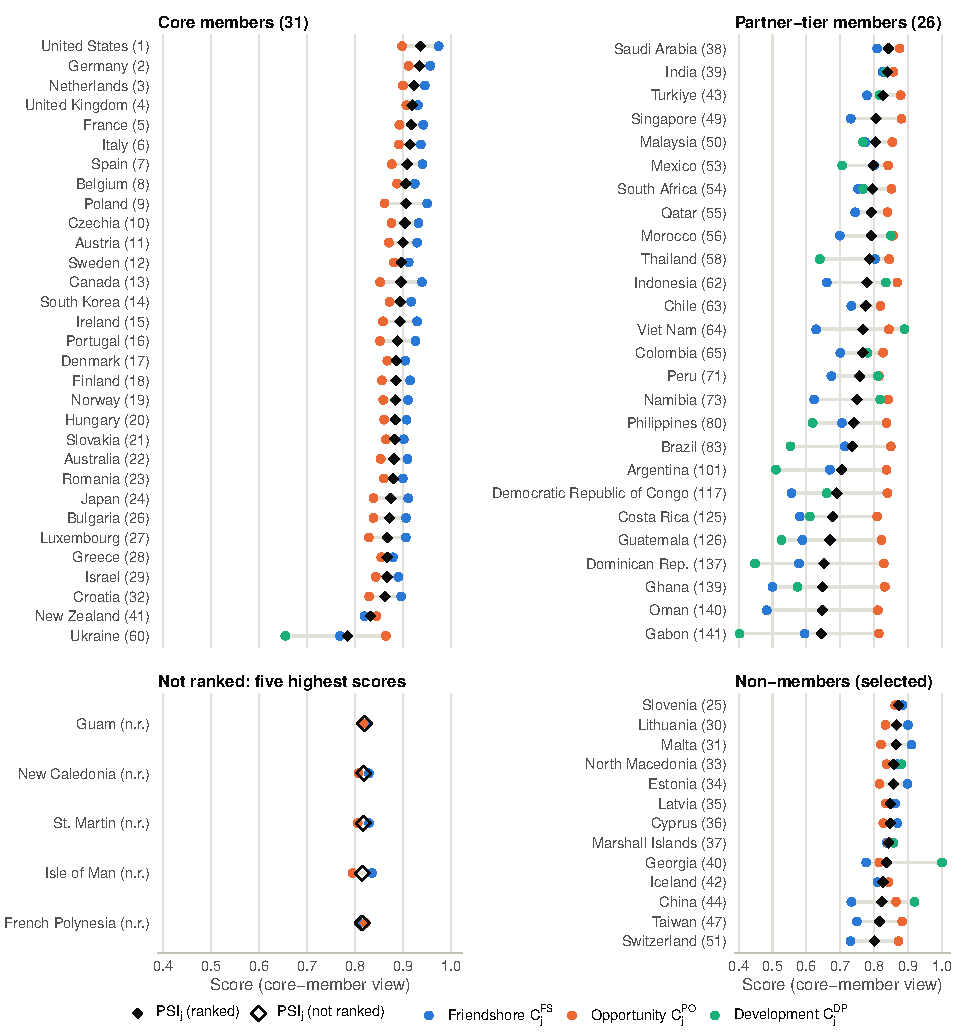
\includegraphics[width=\textwidth]{bilateral_psi_rank}
  \caption{Partnership Strength Index in the headline view. Diamonds are $\PSI_j$
  (equation~\eqref{eq:psi}) with $C^{\FS}_j$ and $C^{\PO}_j$ averaged over the 31 core coalition
  members as reporters; dots are the three category scores, Friendshore $C^{\FS}_j$, Partnership
  Opportunity $C^{\PO}_j$ and Development Potential $C^{\DP}_j$ (partners that are not high-income
  only). Panels: the 31 core members, the 26 partners, the ten highest-ranked non-members with
  China, Taiwan and Switzerland, and the five highest-scoring partners that are not ranked. Ranks
  in parentheses are among the 192 rankable partners (sovereign, imputed weight share at most 0.5);
  open diamonds and ``n.r.'' mark partners without a rank. Source: \texttt{psi\_tbl.rds}.}
  \label{fig:bilateral_psi_rank}
\end{figure}

\paragraph{Views of the index.} The core and full-coalition views agree closely (Spearman 0.981 over
192 ranked partners, median rank change 5, 13 of the top fifteen in common); the core and world views
(188 ranked) less so (0.881, median change 17, ten in common) (Table~\ref{tab:bilateral_psi_views}).
The views differ in how they place the large nonaligned and China-leaning economies: China is 44th,
9th and first in the core, full-coalition and world views, India 39th, 15th and 2nd, Indonesia 62nd,
32nd and 6th. The partners whose rating depends on who is asking are those whose alignment differs
from that of the core.

% Generated by scripts/paper/fig_bilateral.R; numbers in paper/results/bilateral.json (psi_views).
\begin{table}[t]
\centering
\begin{threeparttable}
\caption{The fifteen highest-ranked partners in the three views of the Partnership Strength Index}
\label{tab:bilateral_psi_views}
\footnotesize
\begin{tabular}{@{}r l S[table-format=1.3] l S[table-format=1.3] l S[table-format=1.3]@{}}
\toprule
 & \multicolumn{2}{c}{Core members (31 reporters)} & \multicolumn{2}{c}{Full coalition (57)} & \multicolumn{2}{c}{World (218)}\\
\cmidrule(lr){2-3}\cmidrule(lr){4-5}\cmidrule(l){6-7}
Rank & Partner & {$\PSI_j$} & Partner & {$\PSI_j$} & Partner & {$\PSI_j$}\\
\midrule
1 & United States & 0.936 & United States & 0.893 & China & 0.813\\
2 & Germany & 0.934 & Germany & 0.879 & India & 0.787\\
3 & Netherlands & 0.922 & France & 0.868 & France & 0.783\\
4 & United Kingdom & 0.919 & Netherlands & 0.864 & United States & 0.782\\
5 & France & 0.917 & Spain & 0.861 & Germany & 0.780\\
6 & Italy & 0.914 & United Kingdom & 0.857 & Indonesia & 0.768\\
7 & Spain & 0.908 & Italy & 0.854 & Netherlands & 0.764\\
8 & Belgium & 0.906 & South Korea & 0.852 & South Korea & 0.761\\
9 & Poland & 0.906 & China & 0.850 & Spain & 0.760\\
10 & Czechia & 0.904 & Belgium & 0.848 & United Kingdom & 0.757\\
11 & Austria & 0.900 & Canada & 0.847 & Italy & 0.755\\
12 & Sweden & 0.896 & Poland & 0.840 & Viet Nam & 0.753\\
13 & Canada & 0.896 & Czechia & 0.838 & Canada & 0.750\\
14 & South Korea & 0.894 & Austria & 0.838 & Austria & 0.746\\
15 & Ireland & 0.893 & India & 0.836 & Malaysia & 0.746\\
\bottomrule
\end{tabular}
\begin{tablenotes}[flushleft]\footnotesize
\item \textit{Notes:} $\PSI_j$ (equation~\eqref{eq:psi}) with $C^{\FS}_j$ and $C^{\PO}_j$ averaged over the reporters of each view: the 31 core coalition members (the headline), the 57 core and partner-tier members, and every other reporter (218 per partner). Ranks among the rankable partners of each view (sovereign, imputed weight share at most 0.5): 192, 192 and 188 partners. Spearman correlations of $\PSI_j$ across the partners ranked in both views: core and full coalition 0.981 (192), core and world 0.881 (188), full coalition and world 0.948 (188). Source: \texttt{psi\_tbl.rds}, \texttt{psi\_full\_coalition\_tbl.rds}, \texttt{psi\_world\_tbl.rds}; \texttt{scripts/paper/fig\_bilateral.R}.
\end{tablenotes}
\end{threeparttable}
\end{table}


\paragraph{Supplier and market views of the same edge.} For coalition pairs, the importer's
Friendshore rating of a supplier and the supplier's Opportunity rating of that importer as a market
agree to a degree (Figure~\ref{fig:bilateral_fs_po}; Spearman 0.715 over 95,312 matched cells),
partly through the shared capability term. Alignment, which enters only Friendshore, separates them:
Friendshore exceeds Opportunity by 0.157 on average for same-bloc pairs and falls short by 0.24 for
opposite blocs. The highest dyadic $\PSI_{ij}$ is Canada's rating of the United States (0.981).

\begin{figure}[tbp]
  \centering
  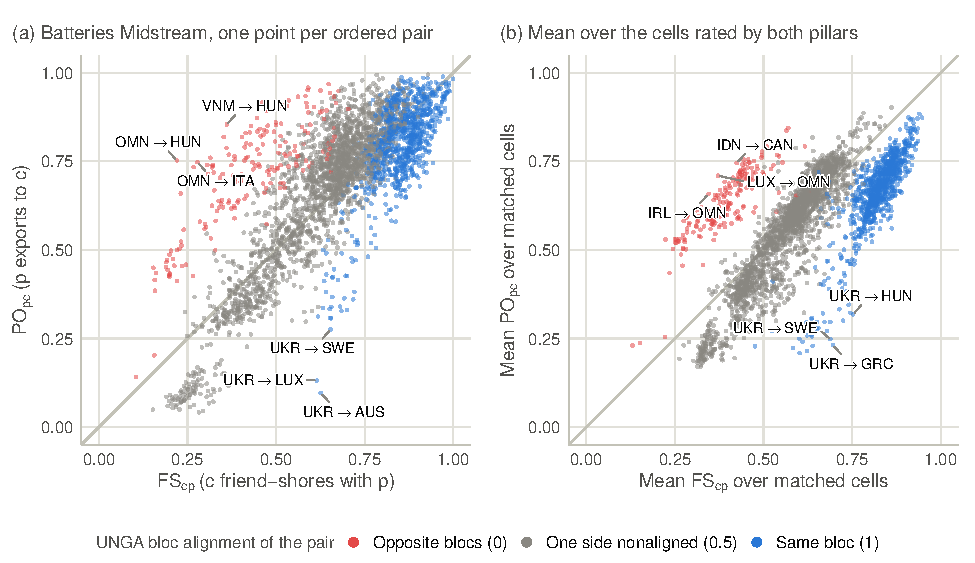
\includegraphics[width=\textwidth]{bilateral_fs_po}
  \caption{Supplier and market ratings of the same supply edge, coalition members. Horizontal:
  $\FS_{cp}$, member $c$'s Friendshore rating of member $p$ as a supplier; vertical: $\PO_{pc}$,
  $p$'s Opportunity rating of $c$ as a market. Panel (a): Batteries Midstream, one point per ordered
  pair of the 57 members (3,192 pairs). Panel (b): mean over the technology--stage cells rated by
  both pillars (28 to 30 per pair). Colour is the pair's dyadic UNGA alignment (1 same bloc, 0.5 when
  either is nonaligned, 0 opposite blocs); the line is the diagonal; the three pairs most favoured by
  each view are labelled. Source: \texttt{partner\_friendshore\_tbl.rds},
  \texttt{partner\_opportunity\_tbl.rds}.}
  \label{fig:bilateral_fs_po}
\end{figure}

\paragraph{Development potential.} Among the 125 ranked partners, Georgia, Mongolia and Mauritius
(1.00), Tuvalu and China (0.919) have the highest best-five summaries; the aid components, 35
percent of the nominal weight, provide 43.7 percent of the composite in their best cells. China's
score is a reminder that the pillar rates absorptive capacity, not alignment.

% ===========================================================================
% Section 10. Designing the Allied Industrial Base: a network optimization
% Specification: R/indices/allied_network_design.R and scripts/30_build_allied_network_design.R.
% Numbers: final full rerun of 2026-10-12, scripts/30 at lambda = 0.78 (paper/results/network.json,
% network_frontier.json). Algorithms, EU-node rules and the lambda grid: Appendix C
% (app:algorithm). Further results: Online Appendix oa:network (sections/oa_network.tex).
% Robustness of the design (fig:network_robustness, tab:network_robustness): Section 11.
% ===========================================================================
\section{Designing the Allied Industrial Base: a network optimization}
\label{sec:network}

The indices of Sections~\ref{sec:es}--\ref{sec:bilateral} score countries, sectors and pairs one at
a time. The case for an Allied Industrial Base turns on a different question
\citep{neis2026allied}: a top-ranked country may add little if its strengths duplicate the
coalition's, and a lower-ranked one may complete a resilient chain, so the object is a country's
marginal contribution to the system and the task is to optimise combinations rather than rankings.
The same source sketches a portfolio objective, security, opportunity, development and durability
gains net of cost premia, delay, duplication and residual coercion exposure, maximised under
explicit constraints such as a resilience floor and minimum diversity; because the weights are
political, it asks for a frontier of feasible choices rather than one correct weighting.

This section builds the part of that objective that the indices support. For each Upstream and
Midstream stage of the eleven headline technologies, a mixed-integer program chooses which network
nodes produce, what share each carries and which partners each supplies. It rewards fit, the
capability of producers and the quality of their partnerships, and penalises concentration through
a concave Herfindahl term, under share limits, a dual-sourcing floor and caps on the number of
stages a node may lead; the penalty weight traces a frontier between fit and dispersion, and a rule
picks one point on it. The program is a multi-sourcing variant of facility-location and network
design \citep{geoffrion1974multicommodity,owen1998strategic,melo2009facility,daskin2013network}
with dual-sourcing constraints \citep{tomlin2006value,snyder2016orms}. Its objective is a score, not
a cost, and the design is normative: it describes what a planner with these preferences would
choose, not where production will locate. Appendix~\ref{app:algorithm} states the algorithms and
Online Appendix~\ref{oa:network} reports further results.

% ---------------------------------------------------------------------------
\subsection{Nodes, stages and scores}
\label{subsec:network_sets}

The network consists of the 57 coalition members of Section~\ref{sec:coalition} (31 core members
and 26 partners) and the six EU members that belong to it only through the Union. The EU-27 is one
node, so the 63 economies form 37 nodes; its inputs are aggregated from the members with the stage
weights of Section~\ref{sec:coalition}, and edges between members are internal and dropped
(Appendix~\ref{app:algorithm}). Taiwan, Switzerland and the China-leaning suppliers outside the
coalition are not nodes. A stage is a technology with $s\in\{\text{Upstream},\text{Midstream}\}$,
22 in all; Downstream deployment serves each member's own market and is not part of the allied
division of labour. All 37 nodes enter every stage, each as a potential producer $p$ and as a
consumer $c$.

Within each stage, $\EO$ and $\ES$ are re-ranked across the nodes with the S-curve of
Section~\ref{sec:normalization}, $\tilde v_p=\Scurve(r_p)$ with $r_p=(\rank(v_p)-1)/(n_v-1)$ and
$\gamma=0.5$, so that a score measures a node's standing among its partners. The producer score is
the weighted mean of the components observed,
\begin{equation}\label{eq:net_producer_score}
  a_p=\frac{\sum_{v\in\{\EO,\ES\}}\omega_v\,\1[\tilde v_p\ \text{observed}]\,\tilde v_p}
           {\sum_{v\in\{\EO,\ES\}}\omega_v\,\1[\tilde v_p\ \text{observed}]},\qquad
  (\omega_{\EO},\,\omega_{\ES})=(0.5,\,0.2),
\end{equation}
that is, $5/7$ and $2/7$ when both are observed. Opportunity is the index closest to productive
capability; security enters as reliability, since a secure node is a steadier supplier. The Policy
index is not part of the score: its basis differs across members (IEA PAMS alone for 11 of them),
and it enters the allied picks of Section~\ref{sec:strategic} instead. In the two Geothermal stages
no node has $\ES$; in Green Hydrogen Midstream five small partners lack it.

Demand is an allocation key, not a forecast. With need $1-\widetilde{\ES}_c$ and size the S-curve of
the rank of GDP \citep{worldbank2026wdi},
\begin{equation}\label{eq:net_demand}
  \tilde d_c=
  \begin{cases}
    \tfrac12\,(1-\widetilde{\ES}_c)+\tfrac12\,\mathrm{size}_c & \text{if } \widetilde{\ES}_c \text{ is observed},\\
    \mathrm{size}_c & \text{otherwise},
  \end{cases}
  \qquad d_c=\tilde d_c\Big/\textstyle\sum_{c'}\tilde d_{c'} .
\end{equation}
Because both terms are S-curved ranks, demand is rank-compressed: the EU node, with 24.6\% of the
nodes' GDP, has a median weight of 0.035 across stages, close to the United States' 0.033, and no
node has more than 0.054 in any stage. Development potential (Section~\ref{sec:bilateral}) has zero
weight in the objective and serves only to rank build candidates (Online
Appendix~\ref{oa:network}).

% ---------------------------------------------------------------------------
\subsection{Partnership edges}
\label{subsec:network_edges}

The quality of supply from $p$ to $c$ combines the two directed partner indices of
Section~\ref{sec:bilateral}, each read from the end it describes: the consumer's friendshore rating
of the producer and the producer's opportunity rating of the consumer's market,
\begin{equation}\label{eq:net_edge}
  W_{pc}=\tfrac12\,\FS_{cpts}+\tfrac12\,\PO_{pcts},\qquad p\neq c .
\end{equation}
Friendshore carries the consumer's view of the producer as a friendshoring opportunity, where the
consumer's security need meets the producer's economic opportunity on existing trade and investment
ties, including UN-vote alignment and Chinese ownership of the producer's foreign-invested
manufacturing. A missing component counts as zero. Of the 29{,}304 stage-specific ordered pairs of distinct nodes, 90.3\% carry both
components and 9.7\% friendshore only (every pair in the two Geothermal stages and the 180 pairs
with a Green Hydrogen Midstream consumer without $\ES$); none has neither. Self-supply is valued at
the median edge of the stage,
\begin{equation}\label{eq:net_self_edge}
  W_{pp}=\operatorname{median}\{W_{qc}:\ q\neq c,\ W_{qc}\ \text{observed}\},
\end{equation}
so domestic supply competes with a typical partnership, with neither home bias nor penalty.

% ---------------------------------------------------------------------------
\subsection{The stage program}
\label{subsec:network_program}

For stage $(t,s)$ the decisions are the flows $f_{pc}\ge0$, the share of the coalition's unit
demand that $p$ supplies to $c$; the selection indicators $y_p\in\{0,1\}$; and the link indicators
$\ell_{pc}\in\{0,1\}$. Production shares are $x_p=\sum_cf_{pc}$, and the program is
\begin{subequations}\label{eq:net_milp}
\begin{align}
  \max_{f,\,y,\,\ell}\quad
    & J=\sum_{p,c} f_{pc}\,\big(w_N\,a_p+w_E\,W_{pc}\big)+w_D\sum_p\delta_p\,y_p-\lambda\sum_p x_p^2
    \label{eq:net_obj}\\
  \text{s.t.}\quad
    & \textstyle\sum_p f_{pc}=d_c && \forall c, \label{eq:net_c_demand}\\
    & \underline s\,y_p\le x_p\le\bar s\,y_p,\qquad \textstyle\sum_p y_p\ge m_P && \forall p, \label{eq:net_c_share}\\
    & \varepsilon\,d_c\,\ell_{pc}\le f_{pc}\le d_c\,\ell_{pc},\qquad \ell_{pc}\le y_p,\qquad
      \textstyle\sum_p\ell_{pc}\ge m_S && \forall p,c, \label{eq:net_c_link}\\
    & y_p=0 && \forall p\in\mathcal{X}_{ts}, \label{eq:net_c_elig}
\end{align}
\end{subequations}
with $w_N=1$, $w_E=0.5$, $w_D=0$, $\bar s=0.40$, $\underline s=0.05$, $m_P=3$, $m_S=2$,
$\varepsilon=0.10$ and $\lambda=0.78$, where $\mathcal{X}_{ts}$ holds the nodes barred by the
portfolio caps. Demand is met in full by network producers (the network is closed); no node carries
more than 40\% of a stage and a selected one at least 5\%, a stand-in for minimum efficient scale;
and every consumer has at least two suppliers, each carrying at least a tenth of its demand. These
constraints bound the Herfindahl index of designed shares, $\HHI^{\mathrm{D}}_{ts}=\sum_px_p^2$
\citep{hirschman1945national}, for any $\lambda$:
\begin{equation}\label{eq:net_hhi_bounds}
  \frac{1}{\min\{|\mathcal{E}_{ts}|,\lfloor 1/\underline s\rfloor\}}
  \ \le\ \HHI^{\mathrm{D}}_{ts}\ \le\
  \lfloor 1/\bar s\rfloor\,\bar s^{2}+\big(1-\lfloor 1/\bar s\rfloor\,\bar s\big)^{2}=0.36,
\end{equation}
where $\mathcal{E}_{ts}$ is the set of eligible producers.

The term $-\lambda\,\HHI^{\mathrm{D}}_{ts}$ is the diversification penalty, in score units per unit
of concentration. Without it the objective is linear and the solution sits at corners, two
producers at the cap and a third with the remainder. With it the marginal value of a share falls
with its size, and at an interior optimum two producers' shares differ by their difference in
marginal value divided by $2\lambda$: at $\lambda=0.78$ a score advantage of 0.0156 buys one
percentage point of share. The penalty plays the role of the variance term in portfolio choice
\citep{markowitz1952portfolio}, without a model of disruption probabilities, and it is the part of
the program that values a node by what it adds to a combination: once the leaders' marginal value
has fallen, a lower-scoring node with good partnerships enters. If supplier outages were
independent and equally likely, with probability $\pi$, the variance of the share of a stage lost
would be $\pi(1-\pi)\HHI^{\mathrm{D}}_{ts}$, so $\lambda$ reads as a price of that variance. The
penalty is additively separable, however: a producer's marginal penalty depends only on its own share,
and every node counts as an independent source, so two producers that share a bloc, a region or a
Chinese parent diversify as much as two unrelated ones. The design is therefore a first step toward
optimising combinations, not its full form (Section~\ref{sec:discussion}). The MILP carries the penalty
through tangent cuts on a share grid of 0.01, in perspective form (error at most
$2.5\times10^{-5}$ per producer; Appendix~\ref{app:algorithm}). Stages are built with
\texttt{ompr} \citep{schumacher2023ompr} and solved by GLPK \citep{makhorin2020glpk} under a
300-second limit, with a greedy water-filling heuristic as fallback.

% ---------------------------------------------------------------------------
\subsection{Portfolio caps}
\label{subsec:network_portfolio}

Solved independently, the stages would select the same strong nodes again and again,
concentrating the base in a few economies and leaving many members without a stake. The design
therefore caps the number of stages in which a node is a leading producer, rising with the
logarithm of GDP:
\begin{equation}\label{eq:net_cap}
  \kappa_i=\min\Big\{\kappa_{\max},\,\max\Big\{\kappa_{\min},\
  \operatorname{round}\Big(\kappa_{\min}+(\kappa_{\max}-\kappa_{\min})\,
  \frac{\eta_i-\min_{j}\eta_j}{\max_{j}\eta_j-\min_{j}\eta_j}\Big)\Big\}\Big\},
\end{equation}
where $\eta_i=\log(1+\mathrm{GDP}_i)$, $\kappa_{\min}=2$, $\kappa_{\max}=10$ for the largest economy, and the EU's GDP summed over its
members. A node's appearances are the stages in which it is among the five largest producers,
\begin{equation}\label{eq:net_topk}
  A_i=\big|\big\{(t,s):\ x_{i,ts}>0,\ \rho_{i,ts}\le K\big\}\big|,\qquad K=5,
\end{equation}
where $\rho_{i,ts}$ is a strict rank of the share (ties broken by producer score, then by code), so
a stage contributes at most five appearances. After all stages are solved, each node with
$A_i>\kappa_i$ is barred from the $A_i-\kappa_i$ stages in which its share times its score is
smallest, those stages are re-solved, and the count is repeated until no node exceeds its cap: a
heuristic coupling of the stages, not a joint optimum.

% ---------------------------------------------------------------------------
\subsection{Calibrating the diversification weight}
\label{subsec:network_calibration}

No price converts concentration into score, so $\lambda$ is set by a rule with an observable
anchor: the smallest value on a grid at which the median of $\HHI^{\mathrm{D}}_{ts}$ over the 22
stages is at most the median export Herfindahl index of the nodes themselves,
$\HHI^{\mathrm{N}}_{ts}$, over the 18 stages with an HS6 basket (all but Geothermal and Green
Hydrogen). $\HHI^{\mathrm{N}}_{ts}$ uses 2024 basket exports from the reconciled all-reporter
Comtrade matrix \citep{uncomtrade}, with shares within the 37 nodes and the EU counting only its
extra-EU exports. The target is 0.1556 (6.43 equivalent exporters). The design should be no more
concentrated, in the median stage, than the coalition's own exports already are; a closed network
of 37 nodes cannot match the dispersion of a world market, so world concentration would be the
wrong anchor.

The grid has 36 points (0, 0.5, every 0.01 from 0.70 to 1.00, and 1.1, 1.2 and 1.5), each a full
re-solve of the production configuration. The rule picks $\lambda=0.78$, at which the median is
0.1520, or 6.58 effective producers (Figure~\ref{fig:network_frontier}; Appendix~\ref{app:algorithm}
tabulates the grid). The pick is knife-edge. At 0.77 the median is 0.1558, missing the target by
0.0002; the median is not monotone in $\lambda$ (it rises in eight of the 35 grid steps, from
0.1485 at 0.79 to 0.1502 at 0.80, for instance), because interior shares move top-five membership
and the portfolio loop then bars different nodes; and the pick moved with every revision of the
inputs during the final data corrections. The rule, not the number, is therefore the specification,
re-applied to every full rerun. The design it selects is less fragile than the number: at
$\lambda=0.77$ and 0.79 at most 1.1\% of production moves in the mean stage
(Section~\ref{sec:robustness}). The frontier prices diversification in score, not in resource costs: at the pick the summed node
and edge terms are 5.8\% below their value at $\lambda=0$, at $\lambda=1.5$ (median index 0.095)
10.6\% below. This is the frontier of choices the conceptual objective asks for
\citep{neis2026allied}.

\begin{figure}[htbp]
  \centering
  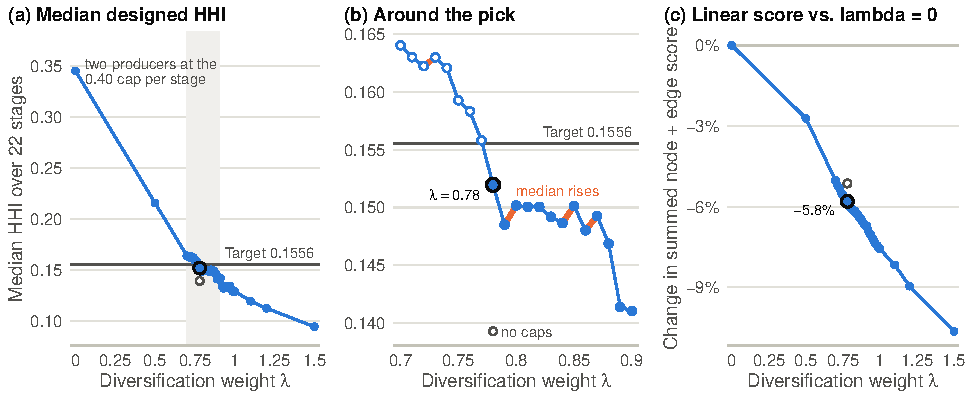
\includegraphics[width=\textwidth]{network_frontier}
  \caption{Calibration of the diversification weight $\lambda$. Panel~(a): median over the 22
  Upstream and Midstream stages of the Herfindahl index of designed production shares at each of
  the 36 grid values of $\lambda$ (37 nodes, portfolio caps on, MILP with a 300-second stage
  limit); the horizontal line is the target, the median export Herfindahl index of the nodes over
  the 18 basket stages (0.1556); the large marker is the pick, $\lambda=0.78$; the open circle the
  same design without portfolio caps. Panel~(b): the neighbourhood $0.70\le\lambda\le0.90$; open
  markers lie above the target, filled markers meet it, and orange segments are steps at which the
  median rises although $\lambda$ increases. Panel~(c): the summed node and edge terms of the 22
  stage objectives, without the Herfindahl penalty, in percent of their value at $\lambda=0$.
  Source: calibration study on the inputs of the final rerun of 12 October 2026.}
  \label{fig:network_frontier}
\end{figure}

% ---------------------------------------------------------------------------
\subsection{Results}
\label{subsec:network_results}

\paragraph{Solution.} All 22 stages are solved by the MILP, none by the fallback, and the
portfolio loop converges after seven passes; the 62 stage solves take 462 seconds, none more than
10.6.

\paragraph{Who produces what.} Figure~\ref{fig:network_specialization} and
Table~\ref{tab:network_producers} show the designed division of labour: 201 producer roles, from
seven producers (Nuclear Upstream) to ten per stage, median nine. $\HHI^{\mathrm{D}}_{ts}$ runs from
0.126 (Oil Midstream) to 0.209 (Nuclear Upstream); the largest share is 0.325 (Indonesia in Green
Hydrogen Upstream, Canada in Nuclear Upstream), none reaches the cap, and 61 sit at the floor. Twenty-nine of the 37
nodes produce somewhere; eight never do (Turkey, New Zealand, Ukraine, the Dominican Republic,
Guatemala, Ghana, Costa Rica and Gabon). Canada has the most roles (16), then the EU node (15; it leads no stage), the United States and
Indonesia (13 each). How many roles a node takes follows its size through the caps
(Spearman correlation 0.75 with the cap); which stages it takes follows its scores. Nodes outside
the high-income group carry 47\% of designed Upstream and 43\% of Midstream production.

Three patterns arise from the construction rather than from observed capacity. Indonesia,
China-leaning by its votes and a member through IPEF, leads six Upstream stages and Oil Midstream:
the producer score has no alignment term, which reaches the design only through the edges.
Thailand leads both Geothermal stages, where scores rest on $\EO$ alone and edges lack their
opportunity half. And the design applies no endowment screen: by the screen of the allied picks
(Section~\ref{sec:strategic}), 21 of the 90 designed roles in the ten screened Upstream stages are
held by nodes without recorded reserves or production of the stage's resources, a median of 11\% of
stage production (none in Electric Vehicles, Gas and Oil Upstream; 36\% in Solar Upstream). Their
shares are supply they would have to source through trade or overseas equity.

% Generated by scripts/paper/fig_network.R from data/processed/outputs/allied_network_specialization.csv
\begin{table}[htbp]
\centering
\begin{threeparttable}
\caption{Designed producers and production shares by technology and stage}
\label{tab:network_producers}
\footnotesize
\begin{tabularx}{\textwidth}{@{}>{\raggedright\arraybackslash}p{2.1cm} >{\raggedright\arraybackslash}X >{\raggedright\arraybackslash}X@{}}
\toprule
Technology & Upstream & Midstream \\
\midrule
Batteries & IDN~.23, AUS~.22, CAN~.12, CHL~.12, ARG~.08, PHL~.06, EU~.06, GBR~.05, ZAF~.05 & USA~.29, IND~.14, MYS~.14, CAN~.11, EU~.10, THA~.06, KOR~.06, GBR~.05, JPN~.05 \\
Coal & IDN~.26, IND~.15, VNM~.12, COL~.09, ZAF~.07, PER~.07, CAN~.06, THA~.06, EU~.05, PHL~.05 & JPN~.20, EU~.20, COL~.14, KOR~.12, VNM~.08, CAN~.07, ISR~.06, MEX~.05, MYS~.05 \\
Electric Grid & CHL~.31, MEX~.14, COD~.12, PER~.12, PHL~.07, AUS~.05, GBR~.05, JPN~.05, NOR~.05, ZAF~.05 & THA~.22, MEX~.15, JPN~.13, MYS~.11, EU~.10, USA~.08, CAN~.05, IDN~.05, IND~.05, MAR~.05 \\
Electric Vehicles & IDN~.24, AUS~.21, USA~.16, CHL~.08, PHL~.07, ARG~.06, EU~.05, THA~.05, ZAF~.05 & USA~.32, MEX~.20, KOR~.19, JPN~.08, VNM~.06, CAN~.05, GBR~.05, ZAF~.05 \\
Gas & USA~.25, CAN~.14, NOR~.14, QAT~.12, MYS~.10, IDN~.05, AUS~.05, IND~.05, OMN~.05, SAU~.05 & IND~.24, USA~.18, EU~.14, KOR~.12, MEX~.06, GBR~.05, IDN~.05, ISR~.05, JPN~.05, NOR~.05 \\
Geothermal & THA~.26, MYS~.15, NOR~.13, ISR~.10, EU~.08, IDN~.07, MEX~.05, CAN~.05, QAT~.05, USA~.05 & THA~.26, MYS~.15, ISR~.14, NOR~.10, QAT~.07, EU~.07, CAN~.06, IDN~.05, MEX~.05, USA~.05 \\
Green Hydrogen & IDN~.33, THA~.14, CAN~.14, EU~.12, MEX~.09, ISR~.08, GBR~.05, PHL~.05 & USA~.26, EU~.21, VNM~.14, NOR~.08, PHL~.07, SGP~.07, KOR~.06, ISR~.05, JPN~.05 \\
Nuclear & CAN~.33, NAM~.22, IND~.16, ZAF~.14, ISR~.05, SAU~.05, THA~.05 & IND~.24, EU~.20, JPN~.14, MYS~.12, ISR~.07, KOR~.06, NOR~.06, GBR~.05, MEX~.05 \\
Oil & USA~.23, SAU~.17, CAN~.17, NOR~.12, OMN~.08, QAT~.08, IDN~.05, IND~.05, THA~.05 & IDN~.20, IND~.14, KOR~.14, THA~.13, VNM~.09, JPN~.08, EU~.06, CAN~.05, MYS~.05, NOR~.05 \\
Solar & IDN~.24, CAN~.15, EU~.12, GBR~.12, NOR~.10, ZAF~.10, IND~.07, SGP~.06, MEX~.05 & IND~.28, USA~.20, VNM~.14, THA~.12, PHL~.06, CAN~.05, JPN~.05, KOR~.05, SGP~.05 \\
Wind & IDN~.22, USA~.22, AUS~.20, JPN~.08, ZAF~.06, CAN~.06, ISR~.05, KOR~.05, SGP~.05 & IND~.28, USA~.25, EU~.15, JPN~.09, MEX~.06, BRA~.06, KOR~.05, VNM~.05 \\
\bottomrule
\end{tabularx}
\begin{tablenotes}[flushleft]\footnotesize
\item \emph{Notes:} Producers of each stage in the production design (37 network nodes, diversification weight $\lambda=0.78$, portfolio caps on, every stage solved by the MILP), ordered by the designed production share $x_{p,ts}$, the share of the coalition's unit demand in the stage that the node supplies (ISO3 codes; EU = the EU-27 node; shares sum to one within a cell and are printed to two decimals). Source: \texttt{allied\_network\_specialization.csv}.
\end{tablenotes}
\end{threeparttable}
\end{table}


\begin{figure}[htbp]
  \centering
  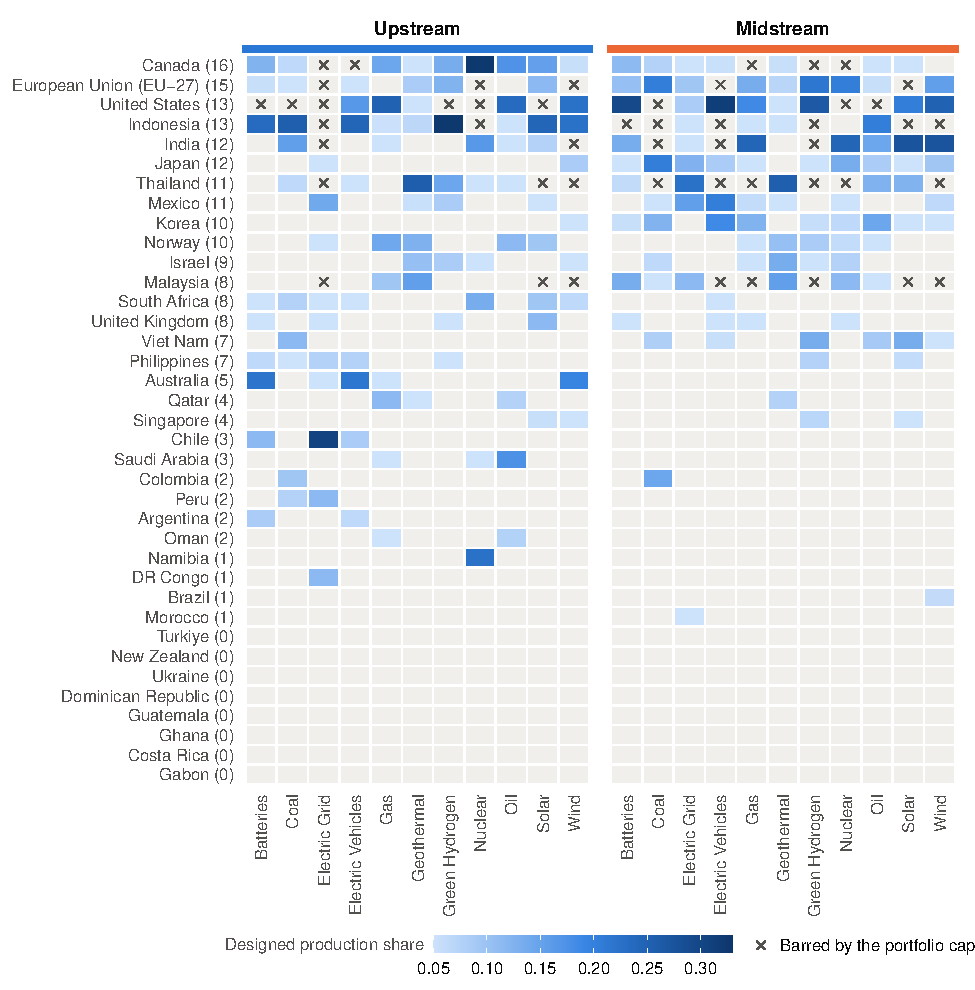
\includegraphics[width=\textwidth]{network_specialization}
  \caption{Designed division of labour across the allied network. Rows are the 37 network nodes
  (the EU-27 as one node), ordered by the number of stages in which they produce (in parentheses)
  and then by their summed share; columns are the eleven headline technologies within the
  Upstream and Midstream stages. Shading is the designed production share $x_{p,ts}$ from the
  floor 0.05 to the largest share, 0.325; light grey cells are stages in which the node does not
  produce, and a cross marks a stage from which the portfolio loop barred the node in its final
  pass. Production design: $\lambda=0.78$, GDP-log portfolio caps, node policy term off, all 22
  stages solved by the MILP. Source: \texttt{allied\_network\_specialization.csv} and
  \texttt{allied\_network\_diagnostics.csv}.}
  \label{fig:network_specialization}
\end{figure}

\paragraph{Flows.} Figure~\ref{fig:network_map} shows three Midstream stages; India leads Solar and
Wind Midstream (0.275 each) and the United States Batteries Midstream (0.295). The redundancy rules
bind: 793 of the 811 consumer--stage pairs with positive demand draw on exactly two suppliers, and
in every stage the weakest link carries exactly 10\% of its consumer's demand. With no transport cost in the objective, routing follows the edge weights: the flow-weighted edge weight is
0.874 in the median stage against an unweighted mean of 0.58, and 15 to 28\% of the mapped flows
stay within a World Bank region.

\begin{figure}[htbp]
  \centering
  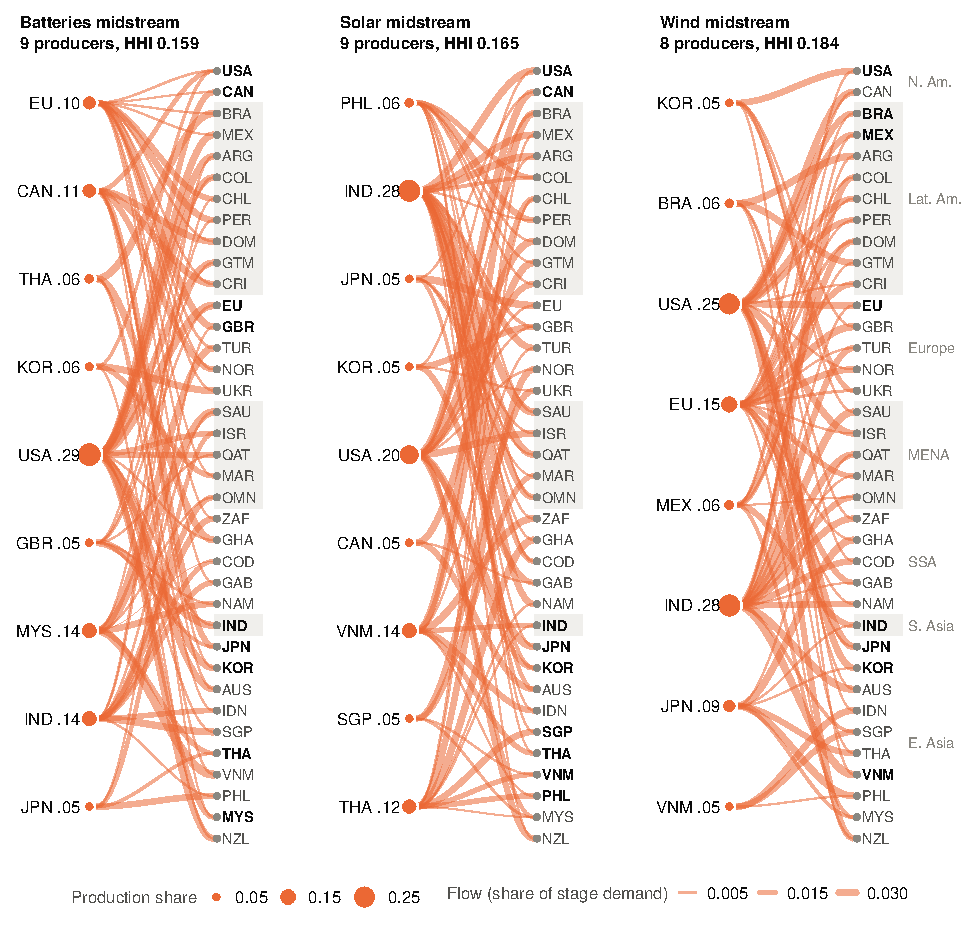
\includegraphics[width=\textwidth]{network_map}
  \caption{Designed flows in three Midstream stages. In each panel producers sit on the left,
  sized by their production share (printed next to the code; EU = the EU-27 node), and all 37
  nodes sit on the right as consumers, in the same order in every panel: by World Bank region
  (shaded bands) and by GDP within region. A line is a flow $f_{pc}$, wider for larger flows;
  consumers that also produce are in bold. Producers are placed at the flow-weighted mean position
  of their consumers (the barycentre step of a two-layer layout computed with \texttt{igraph}
  \citep{csardi2006igraph}). Panel titles give the number of producers and
  $\HHI^{\mathrm{D}}_{ts}$. Production design ($\lambda=0.78$, portfolio caps, MILP). Source:
  \texttt{allied\_network\_flows.csv} and \texttt{allied\_network\_specialization.csv}.}
  \label{fig:network_map}
\end{figure}

\paragraph{Concentration and current exporters.} Figure~\ref{fig:network_concentration} sets the
design against two benchmarks in the 18 basket stages. It meets the nodes' median export
concentration by construction, but stage by stage the two are unrelated (Spearman correlation
$-0.07$): the design spreads production where the nodes' exports are concentrated, as in Nuclear
Upstream (Canada 54\% of node exports), and concentrates it where they are dispersed. It is less
concentrated than world exports (median 0.101) in only five stages. What changes is the identity of
suppliers: China is the largest world exporter in ten basket stages (20 to 43\% of world exports),
and the 37 nodes hold 74\% of world exports in the median basket stage, so the closed design
replaces by assumption 3 to 46\% of current world supply, at a cost the model does not measure. Nor does it follow the ranking of current exporters: in the
median basket stage 66\% of designed production lies outside the three largest exporting nodes, and
designed and observed export shares have a median Spearman correlation of 0.53. Economies that do
not report to Comtrade enter these benchmarks only through their partners' mirror declarations.

\begin{figure}[htbp]
  \centering
  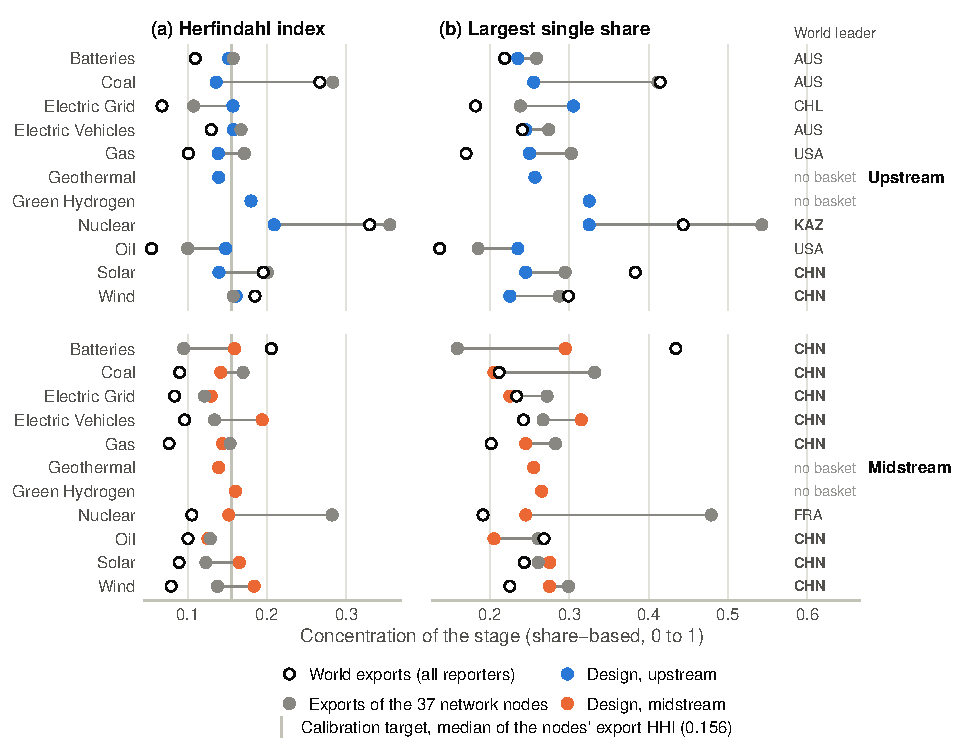
\includegraphics[width=\textwidth]{network_concentration}
  \caption{Designed versus observed concentration by technology and stage. Panel~(a): Herfindahl
  index of designed production shares, $\HHI^{\mathrm{D}}_{ts}$ (filled circles coloured by
  stage); of the 2024 basket exports of the 37 nodes, $\HHI^{\mathrm{N}}_{ts}$ (grey; the EU-27 as
  one exporter counting only extra-EU exports; reconciled Comtrade matrix, importer report else the
  exporter's mirror $\times1.06$); and of world exports across all reporters,
  $\HHI^{\mathrm{W}}_{ts}$ (open circles). The vertical line is the calibration target (0.156).
  Panel~(b): the largest single share in each case; the codes at the right name the world's
  largest exporter of the stage's basket, in bold where it is outside the network. Geothermal and
  Green Hydrogen have no basket. Production design ($\lambda=0.78$, caps on). Sources:
  \texttt{allied\_network\_diagnostics.csv}, \texttt{allied\_network\_observed\_hhi.csv}, UN
  Comtrade \citep{uncomtrade}.}
  \label{fig:network_concentration}
\end{figure}

\paragraph{Portfolio caps.} The caps range from two (Gabon, Namibia) to ten (the United States, the
EU) and sum to 218, against 110 top-five appearances; eight nodes end at their cap, and the final
pass bars 49 (node, stage) combinations in 17 stages (Figure~\ref{fig:network_portfolio}). Without
caps, the United States would be a top-five producer in 17 stages against a cap of ten. The caps
pass appearances chiefly to Japan, Mexico, the Philippines, South Africa and Israel, cost 1.9\% of
the summed objective (at most 5.9\%, in Coal Midstream) and raise the median $\HHI^{\mathrm{D}}_{ts}$
from 0.139 to 0.152, so the calibrated $\lambda$ is specific to the capped configuration.

\begin{figure}[htbp]
  \centering
  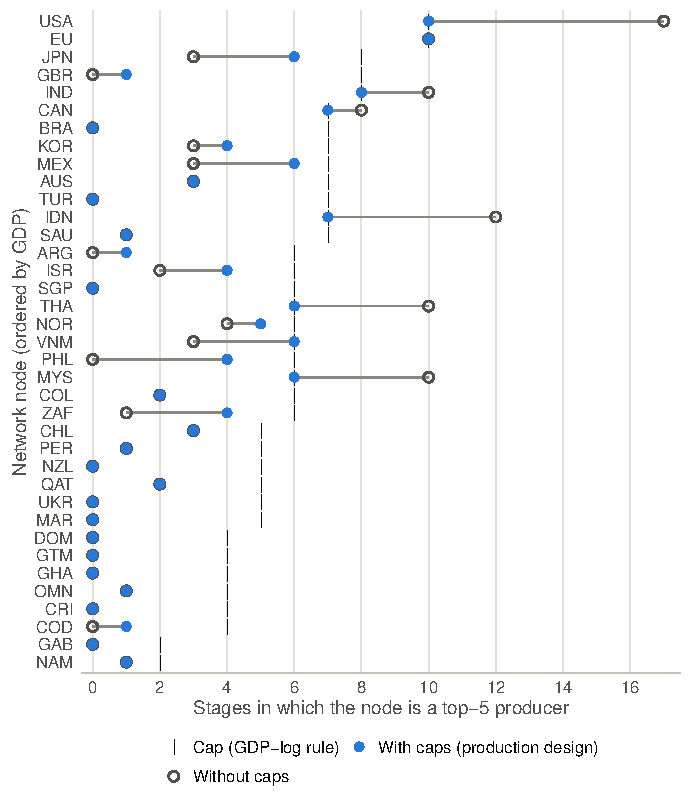
\includegraphics[width=0.75\textwidth]{network_portfolio}
  \caption{Portfolio caps and realised top-5 appearances. For each of the 37 nodes (EU = the
  EU-27 node), ordered by GDP, the vertical tick is the cap $\kappa_i$ of \eqref{eq:net_cap}, the
  filled circle the number of stages in which the node is a top-5 producer \eqref{eq:net_topk} in
  the production design, and the open circle the same count in the design solved without caps and
  otherwise unchanged ($\lambda=0.78$). GDP: latest finite WDI value in current US dollars
  \citep{worldbank2026wdi}, summed over the 27 members for the EU. Source:
  \texttt{allied\_network\_portfolio\_caps.csv}, \texttt{allied\_network\_portfolio\_counts.csv}
  and the no-caps run of the calibration study.}
  \label{fig:network_portfolio}
\end{figure}

% ---------------------------------------------------------------------------
\subsection{What the design does and does not show}
\label{subsec:network_limitations}

Against the five analytical layers of the conceptual source \citep{neis2026allied}, the design joins
the capability layer (node scores) to the complementarity layer (directed edges, with alignment and
Chinese-parent exposure) under a minimal robustness layer (share caps, dual sourcing and the
diversification penalty). It takes the severity layer as given, since all 22 stages are designed
alike, and has no bankability layer; in the source's sequence from severity to coordination to
specialization, it is the last step. Within these limits it illustrates, by construction rather than as a finding, the source's point
that an allocation under a diversification constraint need not follow the ranking of current
exporters; it does not show that the combinations are resilient, because
the program models no shocks.

Four further limits apply. The objective is a score: no unit costs, capacities, ramp-up times or
build costs enter. Stages are solved
independently, so cell manufacturing can be placed where none of the upstream supply is, although
shocks propagate along such links \citep{acemoglu2012network,carvalho2021supply}. The network is
closed: it shows how the coalition could divide its own requirement, not the cost of decoupling
\citep{aiyar2023geoeconomic,javorcik2024economic}. And exposure is direct: dyadic edges do not
register a partner's own dependence on non-members, although the economies that gained U.S. market
share from China are themselves integrated into Chinese supply chains
\citep{freund2024us,alfaro2023global}; the Chinese-parent component of friendshore captures one
channel of such common-mode exposure, ownership, but not shared precursors, equipment or logistics.

% ===========================================================================
% Section 11. Robustness and validation
% Numbers: paper/results/robustness.json (scripts/paper/fig_robustness.R) and
% paper/results/network_robustness.json (scripts/paper/fig_network_robustness.R); final rerun of
% 2026-10-12. Further detail (vintages, weight draws, curvature, imputation, rankability,
% leave-one-out and effective importance, data choices, vertical complementarities with the
% appendix sensitivity table tab:robustness_vertical): Online Appendix oa:robustness
% (sections/oa_robustness.tex).
% ===========================================================================
\section{Robustness and validation}
\label{sec:robustness}

We vary one element of the construction at a time, holding the others at the final configuration,
and ask how far the results depend on choices rather than data
\citep{saisana2005uncertainty,oecd2008handbook,saltelli2008global}. For the pillars the comparison
that matters is the ranking of countries within a technology--stage pair, so the main statistic is
the within-pair Spearman correlation with the baseline, summarised across pairs and computed over
the baseline's rankable cells: 4{,}163 of 6{,}232 scored cells in the 30 headline $\ES$ pairs and
4{,}301 of 7{,}131 in the 33 $\EO$ pairs. Every variant is recomputed from stored inputs with the
pipeline's own builders, which reproduce the published indices at the baseline settings. Online
Appendix~\ref{oa:robustness} gives the details and further tables.

% ---------------------------------------------------------------------------
\subsection{The pillars}
\label{subsec:robust_pillars}

Within-pair rankings are almost insensitive to the category weights and to the curvature of the
S-curve (Figure~\ref{fig:robustness_variants}). Over 1{,}000 Dirichlet draws centred on the
configured weights (coefficient of variation 0.3 for a category of average weight), the median
within-pair correlation is 0.997 in $\ES$ and 0.988 in $\EO$, and equal weights give 1.000.
Re-curving every component to $\gamma=0.25$, 1 (the plain percent rank) or 2 gives medians between
0.964 and 0.997 in $\ES$ and between 0.965 and 0.992 in $\EO$, the lowest at $\gamma=2$. Much of
this stability is mechanical: all scored countries of a pair observe the same categories, so a
category that is constant within the pair shifts every country alike
(equation~\eqref{eq:affine_constant}), and the median pair has only three varying categories in
$\ES$ and four in $\EO$. A high average can also hide wide rank bands for individual members
(Online Appendix~\ref{oa:robustness}).

The imputation rule matters more. Without the global-average imputation $\ES$ is unchanged in the
median pair (1.00) and $\EO$ nearly so (0.97), but the pooled $\EO$ correlation is 0.85 and the
minimum 0.29; filling gaps with zeros lowers the $\EO$ median to 0.77. Outside the economies that the
narrow sources cover, $\EO$ rankings depend on how gaps are filled, which is why the rankability rule
withholds cells whose index rests mostly on imputed components. Its threshold is itself
consequential: at $\tau=0.3$ the Strategic Index shrinks from 3{,}154 cells for 174 countries to
1{,}577 cells for 107, and at $\tau=0.7$ it grows to 5{,}156 cells for 194. The 2020 and 2025
vintages, which re-derive only the time-varying sources (about a third of the average cell's
weight), give median within-pair correlations of 0.99 in $\ES$ and 0.87 in $\EO$. Leaving out one
category confirms that nominal weights and effective importance diverge
\citep{paruolo2013ratings,becker2017weights}: Technology Demand, the largest nominal $\EO$ weight,
barely moves the median ranking, while Foreign Dependency, Cost Competitiveness and Trade carry most
of it.

\begin{figure}[tbp]
  \centering
  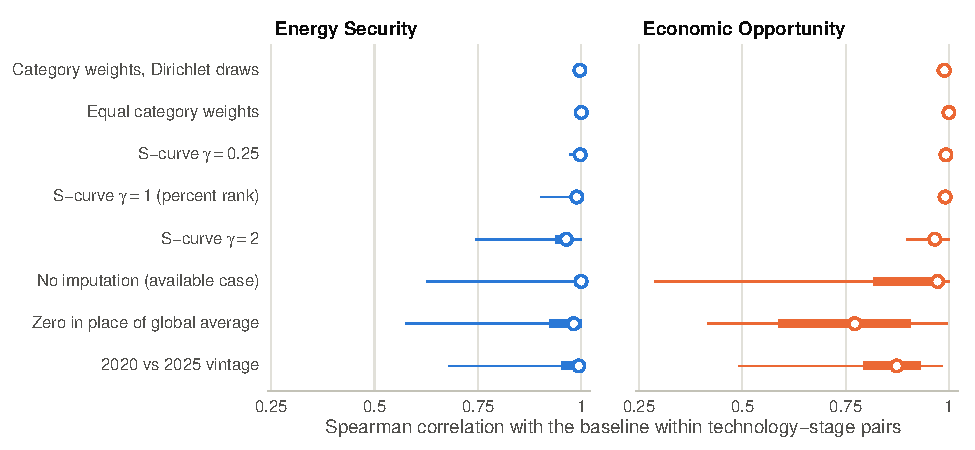
\includegraphics[width=\textwidth]{robustness_variants}
  \caption{Stability of within-pair country rankings under alternative constructions of the
  pillars. Each row is one variant; for each technology--stage pair the Spearman rank correlation
  across countries between the baseline pillar and the variant is computed over the baseline's
  rankable cells, and the row summarises these correlations across pairs: open circle, median;
  thick bar, interquartile range; thin line, minimum to maximum. For the Dirichlet weight draws the
  per-pair value is the median over 1{,}000 draws. The S-curve rows rebuild both pillars from the
  theme tables with every component re-curved to $\gamma=0.25$, 1 or 2 (baseline 0.5). ``No
  imputation'' removes every global-average rule, so uncovered countries drop the component;
  ``Zero'' fills them with 0. The last row compares the 2020 and 2025 vintages. Sample: 30 $\ES$
  pairs (4{,}163 rankable cells) and 33 $\EO$ pairs (4{,}301). Source: \texttt{index\_outputs.rds},
  theme tables and vintages of the final run; \texttt{scripts/paper/fig\_robustness.R}.}
  \label{fig:robustness_variants}
\end{figure}

% ---------------------------------------------------------------------------
\subsection{The Strategic Index and the allied picks}
\label{subsec:robust_si}

The ordering of a country's sectors is robust; its single top sector is not. Under 1{,}000 Dirichlet
draws of the five weights of equation~\eqref{eq:si}, the median within-country Spearman correlation
is 0.96 (0.88 to 0.99), but a member keeps its allied pick in 73 per cent of the draws on average,
16 of the 57 members in at least 90 per cent and 10 in fewer than half
(Figure~\ref{fig:robustness_si}). Retention follows the pick's margin over the runner-up (Spearman
correlation 0.84), and the margins are small: a median of 0.015, below 0.005 for 10 members and
below 0.01 for 21, smallest for Luxembourg (0.0005) and Indonesia (0.0007). Electric Grid and Nuclear
Midstream picks rest on the finest margins (medians 0.003 and 0.007, against 0.014 for Batteries
Midstream). The Nuclear Midstream picks of Costa Rica, the Dominican Republic, Guatemala and Namibia
have wide margins for a reason other than capability, and not because of a floor in the security
pillar: each may pick among only four sectors, the Midstream stages of nuclear, oil, gas and coal
(Namibia also Nuclear Upstream), Midstream nuclear security is compressed around its median, and the
technology greenhouse-gas weight favours nuclear (0.999, against 0.42 for gas, 0.02 for coal and 0
for oil); without the sector priors the Dominican Republic, Guatemala and Namibia move to Oil
Midstream.

Table~\ref{tab:robustness_picks} reports discrete variants. Reading security as strength rather
than need is the most consequential: the pooled Spearman correlation with the baseline is 0.33 and
only 5 of the 57 picks survive. Without the sector priors 31 picks survive, with all terms ranked
within country 20, without the policy term 30 and with equal weights 39. Switching the endowment
screen off changes 41 picks, raising Upstream picks from 14 to 47: a country without uranium scores
zero on the reserve and production terms, sits near the floor of the security pillar (86 of 174
countries share one $\ES$ value in Nuclear Upstream) and so shows a high need. The screen is a rule
of eligibility, not part of the index, and without it the Upstream picks would largely reflect that
floor. Tightening the screen to require recorded production, rather than any recorded
reserves, removes all eight Nuclear Upstream picks, whose holders have small identified resources
and no mine production, and the two Wind Upstream picks: nine members change pick and Gabon is left
without an eligible sector. Two variants address the implicit sector priors of
Section~\ref{subsec:si_definition}. Removing the cell-constant inputs from the pillar levels keeps
the within-member ordering (median Spearman correlation 0.95) but only 29 of the 57 picks, and 23 picks
then fall on Electric Grid Midstream; entering opportunity and need as within-pair ranks keeps 27
picks (median within-member correlation 0.80). The basis of the Policy index matters for its values more than for the picks: for the 65
countries with both components, the within-country correlation between policy on IEA PAMS alone and
on the composite has a median of 0.48 (interquartile range 0.41 to 0.57), yet IEA PAMS alone keeps
45 picks, and requiring both components keeps the 46 CAT-rated members' picks exactly while removing
the 11 scored on IEA PAMS alone. Adding back the October 2026 NIPO component (77 jurisdictions)
keeps only 34 picks, shifting them from Batteries Midstream (27 to 15) towards Nuclear Upstream (8 to
14).

The picks also rest on the trade data. Setting the EIA-filled fossil production to zero changes no
pick and removing the new Upstream trade baskets changes four, but dropping the Trade category keeps
29 of the 54 members that still have a pick, Trade on the Atlas basis 49, and the 2025 and 2020
vintages 48 and 44. The recorded history agrees: before the energy-trade file was completed,
Electric Grid Midstream was the pick of 17 and Batteries Midstream of 11 of the 45 members then with
a pick, against 4 and 27 of 57 in the final build. The allied pick is an informative but fragile summary, stable to the fill rules and
basket additions of the final revision and sensitive to how trade is measured.

\begin{figure}[tbp]
  \centering
  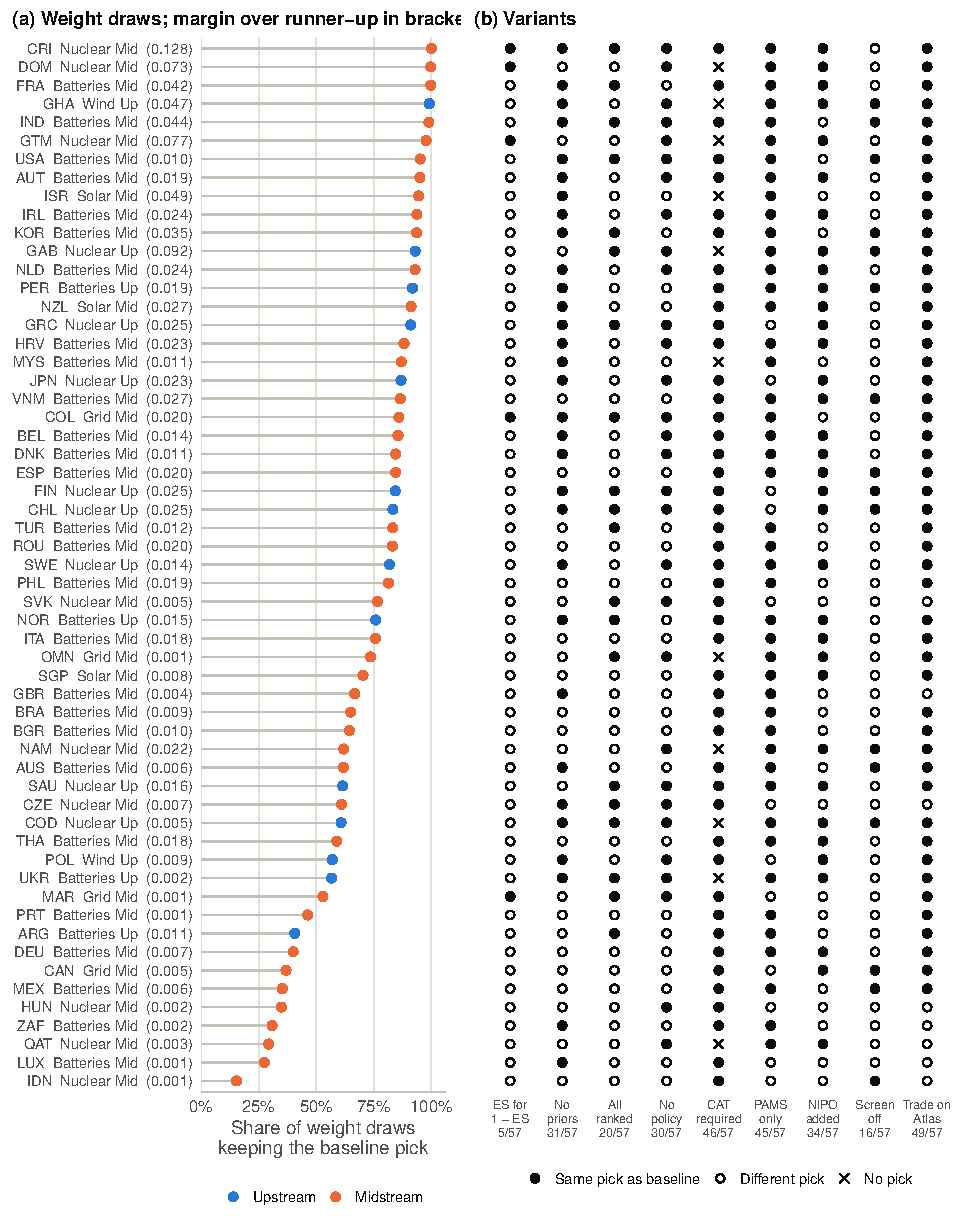
\includegraphics[width=\textwidth,height=0.70\textheight,keepaspectratio]{robustness_si}
  \caption{Robustness of the allied picks. Each row is a coalition member, its baseline pick (the
  eligible Upstream or Midstream sector with the highest Strategic Index) and, in brackets, the
  margin over its second eligible sector. Panel~(a): share of 1{,}000 Dirichlet draws of the five
  Strategic Index weights, centred on $(0.2,0.3,0.3,0.1,0.1)$ with concentration 43.4, under which
  the pick is unchanged; colour gives the stage of the pick. Panel~(b): filled circle, pick
  unchanged under the variant; open circle, changed; cross, no pick. Variants: security in place of
  need; no stage and technology priors; $\EO$ and $1-\ES$ S-curved within country; no policy term;
  both Policy components required; IEA PAMS only; the October 2026 NIPO component added back; the
  endowment screen off; Trade on the Atlas basis. Sample: 3{,}154 Strategic Index cells of 174
  countries; 57 members, all with a baseline pick. Source: \texttt{index\_outputs.rds},
  \texttt{policy\_component\_tbl}, the October 2026 NIPO component;
  \texttt{scripts/paper/fig\_robustness.R}.}
  \label{fig:robustness_si}
\end{figure}

% Generated by scripts/paper/fig_robustness.R; do not edit by hand.
\begin{table}[tbp]
  \centering
  \begin{threeparttable}
  \caption{Allied picks by sector under the baseline and the variants of the Strategic Index}
  \label{tab:robustness_picks}
  \footnotesize
  \setlength{\tabcolsep}{4pt}
  \begin{tabular}{lrrrrrrrrr}
    \toprule
    \multicolumn{10}{l}{\emph{Panel A. Specification and Policy index}}\\
    Sector & \makecell{Base-\\line} & \makecell{$\ES$ for\\$1-\ES$} & \makecell{No\\priors} & \makecell{All\\ranked} & \makecell{No\\policy} & \makecell{Equal\\weights} & \makecell{CAT\\required} & \makecell{PAMS\\only} & \makecell{NIPO\\added} \\
    \midrule
    Nuclear Upstream & 8 & 2 & 14 & 13 & 20 & 1 & 6 & 4 & 14 \\
    Batteries Upstream & 4 & 1 & 3 & 4 & 2 & 2 & 3 & 4 & 6 \\
    Wind Upstream & 2 & 0 & 2 & 0 & 3 & 1 & 1 & 1 & 3 \\
    Coal Upstream & 0 & 0 & 1 & 0 & 0 & 0 & 0 & 0 & 0 \\
    Electric Grid Upstream & 0 & 3 & 1 & 1 & 1 & 0 & 0 & 0 & 0 \\
    Electric Vehicles Upstream & 0 & 0 & 1 & 0 & 0 & 0 & 0 & 0 & 0 \\
    Gas Upstream & 0 & 1 & 0 & 0 & 0 & 0 & 0 & 0 & 0 \\
    Oil Upstream & 0 & 2 & 3 & 0 & 0 & 0 & 0 & 0 & 0 \\
    Solar Upstream & 0 & 0 & 2 & 4 & 1 & 0 & 0 & 0 & 2 \\
    Batteries Midstream & 27 & 0 & 15 & 5 & 8 & 30 & 26 & 34 & 15 \\
    Nuclear Midstream & 9 & 28 & 2 & 8 & 9 & 8 & 5 & 5 & 7 \\
    Electric Grid Midstream & 4 & 7 & 1 & 15 & 13 & 4 & 3 & 3 & 5 \\
    Solar Midstream & 3 & 2 & 2 & 1 & 0 & 9 & 2 & 6 & 4 \\
    Electric Vehicles Midstream & 0 & 0 & 0 & 0 & 0 & 0 & 0 & 0 & 1 \\
    Gas Midstream & 0 & 10 & 0 & 0 & 0 & 0 & 0 & 0 & 0 \\
    Oil Midstream & 0 & 1 & 10 & 6 & 0 & 0 & 0 & 0 & 0 \\
    Wind Midstream & 0 & 0 & 0 & 0 & 0 & 2 & 0 & 0 & 0 \\
    \midrule
    Members with a pick & 57 & 57 & 57 & 57 & 57 & 57 & 46 & 57 & 57 \\
    Same pick as baseline & 57 & 5 & 31 & 20 & 30 & 39 & 46 & 45 & 34 \\
    \addlinespace
    \midrule
    \multicolumn{10}{l}{\emph{Panel B. Data: endowment screen, final data choices, trade and reserves inputs, vintage}}\\
    Sector & \makecell{Base-\\line} & \makecell{Screen\\off} & \makecell{Zero for\\EIA} & \makecell{No new\\baskets} & \makecell{Trade on\\Atlas} & \makecell{No\\Trade} & \makecell{No\\Reserves} & \makecell{2025\\vintage} & \makecell{2020\\vintage} \\
    \midrule
    Nuclear Upstream & 8 & 17 & 8 & 11 & 8 & 9 & 14 & 9 & 8 \\
    Batteries Upstream & 4 & 12 & 4 & 4 & 4 & 1 & 1 & 4 & 5 \\
    Wind Upstream & 2 & 5 & 2 & 1 & 2 & 1 & 2 & 2 & 1 \\
    Electric Grid Upstream & 0 & 1 & 0 & 0 & 0 & 0 & 0 & 0 & 0 \\
    Solar Upstream & 0 & 12 & 0 & 0 & 0 & 0 & 0 & 0 & 0 \\
    Batteries Midstream & 27 & 7 & 27 & 25 & 26 & 13 & 24 & 25 & 23 \\
    Nuclear Midstream & 9 & 2 & 9 & 9 & 4 & 0 & 8 & 4 & 4 \\
    Electric Grid Midstream & 4 & 1 & 4 & 4 & 5 & 10 & 4 & 5 & 11 \\
    Solar Midstream & 3 & 0 & 3 & 3 & 7 & 19 & 4 & 7 & 5 \\
    Electric Vehicles Midstream & 0 & 0 & 0 & 0 & 0 & 1 & 0 & 0 & 0 \\
    Gas Midstream & 0 & 0 & 0 & 0 & 1 & 0 & 0 & 1 & 0 \\
    \midrule
    Members with a pick & 57 & 57 & 57 & 57 & 57 & 54 & 57 & 57 & 57 \\
    Same pick as baseline & 57 & 16 & 57 & 53 & 49 & 29 & 50 & 48 & 44 \\
    \bottomrule
  \end{tabular}
  \begin{tablenotes}[flushleft]\scriptsize
    \item \emph{Notes:} Number of coalition members whose allied pick, the Upstream or Midstream sector (excluding Geothermal and Green Hydrogen, and Upstream cells without a recorded resource base) with the highest Strategic Index, falls in each sector. All 57 members have a pick in the baseline. Panel A: $\ES$ for $1-\ES$, security in place of need; No priors, without the stage and technology terms; All ranked, $\EO$ and $1-\ES$ S-curved within country; No policy, without the policy term; Equal weights, 0.2 on each term; CAT required, both Policy components required (\texttt{OPSI\_POLICY\_REQUIRE\_ALL=1}), which leaves 65 countries with a Policy index and 46 members with a pick; PAMS only, CAT dropped for every country; NIPO added, the October 2026 NIPO component (GTA NIPO as of 5 October 2026) re-enters the Policy index with weight 4 (IEA PAMS 3, CAT 2), IEA PAMS still required, for its 77 policy-eligible jurisdictions. Panel B: Screen off, every Upstream cell eligible, including the 669 of 998 scored Upstream cells without recorded reserves or production; Zero for EIA, the oil, gas and coal production that the Energy Institute does not report set to zero instead of the EIA value (the rule until 11 October 2026); No new baskets, the Trade category removed from Electric Vehicles, Wind, Nuclear and Solar Upstream, whose trade baskets were added on 11 October 2026; Trade on Atlas, the Trade category of both pillars replaced by its Atlas-based counterpart of the 2025 vintage; No Trade, No Reserves, the category dropped from the pillars that score it and the remaining categories renormalised; 2025 and 2020 vintage, both pillars taken from the vintage builds, in which only the time-varying sources differ. The Policy index is the headline one in Panel B. Source: \texttt{index\_outputs.rds}, \texttt{data/processed/vintages}; \texttt{scripts/paper/fig\_robustness.R}.
  \end{tablenotes}
  \end{threeparttable}
\end{table}


% ---------------------------------------------------------------------------
\subsection{Vertical complementarities}
\label{subsec:robust_vertical}

The pillars score each stage separately, although shocks propagate along input--output links
\citep{acemoglu2012network,carvalho2021supply} and capabilities in one activity ease entry into
related ones \citep{hidalgo2007product}. A companion study tested whether a stage's $\EO$ should
reward capability in the adjacent stage and its $\ES$ the security of its inputs. On the Atlas panel
of 172 economies (1995--2023), with country--year and technology--year fixed effects, adjacent-stage
capability is associated with a stage's market-share growth and entry into comparative advantage
\citep{balassa1965trade} across countries, but the association is concentrated in fossil fuels and
nuclear, close to zero for the clean-technology chains, zero within country--technology cells, and
of no help out of sample. A sourcing-weighted input-security measure reflects mostly alignment, its
post-2022 shift is driven by Russia, and it did not predict the import shortfalls of 2021--22, whereas
the concentration of sourcing did. At the weights the evidence supports, an adjacent-stage $\EO$
term moves one pick and an input-security $\ES$ term moves ten, no more than a placebo with permuted
scores (Online Appendix~\ref{oa:robustness}). We therefore keep the stages uncoupled and leave to
future work plant-level co-location from the CM-FDI and BNEF project data, input shares weighted by
input--output coefficients, a test of sourcing concentration on the 2023 export controls on graphite
and gallium, and a co-location term in the network design.

% ---------------------------------------------------------------------------
\subsection{The partnership index}
\label{subsec:robust_psi}

The headline PSI averages the dyadic index over the 31 core members' viewpoints. The full-coalition
view (57 reporters) gives nearly the same ranking (Spearman correlation 0.98 over 192 partners, 13 of
the top 15 in common), although China moves from 44th to 9th; the world view (218 reporters) differs
more (0.88, 10 of the top 15, median absolute rank change 17). The viewpoint is a choice of whose
interests the index represents (Figure~\ref{fig:robustness_psi_views}). Without the CM-FDI parts of
friendshore, in the integration study on the inputs of 11 October 2026, the core PSI is practically
unchanged (Spearman correlation 0.9998, largest rank change five places, same top 15).

Two further sensitivities concern Friendshore. Scoring an absent outward-investment record at the
lowest rank rather than dropping it from the available-case mean leaves the core PSI almost
unchanged (Spearman correlation 0.994, 14 of the top 15 in common, largest rank change 34 places,
China from 44th to 37th), although it reorders the top suppliers of individual reporters
(Section~\ref{sec:bilateral}). The discretisation of alignment matters more. With continuous
alignment, $p_i=s_i$ so that $A_{ij}=s_is_j+(1-s_i)(1-s_j)$, the Spearman correlation with the
headline is 0.904, 12 of the top 15 are shared, the median partner moves 13.5 places and China
rises from 44th to 9th; with tercile blocs (cuts at $s=0.164$ and 0.305, 65 economies in each outer
bloc) the correlation is 0.952, 14 of the top 15 are shared and China ranks 40th. The quartile
cuts thus hold China down mainly through the step from a continuous to a three-valued alignment,
less through where the cuts fall.

\begin{figure}[tbp]
  \centering
  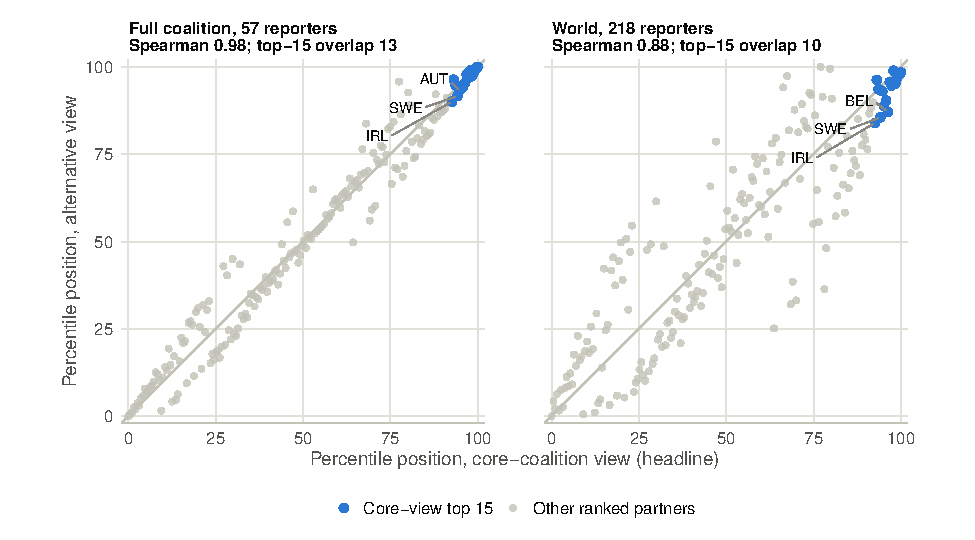
\includegraphics[width=\textwidth]{robustness_psi_views}
  \caption{The partnership index from three viewpoints. Each point is a partner ranked in both
  views ($\tau=0.5$), placed by its percentile position in the core-coalition view, the headline
  average over the 31 core members' ratings (horizontal), and in an alternative view (vertical):
  left, the full coalition of 57 reporters; right, the world of 218 reporters. Blue marks the top 15
  of the core view; the labelled points are the three of them with the lowest position in the
  alternative view. Panel titles give the Spearman correlation with the core view and the overlap of
  the top 15. Source: \texttt{psi\_tbl.rds}, \texttt{psi\_full\_coalition\_tbl.rds},
  \texttt{psi\_world\_tbl.rds}; \texttt{scripts/paper/fig\_robustness.R}.}
  \label{fig:robustness_psi_views}
\end{figure}

% ---------------------------------------------------------------------------
\subsection{The network design}
\label{subsec:robust_network}

Figure~\ref{fig:network_robustness} and Table~\ref{tab:network_robustness} re-solve the design of
Section~\ref{sec:network} with one setting changed, on inputs assembled as in production (the re-run
of the production configuration reproduces it to $5\times10^{-16}$). Each variant is compared with
the production design stage by stage through the Jaccard overlap of the producer sets and the share
of production reassigned, $\tfrac12\sum_p|x^{\mathrm{alt}}_{p,ts}-x_{p,ts}|$. The neighbouring values
of $\lambda$ leave the design almost unchanged: at 0.77, 21 of the 22 producer sets are identical
and 0.5 per cent of production is reassigned in the mean stage; at 0.79, 19 and 1.1 per cent. The
calibration is knife-edge in its number, not in what it selects. Demand matters little, since it
enters the choice of producers only through the edges and redundancy constraints and is
rank-compressed (size only: 3.4 per cent reassigned). The edge weight matters more ($w_E=0$ and 1
reassign 8.4 and 10.8 per cent), and the portfolio caps most: without them 18.5 per cent of
production is reassigned in the mean stage, 46.5 per cent in Electric Grid Upstream. Solved greedily
with the caps, the design is more concentrated (median index 0.160, above the calibration target) and
scores 2.5 per cent lower. These tests concern the stability of the design to its specification, not
its robustness to shocks, which the program does not model beyond the redundancy floor.

\begin{figure}[tbp]
  \centering
  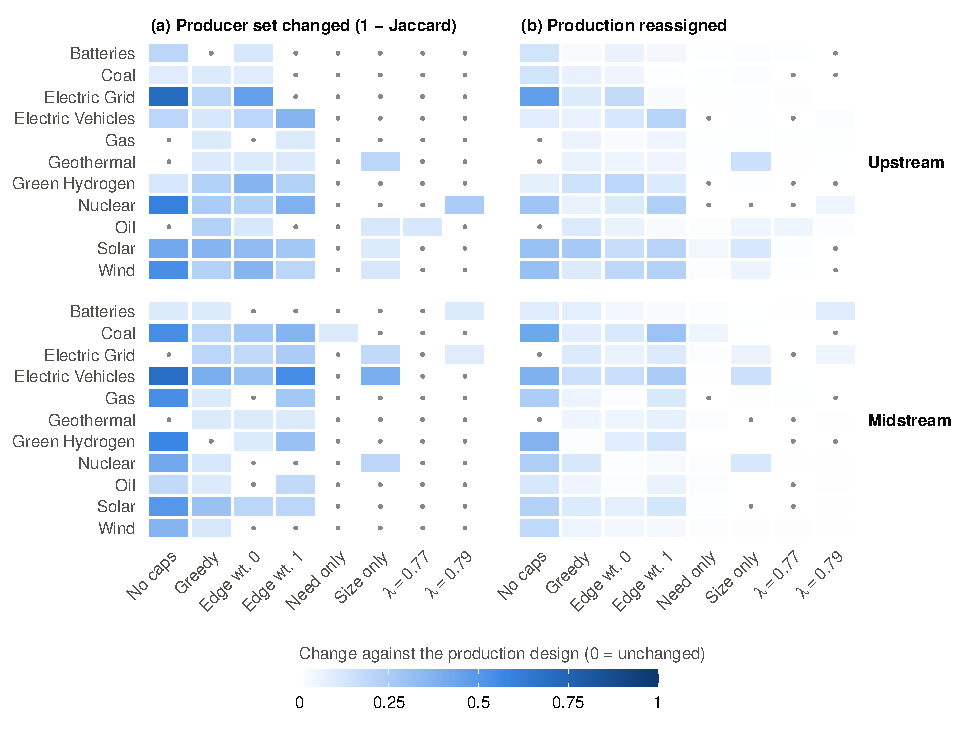
\includegraphics[width=\textwidth]{network_robustness}
  \caption{Robustness of the network design, by stage and variant. Each column re-solves the 22
  Upstream and Midstream stage programs on the 37 nodes with one setting changed: no portfolio
  caps; the greedy heuristic instead of the MILP (caps on); edge weight $w_E=0$ or 1 instead of
  0.5; demand from need only or size only; and $\lambda=0.77$ or 0.79 instead of 0.78.
  Panel~(a): one minus the Jaccard overlap $|A\cap B|/|A\cup B|$ of the stage's producer sets in the
  variant and the production design. Panel~(b): share of the stage's production assigned to
  different nodes, $\tfrac12\sum_p|x^{\mathrm{alt}}_{p,ts}-x_{p,ts}|$. Both are 0 when the stage is
  unchanged (dot) and 1 when the producer sets are disjoint. Source:
  \texttt{scripts/paper/fig\_network\_robustness.R}, on the inputs of the final rerun of 12 October
  2026.}
  \label{fig:network_robustness}
\end{figure}

% Generated by scripts/paper/fig_network_robustness.R
\begin{table}[htbp]
\centering
\begin{threeparttable}
\caption{Robustness of the network design to one setting at a time}
\label{tab:network_robustness}
\footnotesize
\begin{tabular}{@{}l r r r r r r r r@{}}
\toprule
 & \multicolumn{4}{c}{Against the production design} & \multicolumn{4}{c}{Design of the variant} \\
\cmidrule(lr){2-5}\cmidrule(l){6-9}
Variant & Jaccard & Min. & \makecell[r]{Identical\\stages} & \makecell[r]{Re-\\assigned} & \makecell[r]{Median\\$\HHI^{\mathrm{D}}$} & \makecell[r]{Pro-\\ducers} & \makecell[r]{Max.\\share} & \makecell[r]{MILP\\stages} \\
\midrule
Production design & -- & -- & -- & -- & 0.152 & 9 & 0.325 & 22 \\
\addlinespace
No portfolio caps & 0.692 & 0.294 & 5 & 0.185 & 0.139 &   10 & 0.312 & 22 \\
Greedy heuristic & 0.836 & 0.600 & 2 & 0.086 & 0.160 &    9 & 0.346 & 0 \\
Edge weight $w_E=0$ & 0.840 & 0.538 & 6 & 0.084 & 0.146 &    9 & 0.295 & 22 \\
Edge weight $w_E=1$ & 0.825 & 0.455 & 7 & 0.108 & 0.157 &    9 & 0.355 & 22 \\
Demand from need only & 0.995 & 0.900 & 21 & 0.010 & 0.154 &    9 & 0.325 & 22 \\
Demand from size only & 0.941 & 0.600 & 15 & 0.034 & 0.159 &    9 & 0.325 & 22 \\
$\lambda=0.77$ & 0.995 & 0.889 & 21 & 0.005 & 0.156 &    9 & 0.325 & 22 \\
$\lambda=0.79$ & 0.980 & 0.750 & 19 & 0.011 & 0.149 &    9 & 0.325 & 22 \\
\bottomrule
\end{tabular}
\begin{tablenotes}[flushleft]\footnotesize
\item \emph{Notes:} Production design: $\lambda=0.78$, GDP-log portfolio caps, edge weight $w_E=0.5$, demand from the equal mix of need and size, MILP. Each other row re-solves the 22 Upstream and Midstream stage programs on the 37 network nodes with one setting of the production design changed. Jaccard: mean across stages of the Jaccard overlap $|A\cap B|/|A\cup B|$ of the stage's producer set with that of the production design; Min.: its smallest value; Identical stages: stages with the same producer set. Reassigned: mean across stages of the share of production assigned to different nodes, $\tfrac12\sum_p|x^{\mathrm{alt}}_{p,ts}-x_{p,ts}|$ (0 when the shares are unchanged, 1 when the producer sets are disjoint). Median $\HHI^{\mathrm{D}}$: median across stages of the Herfindahl index of designed shares. Producers: median number of producers per stage. Max. share: largest designed share in any stage. MILP stages: stages solved by the MILP (the greedy row solves all stages heuristically). Source: \texttt{scripts/paper/fig\_network\_robustness.R}.
\end{tablenotes}
\end{threeparttable}
\end{table}


% ---------------------------------------------------------------------------
\subsection{What the analysis does and does not establish}
\label{subsec:robust_limits}

Within the ranges explored, the within-pair rankings of $\ES$ are robust to weights, curvature and,
over rankable cells, imputation, and those of $\EO$ to weights and curvature but not to imputation.
The Strategic Index orders a country's sectors stably, while the allied pick, a single arg max, is
robust only where its margin is large. There is no external validation: no outcome series of
realised disruptions or later export growth exists against which to test the pillars, and stability
shows that the rankings are determined by the data and the construction, not that they are right
\citep{ravallion2012mashup}. The perturbations are local and one at a time, and several data choices
are not varied: the exclusion of electricity from the grid basket and of Hong Kong's re-exports from
the export measures, the treatment of non-reporting economies through mirror declarations, the rank
compression of the EU's demand weight, the regional IEA 2035 manufacturing shares that every EU
member inherits in the foreign-dependency and market-share variables, and the zero counted for
unquantified USGS holdings. In the network design, the self-edge weight (the median observed edge),
the dual-sourcing rule (at least two suppliers, each at least 10 percent of demand) and the share
bound of 0.40 are not varied, and they shape the designed flows: self-supply is rare and most
consumer--stage pairs draw on exactly two suppliers by construction.

% ===========================================================================
% Section 12. Discussion, next steps and conclusion
% Numbers: paper/results/*.json as reported in Sections 5-11: the indices, picks and partnership
% index from the final run of 12 October 2026; the Allied Industrial Base from aib.json and
% aib_robustness.json (AIB run of 16 October 2026 after the credibility pass). Conceptual frame
% and reference list: the NEIS working paper "Allied Industrial Base: Conceptual overview,
% literature review and analytical design" (October 2026), cited as neis2026allied; paraphrased,
% not quoted.
% ===========================================================================
\section{Discussion, next steps and conclusion}\label{sec:discussion}

This section reads the results through the analytical design for an Allied Industrial Base of
the New Energy Industrial Strategy working paper \citep{neis2026allied}, states what the paper does
not establish, and sets out the extensions that design calls for.

\subsection{What the results imply for an allied industrial base}\label{subsec:discussion_implications}

\paragraph{Managed interdependence rather than autarky.} The working paper defines the objective
as managed interdependence at allied scale: strategically consequential capabilities should exist
at sufficient scale somewhere in a trusted network, not in every member, because no single ally
can reproduce China's scale across the electro-industrial stack
\citep{neis2026allied,campbell2025underestimating}. China leads 22 of the 33 Economic Opportunity pairs and 11
of the 30 Energy Security pairs (Sections~\ref{sec:es} and~\ref{sec:eo}); a coalition member leads
16 security pairs but only 8 opportunity pairs. Within each member, opportunity and security need
move in opposite directions: the median within-country Spearman correlation between $\EO$ and
$1-\ES$ is $-0.49$ and negative for every member (Section~\ref{sec:strategic}). A member's strongest
opportunities lie where it is already secure, and its needs lie where others are strong. The
Allied Industrial Base analysis shows what this means under stress (Section~\ref{sec:network}). With
China's supply removed, the 57 members lose 22.9 percent of their traded electro-industrial demand.
Existing relationships restore 7.3 points of it and optimized partnerships 0.3 more: the coordination
dividend is below one point in 81 of the 91 nodes. The trade partners the allies need are already
their partners; what is missing is supply.

The allied response is not new supply, either. Under the headline reading of the shock, all of the
recovery, USD 232 billion in the electro-industrial scope, is drawn from buyers outside the coalition,
and with every importer's demand protected nothing can be recovered by trade at all
(Section~\ref{subsec:robust_network}). China is the largest world exporter in 9 of the 18 basket
stages, including eight of the nine Midstream ones, with shares of 19 to 44 percent. The evidence that
broad relocalisation is costly and that diversification usually serves resilience better than
reshoring \citep{oecd2025supply,thakurweigold2024promoting,aiyar2023geoeconomic} applies to an allied
wall as much as to a national one. The stress test adds a caution about diversification itself:
against a China shock a supplier-share limit costs little, but in 63 of the 91 nodes no tested limit
restores 80 percent of demand after a second loss, because the capacity to diversify into does not
exist.

\paragraph{The node, not the sector, as the unit of treatment.} The working paper argues that
policy should be set by node, because one technology contains very different risks
\citep{neis2026allied}. The AIB analysis works at the sub-sector node, and the stages of the indices
show the same heterogeneity. Technology and stage explain 44 percent of the variance of $\ES$ and 58
percent of $\EO$, against 12 and 18 percent for countries alone, and concentration sits in different
places along each chain. Midstream security is mostly a trade question (the Trade category supplies 73
percent of the Midstream score), and China is the largest exporter in almost every Midstream basket.
Upstream supply is led by resource holders instead: Australia in the Batteries, Electric Vehicles and
Coal baskets, Chile in Electric Grid (copper) and Kazakhstan in Nuclear. Chinese-parent ownership of
foreign-invested plants is high in solar (median share 0.75 across partners) and nil in wind
(Section~\ref{sec:bilateral}). Within the electro-industrial chains, 37 of the 70 nodes need new
capacity and 32 need no intervention, so a rule set by technology would treat most nodes wrongly.

Node-level treatment departs from naive rankings in two places. First, the need reading of the
Strategic Index rates a stage highest where a member lacks the resource. Without the endowment
screen 47 of the 57 allied picks would be Upstream, 17 of them in Nuclear Upstream, many in members
with no uranium. With the screen 43 picks are Midstream, and 41 of the 57 picks change (Figure~\ref{fig:strategic_screen}). The
eight Nuclear Upstream picks that remain all hold identified uranium resources, but small ones
(0.015 to 0.79 percent of the world's) and none with recorded mine production in 2019--2024, so
they are still need-driven: the screen removes the no-resource artefact but not its small-resource
counterpart. The screen is a rule of pick eligibility and leaves every index value unchanged. Nor
are the picks an allied assignment: 27 members would prioritise Batteries Midstream, but the minimum
coalitions of the four compacts with a Batteries Midstream node contain 12 of them, and only 13 of the
57 members sit in a coalition for their pick stage. Second, the stress test does not follow the export
ranking either: the economies that would host the most new capacity, Hungary, Czechia, the Philippines
and Viet Nam, are minor suppliers of added trade, and hosts qualify on revealed capability at scale,
not on their rank (Section~\ref{subsec:aib_investment}).

\paragraph{Partners in the emergent network.} The working paper asks
an allied design to ``optimize combinations, not rankings'', valuing a partner for the capability
it adds rather than for its stand-alone score \citep{neis2026allied}. As bilateral partners the 26
partner-tier members rank low: their median rank in the headline Partnership Strength Index is 64.5
of 192, against 16 for the core members, in part because UNGA alignment makes up on average 24
percent of the Friendshore composite. In the stress test they matter more. Partners would host 33.6
percent of the supply from the leading hosts' new capacity and economies outside the coalition 7.4
percent; Viet Nam sits in 16 of the 22 compact coalitions, more than any member; and of the six
critical supply partners, two are partners (Singapore and Viet Nam) and three are outside the
coalition altogether (Madagascar, Mozambique and Taiwan). Economies outside the coalition also provide
14.4 percent of the added trade. The coalition is the set of economies the analysis protects; the
industrial base that supplies it is wider.

\paragraph{The three hypotheses.} The working paper proposes three hypotheses for testing first
\citep{neis2026allied}. The paper tests none of them; its results bear on each to a different
degree. On the first, that allied specialisation reaches a resilience target at lower public cost
than parallel national programmes, the compacts show how few countries a target needs (three to nine
reach 95 percent of the anchors' traded demand in every node), but the analysis contains no costs or
outlays. On the second, that coordinating demand matters more than coordinating subsidies, the results
point to capacity: the trade compacts add at most 0.04 points to the system's coverage, and every
compact is an investment and offtake club, which makes demand aggregation, offtake and finance rather
than trade rules the instruments that matter; whether demand or subsidy coordination delivers the
capacity is beyond the data. On the third, that rules targeted at high-severity nodes deliver most of
the benefit of broad decoupling at lower cost, the results document a precondition, heterogeneity
across nodes and stages (the Strategic Index is 73 percent sector and 4 percent country variance), but
not the benefit or cost of either rule, because the stress test removes China from every node, itself a
sector-wide shock.

\paragraph{Normative choices and how readers can vary them.} The weights of the Strategic Index,
its need reading, the alignment weight in Friendshore and the coalition thresholds are choices, and so
are, in the AIB analysis, the economies protected, the reading of the shock and the classification
thresholds. As the working paper argues, such weights are political, and analysis should display the
frontier of choices rather than one number \citep{neis2026allied}. Some choices matter a great deal
(Section~\ref{sec:robustness}): reading the security term as strength rather than need keeps only 5 of
the 57 picks; random draws of the five Strategic Index weights keep a member's pick in 73 percent of
draws on average; dropping alignment from Friendshore moves China from 44th to 3rd in the Partnership
Strength Index; reading the China shock as a decoupling rather than an export restriction lowers the
electro-industrial nodes that need new capacity from 37 to 24. The interactive explorer that accompanies
the paper exposes the index choices through four Perspective dials in its country profiles:
\emph{hawkishness} weights security (the need term, Friendshore, alignment and Chinese-parent
exposure), \emph{bullishness} opportunity (the $\EO$ term and partnership opportunity),
\emph{populism} policy signals and home manufacturing, and \emph{greenness} climate performance,
dropping coal, oil and gas at its highest settings. The paper's headline is one setting of these dials.
The sector profiles show the theme data (trade flows, reserves, production, investment including the
CM-FDI projects, policy records) by technology and stage without index weights, and the Allied
Industrial Base section shows the stress test, the investor--host flows, the country roles and the
compacts, with observed facts and settings that are preferences labelled apart.

\subsection{Limitations}\label{subsec:discussion_limitations}

\emph{No outcome validation.} The indices are not validated against disruptions, investment or
export growth. The one predictive test, in the study of vertical complementarities
(Section~\ref{subsec:robust_vertical}), is a warning: sourcing-weighted input security did not
predict the import shortfalls of 2021--22, whereas sourcing concentration did. The AIB analysis is
validated only by tracing four nodes through every step (Online Appendix~\ref{oa:network}), not
against a realised shock.

\emph{Data vintages and source conventions.} Inputs come from different years (92 percent of
opportunity cells mix years; fossil reserves date from end-2020, mineral reserves from end-2025),
and the 2020 and 2025 vintages agree less for $\EO$ (median within-pair Spearman 0.87) than for
$\ES$ (0.99). Holdings the USGS does not quantify (not available, withheld or small) count as zero
in the technology roll-ups. The IEA's 2035 announced manufacturing-capacity shares are regional for
Europe, so every EU member carries the EU's share (for example 0.15 in Wind Midstream). The
BloombergNEF outlook behind Downstream Consumption does not report Canada, whose category is imputed
in all eight cells it enters, leaving six of Canada's nine scored Downstream security cells
unrankable.

\emph{Mirror trade.} Economies that do not report to UN Comtrade enter the trade matrix only
through their partners' declarations: 65 of 208 importers in 2024, among them two coalition members
(Gabon and Viet Nam). Electricity is excluded from the grid basket, and Hong Kong's re-exports from
the export measures.

\emph{Traded demand and synthetic capacity.} The AIB analysis covers traded demand only, so
production used at home is outside it; it rests on one reference year, applies each shock node by node
without propagation along the chain, reads trade values as capability except in the 11 nodes with
credible physical data, and adds capacity as a standardised increment rather than as projects with
costs and lead times.

\emph{Policy basis.} The Policy index of 150 economies, 11 of them coalition members, rests on IEA
PAMS alone. For the 65 economies with both components, ranking their cells on IEA PAMS alone rather
than on the composite gives a median within-country Spearman correlation of only 0.48.

\emph{Thin and construction-driven picks.} The pick is within 0.005 of its runner-up for 10 of the
57 members and within 0.01 for 21. The Nuclear Midstream picks of Costa Rica, the Dominican Republic,
Guatemala and Namibia are not an Energy Security floor effect. Each may pick only four sectors, the
Midstream stages of nuclear, oil, gas and coal (Namibia also Nuclear Upstream); Midstream nuclear $\ES$ is compressed around its
median; and the technology weight (0.999 for nuclear against 0.42 for gas, 0.02 for coal and 0 for
oil) decides the pick. The picks reflect a narrow choice set, not an opportunity in nuclear fuel.

\emph{Coalition boundary.} Taiwan (no UN vote, no listed agreement, at most 1.5 percent of any
world stage) and Switzerland (whose only supplier route rested on electricity exports) are outside
the coalition. The AIB analysis does not protect their demand but counts their supply: Taiwan is a
critical supply partner of the battery compact.

\emph{Layers not yet measured.} Of the working paper's five analytical layers, the paper measures
node severity as country-relative exposure and, in the AIB analysis, as the share of traded demand a
shock removes; capability through $\EO$ and revealed export capability; partner complementarity
through the bilateral indices and the compacts; and robustness through the stress tests and an N-1
test. It does not measure the fourth layer, bankability, nor recovery time, common-mode risk beyond
the ownership of foreign-invested plants, or the dynamic option value of latent capacity.

\subsection{Next steps and recommendations}\label{subsec:discussion_next}

The working paper orders the decision in three steps, severity, coordination and specialisation
\citep{neis2026allied}. This paper offers measured versions of the first two for traded goods and a
first version of the third: the compacts name where capacity should be built and with whom.
Table~\ref{tab:discussion_agenda} lists ten extensions drawn from the working paper's
implementation questions, analytical upgrades and research agenda, with the data and model change
each requires. Five deserve emphasis.

First, a \emph{complementarity matrix}. The AIB analysis already prices a country's marginal
contribution to a compact: the leave-one-country-out test and the exact coalition identify the
members no single other economy can replace. Extending the test to every economy and node, with
Shapley values over the coalition program, would replace the stand-alone ranking of partners with the
gap-filling value the working paper asks for.

Second, \emph{common-mode risk and resilience floors}. Two suppliers in two countries do not
diversify supply if they share a parent, a precursor or an equipment maker
\citep{neis2026allied,farrell2019weaponized}. The Chinese-parent component of Friendshore covers
the first channel in four Midstream stages; the trade program could also cap, by constraint, the
supply resting on any one parent headquarters or precursor source. The N-1 test of the stress test is
a first resilience floor. Floors tied to recovery time need capacities and inventories, so that
removing the largest producer for 6, 12 or 24 months yields unmet demand over time. The two other
upgrades need new inputs. \emph{Dynamic option value}, the time and cost of ramping or requalifying
capacity, calls for a multi-period version of the investment step with build lead times, which the
CM-FDI announcement and completion years could calibrate. \emph{Bankability} needs the cost of capital,
permitting times, offtake and delivery capacity by country and stage \citep{spokas2025systemic},
entered as a host-eligibility condition or a cost of the increment.

Third, \emph{chain pilots} for the three chains the working paper proposes: rare earths and magnets,
batteries and anodes, and solar wafers. The AIB analysis already traces permanent magnets, rare-earth
compounds, anode materials and wafers through every step and finds each a capacity gap under the
headline, but each chain must be split into finer sub-stages (separation, alloy, magnet; graphite,
spherical graphite, anode; polysilicon, ingot and wafer, cell) with plant-level capacity and
qualification times. The output would be a portfolio per chain: capacity by host, minimum redundancy,
priority projects and financing gaps.

Fourth, \emph{differentiated Gates and Fences and sectoral compacts}. Combined with severity data
on consequence and substitutability, the node evidence assembled here (exposure, residual gap,
concentration, Chinese-parent exposure, alignment) can sort nodes into high, medium and low fences.
The node table of the compacts hands each node to that evidence with its treatment, and the
investor--host pairs show where development and export finance would back new capacity (Czechia, Viet
Nam and the Philippines lead the most nodes).

Fifth, a \emph{system scorecard with off-ramps}. A recurring rerun already produces several of the
working paper's system metrics by node: exposure, coverage, the residual gap, the largest supplier's
share and the share of supply from inside the coalition. With inventory coverage, recovery time and
the price premium added, it could trigger reviews automatically, for instance when a node's residual
gap rises above the \textsc{build} threshold, and retire support when it falls.

The hypotheses can then be tested. Restricting each member to its own supply gives the
self-sufficiency counterfactual for the first, once costs enter. CM-FDI project histories can be set
against demand instruments and supply subsidies for the second. Shocks that remove China only in
high-severity nodes, rather than in every node, would test the third, and the supplier-share frontier
already shows when another supplier stops adding resilience. The study of vertical complementarities
adds its own agenda (last row of the table).

\begin{table}[htbp]
  \centering
  \begin{threeparttable}
  \caption{Next steps: extensions of the indices and the Allied Industrial Base analysis}
  \label{tab:discussion_agenda}
  \footnotesize
  \begin{tabularx}{\textwidth}{@{}>{\raggedright\arraybackslash}p{0.2\textwidth}
      >{\raggedright\arraybackslash}X >{\raggedright\arraybackslash}X@{}}
    \toprule
    Extension & Data needed & Model change \\
    \midrule
    Complementarity matrix & None beyond the present inputs & Leave-one-country-out over every node and economy; Shapley values over the coalition program \\
    Common-mode risk & Plant ownership beyond foreign investment; precursor and equipment sourcing by plant & Constraint on the supply sharing a parent headquarters or precursor source \\
    Dynamic option value & Project lead times (CM-FDI announcement and completion years), pipeline capacity, technology readiness of substitutes & Multi-period investment step with build lead times \\
    Bankability and feasibility & Cost of capital, permitting times, offtake, insurance, delivery capacity \citep{spokas2025systemic} & Bankability as a host-eligibility condition or a cost of the increment \\
    Resilience floors and recovery time & Demand volumes for 2030 and 2035, plant capacities, inventories & Capacities and inventories in the stress test; outages of 6, 12 or 24 months \\
    Chain pilots & Sub-stage HS6 codes, plant-level capacity, qualification times for magnets, anodes and wafers & Sub-stage nodes for three chains; portfolio by chain \\
    Gates and Fences by node & Consequence and substitutability by node; Chinese-parent exposure beyond four stages & Node-specific access rules for non-members \\
    Sectoral compacts & Offtake and procurement commitments; development and export finance & Offtake volumes and finance by compact; costs of the investment step \\
    System scorecard and off-ramps & Inventory coverage, price premium, capital mobilised & Annual rerun with review triggers on exposure and residual gaps \\
    Vertical complementarities & Plant-level co-location; input--output coefficients; 2023 graphite and gallium controls & Coupling of supply across the nodes of a chain; tested before adoption \\
    \bottomrule
  \end{tabularx}
  \begin{tablenotes}[flushleft]\footnotesize
    \item \emph{Notes:} Extensions drawn from the implementation questions, analytical upgrades and research
    agenda of the NEIS working paper on the Allied Industrial Base \citep{neis2026allied}, matched to the
    data and model of this paper. Model changes extend the headline configuration of
    Section~\ref{sec:network} (China removed, hold, production-constrained, reallocation).
  \end{tablenotes}
  \end{threeparttable}
\end{table}

\subsection{Conclusion}\label{subsec:conclusion}

This paper has built indices of energy security and economic opportunity for 219 economies, eleven
technologies and three supply-chain stages; derived a coalition of 57 members from UN voting and
supply shares; scored every ordered pair of economies as friendshoring opportunities and export
markets; and stress-tested the allied supply network at 92 sub-sector nodes, from the shock through
existing and optimized trade to capacity and Sectoral Compacts. The results support the working
paper's premise in a limited sense: no member is both secure and competitive across the chains, and
the allies' exposure to a China shock is a gap in capacity that trade among them cannot close.
Whether the compacts are cheaper, more bankable or faster to recover than national programmes needs
costs, volumes and time. The indices and the AIB analysis are best read as the analytical backbone of
a recurring review, with the explorer showing how its answers change when the settings change.


\clearpage
\phantomsection\pdfbookmark[0]{References}{references}
\bibliography{references}

\clearpage
\begin{appendices}
% =============================================================================
% Appendix A: Variable inventory
% Specification sources: config/index_definition.yml (pillars -> score_variable; overall_variables
% -> components), config/missing_data.yml, config/weights.yml, the theme builders in R/categories/**
% as called from scripts/10_build_themes.R, and the pillar inputs listed in
% scripts/20_build_indices.R. The rows were generated by enumerating the index rows that each
% pillar input theme emits for the eleven headline technologies (category, variable, stage,
% technology) and matching them to the configured component lists; every configured component is
% listed, those emitted for no headline cell in a final block of each table. Variable names are
% printed exactly as the theme and contribution tables carry them.
% =============================================================================

\section{Variable inventory}\label{app:variables}

Tables~\ref{tab:app_es_variables} and~\ref{tab:app_eo_variables} list every component of the
overall variable that scores each category in \texttt{config/index\_definition.yml}, for the
Energy Security and Economic Opportunity pillars, as built in the final run. A final block in each
table lists the configured components that no input theme of the pillar emits for a headline cell,
with the reason. A category score is the mean of the listed components present in the cell
(equation~\eqref{eq:overall}). Index rows that a theme emits but no overall variable lists (the
size and growth sub-indices of the demand composites, the level and momentum parts of the TRL
Index, the two levelised-cost points, the sub-indices of the Input Cost Index) are carried for
inspection and do not enter the pillars. Variables are named as in the processed theme tables and
the variable-contribution tables, so every term of the decomposition of
equation~\eqref{eq:var_decomp} can be traced here. Table~\ref{tab:app_other_variables} lists the
inputs of the layers built on the pillars: the Policy index, the fixed terms of the Strategic
Index, geopolitical alignment, the coalition rule and the partnership indices.

The columns give, for each component: its category, with the emitting theme in brackets; a
one-line definition of the raw quantity, followed by the cells in which it is defined; the raw
source; the transformation onto $[0,1]$; the orientation, that is, the direction of the raw
quantity that raises the index; and the missing-data rule of the emitting theme
(Table~\ref{tab:missing_rules}): ``zero'', ``avg'' for the global average, or ``none''.
$\Scurve[x]_g$ is the S-curve of equation~\eqref{eq:scurve} with $\gamma=0.5$ applied within the
comparison set $g$, and $\Scurve^{0}$ its zero-anchored variant (equation~\eqref{eq:scurve_zero});
$g=(t,s)$ ranks countries within a technology-stage cell. Stages are abbreviated Up, Mid and Down,
and technologies Bat (batteries), EV (electric vehicles), Grid (electric grid), H$_2$ (green
hydrogen), Sol (solar), Wind, Nuc (nuclear), Geo (geothermal), Coal, Gas and Oil. The
constructions are motivated in Sections~\ref{sec:energy_security}
and~\ref{sec:economic_opportunity}; Appendix~\ref{app:eo_details} below collects the construction
details of the Economic Opportunity components that the main text omits.

% -----------------------------------------------------------------------------
\begin{landscape}
\scriptsize
\setlength{\tabcolsep}{3.5pt}
\renewcommand{\arraystretch}{1.1}
\begin{longtable}{@{}>{\raggedright\arraybackslash}p{2.7cm}
  >{\raggedright\arraybackslash}p{2.4cm}
  >{\raggedright\arraybackslash}p{5.3cm}
  >{\raggedright\arraybackslash}p{3.0cm}
  >{\raggedright\arraybackslash}p{4.7cm}
  >{\raggedright\arraybackslash}p{2.0cm}
  >{\raggedright\arraybackslash}p{1.1cm}@{}}
\caption{Component variables of the Energy Security pillar}\label{tab:app_es_variables}\\
\toprule
Variable & Category [theme] & Definition (cells) & Raw source & Transformation (S-curve group or
  other) & Orientation (index rises with) & Missing rule\\
\midrule
\endfirsthead
\multicolumn{7}{@{}l}{\textit{Table~\ref{tab:app_es_variables} (continued)}}\\
\toprule
Variable & Category [theme] & Definition (cells) & Raw source & Transformation (S-curve group or
  other) & Orientation (index rises with) & Missing rule\\
\midrule
\endhead
\midrule
\multicolumn{7}{r@{}}{\textit{Continued on next page}}\\
\endfoot
\bottomrule
\endlastfoot
%
\texttt{Mineral Supply} & Foreign Dependency [\texttt{foreign\_\allowbreak dependency};
  \texttt{critical\_\allowbreak minerals\_\allowbreak processing}] &
  Own share of world supply, and world supply concentration, of each of the technology's
  minerals, base year and 2035; mined at Up, refined at Mid (Up, Mid: Bat, EV, Grid, H$_2$, Sol,
  Wind) &
  IEA Critical Minerals Dataset: supply (base case), demand (Stated Policies) &
  Per mineral, mean of $\Scurve^{0}[\sigma^{y_0}]$, $\Scurve^{0}[\sigma^{y_1}]$,
  $\Scurve[1-\HHI^{y_0}]$, $\Scurve[1-\HHI^{y_1}]$ over all rows of the stage; 2035-demand-weighted
  mean over minerals (\S\ref{subsec:es_fd}) &
  own share; lower concentration & avg; zero\\
\texttt{Market Share} & Foreign Dependency [\texttt{foreign\_\allowbreak dependency}] &
  Share of world manufacturing capacity incl.\ announced projects (2035), world total incl.\ the
  source's ``Other'' row; China, Viet Nam, India, EU, US (Mid: Bat, Sol, Wind) &
  IEA manufacturing extract (ETP 2024) &
  $\Scurve[\mu]$ across the five producers; every EU member carries the EU's regional share &
  capacity share & avg\\
\texttt{production} & Foreign Dependency [as above] &
  EV production of the country's region, 2024 (Mid: EV) &
  IEA EV regional data &
  $\Scurve$ across country rows after copying regional values to members &
  production & avg\\
\texttt{sales} & Foreign Dependency [as above] &
  EV sales of the region, 2024 (Mid: EV) & IEA EV regional data & as above & sales & avg\\
\texttt{net\_export} & Foreign Dependency [as above] &
  Net-export ratio of the region, $(P_R-S_R)/S_R$, 2024 (Mid: EV) & IEA EV regional data &
  as above & net exports & avg\\
\texttt{market\_share} & Foreign Dependency [as above] &
  Region's share of world EV production, 2024 (Mid: EV) & IEA EV regional data & as above &
  world share & avg\\
\addlinespace
\texttt{Production surplus/deficit} & Energy Imports [\texttt{import\_\allowbreak dependence}] &
  Balance (production minus consumption, EJ) and self-sufficiency ($100\times$ production /
  consumption), 2025, production and consumption of the same year (Up: Oil, Gas, Coal) &
  EI Statistical Review; EIA International Energy Statistics for production EI does not report &
  Mean of $\Scurve[B]_f$ and $\Scurve[\beta]_f$ over the terms defined, within fuel
  (\S\ref{subsec:es_imports}) &
  net production surplus & avg\\
\addlinespace
\texttt{Oil Reserves}, \texttt{Gas Reserves}, \texttt{Coal Reserves} &
  Reserves [\texttt{reserves}] &
  Proved reserves, end-2020 (Up: Oil, Gas, Coal) &
  EI Statistical Review &
  $\Scurve$ over reporting countries plus one zero anchor, anchor discarded &
  reserves & zero\\
\texttt{Batteries}, \texttt{Electric Vehicles}, \texttt{Electric Grid}, \texttt{Green Hydrogen},
  \texttt{Solar}, \texttt{Wind Reserves} &
  Reserves [\texttt{reserves}] &
  Demand-weighted reserves of the technology's minerals among cobalt, lithium, graphite, rare
  earths, copper, manganese, nickel, zinc and PGMs, end-2025 (Up: Bat, EV, Grid, H$_2$, Sol, Wind) &
  USGS Mineral Commodity Summaries 2026 (v1.3 erratum: Brazil rare earths 11~Mt); IEA base-year
  demand &
  Per mineral $\Scurve$ with a zero anchor; unlisted and unquantified (NA, W, s) holders $=0$;
  weighted mean; $\Scurve^{0}$ across countries (\S\ref{subsec:es_reserves}) &
  reserves & zero\\
\texttt{Nuclear Reserves} & Reserves [\texttt{reserves}] &
  Identified recoverable uranium resources (reasonably assured and inferred) below USD 260/kgU,
  1 January 2025 (Up: Nuc) &
  OECD-NEA/IAEA Red Book, \emph{Uranium 2026}, Table 1.2a &
  $\Scurve^{0}$ across economies; absent $=0$ & resources & zero\\
\texttt{Overall Solar PV Potential Index} & Reserves [\texttt{solar\_\allowbreak pv\_\allowbreak potential}] &
  Total and mean photovoltaic output potential (Down: Sol) & Global Solar Atlas &
  $\Scurve\big[\tfrac12(\Scurve[\mathrm{PV}^{\mathrm{tot}}]+\Scurve[\mathrm{PV}^{\mathrm{mean}}])\big]$
  across economies & potential & avg\\
\texttt{Overall Wind Potential Index} & Reserves [\texttt{wind\_\allowbreak potential}] &
  Total and mean wind power density; share of area above the density threshold (Down: Wind) &
  Global Wind Atlas & Mean of the three $\Scurve$ across economies & potential & avg\\
\texttt{Overall Geothermal Potential Index} & Reserves [\texttt{geothermal\_\allowbreak potential}] &
  LCOE of a 500\,MW and of a 5\,GW enhanced-geothermal resource; total technical potential (Down:
  Geo) &
  Franzmann, Heinrichs and Stolten (2025), staged composite &
  Mean of three precomputed sub-indices, a missing one counted as 0 &
  potential; lower cost & avg\\
\addlinespace
\texttt{HHI} & Trade [\texttt{trade\_\allowbreak concentration}] &
  Concentration of world exports of the cell's HS6 basket across reporters, Hong Kong excluded
  as a re-export hub (Up: Bat, Coal, EV, Gas, Grid, Nuc, Oil, Sol, Wind; Mid: all but Geo, H$_2$) &
  UN Comtrade 2024, World rows of the all-reporter pull &
  $\Scurve[-\HHI]$ across the 18 basket cells of the headline technologies; one value per cell &
  lower concentration & avg\\
\texttt{market\_share} & Trade [as above] &
  Share of world exports of the basket (same cells) &
  Atlas HS92 six-digit, newest year &
  $\Scurve[\mathrm{ms}]_{ts}$ (\S\ref{subsec:es_trade}) & export share & avg\\
\texttt{deficit\_gdp} & Trade [as above] &
  Net basket imports relative to GDP (same cells) &
  Atlas HS92 six-digit; WDI GDP, current US dollars &
  $\Scurve[-d]_{ts}$ & smaller deficit & avg\\
\addlinespace
\texttt{critmin\_\allowbreak market\_\allowbreak share} & Minerals Trade
  [\texttt{critical\_\allowbreak minerals\_\allowbreak trade}] &
  Share of world exports of each of the technology's minerals (Up: Bat, EV, Grid, H$_2$, Sol,
  Wind) &
  UN Comtrade critical-minerals extracts, 2024 ($\ge 50$ reporters; non-reporters from
  partners' imports); IEA base-year demand &
  $\Scurve^{0}$ within mineral; base-year-demand-weighted mean over minerals with trade data
  (\S\ref{subsec:es_minerals_trade}) &
  export share & zero\\
\texttt{critmin\_hhi} & Minerals Trade [as above] &
  Concentration of world exports of each mineral (same cells) & as above &
  $\Scurve[-\HHI^{E}]$ across minerals; weighted mean; same for every economy &
  lower concentration & zero\\
\addlinespace
\texttt{Batteries}, \texttt{Electric Vehicles}, \texttt{Electric Grid}, \texttt{Green Hydrogen},
  \texttt{Solar}, \texttt{Wind Production} &
  Production [\texttt{critical\_\allowbreak minerals\_\allowbreak production}] &
  Demand-weighted mine production of the technology's minerals among nine EI production minerals,
  2025 (Up: Bat, EV, Grid, H$_2$, Sol, Wind) &
  EI Statistical Review mineral tables; IEA base-year demand &
  Per mineral $\Scurve$ with a zero anchor, blank or unlisted $=0$; weighted mean; $\Scurve^{0}$
  across countries (\S\ref{subsec:es_production}) &
  production & zero\\
\texttt{Nuclear Production} & Production [\texttt{critical\_\allowbreak minerals\_\allowbreak production}] &
  Uranium mine production, latest year (2024) (Up: Nuc) &
  OECD-NEA/IAEA Red Book, Table 1.18 (2019--2024), completed with observed zeros &
  $\Scurve^{0}$ across economies & production & zero\\
\addlinespace
\texttt{Energy consumption per capita} & Energy Access [\texttt{energy\_\allowbreak access\_\allowbreak consumption};
  \texttt{energy\_\allowbreak consumption}] &
  Total energy supply per capita, 2025, a missing fuel read as 0 (Down: Coal, Oil, Gas, Sol, Wind,
  Nuc) &
  EI Statistical Review & $\Scurve$ within fuel & per-capita supply & avg\\
\texttt{Energy consumption per capita growth} & Energy Access [as above] &
  Relative change in per-capita supply, 2020--2025 (same cells) & EI Statistical Review &
  $\Scurve$ within fuel; infinite growth from a zero base ranks highest & growth & avg\\
\addlinespace
\texttt{installed\_\allowbreak cap\_\allowbreak index} & Consumption [\texttt{energy\_\allowbreak consumption}] &
  Installed capacity per capita, 2024; H$_2$: final hydrogen use per capita (Down: all but EV,
  Grid) &
  BNEF New Energy Outlook 2024, Economic Transition Scenario &
  $\Scurve$ within technology across 12 countries and 6 regions; regional value copied to members
  (\S\ref{subsec:es_consumption}) &
  installed base & avg\\
\texttt{elec\_\allowbreak growth\_\allowbreak index} & Consumption [as above] &
  Relative growth of the same quantity, 2024--2035 (same cells) & as above & as above & growth &
  avg\\
\addlinespace
\texttt{Overall Price Volatility Index} & Energy Prices [\texttt{energy\_\allowbreak prices}] &
  Mean annualised volatility of monthly log price changes of the technology's commodities, 1-, 5-,
  10- and 20-year windows (Up: all but Geo) &
  IMF Primary Commodity Price System &
  $\Scurve[-\bar v]$ across technologies; same for every economy (\S\ref{subsec:es_prices}) &
  lower volatility & avg\\
\addlinespace
\texttt{Annual Investment Index} & Investment [\texttt{investment\_\allowbreak momentum}] &
  Actual investment in the latest year, constant 2024 US dollars (Up: Bat, EV; Mid: Bat, EV, Sol,
  Wind; Down: Bat, EV, Geo, Nuc, Sol, Wind) &
  Clean Investment Monitor &
  $\Scurve^{0}[\ln(1+I)]$ within cell and year (\S\ref{subsec:es_investment}) &
  investment & zero\\
\texttt{Investment Momentum Index} & Investment [as above] &
  $\ln(1+I_{\bar\tau})-\ln(1+I_{\bar\tau-3})$ (same cells) & as above &
  $\Scurve$ within cell, among countries investing in either year & investment growth & zero\\
\texttt{Operating Capacity Index} & Investment [as above] &
  Operating manufacturing capacity by product, 2025 snapshot (Up: Bat, EV; Mid: Bat, EV, Sol,
  Wind) &
  Clean Investment Monitor, capacity &
  $\Scurve^{0}$ of the mean over products of $\Scurve^{0}[\ln(1+K)]$ & capacity & zero\\
\texttt{Pipeline Capacity Index} & Investment [as above] &
  Capacity under construction, announced, paused or not yet online, by product (same cells) &
  as above & as above, averaged over the four statuses and the products & capacity & zero\\
\midrule
\multicolumn{7}{@{}l}{\textit{Configured components emitted for no headline cell of the ES pillar}}\\
\texttt{Overall Market Share}, \texttt{Overall Production} & Foreign Dependency &
  \multicolumn{5}{>{\raggedright\arraybackslash}p{15.9cm}@{}}{Emitted only by the EO theme
  \texttt{market\_share\_manufacturing}.}\\
\texttt{Cobalt}, \texttt{Lithium}, \texttt{Graphite}, \texttt{Rare Earths}, \texttt{Copper},
  \texttt{Manganese}, \texttt{Nickel}, \texttt{Zinc}, \texttt{PGMs Reserves} and
  \texttt{\dots\ Production} & Reserves; Production &
  \multicolumn{5}{>{\raggedright\arraybackslash}p{15.9cm}@{}}{Per-mineral indices, emitted under
  the mineral as technology; they enter the pillar only through the demand-weighted technology
  roll-ups above.}\\
\texttt{Heat Pumps}, \texttt{Hydroelectric Power}, \texttt{Geothermal
  Reserves} & Reserves &
  \multicolumn{5}{>{\raggedright\arraybackslash}p{15.9cm}@{}}{Not produced: the IEA demand table
  assigns these technologies no demand for the reserve minerals.}\\
\texttt{Heat Pumps}, \texttt{Coal}, \texttt{Oil}, \texttt{Gas},
  \texttt{Hydroelectric Power}, \texttt{Geothermal Production} & Production &
  \multicolumn{5}{>{\raggedright\arraybackslash}p{15.9cm}@{}}{Not produced by any ES theme; fossil
  output enters ES only through the balance of Energy Imports.}\\
\texttt{size}, \texttt{growth\_abs}, \texttt{Overall Production} & Production &
  \multicolumn{5}{>{\raggedright\arraybackslash}p{15.9cm}@{}}{Emitted only by the EO theme
  \texttt{production\_depth\_momentum}.}\\
\texttt{Energy consumption per capita}, \texttt{Energy consumption per capita growth} &
  Consumption &
  \multicolumn{5}{>{\raggedright\arraybackslash}p{15.9cm}@{}}{Emitted under the Energy Access
  category, where they are scored.}\\
\end{longtable}
\end{landscape}

% -----------------------------------------------------------------------------
\begin{landscape}
\scriptsize
\setlength{\tabcolsep}{3.5pt}
\renewcommand{\arraystretch}{1.1}
\begin{longtable}{@{}>{\raggedright\arraybackslash}p{2.7cm}
  >{\raggedright\arraybackslash}p{2.4cm}
  >{\raggedright\arraybackslash}p{5.3cm}
  >{\raggedright\arraybackslash}p{3.0cm}
  >{\raggedright\arraybackslash}p{4.7cm}
  >{\raggedright\arraybackslash}p{2.0cm}
  >{\raggedright\arraybackslash}p{1.1cm}@{}}
\caption{Component variables of the Economic Opportunity pillar}\label{tab:app_eo_variables}\\
\toprule
Variable & Category [theme] & Definition (cells) & Raw source & Transformation (S-curve group or
  other) & Orientation (index rises with) & Missing rule\\
\midrule
\endfirsthead
\multicolumn{7}{@{}l}{\textit{Table~\ref{tab:app_eo_variables} (continued)}}\\
\toprule
Variable & Category [theme] & Definition (cells) & Raw source & Transformation (S-curve group or
  other) & Orientation (index rises with) & Missing rule\\
\midrule
\endhead
\midrule
\multicolumn{7}{r@{}}{\textit{Continued on next page}}\\
\endfoot
\bottomrule
\endlastfoot
%
\texttt{market\_share} & Trade [\texttt{export\_\allowbreak feasibility}] &
  Share of world exports of the cell's HS6 basket (Up: Bat, Coal, EV, Gas, Grid, Nuc, Oil, Sol,
  Wind; Mid: all but Geo, H$_2$) &
  Atlas HS92 six-digit, newest year &
  $\Scurve[\mathrm{ms}]_{ts}$; identical to the ES component & export share & avg\\
\texttt{rca} & Trade [as above] &
  Balassa revealed comparative advantage in the basket (same cells) &
  UN Comtrade 2024: World rows of the all-reporter pull; total exports &
  $\Scurve[\RCA]_{ts}$, world over reporters in both files; Hong Kong excluded (eq.~\ref{eq:eo_rca}) &
  specialisation & avg\\
\texttt{export\_size} & Trade [as above] &
  Value of basket exports to the world (same cells) & UN Comtrade 2024, as above &
  $\Scurve[E]_{ts}$; a reporter without basket exports has $E=0$; Hong Kong excluded & export
  value & avg\\
\texttt{feas} & Trade [as above] &
  One minus the mean Atlas distance to the basket's distinct HS4 headings (same cells) &
  Atlas HS92 four-digit, newest year with distances &
  $\Scurve[\mathrm{feas}]_{ts}$ (eq.~\ref{eq:eo_feas}) & proximity to existing capabilities &
  avg\\
\texttt{HHI} & Trade [as above] &
  Concentration of world basket exports across reporters (same cells) & UN Comtrade 2024 &
  $\Scurve[-\HHI]$ across the 18 basket cells; identical to the ES component &
  lower concentration & avg\\
\addlinespace
\texttt{size} & Production [\texttt{production\_\allowbreak depth\_\allowbreak momentum}] &
  Latest output: fossil production, 2025 (Up: Oil, Gas, Coal), uranium mine production, 2024
  (Up: Nuc), power generation (Down: Sol, Wind, Nuc, Coal, Gas, Oil); demand-weighted share of
  world mined supply in the base year (Up: Bat, EV, Grid, H$_2$, Sol, Wind) &
  EI Statistical Review (EIA where EI has no row); Red Book; IEA Critical Minerals Dataset
  (mining rows) &
  Energy: $\Scurve[P]_{ts}$; minerals: $\Scurve[P^{y_0}]_{t}$ (eqs.~\ref{eq:eo_prod_energy},
  \ref{eq:eo_prod_mineral}) &
  production & avg\\
\texttt{growth\_abs} & Production [as above] &
  Energy and uranium: absolute change in output over five years; minerals: projected absolute
  change of the demand-weighted share, base year to 2035 (same cells) &
  as above & As for \texttt{size} & growth & avg\\
\texttt{Overall Production} & Production [as above] &
  Composite of level and growth (same cells) & as above &
  Energy: $\Scurve$ of the mean of the level, relative-growth and absolute-growth S-curves;
  minerals: $\Scurve[2\,\mathrm{size}+\mathrm{growth\_abs}+h]$ &
  production and growth & avg\\
\addlinespace
\texttt{Overall Global Demand} & Technology Demand [\texttt{future\_\allowbreak demand}] &
  World total energy supply in 2035 and its change from 2024, EJ; hydrogen: low-emissions
  production (Up, Mid, Down: Oil, Gas, Coal, Nuc, Sol, Wind, H$_2$) &
  IEA World Energy Outlook 2025, Annex A, Stated Policies &
  $\Scurve\big[\tfrac13(\Scurve[D_{2035}]+2\,\Scurve[\Delta D])\big]$ across fuels; same for every
  economy (eq.~\ref{eq:eo_weo}) &
  demand and growth & avg\\
\texttt{Overall Demand} (BNEF) & Technology Demand [as above] &
  Primary energy consumption (hydrogen: final) in 2035 and its relative growth from 2024, in 12
  modelled economies (same cells) &
  BNEF New Energy Outlook 2024, Economic Transition Scenario &
  $\Scurve\big[\tfrac13(\Scurve[D_{2035}]+2\,\Scurve[\nu])\big]$ within fuel (eq.~\ref{eq:eo_bnef}) &
  demand and growth & avg\\
\texttt{Overall Demand} (EV) & Technology Demand [as above] &
  Passenger-car EV stock, sales and sales share: 2025 level, 2022--2025 growth, 2035 level,
  2025--2035 growth (Down: EV) &
  IEA Global EV Outlook 2026, Stated Policies &
  $\Scurve$ of the mean of twelve S-curves, each within parameter (eq.~\ref{eq:eo_ev}) &
  market size and growth & avg\\
\texttt{Overall Addressable Market} & Technology Demand [as above] &
  US serviceable addressable market, 2020--2050, \$bn; non-positive entries missing (26 cells:
  all stages of Bat, Coal, Gas, Geo, H$_2$, Nuc, Oil, Sol, Wind except Down Bat) &
  BCG &
  $\Scurve[\mathrm{SAM}]$ across cells; the US value is copied to other economies by the
  avg rule &
  market size & avg\\
\texttt{Overall Overcapacity} & Technology Demand [\texttt{overcapacity\_\allowbreak premium}] &
  Mean ratio of manufacturing capacity to forecast demand over the supply-chain components (Mid:
  Bat, Sol, Wind, H$_2$) &
  BNEF Energy Transition Supply Chains 2025 &
  $2^{-\rho_t}$, cardinal (eq.~\ref{eq:eo_overcap}); copied to the trade theme's economies &
  less overcapacity & avg\\
\addlinespace
\texttt{TRL Index} & Technological Readiness [\texttt{technological\_\allowbreak readiness}] &
  Mean over the Guide's items mapped to the cell's technology and stage of
  $0.7\,b(x)+0.3\,\psi(\Delta)$; technology-wide value where the stage has no item (10 of 33
  cells) (all cells) &
  IEA ETP Clean Energy Technology Guide &
  Cardinal bell and capped concave momentum (eqs.~\ref{eq:eo_trl_bell}, \ref{eq:eo_trl}); copied
  to the trade theme's economies &
  readiness nearer TRL 6; faster maturation & avg\\
\addlinespace
\texttt{Overall Price Volatility Index} & Energy Prices [\texttt{energy\_\allowbreak prices}] &
  As in the ES pillar (Up: all but Geo) & IMF Primary Commodity Price System &
  $\Scurve[-\bar v]$ across technologies; identical to ES & lower volatility & avg\\
\addlinespace
\texttt{Annual Investment Index}, \texttt{Investment Momentum Index}, \texttt{Operating Capacity
  Index}, \texttt{Pipeline Capacity Index} & Investment [\texttt{investment\_\allowbreak momentum}] &
  As in the ES pillar (same cells) & Clean Investment Monitor &
  As in the ES pillar; identical values & investment and capacity & zero\\
\addlinespace
\texttt{Energy consumption per capita}, \texttt{Energy consumption per capita growth} &
  Energy Access [\texttt{energy\_\allowbreak access\_\allowbreak consumption};
  \texttt{energy\_\allowbreak consumption}] &
  As in the ES pillar (Down: Coal, Oil, Gas, Sol, Wind, Nuc) & EI Statistical Review &
  As in the ES pillar; identical values & per-capita supply and growth & avg\\
\addlinespace
\texttt{Overall Market Share} & Foreign Dependency
  [\texttt{market\_\allowbreak share\_\allowbreak manufacturing}] &
  Share of world manufacturing capacity incl.\ announced projects (2035), world total incl.\
  ``Other'', five producers; the electrolyser column mapped to H$_2$ (Mid: Bat, Sol, Wind, H$_2$) &
  IEA manufacturing extract (ETP 2024) &
  $\Scurve[\mu]$ across the five producers; every EU member carries the EU's regional share &
  capacity share & zero\\
\texttt{production}, \texttt{sales}, \texttt{net\_export}, \texttt{market\_share} &
  Foreign Dependency [as above] &
  Regional EV production, sales, net-export ratio and world production share, 2024 (Mid: EV) &
  IEA EV regional data &
  $\Scurve$ across country rows after copying regional values to members; identical to ES &
  production, sales, net exports, share & zero\\
\texttt{Overall Production} & Foreign Dependency [as above] &
  Row mean of the four EV indices (Mid: EV) & IEA EV regional data &
  Arithmetic mean, not re-ranked & as components & zero\\
\addlinespace
\texttt{LCOE Index} & Cost Competitiveness [\texttt{lcoe\_\allowbreak competitiveness}] &
  LCOE of a benchmark plant in the release's reference year and in 2050, Mid scenario (Down: Gas,
  Coal, Sol, Wind, Bat) &
  BNEF LCOE Data Viewer &
  $\tfrac12(\Scurve[-L_{y_r}]+\Scurve[-L_{2050}])$ within technology across BNEF markets
  (eq.~\ref{eq:eo_lcoe}) &
  lower cost & none\\
\texttt{Input Cost Index} & Cost Competitiveness [\texttt{cost\_\allowbreak competitiveness}] &
  Labour and capital costs weighted by their cost shares in the technology and stage (all cells) &
  ILOSTAT earnings; IMF lending rates and producer prices &
  $w^{L}_{ts}(1-\Scurve[\mathrm{wage}]_s)+w^{K}_{ts}(1-\chi_i)$, $\chi_i=0.6R_i+0.4\Scurve[\mathrm{infl}]_i$,
  $R_i$ winsorised min-max (eqs.~\ref{eq:eo_capital}, \ref{eq:eo_ici}) &
  lower wages and cheaper capital & avg\\
\texttt{IEA Cost index} & Cost Competitiveness [as above] &
  Cost of producing the equipment relative to China ($=100$), 2023, six regions (Mid: Bat, Sol,
  Wind, H$_2$; Down: H$_2$) &
  IEA relative-cost estimates &
  $1-\Scurve[z]$ across the six regions; members take their region's value & lower relative cost &
  avg\\
\addlinespace
\texttt{installed\_\allowbreak cap\_\allowbreak index}, \texttt{elec\_\allowbreak growth\_\allowbreak index} &
  Consumption [\texttt{energy\_\allowbreak consumption}] &
  As in the ES pillar (Down: all but EV, Grid) & BNEF New Energy Outlook 2024 &
  As in the ES pillar; identical values & installed base and growth & avg\\
\midrule
\multicolumn{7}{@{}l}{\textit{Configured components emitted for no headline cell of the EO pillar}}\\
\texttt{Cobalt} \dots\ \texttt{PGMs Production}; \texttt{Solar} \dots\ \texttt{Geothermal
  Production} (22 names) & Production &
  \multicolumn{5}{>{\raggedright\arraybackslash}p{15.9cm}@{}}{Emitted only by the ES theme
  \texttt{critical\_minerals\_production}, which is not an EO input.}\\
\texttt{Mineral Supply}, \texttt{Market Share} & Foreign Dependency &
  \multicolumn{5}{>{\raggedright\arraybackslash}p{15.9cm}@{}}{Emitted only by the ES themes
  \texttt{foreign\_dependency} and \texttt{critical\_minerals\_processing}.}\\
\texttt{Energy consumption per capita}, \texttt{Energy consumption per capita growth} &
  Consumption &
  \multicolumn{5}{>{\raggedright\arraybackslash}p{15.9cm}@{}}{Emitted under the Energy Access
  category, where they are scored.}\\
\end{longtable}
\end{landscape}

% -----------------------------------------------------------------------------
\subsection{Construction details for the Economic Opportunity pillar}\label{app:eo_details}

\paragraph{Trade.} Feasibility uses the Atlas distances of the newest year for which they are
published, and each HS four-digit heading counts once however many of its six-digit products the
basket contains. A Comtrade reporter with no exports of the basket has $E_{its}=0$ and ranks at the
bottom on export size; an economy that does not report to Comtrade has no value on export size or
RCA. Country-level components are ranked across the World Bank economies within the cell; Atlas
codes outside that list are excluded before ranking but kept in the world denominators.

\paragraph{Production: mineral block.} In equation~\eqref{eq:eo_prod_mineral}, $S_{im,y}$ is
mined supply of mineral $m$ by economy $i$ in the IEA supply table \citep{iea2026cmdata}, zero where
the IEA does not name $i$ for $m$; $W_{m,y_0}$ is world mined supply in the base year, named
producers plus the IEA's ``Rest of world''; and $\tilde w_{mt}$ are the IEA base-year demand shares
of technology $t$, renormalised over the minerals with supply data. The measure is therefore a
demand-weighted share of world mined supply, comparable across minerals, and growth is its
absolute change to 2035 in the same units. The concentration term
$h_t=\Scurve[-\sum_m\tilde w_{mt}\HHI_m]$ is common to every economy of the pair and does not
affect the ranking. Economies the IEA names for no mineral take the global-average fill. Solar
Upstream is in effect copper, since silicon and silver have no supply rows. The fuel and uranium
cells are historical instead (equation~\eqref{eq:eo_prod_energy}): oil, gas and coal from the
Statistical Review, filled from the EIA International Energy Statistics where the Review has no
row, and uranium mine production from the Red Book over 2019--2024.

\paragraph{Technology demand.} The twelve BNEF economies are Australia, Brazil, China, France,
Germany, India, Indonesia, Japan, South Korea, the United Kingdom, the United States and Viet Nam;
BNEF's hydrogen is all hydrogen, not only the electrolytic hydrogen that the WEO's low-emissions
measure is closer to. For downstream electric vehicles, for each parameter
$p\in\{\text{EV stock},\text{EV sales},\text{EV sales share}\}$ of passenger cars in the economies
the Global EV Outlook reports \citep{iea2026gevo}, with $v_{ip,y}$ its value (historical for 2022
and 2025, Stated Policies projection for 2035), four S-curves are ranked across countries within
the parameter: the 2025 level, growth over 2022--2025, the 2035 level and growth over 2025--2035.
The composite is
\begin{equation}\label{eq:eo_ev}
  \mathrm{EVD}_{i}=\Scurve\Big[\mean_{p}\mean_{\ell\in\{1,\dots,4\}}{\Scurve}_{p\ell}(v)\Big],
\end{equation}
and carries the name of the BNEF composite (\texttt{Overall Demand}), which has no
electric-vehicle fuel, so the two never meet in one cell. The BCG addressable market covers nine
technologies at three stages; its one non-positive entry, downstream batteries, marks a cell BCG
does not size and is set to missing. The overcapacity ratio averages the capacity-to-demand ratios
of the components of each midstream supply chain (for solar, polysilicon, wafers, cells and
modules; for green hydrogen, electrolyser stacks).

\paragraph{Technological readiness.} Items of the Clean Energy Technology Guide are mapped to a
technology and a stage, or classified as out of scope, by the ordered rules of
\path{config/iea_clean_tech_guide_tech_map.yml}, the first matching rule winning: 253 of the
634 items of the 2026 release map to a headline technology, 9 of them to more than one cell. The
stage is the part of the value chain the item changes: mining and mineral extraction, fuel
production sites, geothermal subsurface operations and battery recycling are Upstream; refining,
fuel processing and fabrication, cells, components and equipment, and hydrogen production
Midstream; power plants, complete vehicles and charging, grid operation, storage deployment and
hydrogen transport and use Downstream. The Guide files oil and gas together, so their items score
both. A range such as ``5--6'' is read as its midpoint. Items at TRL 9 are placed by
the Guide's adoption stage (awaiting adoption 9, building momentum 10, commercial in many markets
11). The latest level is that of 2025, and the start level is the item's first reading among the
first three years of the series. A cell's index averages its own stage's items; a stage with no
item (10 of the 33 cells) takes the technology-wide value.

\paragraph{Input Cost Index.} Upstream wages are those of mining and quarrying together with
electricity, gas and water supply, or the economy-wide average where that series is not reported.
The lending rate is the first available of the lending rate, euro-area rates on new and then on
outstanding loans to non-financial corporations, the money-market rate, the policy-related rate
and the deposit rate; mainland China, which the series does not cover, is assigned the People's
Bank of China one-year loan prime rate of 3.00 per cent. A zero or negative reading in a
lending-type series is a placeholder and is dropped with the averages that include it (New
Zealand's lending series carries only zeros after January 2017). Wages come from the ILOSTAT
copy staged on 30 September 2026. Wage and lending-rate observations more
than ten years older than the newest in their panel are held out of the rankings and, for rates,
of the winsorisation. Missing or held-out values are imputed within each leg from the mean of the
country's World Bank region and income group, then of its income group, and finally, for wages
and lending rates, from the median; on the capital side low-income economies are pooled with
lower-middle-income ones, and a country with no producer-price inflation after imputation uses
$R_i$ in its place. The cost shares are those of Table~\ref{tab:eo_factor_shares}; capital carries
the larger relative weight in all but two cells, most heavily in solar and wind deployment
($0.90/0.97\approx0.93$ and $0.85/1.00=0.85$), labour the larger weight only in coal mining
($0.40/0.75\approx0.53$), and the two are equal in electric-vehicle manufacturing.

\begin{table}[t]
\centering
\begin{threeparttable}
\caption{Labour and capital cost shares in the Input Cost Index}
\label{tab:eo_factor_shares}
\footnotesize
\begin{tabular}{@{}l S[table-format=1.2] S[table-format=1.2] S[table-format=1.2] S[table-format=1.2] S[table-format=1.2] S[table-format=1.2]@{}}
\toprule
 & \multicolumn{2}{c}{Upstream} & \multicolumn{2}{c}{Midstream} & \multicolumn{2}{c@{}}{Downstream}\\
\cmidrule(lr){2-3}\cmidrule(lr){4-5}\cmidrule(l){6-7}
Technology & {$\alpha^{L}$} & {$\alpha^{K}$} & {$\alpha^{L}$} & {$\alpha^{K}$} & {$\alpha^{L}$} & {$\alpha^{K}$}\\
\midrule
Solar             & 0.15 & 0.20 & 0.15 & 0.80 & 0.07 & 0.90\\
Wind              & 0.15 & 0.25 & 0.12 & 0.80 & 0.15 & 0.85\\
Geothermal        & 0.15 & 0.68 & 0.12 & 0.80 & 0.22 & 0.70\\
Nuclear           & 0.18 & 0.50 & 0.15 & 0.80 & 0.18 & 0.70\\
Gas               & 0.18 & 0.50 & 0.10 & 0.60 & 0.07 & 0.20\\
Coal              & 0.40 & 0.35 & 0.15 & 0.68 & 0.15 & 0.30\\
Oil               & 0.18 & 0.55 & 0.10 & 0.60 & 0.15 & 0.25\\
Green Hydrogen    & 0.06 & 0.30 & 0.10 & 0.55 & 0.08 & 0.18\\
Electric Grid     & 0.20 & 0.28 & 0.25 & 0.68 & 0.38 & 0.53\\
Electric Vehicles & 0.20 & 0.45 & 0.20 & 0.20 & 0.10 & 0.20\\
Batteries         & 0.22 & 0.45 & 0.08 & 0.15 & 0.08 & 0.30\\
\bottomrule
\end{tabular}
\begin{tablenotes}[flushleft]\footnotesize\raggedright
\item \textit{Notes:} $\alpha^{L}$ and $\alpha^{K}$ are the labour and capital shares of costs
assigned to each technology and stage in \texttt{cost\_competitiveness\_labor\_weights()} and
\texttt{cost\_competitiveness\_capital\_weights()}
(\texttt{R/\allowbreak categories/\allowbreak economic opportunity/\allowbreak cost\_competitiveness.R}). They need not sum to one,
since materials and other inputs make up the remainder; the Input Cost Index uses only the
relative weights $w^{L}_{ts}=\alpha^{L}_{ts}/(\alpha^{L}_{ts}+\alpha^{K}_{ts})$ and
$w^{K}_{ts}=1-w^{L}_{ts}$ of equation~\eqref{eq:eo_ici}.
\end{tablenotes}
\end{threeparttable}
\end{table}

\paragraph{Equipment cost and levelised cost.} The IEA relative costs are for 2023 and six
regions: China, the European Union, India, Korea, other Southeast Asia and the United States. Each
EU member takes the EU value and each ASEAN member on the Energy Institute's country list the
value for other Southeast Asia; other economies receive the cell mean. The extract's ammonia
column is assigned to downstream green hydrogen. The LCOE benchmark plants are combined-cycle gas,
coal, fixed-axis photovoltaic, onshore wind and utility-scale batteries (two- and four-hour
systems averaged), one asset per technology so that every market is ranked on the same asset;
the reference year is 2025 in the 2026 release, and markets outside the World Bank economy list
are dropped before ranking.

\paragraph{Foreign dependency: electric vehicles.} The IEA regional data report five regions that
partition the world: China, the European Union, North America, other Asia-Pacific and the rest of
the world. Regional values are copied to China, to the EU members, to the economies of the Energy
Institute's North America sub-region, to the rest of its Asia-Pacific region, and to every other
economy, European economies outside the EU included, as the rest of the world. The net-export
ratio $(P_R-S_R)/S_R$ is higher for a net exporter, which is less import-dependent. The row mean
\texttt{Overall Production} leaves the category score unchanged whenever all four EV indices are
observed. Because the regions are coarse, the members of a region are not ranked apart on these
variables, and the same holds for the EU members on the 2035 manufacturing-capacity shares.

% -----------------------------------------------------------------------------
\subsection{Inputs of the policy, alignment, coalition and partnership layers}\label{app:other_inputs}

Table~\ref{tab:app_other_variables} lists the inputs of the layers built on the two pillars. Three
features of the final construction deserve note. First, the Policy index has two components, IEA
PAMS (required) and the Climate Action Tracker rating (added where it rates the country); the New
Industrial Policy Observatory enters only a robustness variant, and a dual-use score built for
earlier drafts is excluded because it takes one value for every economy of a pair. Second, the
coalition is derived by rule from the U.S.--China alignment axis, GDP and two membership routes
(agreements and major-supplier status), each recorded per economy, so every member's route can be
traced. Third, Friendshore has seven components: the conduit rule removes positions with sixteen
financial centres from the IMF outward-investment measure, and in four Midstream cells the
investment tie and the Chinese-parent exposure come from the CM-FDI project census.

{\scriptsize
\setlength{\tabcolsep}{3pt}
\renewcommand{\arraystretch}{1.1}
\begin{longtable}{@{}>{\raggedright\arraybackslash}p{2.7cm}
  >{\raggedright\arraybackslash}p{5.1cm}
  >{\raggedright\arraybackslash}p{3.1cm}
  >{\raggedright\arraybackslash}p{4.6cm}@{}}
\caption{Inputs of the Policy index, the Strategic Index, alignment, the coalition rule and the
partnership indices}\label{tab:app_other_variables}\\
\toprule
Variable & Definition & Source & Construction and use\\
\midrule
\endfirsthead
\multicolumn{4}{@{}l}{\textit{Table~\ref{tab:app_other_variables} (continued)}}\\
\toprule
Variable & Definition & Source & Construction and use\\
\midrule
\endhead
\midrule
\multicolumn{4}{r@{}}{\textit{Continued on next page}}\\
\endfoot
\bottomrule
\endlastfoot
\multicolumn{4}{@{}l}{\textit{Policy index $\POL_{its}$ (weights renormalised over the components present)}}\\
IEA PAMS component & Policies matched to technology and stage by whole-word rules; strength of a
  policy = product of weights for its type, status, jurisdiction and technology and stage match;
  summed per cell & IEA Policies and Measures, export of 22 Jan.\ 2026 &
  $\Scurve$ of the log of summed strength; weight 3; required (215 economies)\\
CAT component & Country rating $c_i\in[0,1]$ (EU members without a rating take the bloc's)
  combined with the technology weight $g_t$: $c_i g_t+(1-c_i)(1-g_t)$ & Climate Action Tracker,
  39 countries and the EU & Weight 2, where rated (65 economies: 39 own ratings, 26 via the EU)\\
NIPO component (robustness only) & Strength of industrial-policy interventions in force by
  jurisdiction, technology and stage & GTA New Industrial Policy Observatory, October 2026
  release (in force on 5 Oct.\ 2026) & Not in the composite; the robustness variant adds it with
  weight 4 (1,070 rows, 77 jurisdictions, EU members individually)\\
Dual-use score (excluded) & Judgement of dual-use relevance per technology and stage, no country
  dimension & Project-authored & Excluded: constant within each pair, so it cannot rank
  economies\\
\addlinespace
\multicolumn{4}{@{}l}{\textit{Fixed terms of the Strategic Index (Section~\ref{sec:strategic})}}\\
$\mathrm{pol}_{its}$ & Within-country S-curve of $\POL_{its}$ over the economy's in-sample
  sectors & Policy index & Weight 0.2\\
$\lambda_s$ & Stage weight: Upstream 0.5, Midstream 0.75, Downstream 0.25 & Project choice &
  Weight 0.1\\
$g_t$ & Technology climate weight: min-max of minus lifecycle GHG intensity (nuclear 0.999, gas
  0.42, coal 0.02, oil 0) & IPCC AR5 WGIII Annex III medians; oil from SRREN Annex II & Weight
  0.1; also in the CAT component and the climate penalty of the bilateral indices\\
Resource base & Technology-level Reserves or Production $>0$ & Reserves and production themes &
  Eligibility of an Upstream cell for a member's allied pick; SI values unchanged\\
\addlinespace
\multicolumn{4}{@{}l}{\textit{Geopolitical alignment (Section~\ref{sec:coalition})}}\\
$\theta_i$ & Mean all-votes UNGA ideal point, sessions 74--78 (2019--2023) & Bailey, Strezhnev
  and Voeten, Dataverse V39 & 193 economies with own votes\\
$s_i$ & $(\theta_i-\theta_{\mathrm{CHN}})/(\theta_{\mathrm{USA}}-\theta_{\mathrm{CHN}})$,
  clamped to $[0,1]$ & As above & U.S.--China axis\\
Bloc, $p_i$ & U.S.-leaning ($s_i\ge0.511$, $p_i=1$), China-leaning ($s_i\le0.142$, $p_i=0$),
  nonaligned ($p_i=0.5$); quartile cuts & As above; territory map (project-authored) & 44
  territories inherit their sovereign's $p_i$; Taiwan, the West Bank and Gaza and Kosovo 0.5\\
$A_{ij}$ & $p_ip_j+(1-p_i)(1-p_j)$ & As above & Friendshore component
  \texttt{geo\_alignment}, weight 2\\
\addlinespace
\multicolumn{4}{@{}l}{\textit{Coalition rule (Section~\ref{sec:coalition})}}\\
GDP & Latest GDP, current US dollars (2025) & WDI \texttt{NY.GDP.MKTP.CD} & Floor of USD
  100~billion for core members and agreement partners\\
Agreement memberships & Members of U.S. free-trade agreements, IPEF, the Minerals Security
  Partnership, the G7 and NATO; MSP Forum (sensitivity only) & Official lists, accessed 8 Oct.\
  2026 (project-authored file) & Partner route through agreements\\
Supply shares & World shares of production, refining, manufacturing capacity or HS6-basket
  exports in an Upstream or Midstream stage of a headline technology & IEA Critical Minerals
  Dataset; EI; Red Book; IEA ETP; Atlas & Supplier route, $\ge5$ percent, not China-leaning, no
  GDP floor\\
Reserves shares & World shares of reserves of a headline mineral, fuel or uranium & USGS MCS 2026
  (end-2025); EI (end-2020); Red Book ($<$USD 260/kgU) & Supplier route, $\ge10$ percent\\
EU stage weights & Member shares within the EU node per stage: production if it covers at least
  half of the EU total, else exports, else GDP & EI; Red Book; Atlas; WDI & Network node
  \texttt{EUU} only\\
\addlinespace
\multicolumn{4}{@{}l}{\textit{Partnership indices (Section~\ref{sec:bilateral})}}\\
Bilateral trade & Reconciled flows $F_{ij,ts}$, importer first, else exporter $\times1.06$
  (equation~\eqref{eq:data_mirror}), 2020 and 2024 & UN Comtrade, all-reporter dyads & S-curve
  of last-year level and growth (2:1) across trading dyads, then within the reporter; FS imports
  (weight 2), PO exports (weight 3)\\
Need and capability & Reporter's $1-\ES$ (FS, weight 2); partner's $\EO$ (FS, weight 2);
  reporter's $\EO$ (PO, weight 3); partner's $1-\ES$ (PO, weight 1) & Pillars & As built\\
Outbound investment & Outward direct-investment positions in debt instruments, mean of
  2020--2024; positions with conduit centres unobserved & IMF Direct Investment Positions & FS,
  weight 2; replaced by the CM-FDI tie in Batteries, EV, Solar and Wind Midstream\\
Conduit centres & Netherlands, Luxembourg, Hong Kong, British Virgin Islands, Bermuda,
  Singapore, Cayman Islands, Switzerland, Ireland, Mauritius; Bahamas, Barbados, Turks and
  Caicos Islands, Isle of Man, Guernsey, Cyprus & \citet{damgaard2024real} (first ten); offshore
  centres & Excluded as reporters and counterparts of the IMF measure\\
CM-FDI investment tie & Attributed count and disclosed value of manufacturing projects of
  reporter-headquartered parents in the partner (joint ventures 0.5) & CM-FDI, edition of
  5 Oct.\ 2026 (905 of 1,042 projects) & Mean of S-curves of count and value within the cell,
  then S-curve within the reporter\\
Chinese-parent exposure $E_{jt}$ & Share of the partner's foreign-invested manufacturing in $t$
  owned by China-, Hong Kong- or Macao-headquartered parents; missing below two projects &
  CM-FDI & FS component scored $1-E_{jt}$, weight 1\\
Climate penalty & $(1-g_t)$ times the CAT component, scaled by a penalty weight & CAT; IPCC &
  Subtracted from FS and PO\\
Development components & WDI development and investment-environment indices, Doing Business
  score (2019), partner's $\ES$ and $\EO$, supply-chain aid (absolute and per GDP), energy use &
  WDI; World Bank; OECD CRS & Development Potential, non-high-income partners; weights 1, 1, 1,
  1, 1.5, 1.5, 2, 1\\
\end{longtable}
}

% =============================================================================
% Appendix B: Data sources
% Specification sources: config/raw_inputs_manifest.yml (publisher, url, cadence, vintage,
% licence), docs/sources.md, data/raw/raw_inputs_resolved.yml (releases resolved by the final run
% of 12 October 2026), scripts/10, 12, 13, 15 and 98 (which builder reads what), config/partnership.yml
% (conduit list), config/rankability.yml (sovereignty list).
% Coverage figures describe the staged release files; they are properties of the inputs, not
% pipeline outputs. File names are printed with \path so they break at underscores.
% =============================================================================

\section{Data sources}\label{app:sources}

Table~\ref{tab:sources} lists every source the indices read, grouped as in
Table~\ref{tab:data_families}. For each it gives the dataset and the staged file, the publisher,
the coverage of the staged release, the release used by the final run and the themes and
categories it feeds. Releases of pattern-resolved inputs are those selected by the rule of
equation~\eqref{eq:data_resolve} (Online Appendix~\ref{oa:data}) and recorded in the run's vintage
stamp (\texttt{data/raw/raw\_inputs\_resolved.yml}); single staged files carry the access date
recorded in the input manifest. Theme names are those of the processed tables
(\texttt{data/processed/<theme>\_tbl.rds}); ES and EO denote the Energy Security and Economic
Opportunity pillars, FS, PO and DP the Friendshore, Partnership Opportunity and Development
Potential indices. Licensed inputs are marked $^{\dagger}$ (subscription) and $^{\ddagger}$
(proprietary). Where a dataset has no bibliographic entry, the publisher's landing page recorded in
the manifest is given.

\begin{landscape}
\footnotesize
\setlength{\tabcolsep}{4pt}
\renewcommand{\arraystretch}{1.12}
\begin{longtable}{@{}>{\raggedright\arraybackslash}p{4.0cm}
  >{\raggedright\arraybackslash}p{3.3cm} >{\raggedright\arraybackslash}p{4.5cm}
  >{\raggedright\arraybackslash}p{3.4cm} >{\raggedright\arraybackslash}p{5.6cm}@{}}
\caption{Data sources, coverage, releases used and categories fed}\label{tab:sources}\\
\toprule
Dataset (staged file) & Publisher & Coverage of the staged release & Release used & Themes
  $\rightarrow$ categories fed\\
\midrule
\endfirsthead
\multicolumn{5}{@{}l}{\textit{Table~\ref{tab:sources} (continued)}}\\
\toprule
Dataset (staged file) & Publisher & Coverage of the staged release & Release used & Themes
  $\rightarrow$ categories fed\\
\midrule
\endhead
\midrule
\multicolumn{5}{r@{}}{\textit{Continued on next page}}\\
\endfoot
\bottomrule
\endlastfoot
%
\multicolumn{5}{@{}l}{\textbf{Energy statistics}}\\[2pt]
Statistical Review of World Energy, long format (\path{ei_stat_review_world_energy.csv}) &
  Energy Institute, with Ember, Kearney and KPMG \citep{ei2026statistical} &
  90 annual variables, 1965--2025; 142 country and region names (regional totals and the USSR
  dropped) &
  2026 (75th) edition; latest year 2025 &
  energy\_access $\rightarrow$ Energy Access (ES, EO); energy\_consumption $\rightarrow$
  Consumption, Energy Access (ES, EO); import\_dependence $\rightarrow$ Energy Imports (ES);
  production\_depth\_momentum $\rightarrow$ Production (EO); coalition supplier test; EU node
  weights\\
Statistical Review of World Energy, workbook (\path{ei_stat_review_world_energy_wide.xlsx}) &
  Energy Institute &
  Proved reserves of oil, gas and coal (end-2020); mine production of cobalt, lithium, graphite,
  rare earths, copper, manganese, nickel, zinc and PGMs &
  2026 edition &
  reserves $\rightarrow$ Reserves (ES, fossil fuels); critical\_minerals\_production
  $\rightarrow$ Production (ES); coalition supplier and reserves tests\\
International Energy Statistics, bulk file (\path{eia_intl_fossil_production.csv}) &
  U.S. Energy Information Administration \citep{eia2026international} &
  Fossil-fuel production and consumption by country; oil production to 2025, gas and coal to
  2024 &
  INTL.zip of 3 Oct.\ 2026, accessed 11 Oct.\ 2026 &
  Oil, gas and coal production where the Statistical Review has no row, as observations:
  import\_dependence (ES), production\_depth\_momentum (EO)\\[3pt]
%
\multicolumn{5}{@{}l}{\textbf{Reserves and uranium}}\\[2pt]
Mineral Commodity Summaries 2026, world data (\path{MCS2026_World_Data.csv}) &
  U.S. Geological Survey \citep{usgs2026mcs}, doi:\,\path{10.5066/P1WKQ63T} &
  Country reserves and mine production of the nine critical minerals; holders without a figure
  (NA, W, s) counted as zero in roll-ups &
  MCS 2026, reserves at end-2025; v1.3 erratum (Brazil rare earths 11~Mt) applied &
  reserves $\rightarrow$ Reserves (ES, minerals); coalition reserves test\\
Uranium Resources, Production and Demand, Table 1.2a (\path{uranium_resources.csv}) &
  OECD Nuclear Energy Agency and IAEA \citep{oecdnea2026uranium} &
  Identified recoverable resources by cost category; 59 economies below USD 260/kgU &
  \emph{Uranium 2026} (NEA No.\ 7770), resources at 1 Jan.\ 2025 &
  reserves $\rightarrow$ Reserves (ES, Nuclear Upstream); coalition reserves test\\
Uranium Resources, Production and Demand, Table 1.18 (\path{uranium_production.csv}) &
  OECD Nuclear Energy Agency and IAEA \citep{oecdnea2026uranium} &
  Mine production by economy, 2019--2024; 18 producers in 2024 &
  \emph{Uranium 2026} for 2022--2024, earlier editions for 2019--2021 &
  critical\_minerals\_production $\rightarrow$ Production (ES); production\_depth\_momentum
  $\rightarrow$ Production (EO); coalition supplier test\\[3pt]
%
\multicolumn{5}{@{}l}{\textbf{Trade}}\\[2pt]
UN Comtrade, all-reporter reporter--partner dyads in the crosswalk's products
  (\path{comtrade_energy_dyads_all.csv}) &
  UN Statistics Division \citep{uncomtrade} &
  173 reporters in either year (168 in 2020; 142 exporting and 143 importing in 2024); 208
  economies as reporter or partner; partner S19 mapped to Taiwan &
  2020 and 2024; main pull 7--8 Oct.\ 2026, supplements 9 and 12 Oct.\ 2026 &
  Reconciled flow matrix (importer first, else exporter $\times1.06$) $\rightarrow$ FS imports, PO
  exports, network edges and observed export concentration\\
UN Comtrade, energy-technology HS6 exports and imports with the world
  (\path{comtrade_energy_trade.csv}) &
  UN Statistics Division \citep{uncomtrade} &
  World rows of the dyad pull: 142 exporting and 143 importing reporters; every current basket
  code (the 13 absent codes are legacy codes) &
  2024; derived 9 and 12 Oct.\ 2026 &
  trade\_concentration $\rightarrow$ Trade (ES); export\_feasibility $\rightarrow$ Trade (EO):
  export size, Balassa RCA, export concentration (Hong Kong excluded as a re-export hub)\\
UN Comtrade, total exports (\path{comtrade_total_export.csv}) &
  UN Statistics Division \citep{uncomtrade} &
  All-product exports by reporter &
  2024; pulled 9 Oct.\ 2026 &
  Denominator of RCA\\
Atlas of Economic Complexity, HS92 six-digit country--product--year
  (\path{hs92_country_product_year_6.csv}) &
  Growth Lab at Harvard University \citep{growthlab2019trade,hausmann2014atlas} &
  1995--2023; exporter and importer reports reconciled &
  Latest year in the panel (2023) &
  World market share of the basket (ES, EO); net basket imports relative to GDP (ES); coalition
  supplier test; EU node weights; the vintage build\\
Atlas of Economic Complexity, HS92 four-digit (\path{hs92_country_product_year_4.csv}) &
  Growth Lab at Harvard University \citep{growthlab2019trade} &
  1995--2023; product-space distance by economy and product &
  Latest year with distance (2023) &
  Feasibility $\rightarrow$ Trade (EO)\\[3pt]
%
\multicolumn{5}{@{}l}{\textbf{Critical minerals}}\\[2pt]
Critical Minerals Dataset (\texttt{IEA Critical Minerals Dataset 2026.xlsx}) &
  International Energy Agency \citep{iea2026cmdata} &
  Supply by economy for copper, cobalt, lithium, nickel, graphite and magnet rare earths (mining,
  refining), base year and projections; demand by technology, Stated Policies &
  2026 edition &
  Mineral weights by technology; foreign\_dependency, critical\_minerals\_processing
  $\rightarrow$ Foreign Dependency (ES); production\_depth\_momentum $\rightarrow$ Production
  (EO); coalition supplier test\\
UN Comtrade, critical-minerals imports, exports and total exports
  (\path{critmin_import_2024.csv}, \path{critmin_export_2024.csv},
  \path{critmin_total_export_2024.csv}) and partner-reported imports from non-reporters
  (\path{critmin_mirror_import.csv}) &
  UN Statistics Division \citep{uncomtrade} &
  130, 128 and 130 reporters; 110 HS codes &
  2024; the 2025 pulls (3 reporters) fall below the 50-reporter floor &
  critical\_minerals\_trade $\rightarrow$ Minerals Trade (ES)\\[3pt]
%
\multicolumn{5}{@{}l}{\textbf{Manufacturing capacity}}\\[2pt]
Clean-technology midstream manufacturing capacity (\path{iea_cleantech_Midstream.csv}) &
  International Energy Agency, Energy Technology Perspectives 2024 \citep{iea2024etp} &
  Shares of current and announced capacity for solar PV, wind, batteries and electrolysers;
  China, Viet Nam, India, EU, United States and ``Other''; Europe reported as a region &
  ETP 2024 &
  foreign\_dependency $\rightarrow$ Foreign Dependency (ES); market\_share\_manufacturing
  $\rightarrow$ Foreign Dependency (EO); coalition supplier test\\
Electric-vehicle production and sales by region (\path{ev_Midstream_capacity.csv}) &
  International Energy Agency (Global EV Data Explorer) &
  China, EU, North America, other Asia-Pacific, rest of world; 2021--2024 &
  Staged extract &
  foreign\_dependency (ES) and market\_share\_manufacturing (EO), Electric Vehicles Midstream\\[3pt]
%
\multicolumn{5}{@{}l}{\textbf{Demand and technology}}\\[2pt]
World Energy Outlook Annex~A free dataset, World
  (\path{WEO2025_AnnexA_Free_Dataset_World.csv}) &
  International Energy Agency \citep{iea2025weo} &
  World totals by fuel and flow; historical and Stated Policies series &
  WEO 2025 &
  future\_demand $\rightarrow$ Technology Demand (EO)\\
Global EV Outlook country data (\texttt{EV data by country 2026.csv}) &
  International Energy Agency \citep{iea2026gevo} &
  73 economies and regions, 2010--2035; Stated Policies used &
  Global EV Outlook 2026 &
  future\_demand $\rightarrow$ Technology Demand (EO)\\
New Energy Outlook (\texttt{2024-10-29 - New Energy Outlook 2024.csv})$^{\dagger}$ &
  BloombergNEF \citep{bnef2024neo} &
  Regional projections of demand, capacity and generation; Economic Transition Scenario &
  NEO 2024 (data file of 29 Oct.\ 2024) &
  energy\_consumption $\rightarrow$ Consumption (ES, EO); future\_demand $\rightarrow$
  Technology Demand (EO)\\
Energy Transition Supply Chains
  (\texttt{BNEF\_Energy Transition Supply Chains 2025.xlsx})$^{\dagger}$ &
  BloombergNEF, \url{https://about.bnef.com/} &
  Ratio of manufacturing capacity to demand by component; batteries, solar, wind, hydrogen &
  2025 &
  overcapacity\_premium $\rightarrow$ Technology Demand (EO)\\
Market Size for Technology and Supply Chain
  (\texttt{Market Size for Technology and Supply Chain.xlsx})$^{\ddagger}$ &
  Boston Consulting Group (consultancy extract) &
  Serviceable addressable market, United States, by technology and stage &
  Undated extract &
  future\_demand $\rightarrow$ Technology Demand (EO)\\
ETP Clean Energy Technology Guide, public dataset (\path{IEACleanTechGuide}\allowbreak\path{publicdataset.csv}) &
  International Energy Agency \citep{iea2026cleantechguide} &
  Readiness levels 2020--2025 for 634 designs and components; no country dimension &
  2026 release &
  technological\_readiness $\rightarrow$ Technological Readiness (EO), by stage\\[3pt]
%
\multicolumn{5}{@{}l}{\textbf{Costs and prices}}\\[2pt]
LCOE Data Viewer (\texttt{2026-08-11 - LCOE Data.xlsb})$^{\dagger}$ &
  BloombergNEF, \url{https://about.bnef.com/} &
  LCOE by market and technology; reference year and 2050; Mid scenario &
  Release of 11 Aug.\ 2026; reference year 2025 &
  lcoe\_competitiveness $\rightarrow$ Cost Competitiveness (EO)\\
Relative technology costs (\path{Relative_Costs_IEA.csv}) &
  International Energy Agency, Energy Technology Perspectives 2024 \citep{iea2024etp} &
  Equipment costs relative to China for six regions, 2023 &
  2023 &
  cost\_competitiveness $\rightarrow$ Cost Competitiveness (EO)\\
Average monthly earnings of employees by economic activity (ILOSTAT
  \path{EAR_EMTA_SEX_ECO_CUR_NB_A}; \path{ilo_earnings_by_activity.csv}) &
  International Labour Organization &
  Economies, annual &
  Staged copy downloaded 30 Sep.\ 2026 &
  cost\_competitiveness (labour cost) $\rightarrow$ Cost Competitiveness (EO)\\
Lending rates, monetary and financial statistics (\path{imf_lending_rates.csv}) &
  International Monetary Fund, \url{https://data.imf.org/en/Data-Explorer} &
  Economies, monthly to Oct.\ 2025; placeholder zero readings dropped &
  Staged extract &
  cost\_competitiveness (capital cost) $\rightarrow$ Cost Competitiveness (EO)\\
Producer price indices (\path{imf_ppi.csv}) &
  International Monetary Fund, \url{https://data.imf.org/en/Data-Explorer} &
  Economies, 2021 to Sep.\ 2025 &
  Staged extract &
  cost\_competitiveness (input prices) $\rightarrow$ Cost Competitiveness (EO)\\
Primary Commodity Price System (\path{imf_commodity_prices.csv}) &
  International Monetary Fund \citep{imf2026pcps} &
  World prices, monthly, to Dec.\ 2025; units from the series metadata &
  API, staged copy as fallback &
  energy\_prices $\rightarrow$ Energy Prices (ES, EO)\\[3pt]
%
\multicolumn{5}{@{}l}{\textbf{Resource potential and investment}}\\[2pt]
Global Solar Atlas, country potential (\path{solar_potential_clean.csv}) &
  World Bank Group (ESMAP) with Solargis, \url{https://globalsolaratlas.info} &
  241 territories; photovoltaic output potential &
  No time dimension &
  solar\_pv\_potential $\rightarrow$ Reserves (ES)\\
Global Wind Atlas, country potential (\path{wb_wind_country.csv}) &
  Technical University of Denmark and World Bank Group (ESMAP),
  \url{https://globalwindatlas.info} &
  225 territories; wind power density &
  No time dimension &
  wind\_potential $\rightarrow$ Reserves (ES)\\
Enhanced geothermal technical potential and LCOE (\path{geothermal_lcoe_mw.csv}) &
  Franzmann, Heinrichs and Stolten (2025), Mendeley Data, version~2,
  doi:\,\path{10.17632/sbs8k66bwf.2} &
  175 economies; LCOE for 500~MW and 5~GW resources; technical potential &
  Version 2 &
  geothermal\_potential $\rightarrow$ Reserves (ES)\\
Clean Investment Monitor, investment and capacity
  (\path{GCIM_Investment_Capacity_aggregated.xlsx}) &
  Rhodium Group and MIT Center for Energy and Environmental Policy Research \citep{cim2026} &
  Annual investment 2018--2025 by technology and segment; capacity pipeline &
  2026 first-quarter release &
  investment\_momentum $\rightarrow$ Investment (ES, EO)\\[3pt]
%
\multicolumn{5}{@{}l}{\textbf{Policy}}\\[2pt]
Policies and Measures database export (\path{IEA_PAMS_Export.csv}) &
  International Energy Agency \citep{iea2026pams} &
  Policies by country, jurisdiction, status, type and sector &
  Export of 22 Jan.\ 2026 &
  IEA PAMS component $\rightarrow$ Policy index (required; 215 economies)\\
Country ratings (\texttt{CAT\_country ratings data.csv}) &
  Climate Action Tracker (Climate Analytics and NewClimate Institute) \citep{cat2026ratings} &
  40 ratings (39 countries and the EU), transcribed from the country pages &
  Ratings last updated May 2022--June 2025 &
  CAT component $\rightarrow$ Policy index where rated (EU members without a rating take the
  bloc's; 65 economies); climate penalty of FS and PO\\
Lifecycle greenhouse-gas intensities (\path{ipcc_ghg_intensity.csv}) &
  IPCC Fifth Assessment Report, WGIII, Annex~III, Table~A.III.2 \citep{schlomer2014annex} &
  12 generating technologies, g\,CO$_2$-eq/kWh; oil from the SRREN Annex~II &
  AR5 (2014) medians &
  Technology weight $g_t$ of the Strategic Index; CAT component; climate penalty of FS and PO\\
New Industrial Policy Observatory (\texttt{GTA NIPO - October 2026.xlsx})$^{\dagger}$ &
  Global Trade Alert, St.~Gallen Endowment for Prosperity through Trade \citep{gta2026nipo} &
  Interventions by implementing jurisdiction, with dates and affected products; in force on
  5 Oct.\ 2026 &
  October 2026 run; 1,070 component rows, 77 jurisdictions &
  Robustness only: the ``NIPO added back'' variant of the Policy index (not in the composite)\\[3pt]
%
\multicolumn{5}{@{}l}{\textbf{Bilateral, alignment and coalition}}\\[2pt]
Direct Investment Positions by counterpart economy (\path{imf_dip.csv}) &
  International Monetary Fund, \url{https://data.imf.org/en/Data-Explorer} &
  Outward positions in debt instruments, gross assets, by reporter and counterpart &
  Mean of reported years 2020--2024; 16 conduit centres excluded &
  FS outbound investment (cells without CM-FDI ties)\\
Cleantech Manufacturing FDI Dataset (\path{cm_fdi_projects.csv}) &
  Net Zero Industrial Policy Lab, Johns Hopkins University \citep{bandara2026cmfdi}; CC BY 4.0 &
  1,042 cross-border solar, wind, battery and EV manufacturing projects; 905 used &
  Edition 2026.10.05, downloaded 11 Oct.\ 2026 &
  FS investment tie and Chinese-parent exposure, Batteries, EV, Solar and Wind Midstream\\
UN General Assembly ideal points, all-votes series (\path{un_ga_ideal_points_all.csv}) &
  \citet{bailey2017estimating}; Harvard Dataverse \citep{voeten2009unga} &
  Sessions 1--78 (1946--2023) &
  Dataverse V39.0; sessions 74--78 averaged &
  Alignment axis, blocs, $A_{ij}$ (FS); coalition core and China-leaning screen\\
UN General Assembly ideal points, final-passage series (\path{un_ga_ideal_points.csv}) &
  As above &
  Sessions 1--80 (1946--2025) &
  Dataverse V39.0 &
  Sensitivity of the blocs and the coalition only\\
Economic-security agreement memberships (\path{economic_security_agreements.csv}) &
  Project-authored from the official lists (USTR, IPEF, MSP, G7, NATO) &
  U.S. FTA partners, IPEF, Minerals Security Partnership and MSP Forum, G7, NATO &
  Accessed 8 Oct.\ 2026 &
  Coalition partner route (MSP Forum as sensitivity)\\
Territory and non-voting economy map (\path{territory_sovereign_map.csv}) &
  Project-authored &
  Economies without a UN vote and the alignment each takes &
  Version of 8 Oct.\ 2026 &
  Territories inherit their sovereign's bloc; Taiwan, the West Bank and Gaza and Kosovo neutral\\
World Development Indicators, development panel (\path{wb_wdi.csv}) &
  World Bank \citep{worldbank2026wdi} &
  Economies; 2022--2024 values used &
  API &
  DP (enabling environment, energy use)\\
Doing Business indicators, historical (\path{wb_doingbusiness.csv}) &
  World Bank \citep{worldbank2020doing}; discontinued \citep{worldbank2021discontinue} &
  190 economies; ease-of-doing-business score, 2019 &
  Doing Business 2020 release &
  DP (business environment)\\
Creditor Reporting System, aid flows (\path{oecd_crs_api.csv}) &
  OECD, \url{https://data-explorer.oecd.org/} &
  ODA disbursements by donor, recipient and sector, 2013--2024 &
  Staged extract; summed over years &
  DP (aid by stage)\\
World Development Indicators, GDP in current US dollars, \texttt{NY.GDP.MKTP.CD}
  (\path{wdi_gdp.csv}) &
  World Bank \citep{worldbank2026wdi} &
  2007--2025 &
  Pulled at ingestion &
  Net imports relative to GDP (ES Trade); coalition GDP floor; scaling of investment and aid in
  the bilateral indices; demand weights and portfolio caps of the network\\
WDI country reference table (\path{wdi_country_info.csv}) &
  World Bank \citep{worldbank2026wdi} &
  217 economies and 79 aggregate codes; Taiwan added by the pipeline &
  Pulled at ingestion &
  Canonical economy names; comparison sets of the trade, cost and LCOE themes
  (Section~\ref{subsec:data_countries})\\
State System Membership List &
  Correlates of War Project \citep{cow2024state} &
  195 states in 2024 (UN members, Kosovo, Taiwan) &
  v2024, accessed 7 Oct.\ 2026 &
  Sovereignty condition of the rankability rule\\[3pt]
%
\multicolumn{5}{@{}l}{\textbf{Project-authored crosswalks and lists}}\\[2pt]
Energy HS6 master catalogue (\path{data/reference/energy_hs6_master.csv}) and its generated
  views &
  Project-authored &
  259 HS6 codes in 415 basket rows (17 legacy bridge codes); Upstream and Midstream; excluded
  rows kept with their reasons &
  Repository version after the October 2026 review &
  Trade baskets of both trade themes, the bilateral trade components and the network
  (Section~\ref{subsec:data_crosswalk})\\
Conduit financial centres (\path{config/partnership.yml}) &
  Project-authored after \citet{damgaard2024real} &
  16 economies: 10 pass-through economies and 6 offshore centres &
  Repository version &
  Exclusion from the IMF outward-investment measure of FS\\
\end{longtable}
\end{landscape}

\paragraph{Notes to Table~\ref{tab:sources}.} Coverage describes the staged release files, before
harmonisation; the number of economies scored after harmonisation is reported in
Figure~\ref{fig:method_coverage}. Two bookkeeping files complete the manifest: the Comtrade
retrieval stamp and the vintage stamp of resolved releases. Inputs that the final indices do not
read are not listed: the dual-use scores, which are excluded from the Policy index because they
take one value for every economy of a technology--stage pair; the February, June and July 2026
NIPO extracts (the October 2026 run is used for the robustness variant); the earlier direct
Comtrade extract of energy-technology trade and the 22-reporter allied dyad pull, both replaced by
the all-reporter pull; a USGS Mineral Commodity Summaries 2025 file; and staged releases of
pattern-resolved inputs that the rule does not select. The IPCC values are those of the Fifth
Assessment Report, except the oil-fired value, which is taken from the Annex~II of the Special
Report on Renewable Energy Sources.

% ===========================================================================
% Appendix C. Network design algorithms
% Specification: R/indices/allied_network_design.R and scripts/30_build_allied_network_design.R
% (production settings). Lambda study: final calibration of 2026-10-12 on the 37-node set
% (scratch_final/network/lambda_study_g37.csv, lambda_study_nc37.csv; paper/results/
% network_frontier.json). Notation as in Section 10.
% ===========================================================================
\section{Network design algorithms}
\label{app:algorithm}

This appendix states the algorithms behind the allied network design of Section~\ref{sec:network},
proves the properties used there, and documents the calibration of the diversification weight.
Notation follows Section~\ref{sec:network}: $\mathcal{V}$ is the set of 37 network nodes,
$a_p$ the producer score, $d_c$ the demand weight, $W_{pc}$ the edge weight, $\delta_p$ the
development potential, $\mathcal{X}_{ts}$ the nodes barred from stage $(t,s)$ by the portfolio caps
and $\mathcal{E}_{ts}$ the eligible producers. The functions of
\texttt{R/indices/allied\_network\_design.R} read and write no files; all input and output is in
\texttt{scripts/30\_build\_allied\_network\_design.R}. Table~\ref{tab:alg_params} lists the
production settings.

\begin{table}[htbp]
\centering
\begin{threeparttable}
\caption{Parameters of the allied network design (production configuration)}
\label{tab:alg_params}
\footnotesize
\begin{tabularx}{\textwidth}{@{}l l l X@{}}
\toprule
Symbol & Code argument & Value & Role \\
\midrule
\multicolumn{4}{@{}l}{\emph{Nodes, demand and edges}}\\
-- & \texttt{network\_members} & 57 + 6, 37 nodes & Coalition members and EU-only members; the EU-27 as node \texttt{EUU} \\
-- & \texttt{supply\_chains} & Up, Mid & The 22 stages solved \\
$\gamma$ & -- & 0.5 & S-curve exponent of node components \\
$\omega_{\EO},\omega_{\ES}$ & \texttt{node\_weights} & 0.5, 0.2 & Producer score, eq.~\eqref{eq:net_producer_score} \\
-- & \texttt{node\_policy} & \texttt{FALSE} & Policy term off \\
-- & \texttt{demand\_mode} & \texttt{mixed} (0.5, 0.5) & Need and size, eq.~\eqref{eq:net_demand} \\
$\beta_{\FS},\beta_{\PO}$ & \texttt{edge\_weights} & 0.5, 0.5 & Edge weight, eq.~\eqref{eq:net_edge} \\
\multicolumn{4}{@{}l}{\emph{Stage program}}\\
$w_N,w_E,w_D$ & \texttt{w\_node}, \texttt{w\_edge}, \texttt{w\_dev} & 1, 0.5, 0 & Objective weights, eq.~\eqref{eq:net_obj} \\
$\lambda$ & \texttt{diversity\_lambda} & 0.78 & Diversification weight (calibrated) \\
$h$ & \texttt{diversity\_breakpoint\_step} & 0.01 & Share grid of the tangent cuts \\
$\bar s,\underline s$ & \texttt{max\_share}, \texttt{min\_share} & 0.40, 0.05 & Share bounds \\
$m_P,m_S$ & \texttt{min\_producers}, \texttt{min\_suppliers\_per\_consumer} & 3, 2 & Producers per stage, suppliers per consumer \\
$\varepsilon$ & \texttt{epsilon\_supplier\_share} & 0.10 & Smallest share of a consumer's demand on an active link \\
\multicolumn{4}{@{}l}{\emph{Solver and portfolio caps}}\\
-- & \texttt{auto\_milp\_max\_nodes} & 60 & Largest stage sent to the MILP \\
$T$ & \texttt{milp\_stage\_time\_limit\_sec} & 300 & Time limit per stage solve (s) \\
$K$ & \texttt{portfolio\_top\_k} & 5 & Top-$K$ rule, eq.~\eqref{eq:net_topk} \\
$\kappa_{\min},\kappa_{\max}$ & \texttt{portfolio\_min\_cap}, \texttt{portfolio\_max\_cap} & 2, 10 & Caps, eq.~\eqref{eq:net_cap}, log-GDP scale \\
$I_{\max}$ & \texttt{portfolio\_max\_iters} & 30 & Largest number of cap passes \\
\bottomrule
\end{tabularx}
\begin{tablenotes}[flushleft]\footnotesize
\item \emph{Notes:} Values set in \texttt{scripts/30\_build\_allied\_network\_design.R} or, where the
script passes none, the defaults of \texttt{allied\_network\_design()}. Component weights are
renormalised over the components observed; objective weights are used as given.
\end{tablenotes}
\end{threeparttable}
\end{table}

% ---------------------------------------------------------------------------
\subsection{Overview and network nodes}
\label{subsec:alg_overview}

Algorithm~\ref{alg:network_design} gives the top level. The stage programs are solved one at a time
and independently; the only link between stages is the portfolio loop, which changes the exclusion
sets and re-solves the stages it affects.

\begin{algorithm}[htbp]
\caption{Allied network design (top level)}
\label{alg:network_design}
\begin{algorithmic}[1]
\Require cell indices $\EO,\ES$; directed partner indices $\FS,\PO$; development table; GDP; members
  and their nodes; EU stage weights; 2024 basket trade among members; parameters of
  Table~\ref{tab:alg_params}
\State collapse every input to one record per key; \textbf{assert} uniqueness
\State aggregate the members of the EU node (rules below); every other member is its own node
\State for each stage, S-curve $\EO$ and $\ES$ across the nodes; compute $a_p$, $d_c$, $W_{pc}$
\State $\kappa_i\gets$ eq.~\eqref{eq:net_cap} for every node; \ $\mathcal{X}_{ts}\gets\emptyset$
\ForAll{stages $(t,s)$}
  \State $R_{ts}\gets$ \textit{SolveStage}$(t,s,\mathcal{X}_{ts})$\Comment{Algorithm~\ref{alg:stage}}
\EndFor
\State $(R,\mathcal{X})\gets$ \textit{PortfolioCaps}$(R,\mathcal{X},\kappa)$\Comment{Algorithm~\ref{alg:portfolio}}
\State split each EU share to the members by stage weight; rank build candidates by
  eq.~\eqref{eq:net_build}
\State \Return designs, diagnostics, caps and counts, member shares, build list, input checks
\end{algorithmic}
\end{algorithm}

\paragraph{The EU node.} The design is solved over nodes, and the members of the EU node are
aggregated before anything is ranked, so that the node is one point in each within-stage S-curve.
The member weights $\mu_{m,ts}$ are the stage weights of Section~\ref{sec:coalition} (members'
production shares for Coal, Gas and Oil Upstream, their basket-export shares where the stage has a
basket, their GDP shares otherwise), renormalised over the members. A producer input of the node
($\EO$, $\ES$, development potential) is the $\mu$-weighted mean over the members that have a value,
the weights renormalised over them. Demand uses the members' summed GDP for size, and for need the
GDP-weighted mean of the members' raw security, which is then S-curved across nodes like any other
node's. An edge component ($\FS$ or $\PO$) between the node and a partner is the mean of the member
edges, weighted by the members' 2024 basket trade on that edge (the members' imports from the
producer when the EU consumes, their exports to the consumer when it produces) or, without trade, by
the stage weights; components are averaged before the missing-component zero is applied. Edges
between two members are dropped, and the node's self-supply edge follows eq.~\eqref{eq:net_self_edge}.
The portfolio cap uses the summed GDP. The node's designed share is split back to the members in
proportion to $\mu_{m,ts}$; these member shares are derived, not designed.

% ---------------------------------------------------------------------------
\subsection{The stage MILP with the diversification term}
\label{subsec:alg_milp}

The quadratic penalty of eq.~\eqref{eq:net_obj} is carried into the mixed-integer linear program by
an outer approximation. Let $\mathcal{B}=\{0,h,2h,\dots,\bar s\}$ be the breakpoints of the share
grid ($h=0.01$, 41 points). Each producer gets an auxiliary variable $\tau_p\ge0$ and the cuts
\begin{equation}\label{eq:alg_tangent}
  \tau_p\ \ge\ 2b\,x_p-b^{2}\,y_p\qquad \forall b\in\mathcal{B},
\end{equation}
and the objective subtracts $\lambda\sum_p\tau_p$ instead of $\lambda\sum_px_p^2$. With $y_p=1$
the cuts are the tangents of $x^2$ at the breakpoints; with $y_p=0$, so that $x_p=0$, they reduce
to $\tau_p\ge0$. Because the program maximises, $\tau_p$ settles on the upper envelope of the
tangents.

\paragraph{Approximation error.} For $x\in[b,b+h]$ the envelope is $\max\{2bx-b^2,\,2(b+h)x-(b+h)^2\}$,
and $x^2$ minus the envelope is largest where the two tangents meet, at $x=b+h/2$, where it equals
$(h/2)^2$. The envelope therefore under-states $x_p^2$ by at most $h^2/4=2.5\times10^{-5}$ per
producer, and by at most $5\times10^{-4}$ of the Herfindahl index even with the largest feasible
number of producers (20); unselected nodes contribute no error. The diagnostics record the realised error; in the production design it equals
the bound in every stage, because an interior optimal share sits on a kink of the envelope, at a
midpoint $b+h/2$ of the grid, unless a bound or a linking constraint binds. Designed shares such as
0.325, 0.275 or 0.135 are of this kind, which is why ties are frequent and the top-$K$ rule uses a
strict rank.

\paragraph{Perspective form.} Written with $y_p$ multiplying $b^2$, the cuts are the perspective of
the tangents. They leave the integer solutions and their objective values unchanged but tighten the
linear relaxation: with plain tangents $\tau_p\ge2bx_p-b^2$, a fractional $y_p$ could hold a share
below $\underline s$ at almost no penalty. On a Nuclear Upstream stage with near-tied candidates
the perspective form cut GLPK's solution time from 875 to 51 seconds with the same solution.

\paragraph{Size.} With $n$ nodes the program has $n^2$ flows, $n$ selection and $n^2$ link binaries,
and $2n$ share and auxiliary variables: $2n^2+3n$ variables, $n^2+n$ of them binary. It has $n$
demand constraints, $2n$ share bounds, one producer-count constraint, $3n^2$ linking constraints,
$n$ redundancy constraints, $n$ share definitions and $|\mathcal{B}|\,n$ tangent cuts, plus one
equality per barred node. For $n=37$ this is 2{,}849 variables (1{,}406 binary) and 5{,}810
constraints.

\paragraph{Solution and fallback.} Algorithm~\ref{alg:stage} solves one stage. A stage is sent to
the MILP when the solver packages are installed and the stage has at most 60 nodes, which every
stage satisfies. GLPK receives its own time limit of $T=300$ seconds, an R-level limit guards the
model build, and only a solution with optimal status is accepted; a time-limited or infeasible run
falls back to the greedy heuristic, and the diagnostics record the method and the solver's message.

\begin{algorithm}[htbp]
\caption{Solving one stage (\textit{SolveStage})}
\label{alg:stage}
\begin{algorithmic}[1]
\Require stage $(t,s)$; exclusion set $\mathcal{X}_{ts}$; node and edge data of the stage
\State $C\gets$ the nodes of the stage; \textbf{if} $|C|<3$ or no $a_p$ is defined \textbf{then
  return} skipped
\State complete $W$: a missing component is $0$; $W_{pp}\gets$ eq.~\eqref{eq:net_self_edge}
\State $\mathcal{E}\gets C\setminus\mathcal{X}_{ts}$, restricted to nodes with a defined $a_p$ if at
  least $\max\{m_P,\lceil1/\bar s\rceil,m_S\}$ remain
\If{the MILP packages are installed \textbf{and} $|C|\le60$}
  \State build \eqref{eq:net_milp} with the cuts \eqref{eq:alg_tangent} and $y_p=0$ for
    $p\notin\mathcal{E}$; solve with GLPK under the limit $T$
  \If{the build or solve fails, or the status is not optimal}
    \State record the message; $R\gets$ \textit{Greedy}$(C,\mathcal{E})$\Comment{Algorithm~\ref{alg:greedy}}
  \Else
    \State $R\gets$ the optimal $(y,f)$ with $x_p=\sum_cf_{pc}$
  \EndIf
\Else
  \State $R\gets$ \textit{Greedy}$(C,\mathcal{E})$
\EndIf
\State record the method, producers, $J$ with the exact penalty $\lambda\sum_px_p^2$, $\HHI$,
  $\max_px_p$, realised redundancy and the tangent error
\State \Return $R$
\end{algorithmic}
\end{algorithm}

% ---------------------------------------------------------------------------
\subsection{Properties of the stage program}
\label{subsec:alg_properties}

Throughout, self-supply is allowed, $d_c\ge0$ and $\sum_cd_c=1$.

\paragraph{Feasibility.} At the production values the program is feasible if and only if
$|\mathcal{E}_{ts}|\ge3$. \emph{Proof.} Summing the demand constraints gives $\sum_px_p=1$, and
$x_p\le\bar s$ requires at least $\lceil1/\bar s\rceil=3$ selected nodes, all eligible. Conversely,
select any three eligible nodes, link each to every consumer and set $f_{pc}=d_c/3$: shares of $1/3$
lie in $[\underline s,\bar s]$, each link carries $d_c/3\ge\varepsilon d_c$, and every consumer has
three suppliers. The penalty does not affect feasibility. $\square$

\paragraph{Concentration bounds.} Any feasible design satisfies eq.~\eqref{eq:net_hhi_bounds}.
\emph{Proof.} With $k$ producers, each with $x_p\ge\underline s$, $k\le\lfloor1/\underline s\rfloor$
and $k\le|\mathcal{E}|$, and $\sum_px_p^2\ge1/k$ by the Cauchy--Schwarz inequality. The Herfindahl
index is convex, so its maximum over $\{x:\sum_px_p=1,\,0\le x_p\le\bar s\}$ is attained at a vertex,
where $\lfloor1/\bar s\rfloor$ shares equal $\bar s$ and one equals the remainder, here
$(0.4,0.4,0.2)$ and 0.36. $\square$

\paragraph{Redundancy.} Every consumer with $d_c>0$ has between $m_S=2$ and
$\lfloor1/\varepsilon\rfloor=10$ suppliers, and at least $\varepsilon d_c$ of its demand comes from
another node, because an active link carries at least $\varepsilon d_c$ and at least two links are
active.

\paragraph{Interior shares.} Fix the producer set $S$ and write $v_p$ for the marginal value of a
unit of $p$'s share (its node score plus the edge value of the marginal flow). Maximising
$\sum_{p\in S}v_px_p-\lambda\sum_{p\in S}x_p^2$ subject to $\sum_px_p=1$ and
$\underline s\le x_p\le\bar s$ gives, by the Karush--Kuhn--Tucker conditions,
\begin{equation}\label{eq:alg_waterfill}
  x_p=\min\Big\{\bar s,\ \max\Big\{\underline s,\ \frac{v_p-\mu}{2\lambda}\Big\}\Big\},
\end{equation}
with the level $\mu$ set so that the shares sum to one. Two interior shares therefore differ by
$(v_p-v_q)/(2\lambda)$, and as $\lambda\to0$ the shares move to the bounds, the corner solutions of
the linear design. Equation~\eqref{eq:alg_waterfill} is the water-filling rule of the greedy
fallback.

\paragraph{Monotonicity.} Holding the eligible set, scores, demand and edges fixed, the optimal value
is weakly decreasing in the stringency of each resilience parameter (lower $\bar s$, higher
$\underline s$, $m_P$, $m_S$ or $\varepsilon$), because each parameter enters one family of
constraints and a more stringent value only removes feasible points. It is also weakly decreasing in
$\lambda$. The portfolio loop can produce different exclusion sets at different parameter values, so
the property holds stage by stage for given exclusions, not for the design as a whole; the
non-monotone median Herfindahl index of the calibration grid arises in this way.

% ---------------------------------------------------------------------------
\subsection{Greedy fallback}
\label{subsec:alg_greedy}

The heuristic (Algorithm~\ref{alg:greedy}) replaces the joint choice of producers, shares and flows
by three steps. It ranks the eligible nodes on $g_p=w_Na_p+w_E\bar W_p+w_D\delta_p$, where
$\bar W_p=\sum_cW_{pc}d_c$ is the demand-weighted connectivity, with ties broken by $a_p$, then
$\bar W_p$, then the code, so that the selection never depends on row order; nodes with no positive
edge to a consumer with demand go last. For each $k\ge m_P$ it water-fills the first $k$ nodes with
eq.~\eqref{eq:alg_waterfill}, using $v_p=g_p$ (the edge term as if $p$ served every consumer in
proportion to demand) and finding $\mu$ by bisection, and keeps the $k$ with the highest penalised
value. For candidates in value order and without a development bonus this is the exact optimum of the
node part. Flows are then fitted to the target shares and to demand by biproportional (RAS) scaling
of the edge matrix, $f_{pc}=r_pW_{pc}k_c$, which splits each consumer's demand in proportion to edge
quality and minimises the Kullback--Leibler divergence from the edge matrix among the matrices with
the required margins. Links below $\varepsilon$ of a consumer's demand are then pruned one at a time
and the fit repeated, but only where the consumer keeps $m_S$ suppliers and the refit still meets
the share targets: the share cap is a hard constraint, redundancy a soft one.

\begin{algorithm}[htbp]
\caption{Greedy fallback with water-filling (\textit{Greedy})}
\label{alg:greedy}
\begin{algorithmic}[1]
\Require nodes $C$, eligible set $\mathcal{E}$; $a,d,\delta$; complete edge matrix $W$; $\lambda>0$
\State $\bar W_p\gets\sum_cW_{pc}d_c$; \ $g_p\gets w_Na_p+w_E\bar W_p+w_D\delta_p$ ($a_p=0$ if undefined)
\State order $\mathcal{E}$ by $g_p$, $a_p$, $\bar W_p$ (decreasing) and code; move nodes that reach
  no consumer with demand to the end
\For{$k=m_P,\dots,|\mathcal{E}|$}
  \State $x^{(k)}\gets$ water-filling \eqref{eq:alg_waterfill} of the first $k$ nodes with
    $v_p=g_p$ (bisection on $\mu$)
  \State $V_k\gets\sum_pg_px^{(k)}_p+w_D\sum_p\delta_p-\lambda\sum_p(x^{(k)}_p)^2$
\EndFor
\State $k^\ast\gets\argmax_kV_k$; \ $S\gets$ the first $k^\ast$ nodes; \ $\sigma\gets x^{(k^\ast)}$
\State $f\gets$ RAS fit of $W_{S\times C}$ to row sums $\sigma$ and column sums $d$
  (at most 2{,}000 iterations, tolerance $10^{-12}$)
\State prune links with $f_{pc}<\varepsilon d_c$ one at a time where the consumer keeps $m_S$
  suppliers; refit; reject a refit that misses $\sigma$ or $d$ by more than $10^{-6}$
\State \Return $S$, $x=\sum_cf_{pc}$, $f$ and $J$ evaluated with eq.~\eqref{eq:net_obj}
\end{algorithmic}
\end{algorithm}

A greedy design that satisfies every constraint of the MILP is feasible for it, so an optimal MILP
solution scores at least as high. In the production configuration without caps the MILP objective
is at least the greedy one in all 22 stages, by 2.4\% in the median stage and 4.0\% at most, and the
greedy design is more concentrated (median index 0.154 against 0.139); with the caps on, solving
every stage greedily gives a median index of 0.160, above the calibration target, and a summed
objective 2.5\% lower. The fallback is a safeguard, not an equivalent; it is not triggered in the
production design.

% ---------------------------------------------------------------------------
\subsection{Portfolio caps}
\label{subsec:alg_portfolio}

Algorithm~\ref{alg:portfolio} enforces the caps of eq.~\eqref{eq:net_cap}. The caps are computed
once: GDP (latest finite WDI year, the coalition median if none) is transformed to
$\log(1+\mathrm{GDP})$, scaled to $[0,1]$ over the nodes, mapped linearly to $[2,10]$, rounded and
clamped, and the largest economy is set to ten. An appearance requires a positive share and a strict
rank of at most $K$, ties broken by producer score and then by code; with shares on the midpoints of
the tangent grid a dense rank would count every tied producer and let one stage contribute more than
$K$ appearances.

\begin{algorithm}[htbp]
\caption{Portfolio caps across stages (\textit{PortfolioCaps})}
\label{alg:portfolio}
\begin{algorithmic}[1]
\Require stage results $R$; exclusion sets $\mathcal{X}$; caps $\kappa$; $K=5$; $I_{\max}=30$
\For{$\iota=1,\dots,I_{\max}$}
  \State in every stage, $\rho_{i,ts}\gets$ strict rank of $x_{i,ts}$ (decreasing; ties by $a$, then code)
  \State $A_i\gets|\{(t,s):x_{i,ts}>0,\ \rho_{i,ts}\le K\}|$\Comment{eq.~\eqref{eq:net_topk}}
  \State $O\gets\{i:A_i>\kappa_i\}$; \textbf{if} $O=\emptyset$ \textbf{then} converged; \textbf{break}
  \ForAll{$i\in O$}\Comment{all offenders use the same snapshot of $R$}
    \State bar $i$ from the $A_i-\kappa_i$ counted stages with the smallest $x_{i,ts}\,a_{i,ts}$:
      $\mathcal{X}_{ts}\gets\mathcal{X}_{ts}\cup\{i\}$
  \EndFor
  \State re-solve every stage whose exclusion set changed\Comment{Algorithm~\ref{alg:stage}}
\EndFor
\State \Return $R$, $\mathcal{X}$, $(\kappa_i,A_i)_i$, convergence status, passes, violations left
\end{algorithmic}
\end{algorithm}

Exclusion sets only grow and a barred node remains a consumer, so at most $(1+I_{\max})$ times the
number of stages are solved. Within a pass the offenders' exclusions are chosen from one snapshot and
do not depend on the order in which offenders are visited; across passes the outcome is
path-dependent, because barring a node can promote another into a stage's top $K$. Compliance
requires $\sum_i\kappa_i\ge3S^\ast$ for $S^\ast$ solved stages, since every stage has at least three
producers within its top $K$; here $\sum_i\kappa_i=218\ge66$. In the production design the loop
converges after seven passes (62 stage solves) with no violation, and every run of the calibration
grid converges, in four to eight passes. A joint program with the linear constraints
$\sum_{(t,s)}y_{i,ts}\le\kappa_i$ would optimise the stages together, at the cost of a program 22
times as large; it is left for future work.

% ---------------------------------------------------------------------------
\subsection{Calibration of the diversification weight}
\label{subsec:alg_calibration}

\paragraph{Target.} For each stage with an HS6 basket, the nodes' observed export concentration is
$\HHI^{\mathrm{N}}_{ts}=\sum_{j\in\mathcal{V}}\big(X_{jts}/\sum_{k\in\mathcal{V}}X_{kts}\big)^2$,
where $X_{jts}$ are node $j$'s 2024 basket exports in the reconciled Comtrade matrix (importer
reports, else the exporter's mirror declaration $\times1.06$; unobserved cells count as zero). A
single-country node counts its exports to every other economy; the EU node counts only exports to
importers outside the EU, because trade among its members is internal to the node, as a country's
domestic sales are, and would otherwise make the EU the leading exporter of nearly every stage. The
target is the median over the 18 basket stages, 0.1556; the stage values range from 0.095
(Batteries Midstream) to 0.355.

\paragraph{Procedure.} For each $\lambda$ on the grid, the full production configuration is
re-solved: 37 nodes, 22 stages, caps on, MILP with the 300-second limit, up to 30 cap passes, and the
inputs assembled exactly as \texttt{scripts/30} assembles them. The rule selects the smallest grid
value whose median $\HHI^{\mathrm{D}}_{ts}$ over the 22 stages is at most the target. The run at the
selected value reproduces the stored production design to $5\times10^{-16}$ in every share, and the
production script warns if the designed median exceeds the observed one on its own inputs, so a
change of inputs that breaks the rule cannot pass unnoticed. Table~\ref{tab:alg_lambda_grid} lists
the 36 grid points.

\begin{table}[htbp]
\centering
\begin{threeparttable}
\caption{The calibration grid of the diversification weight}
\label{tab:alg_lambda_grid}
\footnotesize
\setlength{\tabcolsep}{3.5pt}
\begin{tabular}{@{}l r r r r r r r@{\hspace{14pt}}l r r r r r r r@{}}
\toprule
$\lambda$ & $\widetilde{\HHI}$ & Eff. & Max. & Roles & Floor & $\Delta$ & M &
$\lambda$ & $\widetilde{\HHI}$ & Eff. & Max. & Roles & Floor & $\Delta$ & M \\
\midrule
0    & .3450 & 2.90 & .400 &  79 &  6 &   0.00 & 22 & 0.86 & .1480 & 6.76 & .305 & 209 & 56 &  $-$6.39 & 22 \\
0.5  & .2156 & 4.64 & .400 & 149 & 35 &  $-$2.71 & 22 & 0.87 & .1493 & 6.70 & .305 & 209 & 54 &  $-$6.44 & 22 \\
0.70 & .1640 & 6.10 & .355 & 190 & 54 &  $-$5.02 & 22 & 0.88 & .1469 & 6.81 & .305 & 211 & 54 &  $-$6.54 & 22 \\
0.71 & .1630 & 6.14 & .345 & 192 & 54 &  $-$5.17 & 22 & 0.89 & .1414 & 7.07 & .302 & 212 & 54 &  $-$6.62 & 22 \\
0.72 & .1622 & 6.16 & .335 & 193 & 51 &  $-$5.27 & 22 & 0.90 & .1411 & 7.09 & .302 & 214 & 59 &  $-$6.70 & 22 \\
0.73 & .1630 & 6.14 & .335 & 194 & 53 &  $-$5.36 & 22 & 0.91 & .1423 & 7.03 & .295 & 213 & 55 &  $-$6.71 & 22 \\
0.74 & .1620 & 6.17 & .335 & 197 & 57 &  $-$5.50 & 22 & 0.92 & .1347 & 7.43 & .310 & 216 & 58 &  $-$6.86 & 21 \\
0.75 & .1593 & 6.28 & .335 & 197 & 58 &  $-$5.55 & 22 & 0.93 & .1323 & 7.56 & .309 & 217 & 61 &  $-$6.99 & 21 \\
0.76 & .1583 & 6.32 & .331 & 199 & 62 &  $-$5.66 & 22 & 0.94 & .1340 & 7.46 & .285 & 221 & 64 &  $-$7.07 & 22 \\
0.77 & .1558 & 6.42 & .325 & 200 & 61 &  $-$5.72 & 22 & 0.95 & .1331 & 7.51 & .305 & 221 & 62 &  $-$7.18 & 21 \\
\textbf{0.78} & \textbf{.1520} & 6.58 & .325 & 201 & 61 &  $-$5.80 & 22 & 0.96 & .1326 & 7.54 & .285 & 225 & 70 &  $-$7.28 & 22 \\
0.79 & .1485 & 6.74 & .325 & 203 & 63 &  $-$5.90 & 22 & 0.97 & .1343 & 7.45 & .282 & 225 & 66 &  $-$7.39 & 22 \\
0.80 & .1502 & 6.66 & .320 & 205 & 63 &  $-$6.03 & 22 & 0.98 & .1310 & 7.63 & .276 & 227 & 65 &  $-$7.44 & 22 \\
0.81 & .1500 & 6.66 & .315 & 205 & 54 &  $-$6.09 & 22 & 0.99 & .1288 & 7.77 & .300 & 226 & 65 &  $-$7.53 & 21 \\
0.82 & .1500 & 6.66 & .315 & 206 & 53 &  $-$6.14 & 22 & 1.00 & .1291 & 7.74 & .275 & 230 & 70 &  $-$7.58 & 22 \\
0.83 & .1492 & 6.70 & .315 & 205 & 55 &  $-$6.16 & 22 & 1.1  & .1196 & 8.36 & .257 & 238 & 63 &  $-$8.17 & 22 \\
0.84 & .1487 & 6.73 & .305 & 208 & 58 &  $-$6.26 & 22 & 1.2  & .1126 & 8.88 & .245 & 251 & 77 &  $-$8.96 & 22 \\
0.85 & .1501 & 6.66 & .305 & 207 & 56 &  $-$6.29 & 22 & 1.5  & .0945 & 10.58 & .215 & 280 & 92 & $-$10.64 & 22 \\
\addlinespace
\multicolumn{16}{@{}l}{\emph{Without portfolio caps:} $\lambda=0.78$: $\widetilde{\HHI}=.1393$, Eff.\ 7.18, Max.\ .312, Roles 214, Floor 57, $\Delta=-5.14$, M 22.}\\
\bottomrule
\end{tabular}
\begin{tablenotes}[flushleft]\footnotesize
\item \emph{Notes:} Each row re-solves the production configuration (37 nodes, 22 Upstream and
Midstream stages, portfolio caps on, MILP with a 300-second stage limit) at one value of $\lambda$.
$\widetilde{\HHI}$: median over the 22 stages of the Herfindahl index of designed shares; the rule
selects the smallest $\lambda$ with $\widetilde{\HHI}\le0.1556$, the median observed export
Herfindahl index of the nodes over the 18 basket stages (bold), and every row from 0.78 on meets
it. Eff.: median effective number of producers. Max.: largest designed share. Roles: producer roles
summed over stages. Floor: shares at $\underline s=0.05$. $\Delta$: summed node and edge terms of the
22 stage objectives (without the penalty), in percent of their value at $\lambda=0$ with caps. M:
stages solved by the MILP in the final pass; in the four runs with 21 (0.92, 0.93, 0.95, 0.99),
Nuclear Upstream reached the time limit and was solved by the greedy fallback. The
portfolio loop converged in every run (four to eight passes). Source: lambda study on the inputs of
the final rerun of 12 October 2026.
\end{tablenotes}
\end{threeparttable}
\end{table}

\paragraph{Results.} Without the penalty the median stage has three producers, two at the cap, and an
index of 0.345; at $\lambda=0.5$ it is still 0.216. Between 0.70 and 0.77 the median lies within
0.009 of the target and above it, and the rule selects 0.78 (0.1520, a margin of 0.0036). The median
rises in eight of the 35 grid steps (at 0.72--0.73, 0.79--0.80, 0.84--0.85, 0.86--0.87, 0.90--0.91,
0.93--0.94, 0.96--0.97 and 0.99--1.00), by at most 0.0017, and is flat between 0.81 and 0.82; no
point above the pick returns above the target. Every run up to $\lambda=0.91$ solves all 22 stages
by the MILP in every pass. The score cost of diversification grows smoothly, from 5.8\% at the pick
to 7.6\% at $\lambda=1$ and 10.6\% at 1.5, while the number of producer roles rises from 201 to 280.
Without caps, the same $\lambda$ gives a median of 0.139, so the calibrated value is specific to the
capped configuration, as it is to the edge weight $w_E=0.5$ (Section~\ref{sec:robustness}).

% ---------------------------------------------------------------------------
\subsection{Implementation, verification and options not used}
\label{subsec:alg_tests}

The stage MILP is written with \texttt{ompr} \citep{schumacher2023ompr} and passed through
\texttt{ompr.roi} and the ROI plug-in to GLPK \citep{makhorin2020glpk}. The production script writes
the tables \texttt{allied\_network\_*.csv} (specialization, flows, diagnostics, input checks, nodes,
edges, member shares, observed concentration, portfolio and build candidates); in the flow and edge tables
the reporter is always the producer and the partner the consumer, and the friendshore column holds
$\FS_{cp}$, the consumer's rating of the producer. The six test files of the design
(\texttt{tests/testthat/test-allied-network-*.R}), on synthetic fixtures only, run 43 tests with
443 passing expectations and no failure. They check the uniqueness and orientation of nodes and
edges, the sums of shares, demand and flows, the share bounds and redundancy rules, the tangent
approximation and its error bound, the water-filling fallback, the aggregation of the EU node and the
split of its shares, the strict top-$K$ count, the portfolio loop and the deterministic treatment of
ties.

\paragraph{Options not used in production.} Two options are retained in the code for other callers
and are not used for any result in the paper. The first is the three-component producer score with
the Policy index (node weights 0.5, 0.3 and 0.2 on $\EO$, policy and $\ES$), in which a node without
a policy value receives the stage median of the observed values before the S-curve,
\begin{equation}\label{eq:net_policy_impute}
  \POL_{pts}\ \leftarrow\ \operatorname{median}\{\POL_{qts}:\ q\in\mathcal{V},\ \POL_{qts}\
  \text{observed}\}\quad\text{if } \POL_{pts}\ \text{is missing};
\end{equation}
the production design switches the policy term off, so nothing is imputed. The second is a
capacity-denominated variant, in which flows are in US dollars against a stage target, producers have
existing and maximum capacities and capacity builds carry a cost that development potential can
lower. It needs stage targets and capacity data that do not exist at the resolution of the indices,
and its solvers lack the deterministic tie rule and the input checks of the share-based ones.

% ===========================================================================
% Appendix D. Corrections relative to the shipped release, and reconciliation
% Sources: git log of branch fix/allied-base-paper (audit commits 7003d11 ... 3eb9240 and the
% later data and method commits up to 3122cea), the audit's fix logs, README changelog, and the
% corrected code in R/, scripts/, config/. Reconciliation numbers: paper/results/reconcile.json
% (scripts/paper/fig_reconcile.R), shipped release of 3 September 2026 against the final run of
% 12 October 2026 (network at lambda = 0.78). Item detail: Online Appendix oa:corrections.
% ===========================================================================
\section{Corrections relative to the shipped release}
\label{app:corrections}

The indices were first released in September 2026. That \emph{shipped release} combined artefacts
built at different dates: the Energy Security and Economic Opportunity pillars and the Strategic
Index of 3~September 2026 rested on a policy component table of 6~February 2026, the partnership
tables dated from 24~March 2026 and the allied network outputs from 23~February 2026. Before the
results of this paper were produced, the pipeline was audited end to end, from the staged raw
inputs to the published tables, and every defect found was corrected. A set of data and method
changes followed, decided while the paper was written. All results in
Sections~\ref{sec:es}--\ref{sec:robustness} come from one complete run of the corrected pipeline,
the final run of 12~October 2026, built from a single revision of the code. This appendix lists
every correction and change and compares the shipped release with the final one, so that a reader
who holds numbers from the shipped release can tell which changed and why.

% ---------------------------------------------------------------------------
\subsection{Scope and kinds of change}
\label{subsec:corr_scope}

Table~\ref{tab:corrections_index} gives one line per item. The items coded A to N are defects.
They fall into three kinds. \emph{Input defects} change what a variable measures: a join on
mismatched keys, a wrong supply-chain stage, a ranking taken over the wrong population.
\emph{Aggregation defects} change how correctly measured variables are combined: an unobserved
category scored as zero, a row counted several times. \emph{Reporting defects} leave every value
unchanged but misstate a diagnostic, a label or the documentation. The distinction matters for
reconciliation: reporting defects change no number, aggregation defects mostly shift the levels of
whole cells, and input defects can reorder countries within a cell. The uncertainty and sensitivity
analyses recommended for composite indicators vary weights, normalisation and aggregation for given
inputs \citep{saisana2005uncertainty,oecd2008handbook}; they can reveal the second kind of defect
but not the first, which is why the audit traced each variable from its source to the index.

The items coded D (data) and M (method) are not defects. They are changes of source, basket or
design adopted after the audit, most of them by explicit decision, and they are described in the
main text where they apply. For each defect the audit re-ran the affected builders on the inputs
saved with the shipped release and compared the outputs. These \emph{pre-rerun effects}, reported
in Online Appendix~\ref{oa:corrections} with the symptom and the correction of each item, isolate
one correction on inputs that still embed the others; they are not results of the paper. Each
correction comes with unit tests that encode the corrected behaviour, and the code in \texttt{R/},
\texttt{scripts/} and \texttt{config/} is its specification.

{\small
\setlength{\LTcapwidth}{\textwidth}
\begin{longtable}{@{}p{0.35in}p{2.85in}p{0.8in}p{1.35in}p{0.42in}@{}}
  \caption{Index of corrections and changes relative to the shipped release}\label{tab:corrections_index}\\
  \toprule
  Item & Correction or change & Commit & Outputs affected & Status \\
  \midrule
  \endfirsthead
  \multicolumn{5}{@{}l}{\emph{Table~\ref{tab:corrections_index}, continued}}\\
  \toprule
  Item & Correction or change & Commit & Outputs affected & Status \\
  \midrule
  \endhead
  \midrule
  \multicolumn{5}{r@{}}{\emph{continued on next page}}\\
  \endfoot
  \bottomrule
  \multicolumn{5}{@{}p{\textwidth}@{}}{\footnotesize\emph{Notes:} Status R: the defect changed
  values in the shipped release. L: latent; it did not change the shipped release but would have
  changed a rerun. D: diagnostics, labels or documentation only. X: change of data or method adopted
  after the audit, not a defect. Commits are on branch \texttt{fix/allied-base-paper}; the audit
  corrections (\texttt{7003d11} to \texttt{cd3b6cc}) were applied to revision \texttt{c0cd1ce}.
  Item detail: Online Appendix~\ref{oa:corrections}.}\\
  \endlastfoot
  \multicolumn{5}{@{}l}{\emph{Aggregation}}\\
  A1 & Available-case aggregation: an unobserved category no longer counts as zero & \texttt{7003d11} & ES, EO, PSI & R \\
  A2 & Imputation only in groups with an observed country & \texttt{7003d11} & ES, EO & L \\
  A3 & Imputed flag for groups with several components & \texttt{7003d11} & ES, EO diagnostics & D \\
  A4 & Energy Prices scored; guards for unproduced score variables & \texttt{7003d11}, \texttt{cd3b6cc} & ES, EO Upstream & R \\
  A5 & Orphan EO Reserves weight and 88 phantom EO cells removed & \texttt{7003d11} & EO & R \\
  A6 & Contribution tables reconcile to the index & \texttt{7003d11} & decompositions & D \\
  A7 & Overall scores no longer collapse into one row & \texttt{7003d11} & ES, EO & L \\
  \multicolumn{5}{@{}l}{\emph{Country universe}}\\
  C1 & One canonical name per economy & \texttt{9a5a72a}, \texttt{c840032} & all & R \\
  C2 & Aggregates, residual and historical entities dropped & \texttt{9a5a72a} & all & R \\
  C3 & Comtrade vintages need at least 50 reporters & \texttt{9a5a72a} & ES Minerals Trade & L \\
  \multicolumn{5}{@{}l}{\emph{Energy Security and production themes}}\\
  E1 & Harmonised mineral names (graphite, rare earths) & \texttt{c840032} & mineral categories & R \\
  E2 & Refining assigned to the Midstream & \texttt{c840032} & ES Foreign Dependency & R \\
  E3 & Zero supply for non-suppliers, ranked below every supplier & \texttt{c840032} & ES Foreign Dependency & R \\
  E4 & Reserves roll-up over all of a technology's minerals & \texttt{c840032} & ES Reserves & R \\
  E5 & Wind consumption, within-technology growth, one regional value per country & \texttt{c840032} & ES, EO Consumption & R \\
  E6 & Minerals Trade scores market share and concentration & \texttt{c840032}, \texttt{cd3b6cc} & ES Minerals Trade & R \\
  E7 & Minerals investment split by demand; no manufactured zero cells & \texttt{c840032} & ES, EO Investment; SI & R \\
  E8 & Electrolyser capacity mapped to Green Hydrogen & \texttt{c840032} & EO Foreign Dependency & R \\
  E9 & Mineral production depth as a demand-weighted share of world mined supply & \texttt{c939ad6} & EO Production & R \\
  E10 & EV Midstream keeps the non-EU European economies & \texttt{c939ad6} & ES, EO EV Midstream & R \\
  E11 & Self-sufficiency and net-export ratios named for what they measure; ties & \texttt{c939ad6} & ES Energy Imports & R \\
  E12 & Absent EI production no longer read as zero (EIA fill, same-year pairing) & \texttt{cce8985}, \texttt{7f0190c} & ES Energy Imports, EO Production & R \\
  \multicolumn{5}{@{}l}{\emph{Trade and Economic Opportunity themes}}\\
  T1 & Separate ES and EO trade themes; ES deficit term computed & \texttt{fe605b6}, \texttt{cd3b6cc} & ES, EO Trade & R \\
  T2 & Export size and feasibility ranked across economies & \texttt{fe605b6} & EO Trade & R \\
  T3 & Market share as the share of the basket & \texttt{fe605b6} & ES, EO Trade & R \\
  T4 & HS6 crosswalk: raw materials, logs, duplicate keys & \texttt{fe605b6} & ES, EO Trade & R \\
  T5 & Legacy HS codes bridge the HS92 Atlas & \texttt{fe605b6} & ES, EO Trade & R \\
  T6 & Levelised cost counted once in Cost Competitiveness & \texttt{fe605b6}, \texttt{cd3b6cc} & EO Cost Competitiveness & R \\
  T7 & Technological readiness broadcast to economies & \texttt{fe605b6} & EO, SI & R \\
  T8 & Technology Demand counts each source once & \texttt{fe605b6}, \texttt{cd3b6cc} & EO Technology Demand & R \\
  T9 & Export-concentration index ranked over headline cells only & \texttt{23f20da} & ES, EO Trade & R \\
  T10 & Energy-trade file completed (60 basket codes, 13 reporters, Qatar's LNG) & \texttt{9778e34} & ES, EO Trade & R \\
  T11 & Unique demand keys; IEA 2035 shares over the world total incl.\ ``Other'' & \texttt{c939ad6} & EO Technology Demand & D \\
  T12 & Zero lending-rate stubs dropped (New Zealand) & \texttt{c939ad6} & EO Cost Competitiveness & R \\
  T13 & IMF price units and source labels & \texttt{c939ad6} & labels & D \\
  \multicolumn{5}{@{}l}{\emph{Policy and Strategic indices}}\\
  P1 & Separate jurisdiction weights for IEA PAMS and NIPO & \texttt{81ede9d} & Policy, SI & R \\
  P2 & Whole-word stage tagging of IEA policies & \texttt{81ede9d} & Policy, SI & R \\
  P3 & Policy coverage of Korea, the UAE, France, Italy and Denmark & \texttt{81ede9d} & Policy, SI, network & R \\
  P4 & Policy component table rebuilt with provenance & \texttt{81ede9d} & Policy, SI & R \\
  P5 & NIPO as-of date capped at the extract's last announcement & \texttt{81ede9d} & NIPO (robustness only) & R \\
  P6 & Security and security need stored under their own names in the SI & \texttt{81ede9d} & SI tables, charts & D \\
  P7 & No imputation of pillar or policy values in the SI & \texttt{81ede9d} & SI & R \\
  P8 & Sectors with a constant pillar detected and excluded & \texttt{81ede9d} & SI, allied pick & R \\
  P9 & Oil lifecycle emissions in the technology weight (SRREN median) & \texttt{6ef4831} & SI & R \\
  \multicolumn{5}{@{}l}{\emph{Bilateral indices}}\\
  B1 & Duplicated Friendshore rows and self-dyads removed & \texttt{45efcf2} & FS, PSI, network & R \\
  B2 & Outbound investment: three measures, name matching, missing vs zero & \texttt{45efcf2} & FS, PSI, network & R \\
  B3 & Development potential at partner level & \texttt{45efcf2} & DP, PSI, network & R \\
  B4 & Available-case PSI; partner identity by ISO3 code & \texttt{45efcf2} & PSI & R \\
  B5 & Direction conventions; headline technologies only & \texttt{45efcf2} & FS, PO, PSI, network & R \\
  \multicolumn{5}{@{}l}{\emph{Allied network}}\\
  N1 & Development join fan-out & \texttt{2eeb111} & network & R \\
  N2 & Duplicate edges and split country records & \texttt{2eeb111} & network & R \\
  N3 & Friendshore half of the edge oriented consumer to producer & \texttt{2eeb111} & network & R \\
  N4 & Selection and portfolio counts over distinct countries & \texttt{2eeb111} & network & R \\
  N5 & Coalition code of the United Arab Emirates & \texttt{2eeb111}, \texttt{81ede9d} & network, SI & R \\
  N6 & MILP threshold, solver reporting, greedy flows & \texttt{2eeb111} & network & R \\
  N7 & Missing node components and stages without signal & \texttt{2eeb111} & network & R \\
  \multicolumn{5}{@{}l}{\emph{Data changes}}\\
  D1 & Nuclear Upstream on Red Book uranium resources and production & \texttt{6d874a3} & ES, EO Nuclear Upstream & X \\
  D2 & Technological readiness mapped by stage (IEA Clean Technology Guide) & \texttt{fefbc37} & EO, SI & X \\
  D3 & All-reporter Comtrade dyads, importer first, else mirror $\times1.06$; Taiwan & \texttt{c8ca2d5} & trade, FS, PO, network & X \\
  D4 & HS6 basket review; electricity out of Electric Grid Upstream & \texttt{3f52711} & ES, EO Trade & X \\
  D5 & Copper and aluminium basket for Electric Grid Upstream & \texttt{0bbcf79} & ES, EO Trade & X \\
  D6 & Critical-mineral reserves from USGS MCS 2026 & \texttt{8ef7ab0} & ES Reserves, coalition & X \\
  D7 & HS 851762 out of Grid Midstream; Hong Kong out of export measures & \texttt{23f20da} & ES, EO Trade & X \\
  D8 & ILO earnings from a staged copy & \texttt{9776f9f} & EO Cost Competitiveness & X \\
  D9 & Upstream trade baskets for EV, Wind, Nuclear, Solar, Semiconductors & \texttt{0fc5b73} & ES, EO Trade & X \\
  D10 & CM-FDI investment ties and Chinese-parent exposure in Friendshore & \texttt{78be8b5} & FS, PSI, network & X \\
  \multicolumn{5}{@{}l}{\emph{Method changes}}\\
  M1 & Rankability rule: sovereign, at most half the weight imputed & \texttt{5f60417} & ES, EO, SI, PSI & X \\
  M2 & Coalition derived from UN voting, in two tiers; EU as one node & \texttt{07e1783}, \texttt{19bf99e} & SI picks, PSI, network & X \\
  M3 & Policy index: IEA PAMS required, CAT where rated; NIPO (robustness only, October 2026 run) and dual use out & \texttt{0aaf68d}, \texttt{aefd3ef} & Policy, SI & X \\
  M4 & Endowment screen for the allied pick & \texttt{0aaf68d} & allied pick & X \\
  M5 & Alignment in Friendshore; conduit centres out; core-view PSI & \texttt{6ef4831} & FS, PSI & X \\
  M6 & Network on Upstream and Midstream, diversification term, caps, no policy term & \texttt{5afe34c} & network & X \\
  M7 & Calibration rule for $\lambda$; $\lambda=0.78$ on the final inputs & \texttt{3122cea} & network & X \\
\end{longtable}
}

% ---------------------------------------------------------------------------
\subsection{The main corrections}
\label{subsec:corr_defects}

Four defects account for most of the difference between the releases, and each is stated here
formally. Write $c_{itsk}$ for the score of category $k$ in cell $(i,t,s)$, $w_k$ for its weight and
$R_{its}$ for the categories with a row for the cell, observed or not.

\emph{Unobserved categories as zeros (A1).} The shipped builder kept an unobserved category in
the denominator,
\begin{equation}\label{eq:corr_pillar_old}
  I^{\text{shipped}}_{its}=\frac{\sum_{k\in R_{its}} w_k\,c_{itsk}\,\1[c_{itsk}\ \text{observed}]}
  {\sum_{k\in R_{its}} w_k},
\end{equation}
so it counted as zero and a cell with no observed category scored zero. The corrected pillar is the
available-case mean,
\begin{equation}\label{eq:corr_pillar_new}
  I_{its}=\frac{\sum_{k\in R_{its}} w_k\,c_{itsk}\,\1[c_{itsk}\ \text{observed}]}
  {\sum_{k\in R_{its}} w_k\,\1[c_{itsk}\ \text{observed}]},
\end{equation}
and a cell without an observed category is missing (Section~\ref{sec:normalization}). Combined with
the zero cells that the investment theme manufactured (E7), the shipped rule made Energy Security
in Nuclear Upstream zero for every economy, so its security need was maximal everywhere and it was
the top allied pick of 8 of the 18 shipped allies.

\emph{Market share of a basket (T3).} The shipped trade theme averaged a country's product-level
world shares with its own exports as weights, which measures dominance in the products it ships
rather than weight in the basket:
\begin{equation}\label{eq:corr_share_old}
  \widetilde{ms}_{its}=\frac{\sum_{h\in B_{ts}}X_{ih}\,(X_{ih}/W_h)}{\sum_{h\in B_{ts}}X_{ih}},
  \qquad
  ms_{its}=\frac{\sum_{h\in B_{ts}}X_{ih}}{\sum_{h\in B_{ts}}W_h},
\end{equation}
with $X_{ih}$ exports of product $h$, $W_h$ world exports and $B_{ts}$ the basket. The corrected
measure is $ms_{its}$. In the shipped Batteries Midstream basket the Democratic Republic of the
Congo had $\widetilde{ms}=0.862$ against a basket share of 0.0074. Together with the ranking of
export size across economies rather than within each reporter (T2), the correction changes the ten
leading EO Trade scores in Batteries Midstream, on the shipped inputs, from ore exporters (Chile,
Peru, Zimbabwe) to cell and material manufacturers (China, Germany, the United States). The ES and
EO trade themes had, moreover, been identical tables (T1).

\emph{The PSI denominator (B4).} Development potential is defined only for partners that are not
high-income, but for a high-income partner it kept its weight and contributed nothing,
\begin{equation}\label{eq:corr_psi_old}
  \PSI^{\text{shipped}}_j=0.4\,C^{\FS}_j+0.4\,C^{\PO}_j\ \le\ 0.8 ,
\end{equation}
so high-income partners sat at the bottom: the United States ranked 185th of 218. With the
duplication of Friendshore rows (B1) and the outbound-investment defect (B2), the shipped PSI ordering
does not survive the corrections.

\emph{The network fan-out (N1).} The node table joined the dyadic development table without
aggregating it, and the greedy solver took the first rows of the ranked candidates rather than
distinct countries, so in the affected stages one country was selected with $k^2$ rows of share
$1/k$:
\begin{equation}\label{eq:corr_fanout}
  n_{\text{producers}}=k^2,\qquad \HHI=\sum_{r=1}^{k^2}\Big(\frac1k\Big)^2=1 .
\end{equation}
The shipped specialisation table had 606{,}866 rows, of which 2{,}339 were distinct. With the
transposed Friendshore half of the edge (N3), counts over rows (N4) and the invalid code for the
United Arab Emirates (N5), the shipped network outputs carry no usable information.

The remaining defects are smaller but not negligible. The country standardiser left 30 economies
under two or three spellings, each taking its own rank in every S-curve (C1); graphite and the rare
earths fell out of every mineral join (E1); refining was pooled with mining (E2); and the policy
block had not written its table since February 2026 (P4), with substring stage rules that tagged
37 percent of IEA policies Upstream (P2). Three latent defects (A2, A7, C3) would have changed a
rerun; A7 alone would have removed every category built from an overall score. Item E12 is a
defect found late: an economy without its own production row in the Energy Institute's tables
\citep{ei2026statistical} was read as producing nothing, so New Zealand counted as importing all its
gas. Its production now comes from the EIA \citep{eia2026international}.

% ---------------------------------------------------------------------------
\subsection{Data and method changes}
\label{subsec:corr_changes}

The data changes replace or extend sources. Nuclear Upstream, which the shipped release scored on a
manufactured zero and the audited code on the world uranium price alone, is scored on the identified
resources and mine production of the OECD-NEA/IAEA Red Book \citep{oecdnea2026uranium} (D1). Critical-mineral reserves come from the USGS
Mineral Commodity Summaries 2026 \citep{usgs2026mcs} rather than the older USGS figures repeated in
the Energy Institute's sheets (D6). Technological readiness is mapped by stage from the IEA Clean
Technology Guide \citep{iea2026cleantechguide} (D2). Bilateral trade comes from all-reporter
Comtrade dyads, importer report first, else the exporter's mirror declaration times 1.06 (D3). The
HS6 baskets were reviewed against a dominant-use rule, which removed 92 basket rows; electricity
left Electric Grid Upstream, which received a copper and aluminium input basket, telecommunications
switching equipment left Electric Grid Midstream, and five technologies received Upstream baskets
(D4, D5, D7, D9). Hong Kong left the Comtrade export measures as a re-export hub (D7). Friendshore
gained investment ties and a Chinese-parent exposure component from the CM-FDI project data
\citep{bandara2026cmfdi} (D10). One limitation of the sources remains: the IEA's 2035 announced
manufacturing-capacity shares are regional for Europe, so every EU member carries the EU's share in
the variables built on them (Section~\ref{subsec:discussion_limitations}).

The method changes are the rankability rule (M1); the coalition derived from UN-voting alignment in
two tiers, with the EU-27 as one network node (M2), which replaced the shipped hand-picked list of 23
economies; a Policy index built on IEA PAMS, combined with CAT where CAT rates the country, which
dropped the GTA NIPO component and the dual-use score of the shipped four-component index (M3; NIPO
survives only as a robustness variant, rebuilt from the October 2026 extract for 77 jurisdictions);
the endowment screen of the allied pick (M4); the alignment component, the exclusion of conduit
financial centres and the core-coalition view of the PSI (M5); and a network restricted to the
Upstream and Midstream stages, with a concave diversification term, GDP-log portfolio caps and no
policy term (M6). The diversification weight follows a rule rather than a number (M7): the smallest
$\lambda$ whose median designed Herfindahl index does not exceed the nodes' median observed export
Herfindahl index. Applied to successive input vintages, the rule gave 1.5 on the hand-picked list,
then 0.94 on 34 nodes, 0.92 on 36, 0.95 and 0.94 on 37 nodes with 14 basket stages, and 0.78 on the
final 37-node inputs with 18 basket stages; only the last is used in this paper.

% ---------------------------------------------------------------------------
\subsection{Reconciliation with the shipped release}
\label{subsec:corr_reconciliation}

\paragraph{Matching and coverage.} The comparison uses the headline tables of the two releases.
Every shipped country name is mapped to its canonical name (C1), units without an ISO3 code are
dropped (C2), and where two spellings give the same key the record under the canonical spelling is
kept. Harmonisation alone reduces the shipped Energy Security table from 270 strings to 237
economies, merging 162 rows of 29 economies that appeared under two or three spellings.
Table~\ref{tab:reconcile_coverage} reports the counts. Of the harmonised $\ES$ cells 5{,}522 are in
both releases; 710 are new in the final one, mostly economies reached by the rebuilt trade themes
and the Green Hydrogen Midstream cells the shipped $\ES$ did not score. For $\EO$, 6{,}598 cells are
in both and 533 are new, mostly imputed (median imputed weight share 0.68) and only 11 rankable.

\begin{table}[htbp]
  \centering
  \begin{threeparttable}
  \caption{Coverage of the headline tables: shipped and final release}
  \label{tab:reconcile_coverage}
  \small
  \begin{tabular}{@{}l r r@{}}
    \toprule
    & Shipped release & Final release \\
    \midrule
    \multicolumn{3}{@{}l}{\emph{Energy Security}} \\
    Rows (country--technology--stage cells) & 5{,}746 & 6{,}232 \\
    \quad rankable & -- & 4{,}163 \\
    Distinct country strings & 270 & 219 \\
    \quad non-country units dropped (rows) & 17 & -- \\
    \quad merged spellings (rows) & 162 & -- \\
    Economies after harmonisation & 237 & 219 \\
    Technology--stage pairs scored & 31 & 30 \\
    Cells in both releases & 5{,}522 & 5{,}522 \\
    \quad rankable in the final release & -- & 3{,}731 \\
    Cells in one release only & 45 & 710 \\
    \addlinespace
    \multicolumn{3}{@{}l}{\emph{Economic Opportunity}} \\
    Rows (country--technology--stage cells) & 6{,}923 & 7{,}131 \\
    \quad rankable & -- & 4{,}301 \\
    Distinct country strings & 272 & 219 \\
    \quad non-country units dropped (rows) & 56 & -- \\
    \quad merged spellings (rows) & 234 & -- \\
    Economies after harmonisation & 237 & 219 \\
    Technology--stage pairs scored & 33 & 33 \\
    Cells in both releases & 6{,}598 & 6{,}598 \\
    \quad rankable in the final release & -- & 4{,}290 \\
    Cells in one release only & 35 & 533 \\
    \addlinespace
    \multicolumn{3}{@{}l}{\emph{Strategic Index}} \\
    Scored cells & 571 & 3{,}154 \\
    Countries & 18 & 174 \\
    Sectors & 32 & 30 \\
    Cells in both releases & 477 & 477 \\
    \bottomrule
  \end{tabular}
  \begin{tablenotes}[flushleft]\footnotesize
    \item \emph{Notes:} Headline tables of the eleven technologies. Shipped release: \texttt{index\_outputs.rds} of 3~September 2026; final release: the same file of the final 12~October 2026 run. Shipped country names are mapped to canonical names with \texttt{standardize\_country\_names()} (item C1); units without an ISO3 code (``Global'', ``USSR'', ``Northern Cyprus'') are dropped (item C2) and, where two spellings give the same cell, the record under the canonical spelling is kept. ``Rankable'': the economy is sovereign and at most half of the cell's index weight is imputed (\texttt{config/rankability.yml}); the shipped release had no such rule. ``Cells in one release only'' counts shipped cells absent from the final release (first column) and final cells absent from the shipped release (second column). A Strategic Index cell of the final release requires a Policy index (IEA PAMS, combined with CAT where CAT rates the country) and a rankable EO and ES value; a shipped cell required the four-component Policy index of February 2026 and imputed missing pillar values (item P7).
  \end{tablenotes}
  \end{threeparttable}
\end{table}


Three rules apply to the pillar statistics. A technology--stage cell in which a pillar is constant
in either release is excluded: this removes $\ES$ in Nuclear Upstream, zero for every economy in the
shipped release, and the shipped Geothermal Upstream and Midstream cells. Rank statistics are
computed over the cells rankable in the final release (Section~\ref{sec:normalization}), with
statistics over all matched cells alongside. Correlations are Spearman unless labelled otherwise.
Table~\ref{tab:corrections_reconciliation} summarises the agreement.

\begin{table}[htbp]
  \centering
  \begin{threeparttable}
  \caption{Rank agreement between the shipped and the final release}
  \label{tab:corrections_reconciliation}
  \small
  \begin{tabular}{@{}l r c c c c c c@{}}
    \toprule
    & & \multicolumn{2}{c}{Pooled Spearman} & \multicolumn{4}{c}{Median within-cell Spearman} \\
    \cmidrule(lr){3-4}\cmidrule(l){5-8}
    Index & Units in both & Rankable & All & All & Up & Mid & Down \\
    \midrule
    Energy Security (ES) & 3{,}537 cells & 0.81 & 0.84 & 0.83 & 0.84 & 0.70 & 0.90 \\
    Economic Opportunity (EO) & 4{,}290 cells & 0.67 & 0.71 & 0.77 & 0.61 & 0.80 & 0.88 \\
    Strategic Index (SI) & 477 cells & 0.74 & -- & 0.74 & -- & -- & -- \\
    PSI, world view & 187 partners & $-0.09$ & -- & -- & -- & -- & -- \\
    PSI, core view & 191 partners & $-0.33$ & -- & -- & -- & -- & -- \\
    \bottomrule
  \end{tabular}
  \begin{tablenotes}[flushleft]\footnotesize
    \item \emph{Notes:} Units present in both releases after harmonising shipped country names (C1)
    and dropping non-country units (C2). ES and EO: rankable matched cells of 194 and 178 economies,
    technology--stage cells constant in either release excluded; ``All'' pools every matched cell
    (5{,}305 ES, 6{,}598 EO). Within-cell correlations are across economies within a
    technology--stage cell (28 ES and 33 EO cells; medians by stage); for the SI they are across sectors
    within each of the 18 economies of the shipped list scored in both releases (range 0.42 to 0.92).
    The shipped PSI is reconstructed from the March 2026 partner tables with the shipped code's logic
    (B4) and compared with the final world view (like for like) and with the headline core view.
    Source: \texttt{paper/results/reconcile.json}.
  \end{tablenotes}
  \end{threeparttable}
\end{table}

\paragraph{The pillars.} Over the rankable matched cells the Spearman correlation between the
releases is 0.81 for $\ES$ and 0.67 for $\EO$ (Figure~\ref{fig:reconcile_scatter}). Agreement
differs by stage in opposite directions: for $\ES$ it is lowest in the Midstream (pooled 0.55), where
the Trade category was rebuilt from all-reporter dyads and reviewed baskets; for $\EO$ it is lowest
in the Upstream (0.50), where categories enter the cell and Trade and Investment were rebuilt. Levels
moved as well as ranks: the mean change is $+0.021$ in $\ES$ but $+0.081$ in its Upstream, partly
because 89 Upstream cells of 21 economies scored exactly zero under rule
\eqref{eq:corr_pillar_old}. A change of more than 0.1 affects 31 percent of rankable $\ES$ cells and
17 percent of $\EO$ cells.

\begin{figure}[htbp]
  \centering
  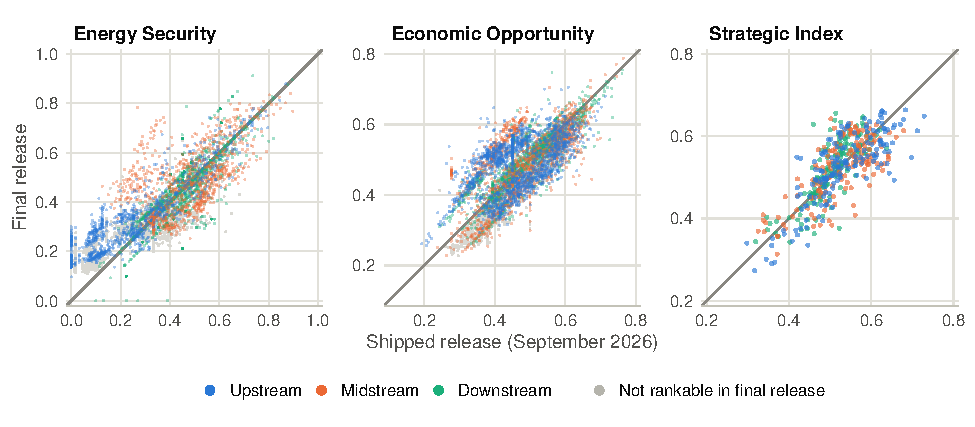
\includegraphics[width=\textwidth]{reconcile_scatter}
  \caption{Shipped against final release, cell by cell. Each point is a country--technology--stage
  cell (Energy Security, Economic Opportunity) or a country--sector cell (Strategic Index) present in
  both releases, with the shipped value (3~September 2026) on the horizontal axis and the final value
  (12~October 2026) on the vertical axis. Colour marks the stage of cells rankable in the final release
  (sovereign economy, at most half of the index weight imputed); grey points are matched cells that
  are not rankable. Energy Security: 5{,}305 matched cells, 3{,}537 rankable; Economic Opportunity:
  6{,}598 and 4{,}290; Strategic Index: the 477 cells of the 18 economies of the shipped hand-picked
  list scored in both releases. Technology--stage pairs in which a pillar is constant in either
  release are excluded. Spearman correlations over rankable cells: 0.81, 0.67 and 0.74. Shipped
  names are mapped to canonical names before matching (item C1). Sources: \texttt{index\_outputs.rds}
  of the two releases; \texttt{scripts/paper/fig\_reconcile.R}.}
  \label{fig:reconcile_scatter}
\end{figure}

A pooled correlation mixes level shifts of whole cells with reorderings within them.
Figure~\ref{fig:reconcile_cells} separates the two. The median within-cell correlation is 0.83 for
$\ES$ and 0.77 for $\EO$; 45 percent of $\ES$ values and 56 percent of $\EO$ values move by more than
ten places in their cell (median moves of 9 and 13 places). A two-factor Shapley decomposition of
each cell's change, with an unobserved shipped category counted as zero at full weight, splits it
into score effects of categories present in both releases and a composition effect from categories
that enter or leave. Composition accounts for 25 percent of the summed absolute change in $\ES$ and
40 percent in $\EO$. When the entering or leaving category is constant within a cell (the zero
Investment cells, Energy Prices, readiness) it moves the cell's level and leaves the ordering
unchanged; the reorderings come from rebuilt inputs, chiefly Foreign Dependency in the $\ES$
Upstream, Trade in the $\ES$ Midstream and Consumption or Investment in the $\ES$ Downstream. The
extreme case is $\EO$ Green Hydrogen Midstream, with a within-cell correlation of $-0.55$: both
releases rank its economies mostly on imputed values, and neither ranking should be read as a
measurement. $\ES$ Nuclear Midstream combines the largest level shift (a mean gain of 0.24, from the
removal of the zero Investment category) with a within-cell correlation of 0.59 (from the rebuilt
Trade category).

\begin{figure}[htbp]
  \centering
  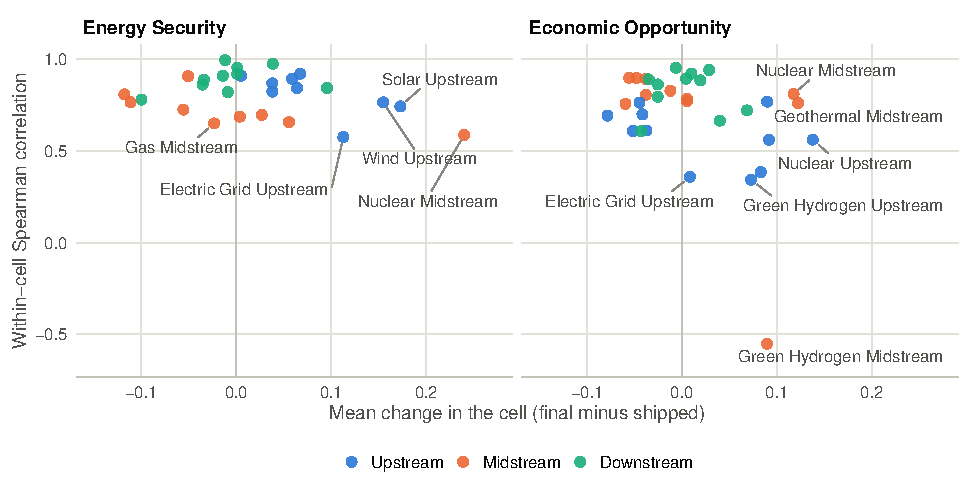
\includegraphics[width=\textwidth]{reconcile_cells}
  \caption{Level shift and rank agreement by technology--stage cell. Each point is one cell.
  Horizontal axis: mean change of the pillar (final minus shipped) across the economies scored in the
  cell in both releases and rankable in the final release. Vertical axis: Spearman correlation of the
  shipped and final values across the same economies. Colour marks the stage; labels name the three
  cells with the lowest correlation and the three with the largest absolute mean change in each panel.
  Energy Security: 28 cells (Nuclear Upstream, constant in the shipped release, is excluded;
  Geothermal Upstream and Midstream and Electric Grid Downstream have no final score; Green Hydrogen
  Midstream had no shipped one); Economic Opportunity: all 33 cells. A point far from zero
  horizontally but high vertically is a level shift that left the ordering largely intact. Sources: as
  in Figure~\ref{fig:reconcile_scatter}.}
  \label{fig:reconcile_cells}
\end{figure}

\paragraph{Coalition members.} Among the 57 members the rankable matched cells number 1{,}468
($\ES$) and 1{,}716 ($\EO$), with correlations of 0.82 and 0.68, close to the full sample.
Figure~\ref{fig:reconcile_movers} and Table~\ref{tab:reconcile_movers} show the twelve largest
changes in each pillar, at most two per cell. The largest are Canada and Namibia in Nuclear Upstream,
from zero to 0.74 and 0.72 in $\ES$: the shipped cell held only the zero Investment category, and the
Red Book places both among the leading holders and producers of uranium. The others trace the
rebuilt themes: consumption (E5), the zero-filled Investment cells (E7), the new Upstream trade
baskets, mirror trade for Gabon, which did not report imports in 2024, and the reviewed copper and
aluminium basket for the United States in Electric Grid Upstream. Eight of the twelve $\ES$ changes
and seven of the twelve $\EO$ changes are mainly composition effects, so they matter most for
comparisons across one country's cells, which is what the Strategic Index makes.

\begin{figure}[htbp]
  \centering
  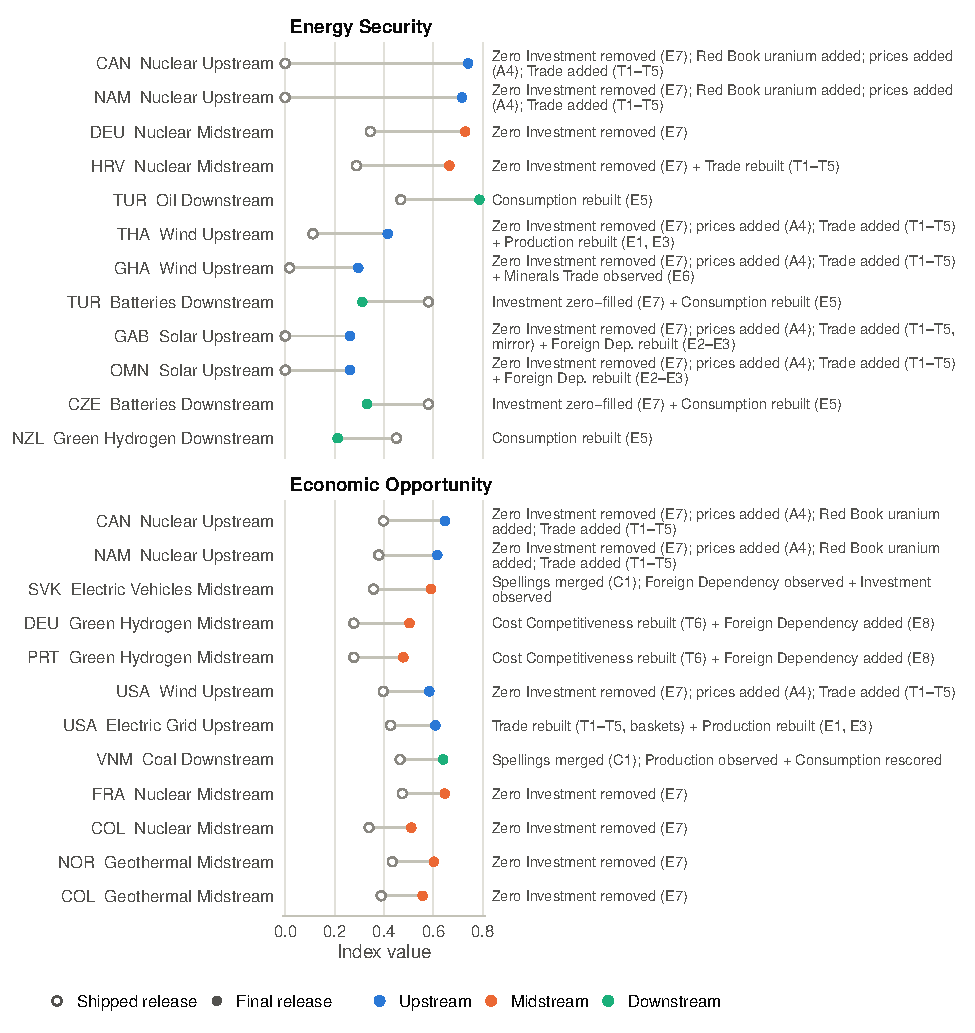
\includegraphics[width=\textwidth]{reconcile_movers}
  \caption{The twelve largest changes among coalition members, by pillar, at most two per
  technology--stage cell. Each row is one member's cell (ISO3 code). Hollow circles mark the shipped
  value and filled circles the final value, coloured by stage. The text at the right names the cause:
  the largest effect in a two-factor Shapley decomposition of the change into category score effects
  and a composition effect (categories entering or leaving and the renormalisation of weights), and
  the second when it is at least half as large, with the data change behind it (``Red Book uranium'':
  OECD-NEA/IAEA resources and production; ``mirror'': trade measured from partners' declarations).
  Item codes refer to Table~\ref{tab:corrections_index}; the full decomposition is in
  Table~\ref{tab:reconcile_movers}. Sample: the 57 members of the final coalition, cells present in
  both releases and rankable in the final release (Energy Security in Nuclear Upstream, constant in the
  shipped release, is included as a mover). Sources: \texttt{category\_contributions} of the two
  \texttt{index\_outputs.rds}.}
  \label{fig:reconcile_movers}
\end{figure}

\begingroup
  \singlespacing\scriptsize
  \setlength{\tabcolsep}{3pt}
  \setlength{\LTcapwidth}{\textwidth}
  \begin{longtable}{@{}>{\raggedright\arraybackslash}p{0.75in} >{\raggedright\arraybackslash}p{0.95in} c c c >{\raggedright\arraybackslash}p{1.05in} >{\raggedright\arraybackslash}p{1.9in}@{}}
  \caption{Largest pillar changes among coalition members and their attribution}
  \label{tab:reconcile_movers}\\
    \toprule
    Member & Cell & Shipped & Final & \makecell{Composition\\effect} & Largest score effect & Attributed cause \\
    \midrule
  \endfirsthead
    \multicolumn{7}{@{}l}{\small\textbf{Table \thetable:} continued}\\
    \toprule
    Member & Cell & Shipped & Final & \makecell{Composition\\effect} & Largest score effect & Attributed cause \\
    \midrule
  \endhead
    \bottomrule
  \endfoot
    \multicolumn{7}{@{}l}{\emph{Energy Security}} \\
    Canada & Nuclear Upstream & 0.000 & 0.741 & +0.741 & -- & Zero Investment cell removed (E7); uranium Reserves and Production added (Red Book); Energy Prices added (A4); Trade added (T1--T5; all-reporter dyads) \\
    Namibia & Nuclear Upstream & 0.000 & 0.716 & +0.716 & -- & Zero Investment cell removed (E7); uranium Reserves and Production added (Red Book); Energy Prices added (A4); Trade added (T1--T5; all-reporter dyads) \\
    Germany & Nuclear Midstream & 0.345 & 0.729 & +0.286 & Trade +0.099 & Zero Investment cell removed (E7) \\
    Croatia & Nuclear Midstream & 0.288 & 0.665 & +0.251 & Trade +0.126 & Zero Investment cell removed (E7) + Trade rebuilt (T1--T5; all-reporter dyads) \\
    Turkiye & Oil Downstream & 0.468 & 0.787 & +0.000 & Consumption +0.320 & Consumption rebuilt (E5) \\
    Thailand & Wind Upstream & 0.112 & 0.415 & +0.127 & Production +0.123 & Zero Investment cell removed (E7); Energy Prices added (A4); Trade added (T1--T5; all-reporter dyads) + Production rebuilt (E1, E3) \\
    Ghana & Wind Upstream & 0.018 & 0.296 & +0.105 & Minerals Trade +0.088 & Zero Investment cell removed (E7); Energy Prices added (A4); Trade added (T1--T5; all-reporter dyads) + Minerals Trade observed, was imputed (E6) \\
    Turkiye & Batteries Downstream & 0.580 & 0.312 & +0.000 & Investment $-$0.165 & Investment zero-filled (E7) + Consumption rebuilt (E5) \\
    Gabon & Solar Upstream & 0.000 & 0.263 & +0.105 & Foreign Dependency +0.086 & Zero Investment cell removed (E7); Energy Prices added (A4); Trade added (T1--T5; all-reporter dyads, mirror imports) + Foreign Dependency rebuilt (E2--E3) \\
    Oman & Solar Upstream & 0.000 & 0.262 & +0.090 & Foreign Dependency +0.086 & Zero Investment cell removed (E7); Energy Prices added (A4); Trade added (T1--T5; all-reporter dyads) + Foreign Dependency rebuilt (E2--E3) \\
    Czech Republic & Batteries Downstream & 0.580 & 0.331 & +0.000 & Investment $-$0.165 & Investment zero-filled (E7) + Consumption rebuilt (E5) \\
    New Zealand & Green Hydrogen Downstream & 0.451 & 0.212 & +0.000 & Consumption $-$0.238 & Consumption rebuilt (E5) \\
    \addlinespace
    \multicolumn{7}{@{}l}{\emph{Economic Opportunity}} \\
    Canada & Nuclear Upstream & 0.398 & 0.647 & +0.266 & Technology Demand $-$0.015 & Zero Investment cell removed (E7); Energy Prices added (A4); Production added (E1, E3; uranium, Red Book); Trade added (T1--T5; all-reporter dyads) \\
    Namibia & Nuclear Upstream & 0.379 & 0.616 & +0.257 & Cost Competitiveness $-$0.016 & Zero Investment cell removed (E7); Energy Prices added (A4); Production added (E1, E3; uranium, Red Book); Trade added (T1--T5; all-reporter dyads) \\
    Slovak Republic & Electric Vehicles Midstream & 0.358 & 0.591 & +0.000 & Foreign Dependency +0.148 & Spellings merged (C1); Foreign Dependency observed + Investment observed \\
    Germany & Green Hydrogen Midstream & 0.278 & 0.503 & +0.066 & Cost Competitiveness +0.098 & Cost Competitiveness rebuilt (T6) + Foreign Dependency added (E8) \\
    Portugal & Green Hydrogen Midstream & 0.278 & 0.479 & +0.070 & Cost Competitiveness +0.118 & Cost Competitiveness rebuilt (T6) + Foreign Dependency added (E8) \\
    United States & Wind Upstream & 0.397 & 0.584 & +0.164 & Production +0.064 & Zero Investment cell removed (E7); Energy Prices added (A4); Trade added (T1--T5; all-reporter dyads) \\
    United States & Electric Grid Upstream & 0.427 & 0.608 & +0.069 & Trade +0.079 & Trade rebuilt (T1--T5; all-reporter dyads, basket review) + Production rebuilt (E1, E3) \\
    Viet Nam & Coal Downstream & 0.465 & 0.640 & +0.000 & Production +0.052 & Spellings merged (C1); Production observed + Consumption rescored \\
    France & Nuclear Midstream & 0.474 & 0.647 & +0.124 & Trade +0.034 & Zero Investment cell removed (E7) \\
    Colombia & Nuclear Midstream & 0.340 & 0.511 & +0.094 & Trade +0.044 & Zero Investment cell removed (E7) \\
    Norway & Geothermal Midstream & 0.434 & 0.602 & +0.148 & Cost Competitiveness +0.038 & Zero Investment cell removed (E7) \\
    Colombia & Geothermal Midstream & 0.389 & 0.557 & +0.134 & Cost Competitiveness +0.050 & Zero Investment cell removed (E7) \\
  \end{longtable}
  \vspace{-6pt}\footnotesize\noindent
    \emph{Notes:} The 12 largest absolute changes, final minus shipped release, of $\ES_{its}$ and of $\EO_{its}$ among the 57 members of the final coalition, at most 2 per technology--stage cell, over the headline cells present in both releases that the final release ranks (sovereign economy, at most half of the index weight imputed); cells that were constant across countries in the shipped release are included. The change is split by a two-factor Shapley decomposition of the weighted category mean: the score effect of a category present in both releases is $\tfrac12(\omega^{\text{shipped}}_k+\omega^{\text{final}}_k)(c^{\text{final}}_k-c^{\text{shipped}}_k)$, with $\omega_k$ the normalised category weight and an unobserved shipped category counted as $c_k=0$ (item A1); the composition effect is the remainder, due to categories that enter or leave and to the renormalisation of the weights. The cause names the largest effect, and the second when it is at least half as large; item codes refer to Table~\ref{tab:corrections_index}. Data changes: ``uranium, Red Book'' = identified recoverable resources and mine production of the OECD-NEA/IAEA Red Book; ``USGS MCS 2026'' = critical-mineral reserves of the USGS Mineral Commodity Summaries 2026; ``all-reporter dyads'' = trade rebuilt from all-reporter Comtrade dyads (importer report first, else the exporter's declaration $\times 1.06$) and the energy-trade file rebuilt from the same pull; ``basket review'' = a stage whose HS6 basket the October 2026 review changed; ``mirror imports'' = an economy that did not report 2024 imports, whose imports come from partners' declarations; ``TRL by stage'' = technology readiness mapped by stage from the IEA Clean Technology Guide. Source: \texttt{category\_contributions} of the two \texttt{index\_outputs.rds}.\par
\endgroup
\medskip


\paragraph{Strategic Index.} The shipped index scored 571 cells of 18 economies of its hand-picked
list; the final one scores 3{,}154 cells of 174 countries in 30 sectors. On the 477 cells scored in
both the correlation is 0.74, and across sectors within a country the median is 0.74 (Argentina 0.42
to Kenya 0.92). The policy term changed most. The shipped Policy index combined IEA PAMS, CAT, the
February 2026 NIPO component and the dual-use score; the final one combines IEA PAMS and CAT, and all
18 economies have both. The within-country policy term correlates only 0.61 between releases and
accounts for 40 percent of the summed absolute change, against 35 percent for security need, 22
percent for $\EO$ and 3 percent for the fixed weights, which differ only through the technology
weights of oil (0.12 shipped, 0 final) and coal (0 and 0.02; item P9). In the final run 215
countries are policy-eligible (65 on IEA PAMS and CAT, 150 on IEA PAMS alone); all 23 economies of
the shipped hand-picked list are among them, as are all 57 members of the derived coalition.
Figure~\ref{fig:reconcile_si_terms} splits the twelve largest changes into their terms. For the final
release Geothermal Midstream is excluded by rule, as before; no sector is constant in either pillar,
because Nuclear Upstream now varies with the Red Book data; and Electric Grid Downstream and
Geothermal Upstream have no $\ES$ value, so the index covers 30 sectors.

\begin{figure}[htbp]
  \centering
  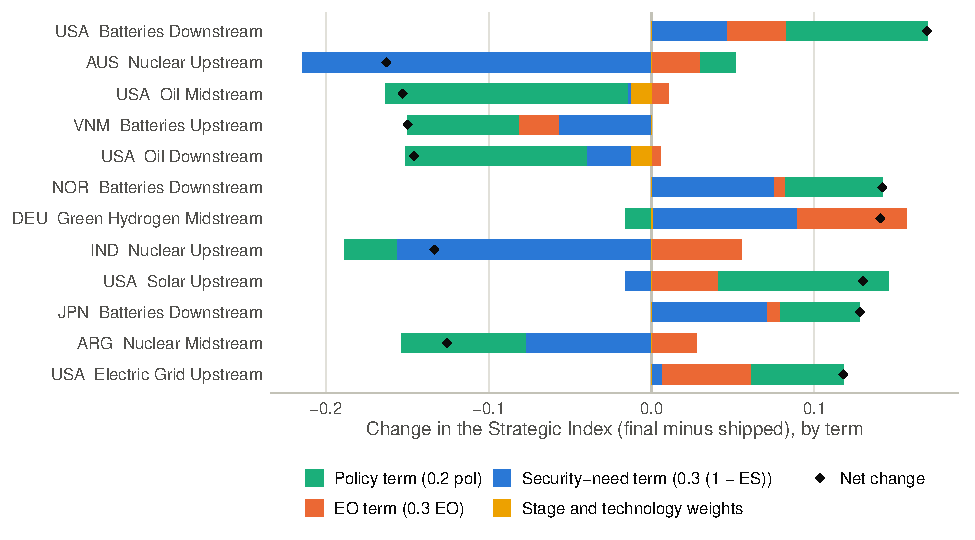
\includegraphics[width=\textwidth]{reconcile_si_terms}
  \caption{The twelve largest changes in the Strategic Index among the economies scored in both
  releases, split into the weighted terms of $\SI=0.2\,\POL+0.3\,\EO+0.3\,(1-\ES)+0.1\,\lambda_s+0.1\,g_t$.
  Each bar is one country--sector cell; the segments are the changes of the policy term, the $\EO$
  term, the security-need term and the two fixed weights combined, and the diamond is the net change,
  which the segments sum to exactly. The shipped policy term is the within-country S-curve of the
  four-component Policy index of February 2026 (IEA PAMS, CAT, NIPO, dual use); the final one is that
  of IEA PAMS and CAT. The policy term is the largest contributor in seven of the twelve, security need
  in five. Sample: the 477 cells of the 18 economies of the shipped hand-picked list scored in both
  releases. Sources: \texttt{strategic\_index} of the two \texttt{index\_outputs.rds};
  \texttt{scripts/paper/fig\_reconcile.R}.}
  \label{fig:reconcile_si_terms}
\end{figure}

\paragraph{The allied picks.} The shipped picks were made over a hand-picked list of 23 economies,
the final ones over the 57 members of the derived coalition, so the comparison covers the 21 they
share (Table~\ref{tab:reconcile_allied}). Kenya and the United Arab Emirates are not members of the
final coalition, and Denmark, France, Italy and South Korea had no shipped pick because they lacked
a Policy index (P3). Of the 17 members with a pick in both releases, 16 change it; only Chile keeps
Nuclear Upstream. Six changes (Australia, Brazil, Canada, India, Mexico and the United States) are
reorderings by the security-need term: all six picked Nuclear Upstream where the shipped $\ES$ was
zero for everyone, and the Red Book now records uranium for all six. Four (Argentina, Indonesia,
South Africa, Viet Nam) are reorderings by the policy term, four (Germany, Japan, Morocco, Norway)
are barred by the endowment screen, and two (Saudi Arabia, the United Kingdom) are no longer scored
because the $\EO$ cell of the shipped pick is not rankable. On these members the picks move from
Nuclear Upstream (8) and Batteries Upstream (5) to Batteries Midstream (13).

\begin{table}[htbp]
  \centering
  \begin{threeparttable}
  \caption{Allied pick per member of the shipped list: shipped and final release}
  \label{tab:reconcile_allied}
  \footnotesize
  \begin{tabularx}{\textwidth}{@{}l >{\raggedright\arraybackslash}p{1.15in} c >{\raggedright\arraybackslash}p{1.15in} c >{\raggedright\arraybackslash}X@{}}
    \toprule
    & \multicolumn{2}{c}{Shipped release} & \multicolumn{2}{c}{Final release} & \\
    \cmidrule(lr){2-3}\cmidrule(lr){4-5}
    Member & Pick & $\SI$ & Pick & $\SI$ & Status or cause of change \\
    \midrule
    Argentina & Electric Vehicles, Midstream & 0.624 & Batteries, Upstream & 0.551 & reordered by the policy term \\
    Australia & Nuclear, Upstream & 0.656 & Batteries, Midstream & 0.610 & reordered by the security-need term \\
    Brazil & Nuclear, Upstream & 0.613 & Batteries, Midstream & 0.606 & reordered by the security-need term \\
    Canada & Nuclear, Upstream & 0.638 & Electric Grid, Midstream & 0.615 & reordered by the security-need term \\
    Chile & Nuclear, Upstream & 0.626 & Nuclear, Upstream & 0.645 & unchanged \\
    Denmark & -- & -- & Batteries, Midstream & 0.636 & new \\
    France & -- & -- & Batteries, Midstream & 0.642 & new \\
    Germany & Batteries, Upstream & 0.712 & Batteries, Midstream & 0.623 & shipped pick screened: no resource base \\
    India & Nuclear, Upstream & 0.643 & Batteries, Midstream & 0.628 & reordered by the security-need term \\
    Indonesia & Electric Vehicles, Midstream & 0.642 & Nuclear, Midstream & 0.568 & reordered by the policy term \\
    Italy & -- & -- & Batteries, Midstream & 0.639 & new \\
    Japan & Batteries, Upstream & 0.657 & Nuclear, Upstream & 0.620 & shipped pick screened: no resource base \\
    Kenya & Batteries, Upstream & 0.701 & \emph{not a member} & -- & not in final coalition \\
    Mexico & Nuclear, Upstream & 0.624 & Batteries, Midstream & 0.564 & reordered by the security-need term \\
    Morocco & Solar, Upstream & 0.683 & Electric Grid, Midstream & 0.609 & shipped pick screened: no resource base \\
    Norway & Nuclear, Upstream & 0.729 & Batteries, Upstream & 0.618 & shipped pick screened: no resource base \\
    Saudi Arabia & Batteries, Upstream & 0.688 & Nuclear, Upstream & 0.567 & shipped pick not scored: EO not rankable \\
    South Africa & Electric Grid, Midstream & 0.679 & Batteries, Midstream & 0.620 & reordered by the policy term \\
    South Korea & -- & -- & Batteries, Midstream & 0.635 & new \\
    United Arab Emirates & -- & -- & \emph{not a member} & -- & not in final coalition \\
    United Kingdom & Batteries, Upstream & 0.690 & Batteries, Midstream & 0.617 & shipped pick not scored: EO not rankable \\
    United States & Nuclear, Upstream & 0.613 & Batteries, Midstream & 0.632 & reordered by the security-need term \\
    Viet Nam & Batteries, Upstream & 0.698 & Batteries, Midstream & 0.606 & reordered by the policy term \\
    \bottomrule
  \end{tabularx}
  \begin{tablenotes}[flushleft]\footnotesize
    \item \emph{Notes:} The pick is the member's Upstream or Midstream sector with the highest Strategic Index; Geothermal and Green Hydrogen are excluded by rule of the selection. Shipped release: the Strategic Index of 3~September 2026 over its hand-picked list of 23 economies, of which 18 had a pick. Final release: \texttt{data/processed/charts/allied\_strategic.csv}, over the derived coalition of 57 members, with the endowment screen (an Upstream extraction stage is eligible only where the member has recorded reserves or production of its resources). The comparison is on the 21 members the two lists share; 2 economies of the shipped list are not in the final coalition. ``new'': a pick only in the final release. Cause of a change: the shipped pick is no longer scored (its exclusion), is barred by the endowment screen, or is outscored, in which case the term of the index that contributes most to the reversal of the two sectors' order is named (an exact split of the reversal into the five weighted terms). The picks of the other 36 final members are reported in Section~\ref{sec:strategic}.
  \end{tablenotes}
  \end{threeparttable}
\end{table}


\paragraph{Network and partnership strength.} The shipped network outputs are not comparable with
the final ones (Table~\ref{tab:reconcile_network}). The shipped diagnostics record a greedy solution
in all 33 stages over 22 effective members, and in 14 stages a producer count of $k^2$ with a
Herfindahl index of one, the signature of \eqref{eq:corr_fanout}; the portfolio loop stopped at its
limit with 12 members above their caps. The final design solves 22 stages over 37 nodes by MILP, with
7 to 10 producers per stage and a median designed Herfindahl index of 0.152, and the loop converges
in seven passes. The shipped release did not write the PSI to disk; reconstructed from the March 2026
partner tables with the shipped logic, it correlates $-0.09$ with the final world view over 187
partners and $-0.33$ with the core view over 191. The denominator defect (B4) placed high-income
partners below the others, so correcting it moves that group up as a block: the United States moves
from 168th to 4th of the 187 in the world view and to 1st in the core view, and Germany from 135th to
5th. China moves from 22nd to 1st in the world view but to 44th in the core view, whose Friendshore
scores rate China from the core members' viewpoints, alignment included.

\begin{table}[htbp]
  \centering
  \begin{threeparttable}
  \caption{Allied network diagnostics: shipped and final release}
  \label{tab:reconcile_network}
  \small
  \begin{tabular}{@{}l c c@{}}
    \toprule
    & Shipped release & Final release \\
    \midrule
    Network nodes & 22 & 37 \\
    Stages designed & 33 (all three stages) & 22 (Upstream, Midstream) \\
    Solver used (stages) & greedy (33) & MILP (22) \\
    Stages with $n_{\text{producers}}=k^2$ and $\HHI=1$ & 14 & 0 \\
    Reported producers per stage & 3--193{,}600 & 7--10 (median 9) \\
    $\HHI$ of designed shares & 0.333--1.000 & 0.126--0.209 (median 0.1520) \\
    Diversification weight $\lambda$ & -- & 0.78 \\
    Policy term in node scores & yes & no \\
    Portfolio loop converged & no & yes \\
    Portfolio passes & 10 (limit) & 7 \\
    Members above their portfolio cap at exit & 12 & 0 \\
    \bottomrule
  \end{tabular}
  \begin{tablenotes}[flushleft]\footnotesize
    \item \emph{Notes:} Shipped release: \texttt{allied\_network\_diagnostics.csv} written on 23~February 2026, the only shipped network artefact read here; it designed every stage of the hand-picked list's 22 effective members (the United Arab Emirates was coded ``UAE'', item N5). In 14 shipped stages a single country was selected with $k^2$ rows of share $1/k$, so the producer count was $k^2$ (with $k$ from 16 to 440) and the Herfindahl index summed over the rows was exactly one (item N1, equation~\eqref{eq:corr_fanout}). Final release: the same file of the final run of 12~October 2026, 37 nodes (the EU-27 as one node), Upstream and Midstream stages only, MILP with the concave diversification term ($\lambda=0.78$, the smallest value on the calibration grid whose median designed $\HHI$ does not exceed the observed one) and portfolio caps, and no policy term in the node scores; the median designed $\HHI$ compares with a median observed export $\HHI$ of the nodes of 0.1556 over the 18 stages with an HS6 basket. The portfolio loop runs over all stages jointly, so it has one outcome per release; the last row counts the members that, when the loop stops, are a top producer in more stages than their cap allows.
  \end{tablenotes}
  \end{threeparttable}
\end{table}


\paragraph{Using numbers from the shipped release.} Within a technology--stage cell, shipped pillar
rankings are a rough guide in the Downstream (median within-cell correlations 0.90 for $\ES$ and 0.88
for $\EO$) and in the $\EO$ Midstream (0.80), a poor guide in the $\ES$ Midstream (0.70) and the $\EO$
Upstream (0.61), and no guide for $\EO$ Green Hydrogen Midstream. Comparisons across cells, and with
them the shipped Strategic Index and its picks, inherit the level shifts and a different Policy index;
the shipped picks should be replaced by those of Section~\ref{sec:strategic}. The shipped network
outputs and any PSI computed from the shipped partner tables should not be used. As the
composite-indicator literature warns, the ordering a composite produces can depend on its
construction as much as on its data \citep{saisana2005uncertainty,saltelli2007composite}; here,
however, the large changes come from defects and new data rather than from defensible alternative
choices, so they are corrections, not a measure of uncertainty.

\end{appendices}

% ---------------------------------------------------------------------------
% Online Appendix (sections in the order of the main text)
% ---------------------------------------------------------------------------
\startonlineappendix
% Online Appendix to Section 3 (sec:data). Specification: scripts/utils/raw_inputs.R
% (resolve_versioned_raw_input), config/raw_inputs_manifest.yml, data/raw/raw_inputs_resolved.yml,
% R/utils/country.R, R/utils/eia_intl.R, scripts/98_pull_comtrade_energy_dyads.R,
% scripts/40_build_index_vintages.R, docs/methodology.md. Final rerun of 12 October 2026.
\section{Data: releases, harmonisation and years}\label{oa:data}

\paragraph{The release rule.} Inputs that are published in successive releases are staged under
a file-name pattern, and the run selects one release by rule rather than by hand. Let $F_P$ be the
staged files matching the pattern of input $P$, $k(f)$ the vintage key parsed from a file's name
(a date or a year), $m(f)$ its modification time and $R(f)$ the number of distinct reporters in a
tabular extract. The release used is
\begin{equation}\label{eq:data_resolve}
  f^{*}_{P}=\operatorname*{lex\,max}_{f\in F_P:\ R(f)\ge\underline R_P}\ \bigl(k(f),\,m(f)\bigr),
\end{equation}
the newest declared vintage, with the modification time breaking ties and ordering unversioned
names, among the files that meet the coverage floor $\underline R_P$. The floor is 50 reporters for
the Comtrade critical-minerals extracts and absent elsewhere. Comtrade publishes a year's data as
reporters file, so the newest file can be a stub: the 2025 critical-minerals extracts have three
reporters each and are skipped in favour of the 2024 extracts (130 import, 128 export and 130
total-export reporters). Every run writes the releases it resolved, with their reporter counts, to
a vintage stamp (\texttt{data/raw/raw\_inputs\_resolved.yml}); Appendix~\ref{app:sources} reports
them. Inputs that are not pattern-resolved (the Comtrade dyads, the Red Book and USGS tables, the
EIA bulk file, CM-FDI, the ideal points and the project-authored lists) are single staged files
whose access dates are recorded in the input manifest.

\paragraph{Harmonisation of economies.} Every source is put on one canonical name per economy
before anything is ranked: the World Development Indicators name of the economy's ISO3 code,
matched through the \texttt{countrycode} package and a curated table of spellings. Taiwan, which the
World Bank's country table does not list, is added under its own code, including to the rosters of
the trade themes; Kosovo is carried as XKX. World, regional, income-group and residual rows
(``Other Asia Pacific'', ``Rest of world'') and historical entities are dropped from every theme
table, so that no aggregate is imputed or averaged as if it were an economy; theme builders also
remove aggregates from their comparison sets before ranking, while keeping them in world
denominators where the source defines the world total. Keys that two spellings of one economy
share are collapsed, with a warning if both carry different non-missing values. Sovereignty, which
the rankability rule uses, follows the Correlates of War state-system list \citep{cow2024state}:
195 states in 2024, the 193 UN members plus Kosovo and Taiwan.

\paragraph{Fossil production from EIA.} The Statistical Review lists fewer producers than consumers
and counts the rest in regional ``Other'' residuals. Where it has no production row for an economy
and fuel, the value is taken from the EIA International Energy Statistics \citep{eia2026international}
(bulk file of 3 October 2026) in the Review's units: oil as crude oil including lease condensate
plus natural-gas plant liquids, in thousand barrels a day; gas as dry gas in billion cubic metres
times 0.036 EJ; coal as terajoules (gross calorific value) times $0.95\times10^{-6}$ EJ. On economies
both sources report, the median ratio of the Review's value to the converted EIA value is 1.006 to
1.011 for oil, 0.97 to 0.99 for gas and 0.99 to 1.05 for coal. An EIA value is not used when EIA's
consumption of the fuel covers less than a tenth of the Review's, since the Review then counts under
the fuel something EIA excludes; in 2015--2025 this affects only Estonian coal (oil shale), which
stays missing. Where EIA's latest production year precedes the Review's consumption year (2025 gas
and coal from EIA 2024), self-sufficiency is computed with consumption of the same year and carried
forward. EIA values are observations, not imputations.

\paragraph{Reserves and uranium.} The USGS Mineral Commodity Summaries 2026 data release
\citep{usgs2026mcs} gives country reserves at end-2025; the report's version 1.3 erratum puts
Brazil's rare-earth reserves at 11~Mt (the Statistical Review's mineral sheet, an older USGS copy,
gives 21~Mt). A reported zero scores 0; a holder listed without a figure (NA, W or s) is missing in
its mineral variable, scored 0 and counted as imputed, and counts as zero in the technology
roll-ups, so world shares are measured on quantified holdings. ``Other countries'' and world-total
rows are never holders. The Red Book \citep{oecdnea2026uranium} supplies identified recoverable
resources (reasonably assured plus inferred) below USD 260/kgU at 1 January 2025 (Table 1.2a of
\emph{Uranium 2026}) and mine production (Table 1.18; \emph{Uranium 2026} for 2022--2024, earlier
editions for 2019--2021), completed with observed zeros over the economies of the Statistical
Review and the World Development Indicators.

\paragraph{Bilateral trade.} The all-reporter dyad file was pulled on 7--8 October 2026 for the
pre-review product list, with supplements on 9 October (the copper and aluminium inputs of the grid)
and 12 October (the new upstream codes). Comtrade's partner S19 (``Other Asia, n.e.s.'') is mapped
to Taiwan. Liberia, Mali and S\~ao Tom\'e and Pr\'incipe filed 2024 data after the pull and enter
through their partners' declarations. The country-level energy-trade file is derived from the
pull's World rows; an earlier direct extract, with 129--130 reporters, lacked 60 basket codes and
Qatar's exports of liquefied natural gas. Critical-minerals exports of non-reporting economies are
measured from partners' imports, moved from CIF to FOB with an HS-chapter ratio estimated on
importers that file both values.

\paragraph{Regional and staged inputs.} The IEA's 2035 announced manufacturing-capacity shares and
its electric-vehicle production and sales are regional for Europe, so EU members carry the EU's
value; economies outside the IEA's named regions take its ``Rest of world'' values. ILOSTAT
earnings are read from a copy staged on 30 September 2026, since the ILO's interface returns empty
responses to scripted requests. In the IMF lending-rate series a zero reading in a lending-type
rate is a placeholder and is dropped with the averages that include it: New Zealand's lending series
carries only zeros after January 2017, so its last genuine reading (4.76 percent) is used. Commodity
prices are in the units of the IMF series metadata.

\begin{table}[tbp]
\centering
\begin{threeparttable}
\caption{Years of the inputs in the final run}\label{tab:oa_data_years}
\footnotesize
\begin{tabularx}{\textwidth}{@{}>{\raggedright\arraybackslash}p{5.2cm} >{\raggedright\arraybackslash}X@{}}
\toprule
Source & Years used\\
\midrule
EI Statistical Review 2026 & Consumption and production to 2025 (growth 2020--2025); fossil
  reserves end-2020\\
EIA International Energy Statistics & Oil production to 2025; gas and coal to 2024\\
USGS Mineral Commodity Summaries 2026 & Reserves end-2025\\
Red Book (Uranium 2026) & Resources at 1 January 2025; production 2019--2024\\
IEA Critical Minerals Dataset 2026 & Base year and 2035 (Stated Policies)\\
IEA ETP 2024 capacity; IEA EV regional data & Announced capacity to 2035; EV production and sales
  2024\\
UN Comtrade dyads; energy-trade file & 2020 and 2024; 2024\\
Comtrade critical-minerals extracts & 2024 (2025 below the floor)\\
Atlas of Economic Complexity (HS92) & 2023\\
IEA WEO 2025; Global EV Outlook 2026 & 2024 and 2035; 2022, 2025 and 2035\\
BNEF New Energy Outlook 2024; Supply Chains 2025 & 2024 and 2035; 2025\\
IEA Clean Energy Technology Guide 2026 & Readiness 2020--2025\\
BNEF LCOE; IEA relative costs & 2025 and 2050; 2023\\
ILOSTAT; IMF lending rates, PPI, PCPS & Latest within ten years; to October, September and
  December 2025\\
Clean Investment Monitor & Investment 2018--2025; capacity 2025\\
IEA PAMS; Climate Action Tracker & Export of 22 January 2026; ratings of May 2022--June 2025\\
IMF Direct Investment Positions; CM-FDI & Mean of 2020--2024; edition of 5 October 2026\\
WDI; Doing Business; OECD CRS & 2022--2024 (GDP to 2025); 2019; 2013--2024\\
UNGA ideal points (Dataverse V39) & Sessions 74--78 (2019--2023)\\
\bottomrule
\end{tabularx}
\begin{tablenotes}[flushleft]\footnotesize
\item \textit{Notes:} Each component enters at the latest year its source reports
(equation~\eqref{eq:latest_year}). Appendix~\ref{app:sources} gives the releases.
\end{tablenotes}
\end{threeparttable}
\end{table}

\paragraph{Index vintages.} The headline indices are a single snapshot. A separate build re-cuts
each raw input to a requested year and reruns the same theme and pillar builders, so that the
pillars can be compared across years (Section~\ref{sec:robustness}). Only sources with a genuine
time dimension move: the Statistical Review, the Atlas trade data, IMF prices and rates, ILOSTAT
earnings and Clean Investment Monitor investment. Resource potential, reserves, the IEA critical
minerals release, BloombergNEF demand and costs, overcapacity and technology readiness are
snapshots or projections and are held fixed; a 2025 vintage uses Atlas 2023. The build records,
for each vintage, the share of each pillar's scored weight that re-derives and the year to which
each source resolved.

% Online Appendix to Section 4 (sec:normalization). Specification: R/utils/scurve.R,
% R/indices/index_builder_core.R, config/index_definition.yml, config/missing_data.yml,
% config/weights.yml, config/rankability.yml. Numbers: paper/results/method.json and scurve.json
% (final rerun of 12 October 2026).
\section{Index construction: derivations and further diagnostics}\label{oa:normalization}

This appendix collects the construction algorithm, the properties of the S-curve that Section~\ref{sec:normalization}
uses without proof, the conventions of the theme and aggregation layers, and the diagnostics of
the final build that the main text summarises.

\begin{algorithm}[t]
  \caption{Construction of a pillar index $P\in\{\ES,\EO\}$ from its theme tables}
  \label{alg:pillar}
  \begin{algorithmic}[1]
    \Require theme tables $h\in\mathcal H_P$; category weights $w_k$
      (\texttt{config/weights.yml}); missing-data rules $m_h\in\{\text{zero},
      \text{global average}\}$ (\texttt{config/missing\_data.yml}); for each category its
      score variable and components $\mathcal V_{k}$ (\texttt{config/index\_definition.yml})
    \State Bind the theme tables; average rows that differ only by sub-sector; keep rows whose
      data type is \emph{index}
    \State For each $(i,t,s,k,v,h)$ keep the observation with the latest year
      \Comment{eq.~\eqref{eq:latest_year}}
    \For{each technology--stage pair $(t,s)$}
      \State Complete the grid of economies $\times$ component groups
      \For{each group $g=(t,s,k,v,h)$}
        \If{at least one economy is observed in $g$ and theme $h$ has a rule}
          \State Fill the missing economies of $g$ by rule $m_h$ from the observed values
          \Comment{eq.~\eqref{eq:impute}}
        \EndIf
      \EndFor
    \EndFor
    \State Average each component over themes; score each category by the mean of its present
      components \Comment{eq.~\eqref{eq:overall}}
    \State Aggregate the observed categories of each cell with renormalised weights
      \Comment{eq.~\eqref{eq:pillar}}
    \State Record category and variable contributions, $\iota_{its}$ and the pair status; flag
      rankable cells \Comment{eqs.~\eqref{eq:cat_decomp}--\eqref{eq:rankable}}
    \Ensure $P_{its}\in[0,1]$, or missing when no category of the cell is observed
  \end{algorithmic}
\end{algorithm}

\paragraph{Theme tables and orientation.} Every theme table has one row per economy, technology,
stage, sub-sector, category, variable, data type and year, with its value, source and a short
explanation. Rows of type \emph{raw} keep a metric in natural units for tracing; only rows of type
\emph{index}, on $[0,1]$, enter the pillars. Rows that differ only by sub-sector are averaged with
equal weights before any other step. Each variable is oriented in its theme: concentration enters
through $-\HHI$, a trade deficit relative to GDP, a levelised cost and price volatility through
their negatives. By the symmetry of $\Scurve$, the S-curve of $-x$ is one minus the S-curve of $x$
for any comparison set with at least two observations, so orientation and transformation commute.
The opportunity builder verifies that every category score lies in $[0,1]$.

\paragraph{The S-curve.} Differentiating equation~\eqref{eq:scurve},
\begin{equation}\label{eq:scurve_slope}
  \Scurve'(r)=\frac{\gamma\,[r(1-r)]^{\gamma-1}}{\bigl[r^{\gamma}+(1-r)^{\gamma}\bigr]^{2}},
  \qquad \Scurve'(1/2)=\gamma ,
\end{equation}
which for $\gamma<1$ diverges as $r\to0$ or $r\to1$. With $\gamma=0.5$ the quartiles map to
0.366 and 0.634, so near the median a step in rank moves the index by half as much as it moves the
percent rank, while gaps between adjacent units are widened in the tails. In levels, $\Scurve(r)>r$
below the median and $\Scurve(r)<r$ above it. With $n$ untied observations the index takes exactly
the values $\Scurve(k/(n-1))$, $k=0,\dots,n-1$, whatever the raw distribution, so every untied
S-curved variable has mean $1/2$ and a dispersion that depends only on $n$ and $\gamma$: the
population standard deviation is 0.260 for $n=10$, 0.224 for $n=20$ and 0.206 for $n=40$, and
tends to 0.19, against 0.29 for the percent rank and 0.38 for $\gamma=2$. Components ranked over
comparison sets of a given size therefore enter a category on a common scale; smaller sets have
larger spreads, and ties, the zero anchor and imputed values move a component away from the grid.
The smallest step above zero, $\Scurve(1/(n-1))$, is coarse in small sets (0.261 for $n=10$,
0.140 for $n=40$). A single observation scores 0, two score 0 and 1, and a fully tied set scores
$1/2$. In the simulated lognormal sample of Figure~\ref{fig:scurve}, min-max rescaling puts 29 of
40 observations below 0.1 and spreads the top four over 0.79 of the scale; the percent rank gives
each group of four a spread of 0.077; the S-curve gives the bottom and top four 0.22 each and the
middle four 0.04. Rank-based normalisation is a standard option for composite indicators
\citep{oecd2008handbook}; it is adopted because the inputs differ in units and skewness by orders
of magnitude and the questions the indices answer are comparative. Min-max or $z$-score
normalisation would let a few very large values compress the rest of the distribution.

\paragraph{The zero anchor.} Equation~\eqref{eq:scurve_zero} is equation~\eqref{eq:scurve}
applied to the positive values with a single zero prepended to the comparison set and then
removed. An observed zero and an unrecorded economy both score 0, and the smallest positive value
scores $\Scurve(1/m)>0$: for $(0,2,5,9)$ the positive entries score 0.414, 0.586 and 1. A set in
which every value is zero scores 0 throughout.

\paragraph{Comparison sets and cardinal exceptions.} Most themes rank the economies observed in a
pair, sometimes split by sub-sector, year or mineral before averaging to the pair. World-level
series are ranked across the units over which they vary: commodity-price volatility across
technologies, world export concentration across the cells of the eleven headline technologies, and
global demand across fuels. A theme that builds a composite of several S-curved terms averages
them and may pass the average through the S-curve again. Index values are positions in a
cross-section: adding or removing economies changes the scores of the others, and a change over
time records a change in standing against the field. The three cardinal $\EO$ inputs are the
readiness score (a raised-cosine bell in the readiness level, zero at levels 2 and 11 and peaking
at 6, blended 0.7:0.3 with a capped concave score of its recent increase), the overcapacity term
$2^{-\rho}$ in BloombergNEF's ratio $\rho$ of capacity to forecast demand, and the capital-cost
term of the input-cost index, a lending rate winsorised at its 5th and 95th cross-country
percentiles and rescaled by min-max. They keep interval information and do not share the fixed
distribution of an S-curved variable; the first two are technology-level values.

\paragraph{Latest year.} The selection of equation~\eqref{eq:latest_year} is made on the year
field, with undated rows at year 0, separately for each economy and variable. A row recorded for a
later year with a missing value therefore supersedes an earlier observed value. In $\ES$ the mixed
years lie between 2023 and 2025, apart from the 2035 horizon of the announced manufacturing-capacity
shares. In $\EO$ part of the mixing reflects the projection horizons of the outlook series;
counting only years up to 2026, 91 percent of $\EO$ cells still combine more than one vintage, with
at most four years and a median spread of three among the cells that mix. The extreme case is the
input-cost index of Papua New Guinea, whose latest observation is for 1980 and which enters all 33
of its $\EO$ cells through Cost Competitiveness.

\paragraph{The grid and the rules.} Because a pair's grid is the union of the economies of all the
pillar's themes for the pair, one broadly distributed theme sets its extent: the commodity-price
series is copied to every economy of the World Bank list at the upstream stage, so every such
economy enters the upstream grid of each technology with a price series and is scored there on its
other components, observed or filled. Rows of categories a pillar does not score cannot add
economies to its grid. Every one of the 219 economies in the upstream grids has a country-specific
upstream component in at least one upstream pair of each pillar. When a single economy is observed
in a group, the global-average rule copies its value to every other economy: this is how the Boston
Consulting Group estimate of the U.S. serviceable addressable market, one value per pair, enters
$\EO$ Technology Demand, flagged as imputed for every economy but the United States. Because the
average is taken after the latest-year selection, it can combine observations of different years.
The zero rule equates ``not recorded'' with ``none'' and so understates the position of an economy
an incomplete register omits.

\paragraph{Overall variables.} A component reported by several themes (energy consumption per
capita, for example) is averaged across them with equal weights before the category mean. Some
component lists follow a one-vote-per-source principle: where a source enters through a composite
of its own terms, the composite is one component. Two checks guard the mapping from configuration
to data: the builder warns when none of a category's listed components occurs in the inputs, and
it discards any theme row that carries the name of a configured overall variable, so the
configured definition always governs. A configuration test requires the weighted categories of each
pillar to coincide with its configured categories.

\paragraph{Why not zero-fill.} Replacing each unobserved category by the cell's available-case
mean and averaging over all categories with the nominal weights returns $\ES_{its}$ unchanged.
Scoring an unobserved category as zero while keeping its weight in the denominator gives instead
\begin{equation}\label{eq:zero_fill}
  \ES^{\text{zero}}_{its}=\ES_{its}\cdot
  \frac{\sum_{k\in K_{its}}w_k}{\sum_{k\in\Cats^{P}}w_k},
\end{equation}
which multiplies the index by the observed share of the nominal weight. An earlier version of the
code behaved in this way for categories present as rows but unobserved; Appendix~\ref{app:corrections} documents the
correction. Since no cell observes all ten categories, listwise deletion at the category level
would leave every cell unscored.

\paragraph{Category sets.} Figure~\ref{fig:method_category_sets} shows the categories that enter
each pillar in each headline pair. The 30 $\ES$ pairs use 16 distinct category sets and the 33
$\EO$ pairs 18; no pair observes all ten categories of either pillar. The variation is structural:
only Trade, Foreign Dependency and Investment exist at the midstream stage of $\ES$, and only
Consumption, Energy Access, Investment and, for the three renewables with a resource-potential
series, Reserves downstream. In seven $\ES$ pairs the pillar is a single category (Trade in the
coal, gas, nuclear and oil midstream pairs; Foreign Dependency in Green Hydrogen midstream;
Investment in Electric Vehicles downstream; Consumption in Green Hydrogen downstream). Nuclear
upstream is scored on Production, Reserves, Trade and Energy Prices; its Trade category, like those
of the Electric Vehicles, Solar and Wind upstream pairs in both pillars, comes from the new upstream
baskets. The narrowest $\EO$ pair, Electric Grid downstream, has only Cost Competitiveness and
Technological Readiness. Energy Prices is constant within the ten upstream pairs with a price series,
Technological Readiness within all 33 $\EO$ pairs, and Technology Demand within five $\EO$ pairs
(Batteries upstream and midstream, Geothermal at all three stages).

\begin{figure}[tbp]
  \centering
  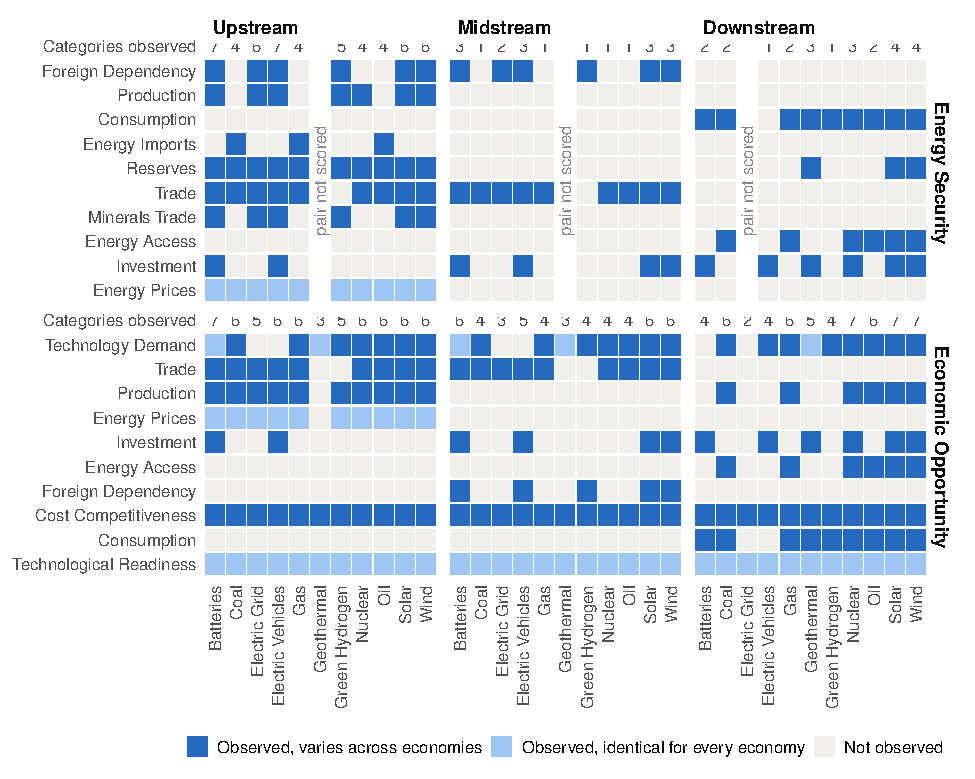
\includegraphics[width=\textwidth]{method_category_sets}
  \caption{Category composition of the pillars by technology--stage pair. Each column is one of
  the 33 headline technology--stage pairs, grouped by stage. Each row is a category of the
  Energy Security pillar (upper block) or the Economic Opportunity pillar (lower block), ordered
  by nominal weight as in Table~\ref{tab:category_weights}. Dark blue: the category is observed
  in the pair and its score varies across economies. Light blue: the category is observed but
  takes the same score for every economy of the pair (a world- or technology-level input).
  Gray: the category is not observed in the pair. The number above each column is the number
  of observed categories, which is the same for every economy of the pair. ``Pair not scored''
  marks the three pairs without an $\ES$ value. Sample: the country--technology--stage cells of
  the eleven headline technologies that have a pillar value (6,232 for $\ES$, 7,131 for $\EO$).
  Source: category contributions in \texttt{data/processed/outputs/index\_outputs.rds};
  \texttt{scripts/paper/fig\_method.R}.}
  \label{fig:method_category_sets}
\end{figure}

\paragraph{Effective weights and constant inputs.} Averaging effective weights over cells instead
of pairs changes the stage means by at most 0.032, because the category set is common within a
pair; the largest gap between effective and nominal share is 0.49. Upstream $\ES$ weight is spread
more evenly, led by Reserves (0.20), Trade (0.18) and Production (0.18); Energy Prices, nominally
0.048, carries 0.10. In $\EO$ the redistribution favours categories observed at every stage:
Technology Demand (0.20 to 0.25, nominal 0.133), Cost Competitiveness (0.19 to 0.24, nominal 0.100)
and Technological Readiness (0.12 to 0.16, nominal 0.067). Categories constant within the pair take
a mean of 0.34 of the weight of an upstream $\EO$ cell, 0.22 at the midstream stage and 0.18
downstream; adding the constant components inside varying categories (world export concentration in
Trade; the addressable-market, global-demand and overcapacity terms of Technology Demand) raises
these shares to 0.46, 0.39 and 0.27. The corresponding component-level shares in $\ES$ are 0.16,
0.20 and 0, the midstream figure being the world export-concentration term of Trade. Energy Prices
is copied to every economy before ranking, so the economies of a technology form one block of tied
ranks: with $T$ technologies the technology in position $p$ receives a percent rank close to
$(p-\tfrac12)/T$ rather than $(p-1)/(T-1)$, and no technology scores exactly 0 or 1.

\paragraph{Imputation burden by category.} Table~\ref{tab:method_imputation} gives the values
behind Figure~\ref{fig:method_imputation}. Upstream, Reserves (0.84) alone accounts for 0.17 of the
$\ES$ stage mean of 0.41; Energy Imports (0.55), Foreign Dependency (0.50) and Production (0.43)
also cover only part of the grid, and the upstream Trade category is imputed at 0.19. In $\EO$,
Technology Demand is imputed at 0.73 to 0.86 and contributes 0.16 to 0.19 to each stage mean: the
addressable-market term counts as imputed for every economy but the United States, the regional
outlook is observed for a median of 12 economies per pair, and the world-level global-demand series
is recorded for 108 economies and filled with the same value for the rest. Investment is imputed at
0.64 to 0.83 in both pillars. World-level series show almost no imputation (Energy Prices below
0.01, Technological Readiness at most 0.04), which is why $\iota_{its}$ records how a value was
obtained rather than whether it is country-specific, and why the rankability rule can admit a cell
whose observed weight is largely world-level. A component averaged across two themes counts as
imputed if either value was, so $\iota_{its}$ is an upper bound there. At the other extreme, 2,055
$\ES$ cells (33 percent) and 407 $\EO$ cells (6 percent) contain no imputed component. Rebuilding
$\iota_{its}$ from the variable table reproduces the builders' value to within $1.1\times10^{-16}$.

% Generated by scripts/paper/fig_method.R; do not edit by hand.
\begin{table}[tbp]
  \centering
  \small
  \begin{threeparttable}
    \caption{Mean imputed share by category, stage and pillar, headline technologies}\label{tab:method_imputation}
    \begin{tabular}{@{}l *{6}{S[table-format=1.2]}@{}}
      \toprule
      & \multicolumn{3}{c}{Energy Security} & \multicolumn{3}{c@{}}{Economic Opportunity}\\
      \cmidrule(lr){2-4}\cmidrule(l){5-7}
      {Category} & {Up} & {Mid} & {Down} & {Up} & {Mid} & {Down} \\
      \midrule
      Consumption & {--} & {--} & 0.03 & {--} & {--} & 0.05 \\
      Cost Competitiveness & {n.a.} & {n.a.} & {n.a.} & 0.34 & 0.42 & 0.36 \\
      Energy Access & {--} & {--} & 0.65 & {--} & {--} & 0.66 \\
      Energy Imports & 0.55 & {--} & {--} & {n.a.} & {n.a.} & {n.a.} \\
      Energy Prices & 0.01 & {--} & {--} & 0.01 & {--} & {--} \\
      Foreign Dependency & 0.50 & 0.54 & {--} & {--} & 0.79 & {--} \\
      Investment & 0.83 & 0.78 & 0.64 & 0.83 & 0.78 & 0.66 \\
      Minerals Trade & 0.02 & {--} & {--} & {n.a.} & {n.a.} & {n.a.} \\
      Production & 0.43 & {--} & {--} & 0.68 & {--} & 0.55 \\
      Reserves & 0.84 & {--} & 0.10 & {n.a.} & {n.a.} & {n.a.} \\
      Technological Readiness & {n.a.} & {n.a.} & {n.a.} & 0.04 & 0.02 & 0.03 \\
      Technology Demand & {n.a.} & {n.a.} & {n.a.} & 0.86 & 0.73 & 0.83 \\
      Trade & 0.19 & 0.01 & {--} & 0.26 & 0.15 & {--} \\
      \midrule
      Pillar, $\bar\iota$ & 0.41 & 0.23 & 0.27 & 0.41 & 0.44 & 0.43 \\
      Cells & {2,181} & {2,002} & {2,049} & {2,394} & {2,346} & {2,391} \\
      \bottomrule
    \end{tabular}
    \begin{tablenotes}[flushleft]\footnotesize
      \item \emph{Notes:} Category rows give the mean, over the country-technology-stage cells
      of the eleven headline technologies in which the category is observed, of the share of the
      category score carried by imputed components,
      $\sum_v\lambda_{vkits}\1[\tilde x_{itsv}\text{ imputed}]$. The pillar row gives the mean
      over all scored cells of the stage of the imputed weight share $\iota_{its}$ of
      equation~\eqref{eq:imputed_share}. --: category not observed at that stage; n.a.: category
      not part of the pillar. Source: \texttt{data/processed/outputs/index\_outputs.rds}
      (variable contributions and the pillar diagnostics); \texttt{scripts/paper/fig\_method.R}.
    \end{tablenotes}
  \end{threeparttable}
\end{table}


\paragraph{Mass points and pair status.} Economies without country-specific data share one value
within their pair: in five $\EO$ pairs (Electric Grid downstream, Green Hydrogen upstream and
midstream, Geothermal upstream and midstream) 65 to 70 economies sit at a single interior value,
and none of these cells is rankable. Observed zeros create mass points that the rule does not
remove: in $\ES$, 98 of the 109 economies scored in Green Hydrogen midstream share the pair's
minimum (0.256), 95 of them rankable, and in Nuclear upstream 127 of 218 share one value (0.172),
105 of them rankable. Such a tie records a real absence of production or resources but becomes a
uniform, sector-wide need under the security-need reading of the Strategic Index. A pair is
\emph{unscored} if no economy has an observed category, \emph{constant} if at least two are scored
and their range is at most $10^{-12}$, and \emph{ok} otherwise. Over every technology, including
those outside the headline set, all 45 $\ES$ pairs and all 40 $\EO$ pairs are ok; Nuclear upstream,
constant before the uranium data were added, now varies. Electric Grid downstream and Geothermal
upstream and midstream have no observed $\ES$ category.

\paragraph{Rankability in detail.} Table~\ref{tab:method_rankability} gives the counts behind
Figure~\ref{fig:method_rankability}. Counted over sovereign cells only, the rule keeps 74 percent of
$\ES$ and 67 percent of $\EO$ cells. Rankable sovereign cells score higher on average than sovereign
cells over the threshold in every pillar and stage, most markedly in midstream $\ES$ (0.46 against
0.30) and midstream $\EO$ (0.49 against 0.37). The narrowest pairs keep a usable comparison set:
Green Hydrogen midstream keeps 40 rankable $\EO$ cells (19 percent of those scored), and Nuclear
downstream, the narrowest $\ES$ pair, keeps 68. The 17 sovereign states without a rankable $\EO$
cell are Liechtenstein, Monaco, Djibouti, Dominica, Eritrea, Haiti, Kiribati, the Marshall Islands,
Micronesia, Nauru, North Korea, Palau, S\~ao Tom\'e and Pr\'incipe, Somalia, St Kitts and Nevis,
St Vincent and the Grenadines and Tuvalu; their only rankable $\EO$ cells had been upstream, and the
upstream Trade category, whose export-size and comparative-advantage terms are imputed for
economies absent from the Comtrade reporter file, lifted their imputed share just over the
threshold. Taiwan keeps 19 rankable $\ES$ and 18 rankable $\EO$ cells. In the Strategic Index the 29
policy-scored economies that lose every cell are nine territories and special administrative
regions (among them Hong Kong, Macau and the West Bank and Gaza) and 20 sovereign states: the 17
above, Andorra, the Central African Republic and Grenada. The pillars are built before the rule is
applied, so excluding a cell does not change the ranking of the cells that remain.

% Generated by scripts/paper/fig_method.R; do not edit by hand.
\begin{table}[tbp]
  \centering
  \small
  \begin{threeparttable}
    \caption{Rankable cells by pillar and stage, headline technologies}\label{tab:method_rankability}
    \begin{tabular}{@{}l *{4}{r} S[table-format=1.2] r@{}}
      \toprule
      & {Scored} & {Rankable} & \multicolumn{2}{c}{Not rankable} & {Share} & {Economies} \\
      \cmidrule(lr){4-5}
      & {cells} & {cells} & {Territory} & {$\iota_{its}>0.5$} & {rankable} & {ranked} \\
      \midrule
      \multicolumn{7}{@{}l}{\emph{Energy Security}} \\
      \quad Upstream & 2,181 & 1,124 & 231 & 826 & 0.52 & 195 \\
      \quad Midstream & 2,002 & 1,397 & 169 & 436 & 0.70 & 192 \\
      \quad Downstream & 2,049 & 1,642 & 207 & 200 & 0.80 & 193 \\
      \quad All stages & 6,232 & 4,163 & 607 & 1,462 & 0.67 & 195 \\
      \multicolumn{7}{@{}l}{\emph{Economic Opportunity}} \\
      \quad Upstream & 2,394 & 1,681 & 250 & 463 & 0.70 & 178 \\
      \quad Midstream & 2,346 & 1,307 & 221 & 818 & 0.56 & 166 \\
      \quad Downstream & 2,391 & 1,313 & 247 & 831 & 0.55 & 169 \\
      \quad All stages & 7,131 & 4,301 & 718 & 2,112 & 0.60 & 178 \\
      \bottomrule
    \end{tabular}
    \begin{tablenotes}[flushleft]\footnotesize
      \item \emph{Notes:} Country--technology--stage cells of the eleven headline technologies
      with a pillar value. A cell is rankable when the economy is a sovereign state (a Correlates
      of War state-system code) and at most $\tau=0.5$ of its index weight rests on imputed components, $\iota_{its}\le\tau$
      (\texttt{config/rankability.yml}). Reasons are exclusive: a territory is counted as a territory
      whatever its imputed share; the next column counts sovereign cells over the threshold.
      Economies ranked: economies with at least one rankable cell. Source:
      \texttt{data/processed/outputs/index\_outputs.rds}; \texttt{scripts/paper/fig\_method.R}.
    \end{tablenotes}
  \end{threeparttable}
\end{table}


% =============================================================================
% Online Appendix to Section 5 (Energy Security): further results.
% Numbers: paper/results/es.json (scripts/paper/fig_es.R, final rerun of 2026-10-12).
% All statistics over rankable cells (config/rankability.yml) unless stated.
% =============================================================================
\section{Energy Security: further results}\label{oa:es}

\paragraph{Rankability.} The rankability rule keeps 4{,}163 of the 6{,}232 scored cells. It removes
the 607 cells of the 24 territories and 1{,}462 cells of sovereign economies whose score rests
mainly on imputation. Among the rankable cells the mean imputed weight share falls to 0.18
upstream, 0.08 midstream and 0.22 downstream. A pair holds between 68 rankable economies (Nuclear
downstream) and 195 (Nuclear upstream). Within each pair every scored economy observes the same
set of categories. The upstream trade baskets give Trade categories to Electric Vehicles, Wind,
Solar and Nuclear upstream, so nine of the ten upstream pairs carry one; Green Hydrogen upstream is
the exception.

\paragraph{Distribution by pair.} In Electric Grid, Solar and Green Hydrogen upstream the
interquartile range is narrower than 0.05. Upstream pair medians run from 0.17 in nuclear and 0.20
in batteries and electric vehicles to 0.47 in oil. Midstream and downstream the pillar rests mainly
on median-centred S-curves; the four midstream pairs scored on Trade alone (gas, coal, oil and
nuclear) have medians between 0.48 and 0.56. Green Hydrogen midstream, scored on Foreign Dependency
alone, gives 90 per cent of its 106 rankable economies the value 0.26; Green Hydrogen downstream,
scored on Consumption alone, is bimodal (interquartile range 0.10 to 0.72). Within stages,
technology-stage effects explain 33, 50 and 22 per cent of the upstream, midstream and downstream
variance, and country effects 51, 65 and 29 per cent of the within-pair remainder. Subtracting
the contributions of Energy Prices and of the world-concentration terms of Trade and Minerals
Trade leaves the pair-effect $R^2$ at 48 per cent.

\paragraph{Drivers.} Investment, defined midstream only for batteries, electric vehicles, solar and
wind, supplies 1.4 per cent of the midstream score against a mean effective weight of 7.0 per cent,
because the investment monitor records neither manufacturing investment nor capacity for most
economies (72 per cent of rankable economies score zero in the median of these pairs). Downstream,
resource potential supplies 10 per cent and Investment 9.8 per cent against a weight of 19 per
cent. The concentration term of Minerals Trade is constant for all economies except Taiwan and
R\'eunion, which lie outside the World Bank list. Energy Prices scores range from 0.19 for gas to
0.81 for the electric grid, raising every economy's upstream score by between 0.025 (batteries)
and 0.088 (nuclear) without changing any within-pair rank.

\paragraph{Correlation among categories.} The median within-pair Spearman correlation between two
categories is 0.42 upstream (one of 78 pair-specific correlations is negative, $-0.01$), 0.33
midstream and 0.11 downstream. Reserves and Production correlate at a median of 0.84 over the
seven pairs that carry both, and at 0.87 among the economies with a positive score on both (a
median of 16 per pair). Foreign Dependency correlates with Production at 0.76 and with Reserves at
0.69. Midstream, Foreign Dependency and Trade correlate at only 0.28 (range $-0.23$ to 0.48):
economies with large shares of refined supply and manufacturing capacity are not always those with
large export shares and small net imports. Downstream, Energy Access and Consumption correlate at
0.12 and resource potential correlates negatively with Consumption ($-0.11$). Within a pair the
pillar's ranking follows Energy Imports (median Spearman correlation with $\ES_{its}$ of 0.80),
Minerals Trade (0.79) and Reserves (0.79) upstream, Trade (0.94) midstream, and Investment (0.76)
and Consumption (0.74) downstream.

\paragraph{Uranium.} An economy with neither resources nor production scores the Energy Prices
contribution, $0.704/8=0.088$, plus its Trade category. For the 105 economies whose uranium trade is
not observed, Trade is imputed and the score is 0.172 (shared rank 67); the other 32 economies
without uranium score between 0.145 (Trinidad and Tobago) and 0.201 (Norway). Their imputed weight
shares lie between one quarter and one half, so all remain rankable. Producers dominate the top,
though not all of it: T\"urkiye, which holds resources but reports no mine output, ranks 18th
(0.34), and the lowest-ranked producer is 26th. Nine of the 15 highest-ranked economies are
coalition members. Among the 26 members without identified resources are France, the United
Kingdom, South Korea, the Netherlands, Norway and Poland.

\paragraph{Leaders.} China's eleven first places are Batteries, Electric Vehicles and Wind upstream,
where its shares of world mineral supply, production and trade dominate; Batteries, Electric Grid,
Electric Vehicles, Solar and Wind midstream; and Batteries, Nuclear and Wind downstream. South
Africa leads green hydrogen upstream, whose mineral weights are dominated by the platinum-group
metals, and Chile the grid and solar upstream, in which copper carries most of the demand weight;
in Electric Grid upstream, whose basket holds copper and aluminium inputs, the Democratic Republic
of the Congo and Peru follow Chile. The midstream pairs scored on Trade alone are led by Poland
(coal), South Korea (gas and oil) and Russia (nuclear, whose basket holds enriched uranium, reactor
components and steam-cycle equipment). Indonesia leads Green Hydrogen midstream, in which 95 of
106 rankable economies share one value. Downstream, Qatar leads oil, Kuwait gas, Indonesia coal,
Saudi Arabia solar, the United States geothermal and green hydrogen, and T\"urkiye electric
vehicles, a pair that rests on Investment alone.

In Oil upstream (Figure~\ref{fig:es_top}) Saudi Arabia leads (0.81); the United States is 12th
(0.71) and China 34th (0.55). The cell-constant inputs give every economy 0.16; of the gap between
the top-ten mean and the pair mean, Reserves accounts for 58 per cent, Energy Imports for 28 and
the country-varying part of Trade for 13. China's Reserves and Trade scores (0.64 and 0.79) are
close to those of the United States (0.69 and 0.87), but its Energy Imports score is 0.25 against
0.68. In Batteries and Solar midstream China leads with 0.77 (United States 0.56) and 0.82 (India
0.67), and coalition members fill the other nine top-ten places of each, among them Indonesia and
Malaysia in batteries and Thailand, Malaysia, Viet Nam and Indonesia in solar. Investment accounts
for 62 and 58 per cent of the top-ten gap in these pairs (mean scores 0.13 and 0.09, top ten 0.61
and 0.58); China's lead over the runner-up comes from Foreign Dependency (0.37 against 0.21 in
batteries, 0.40 against 0.28 in solar), while on Investment the United States scores higher than
China in batteries (0.86 against 0.80).

\paragraph{The coalition's tiers.} The partners, several of which enter as major suppliers, have the
higher upstream mean percentile (0.63 against 0.56 for the core), while the core is ahead midstream
(0.78 against 0.64) and downstream (0.64 against 0.59). The 21 EU members of the coalition are
weaker upstream than the other members (0.50 against 0.64) and stronger midstream (0.79 against
0.67). By mean within-pair percentile the United States (0.95), Canada (0.89), Australia (0.82),
India (0.79) and Poland (0.77) lead, and Qatar (0.44), Ghana (0.45), Gabon (0.46), Namibia (0.46)
and Luxembourg (0.47) trail. Midstream, Japan has the highest mean percentile of any member (0.95),
ahead of Germany, the United States, India and South Korea. Of the 1{,}710 member cells in the 30
scored pairs, 1{,}606 are rankable, 96 scored but not rankable and 8 unscored; the non-rankable
cells concentrate in Namibia, Costa Rica, the Dominican Republic, Guatemala and Ghana (rankable in
13 to 15 of their 28 or 29 scored pairs) and Canada (23 of 29).

\paragraph{The United States, China and Taiwan.} The United States leads two pairs (Geothermal and
Green Hydrogen downstream); its weakest positions are 30th in Nuclear midstream, 23rd in Oil
downstream, 22nd in Electric Grid midstream and 17th in Nuclear downstream. China is in the top ten
of every midstream pair. Its weak positions are those of a fossil-fuel importer (33rd in gas and
34th in oil upstream, 24th in gas downstream) and two downstream pairs in which deployment data
place it low: 63rd in green hydrogen and last of 186 in oil, where Consumption carries five-ninths
of the weight and no rankable economy has lower projected growth of oil-fired capacity. The United
States ranks above China in 8 of the 30 pairs, all upstream or downstream fossil-fuel and resource
pairs and none midstream. Taiwan, scored in 28 cells and rankable in 19, has a midstream mean
percentile of 0.75 (ranks 27th to 61st on Trade) and 0.01 across its seven rankable upstream pairs,
with no place in any top ten.

\paragraph{Ties.} In Green Hydrogen midstream the United States' rank of 12 is shared with 94 other
economies, and in Green Hydrogen downstream 49 economies share third place at 0.72.

% =============================================================================
% Online Appendix to Section 6 (Economic Opportunity): construction details and further results.
% Numbers: paper/results/eo.json (scripts/paper/fig_eo.R) and eo_transforms.json
% (scripts/paper/fig_eo_transforms.R), final rerun of 2026-10-12. Statistics over rankable cells
% (config/rankability.yml) unless stated.
% =============================================================================
\section{Economic Opportunity: construction details and further results}\label{oa:eo}

\subsection{Construction details}

\paragraph{Trade.} Revealed comparative advantage complements market share: a small economy can be
highly specialised in a basket without a large share of the world market, and specialisation is
what the complexity literature reads as revealed capability. Basket export value is a second
measure of scale from a source with different coverage and year. Feasibility is the forward-looking
element: a country with no exports of a basket can score well if it exports products that require
similar capabilities. An economy that does not report to Comtrade is scored on its two Atlas
components and the world-market term. The net-import term of the ES category is not used in EO.

\paragraph{Production.} Absolute growth rewards large producers whose output expands by the most
units, relative growth rewards fast growth from a small base, and the composite balances the two;
level and change each enter the category twice, directly and through the composite. In the mineral
block, tonnes of different minerals cannot be added, so each mineral enters as a share of world
supply weighted by the technology's share of the mineral's demand; the horizon level is divided by
base-year world supply, so the change is a change in quantity, not in market share. A country the
IEA supply table does not name for a mineral counts as zero there. Uranium mine output from the Red
Book is scored like oil, gas and coal.

\paragraph{Technology Demand.} Growth in the World Energy Outlook composite is absolute because a
relative measure ranked across fuels would put hydrogen's near-zero base at the top; the value is a
property of the technology, the same at every stage and for every economy. The BCG addressable
market is ranked across the 26 cells it sizes and copied to every economy by the global-average
rule. Coverage is uneven: the electric grid has no input in any source and so no Technology Demand
category, electric vehicles have it only downstream, downstream batteries lack it because BCG does
not size that cell, and geothermal is scored on the BCG entry alone.

\paragraph{Technological Readiness.} The bell rises over four steps and falls over five, so an
item at TRL 9 keeps a level score of $\cos(3\pi/10)\approx0.59$ and one at TRL 3 scores
$\cos(3\pi/8)\approx0.38$; the concave momentum term gives the first step of progress the largest
increment. Of the 253 mapped items, 9 map to more than one cell; 98 carry a post-TRL-9 adoption
stage, 43 per cent sit at TRL 9 or above, and the 26 items that are commercial in many markets score
zero on level. Of the items with a 2020 reading, 54 per cent did not move. Ten of the 33 headline
cells take their technology's value because no item maps to the stage; the index differs across the
three stages of ten of the eleven technologies (wind keeps one value), with a median range across a
technology's stages of 0.16. The parameters (bounds 2 and 11, peak 6, momentum weight 0.3, cap of
three steps, exponent 1/2) are the theme builder's defaults.

\paragraph{Overcapacity.} Of the four midstream technologies the BloombergNEF supply-chain data
cover, solar ($\rho=2.3$, index 0.20), batteries and wind ($\rho=3.0$, 0.13 each) sit on the steep
part of the curve, and green hydrogen ($\rho=18.2$) is effectively at zero.

\paragraph{Cost Competitiveness.} Wages are converted at market exchange rates rather than
purchasing-power parities because the price-level difference that PPP conversion removes is the
cost advantage being measured. The lending rate is winsorised at its 5th and 95th cross-country
percentiles before min-max rescaling; producer-price inflation enters as a rate because each
country's price index has its own base year. Stale observations and gaps are filled from regional
and income-group peers. The Input Cost Index carries the category wherever the LCOE and equipment
cost components are absent and half of it where one is present; counting each source once avoids
giving BNEF three of four votes wherever it covers a market.

\subsection{Further results}

\paragraph{Rankability.} Of the 2{,}830 cells the rule sets aside, 2{,}112 carry more than half of
their weight on imputed components, 74 belong to territories and 644 fail on both counts. The rule
bites hardest where country-specific sources are thinnest: 70.2 per cent of upstream cells are
rankable, against 55.7 per cent midstream and 54.9 per cent downstream. In Batteries midstream 42
of the 54 rankable economies have an observed Foreign Dependency or Investment input, in Green
Hydrogen midstream 30 of 40. The mean imputed weight share of rankable cells is 0.29. Ranked among
all scored economies of their pair, cells excluded for imputation alone have a mean percentile of
0.43 (63.4 per cent below the median) and territory cells 0.42, against 0.55 for rankable cells.
Both decompositions reconcile exactly (largest gaps 0 and $1.1\times10^{-16}$); 45.3 per cent of
category scores contain an imputed component.

\paragraph{Distribution.} Over all scored cells the midstream median is 0.454 and its lower
quartile 0.328, because the zero rule places economies without recorded capacity or investment at
the bottom of the clean-technology midstream pairs, and the rule removes most of them. Four of the
five clean-technology midstream pairs (wind, electric vehicles, solar, batteries) have the lowest
midstream medians (0.351 to 0.426). The widest boxes owe their width to one category each: in EV
midstream (interquartile range 0.144) Foreign Dependency, observed for 97 of 145 rankable
economies, accounts for 46 per cent of the variance (0.053 without it); in Green Hydrogen
downstream (0.122) Consumption accounts for 94 per cent; in Wind downstream (0.117) Investment
accounts for 46 per cent.

\paragraph{Variance and persistence.} Technology effects alone explain 27.8 per cent of the
variance and stage effects almost nothing (0.01 per cent), so a pair's level is set by its
composition rather than its stage. Over all scored cells the pair share is 71.5 per cent. Across
the 159 economies rankable at all three stages, the Spearman correlation of mean within-pair
percentiles is 0.86 between upstream and midstream, 0.70 between upstream and downstream and 0.79
between midstream and downstream. Part of this common factor is the Input Cost Index, a
country-level index whose stage variation comes only from the wage activity and the factor shares:
across the 178 economies with a rankable cell, mean EO percentile and mean Cost Competitiveness
percentile correlate at 0.77 (0.82 across the 57 coalition members).

\paragraph{Drivers.} Level shares: upstream Cost Competitiveness 21.9 per cent, Technology Demand
17.3, Production 16.5 and Energy Prices 16.2; midstream Cost Competitiveness 29.2, Technology Demand
24.7 and Trade 24.6; downstream Cost Competitiveness 27.5, Technology Demand 19.7 and Technological
Readiness 18.0. Within-pair variance shares: upstream Trade 26.9 and Production 22.4; midstream
Trade 25.5 and Foreign Dependency 22.2; downstream Consumption 23.8 and Investment 22.2. Investment
contributes 0.3, 1.2 and 4.2 per cent of the level by stage but 8.3, 12.7 and 22.2 per cent of the
within-pair variance, because under the zero rule the few economies with recorded investment stand
far above the majority without it (in 9 of the 12 pairs that carry the category). The upstream
constants are led by price volatility (15.9 per cent of effective weight), the TRL Index (12.5) and
the addressable market (10.1). Before the rankability rule the observed country-specific share is
32.3 per cent and the imputed share 30.1 per cent.

\paragraph{Leaders.} Chad combines low recorded wages with a 2017 lending rate of 2.45 per cent, the
joint fifth lowest of the 144 rates in the cost theme; the runner-up in its three pairs is Cameroon,
with the same rate (2018), and Chad's margins are 0.0020, 0.0005 and 0.0011. Canada leads nuclear
upstream (0.65) and China electric-grid upstream (0.71, ahead of Chile at 0.65), the pair built on
the copper and aluminium basket. The leader's margin is below 0.01 in seven pairs; the United States
has the largest non-Chinese margin (0.153 over Indonesia in geothermal downstream). Coalition
members hold 69.1 per cent of the 330 top-ten places; China is in the top ten of 30 pairs and the
United States of 20. The United States ranks in the bottom half of one pair only, 109th of 141 in
electric-grid downstream, a cost-only pair; in the mineral-based upstream pairs it ranks between
third (wind) and 62nd (green hydrogen). China's one low rank, 98th of 104 in oil downstream, comes
from Consumption and the growth component of Production.

\paragraph{The coalition.} Among core members the United States (0.89), Portugal (0.84), Poland
(0.84), the Czech Republic (0.81) and Spain (0.80) rank highest and the United Kingdom (0.57),
Romania (0.52), Australia (0.46), New Zealand (0.34) and Ukraine (0.11) lowest; among partners,
Thailand (0.82), Indonesia (0.80), Malaysia (0.79), India (0.78) and Saudi Arabia (0.66) rank highest
and the Dominican Republic (0.26), Brazil (0.23), Argentina (0.19), the Democratic Republic of the
Congo (0.13) and Ghana (0.10) lowest. T\"urkiye, Brazil, Argentina and Ghana record nominal lending
rates of 39.0, 46.0, 59.7 and 27.0 per cent, at the winsorisation ceiling; with the Cost
Competitiveness contribution set to its pair mean their mean percentiles would be 0.73, 0.61, 0.45
and 0.39 rather than 0.30, 0.23, 0.19 and 0.10, and Ukraine's (rate 18.9 per cent) 0.50 rather than
0.11; six members gain more than 0.2. At the top the same change would lower Portugal from 0.84 to
0.62, Thailand from 0.82 to 0.64 and Ireland from 0.71 to 0.51, while the United States barely
moves. The BNEF regional composite of Technology Demand is observed for at most twelve economies
and the global-average rule gives the others their mean, so a modelled economy below that mean
ranks below many unmodelled ones: Australia's value is below the mean in all 18 pairs in which it is
observed, the United Kingdom's in 14 of 18 and France's in 15 of 21; with Technology Demand at its
pair mean their mean percentiles would be 0.52, 0.65 and 0.80 rather than 0.46, 0.57 and 0.76.

Of the core members' 1{,}023 scored cells 1{,}002 are rankable, against 716 of the partners' 858.
Gabon has only 9 rankable cells, Oman 21, Saudi Arabia and Singapore 22 each, and Morocco, Namibia
and Costa Rica 23. The mean imputed weight share of rankable cells is 0.20 for the core, 0.27 for
the partners, 0.33 for other economies and zero for the United States, partly because the BCG
addressable market is recorded for the United States alone. Within pairs the median Spearman
correlation between $\EO_{its}$ and the imputed share is $-0.28$.

\paragraph{Illustrative pairs.} Oil upstream is led by the United States (0.659), China (0.644),
Canada (0.637), Saudi Arabia (0.622) and Norway (0.607); Saudi Arabia, Iraq, Iran, Kuwait and the
United Arab Emirates share the smallest Cost Competitiveness contribution (0.095, an imputed value)
and owe their places to production and trade. In Batteries midstream China (0.771) leads the United
States (0.633) on Foreign Dependency (0.167 against 0.106) and Cost Competitiveness (0.142 against
0.073), while the United States' Investment contribution (0.143) exceeds China's (0.134); nine of
the ten are coalition members. In Solar midstream China (0.788) is followed by India (0.640) and
the United States (0.635), then Viet Nam, Thailand, Indonesia, Malaysia and the Philippines, with
France and Germany eighth and ninth. In EV downstream emerging economies take eight of the ten
places: China (0.755), Viet Nam (0.731), Thailand (0.705) and T\"urkiye (0.702) lead, because the
EV-market composite, half of whose indices are growth rates (equation~\eqref{eq:eo_ev}), rewards
markets growing fast from a small base; T\"urkiye, Viet Nam and the Philippines receive larger
Technology Demand contributions than China.

% =============================================================================
% Online Appendix to Section 7 (the opportunity-security space): further results and caveats.
% Numbers: paper/results/joint.json (scripts/paper/fig_joint.R, final rerun of 2026-10-12).
% Sample: cells rankable on both pillars (config/rankability.yml).
% =============================================================================
\section{The opportunity-security space: further results}\label{oa:joint}

\paragraph{Sample.} Of the 3{,}075 cells scored by both pillars but not rankable on both, 607
belong to territories and 2{,}468 to sovereign economies whose imputed weight share exceeds one
half in Energy Security only (721), in Economic Opportunity only (1{,}006) or in both (741). The
number of rankable economies per pair ranges from 40 (Green Hydrogen midstream) to 175 (Nuclear
upstream). In this sample technology-stage fixed effects account for 41.9 per cent of the variance
of $\ES_{its}$ and 53.4 per cent of that of $\EO_{its}$. The six EU members that enter the allied
network only through the EU node are not counted as coalition members.

\paragraph{Co-movement by technology.} The within-pair correlation exceeds 0.5 in 19 of the 30
pairs and is negative only in Green Hydrogen midstream. Pooled on levels it is 0.48 and on pooled
within-pair ranks 0.57. The stage gradient holds within wind (0.37, 0.72 and 0.89 by stage),
nuclear (0.16, 0.49, 0.89), coal (0.35, 0.56, 0.79), gas (0.40, 0.54, 0.78) and oil (0.50, 0.55,
0.75). Solar (0.48, 0.78, 0.58) and electric vehicles (0.60, 0.94, 0.80) peak midstream; in
batteries the correlation falls along the chain (0.63, 0.61, 0.40); in green hydrogen the midstream
value ($-0.21$) lies below the upstream one (0.03). Medians by technology run from 0.03 (green
hydrogen) to 0.80 (electric vehicles). Upstream the correlation is positive in all ten pairs. In the
five mineral pairs with a trade basket on both sides (batteries 0.63, grid 0.60, electric vehicles
0.60, solar 0.48, wind 0.37), opportunity's Trade and security's Minerals Trade measure exports of
overlapping materials and correlate at 0.70 to 0.85. The fossil-fuel pairs follow (oil 0.50, gas
0.40, coal 0.35); nuclear (0.16) has half of its economies at one security value, and green
hydrogen (0.03), the only upstream pair without a trade basket, rests on platinum-group endowments
on the security side and on cost, demand, readiness and production on the opportunity side.

\paragraph{Shared components.} A component counts as shared when the other pillar contains a
component of the same category with identical observed values: every component of Consumption,
Energy Access, Investment and Energy Prices, two of the three security and two of the five
opportunity components of Trade, and five of the six components of Foreign Dependency in each
pillar; no Production component. In seven downstream pairs (batteries, coal, electric vehicles,
gas, green hydrogen, nuclear, oil) the security score is a reweighting of part of the opportunity
score, which is why Green Hydrogen (0.92) and Nuclear (0.89) downstream show some of the highest
correlations. The non-shared median correlation has an interquartile range of 0.20 to 0.40, a 45
per cent reduction from the full pillars. The level covariance is positive in all 30 pairs,
including Green Hydrogen midstream. Of the pooled within-pair covariance, the two cross terms of
equation~\eqref{eq:joint_cov} account for 24 per cent and the non-shared term for 16 per cent
(58 per cent upstream, nothing downstream); in the median pair the shared term accounts for 19 per
cent. The cross terms are not definitional but run through shared inputs.

The non-shared rank correlation is 0.37 midstream and 0.30 upstream. The pillars' distinctive trade
components (net imports and, upstream, minerals trade for security; revealed comparative advantage,
export size and feasibility for opportunity) all reward exporters of the stage's basket; removing
opportunity's trade components as well lowers the medians to 0.15 midstream and 0.02 upstream. In
the three downstream pairs where it can be computed (geothermal, solar, wind) it is $-0.04$.

\paragraph{Category correlations.} Consumption, Energy Access and Investment correlate perfectly
with their counterparts; Trade, sharing two components, 0.62; Production, from different sources
and transformations of the same physical quantity, 0.27; and Foreign Dependency, whose shared
components are missing for many economies and imputed under different rules, 0.04. The median
correlation between categories with different names is 0.14 over 47 category pairs. Technology
Demand and Cost Competitiveness have absolute correlations of at most 0.12 and 0.17 with every
security category (the most negative is Cost Competitiveness with Reserves, $-0.17$). Within
security, Production and Reserves average 0.79 across seven upstream pairs (0.72 to 0.91 in the six
critical-mineral pairs, where 62 to 85 per cent of rankable economies record zero on both); Nuclear
upstream has the lowest value (0.61), because many holders of uranium resources do not mine them.

\paragraph{Regions.} Laggards outnumber leaders because a tied cell at a median counts as low and
ties are common where a pillar rests on a zero-anchored component. Across pairs, the observed share
of opportunity without security tracks the copula-implied one (correlation 0.90). Off-diagonal
shares are 19.5 and 17.2 per cent upstream, 13.8 per cent (opportunity without security)
midstream, and 12.4 and 10.2 per cent downstream; by technology the leapfrog share runs from 9.5
per cent (electric vehicles) to 20.2 per cent (green hydrogen and nuclear). In Green Hydrogen
midstream 34 of 40 economies share the lowest security value, which is also the median; in Nuclear
upstream 87 of 175 share 0.172, the median, and 37 of the 49 cells in the leapfrog region are such
economies. Counting ties as high empties the region in Green Hydrogen midstream and lowers it to
6.9 per cent in Nuclear upstream. The next pairs, Green Hydrogen upstream (24 per cent), Coal
upstream (22) and Batteries downstream (21), have few ties and shares near the copula value.

\paragraph{The coalition.} The partners, many of them major suppliers, have 21.4 per cent of cells
with security but not opportunity. The median core member has 16.7 per cent of its pairs in the
leapfrog region, the median partner 6.9 per cent. Austria, Portugal, Luxembourg (11 of 30 each),
Ireland (10) and Croatia (9) lead; without the two tie pairs their counts are 9, 10, 10, 8 and 7.
Among partners the largest counts are Thailand and the Philippines (5 of 29), then Malaysia, Viet
Nam and Qatar (4). Thirteen members have no leapfrog pair: Canada, Japan, the United Kingdom,
Australia and Ukraine in the core, and T\"urkiye, Brazil, Argentina, the Democratic Republic of the
Congo, the Dominican Republic, Gabon, Namibia and Ghana among partners. Brazil, a partner on its
reserves alone, is the clearest case of security without opportunity. The pairs most often in the
leapfrog region across members are Gas and Oil upstream and Green Hydrogen midstream (14 members
each), Coal upstream (13), Solar downstream (12), Nuclear upstream (11) and Grid upstream (10);
without the two tie pairs the coalition share falls from 12.8 to 11.8 per cent. Members' rankable
pairs number 22 to 30 in the core and 9 to 29 among partners, so the shares of Costa Rica, Gabon,
Namibia (9 pairs), Guatemala (10), the Dominican Republic and Ghana (11) rest on few cells.

\paragraph{Within countries.} Of the 174 countries with a Strategic Index, seven with fewer than
five cells are left out; the remaining 167 have 5 to 30 cells (median 22; 50 have fewer than ten).
The correlation is positive for 164 countries; the three exceptions (Afghanistan, Bhutan, the
Maldives) are not members. Among members it averages 0.52, from 0.27 (New Zealand) to 0.77 (Viet
Nam). Security varies more than opportunity across a country's sectors (mean standard deviations
0.15 and 0.07); the covariance share ranges from 16.5 per cent (Ghana) to 66 per cent (India) among
members, and the standard deviation of $\Delta_{its}$ from 0.068 (Lao PDR) to 0.26 (the Gambia).
The pairs' mean pillar values are only weakly related across pairs (0.33); after subtracting pair
means the within-country correlation rises to 0.67 and the standard deviation of the gap falls to
0.08, so part of the gap's spread is common to every country.

\paragraph{The Strategic Index and the regions.} Every Strategic Index cell (3{,}154 for 174
countries) lies in this sample. A country's top sector, before eligibility rules, lies in the
leapfrog region for 47 of 174 countries (27.0 per cent; 15 members), against 15.2 per cent of
cells. Nuclear upstream is the top sector of 62 countries, 43 of them at the common security value,
which gives a large need whichever side of the opportunity median they fall. After the endowment
screen, 169 countries keep an eligible cell and for 35 of them (20.7 per cent) the top one lies in
the region. Of the 57 allied picks (43 midstream), the eight in the region are Austria, Belgium,
Italy, the Netherlands, Romania and Viet Nam in Batteries midstream and Indonesia and Slovakia in
Nuclear midstream; 21 are leaders, 14 have security without opportunity and 14 are laggards, while
61.0 per cent of eligible sectors are leaders. None of the eight Nuclear upstream picks is in the
region: all eight members hold or mine uranium. Costa Rica, the Dominican Republic and Guatemala have
four eligible sectors each (nuclear, oil, gas and coal midstream) and Namibia five (the same and
Nuclear upstream). Midstream nuclear security is built from Trade alone and compressed around its
median (quartiles 0.435, 0.482, 0.530), so their security ranks of 0.50 to 0.71 lie at or above it,
and the technology weight (nuclear 0.999, gas 0.422, coal 0.024, oil zero) favours nuclear.

\paragraph{Caveats.} Percentile ranks discard distances, and the median split turns small
differences into differences of region; where many economies tie at a median the convention
decides the region of the whole group (counting ties as high lowers the upstream leapfrog share
from 19.5 to 15.5 per cent and the coalition's from 12.8 to 10.8). Regions are relative to the
rankable economies of each pair, a set that leans towards economies with good statistical
coverage. The rank-based measure of mechanical overlap covers 23 pairs; the covariance decomposition
covers all 30 but concerns levels and is dominated by the pairs with the largest covariances.
Within-country statistics compare category bundles that differ across pairs. The endowment screen
is a rule for the allied picks, not part of either pillar or of the index. More generally, shared
components make the implied trade-offs of a composite hard to see in the aggregate
\citep{ravallion2012mashup}; inspecting the correlation structure among indicators
\citep{oecd2008handbook} is what reveals them here.

% Online Appendix to Section 7.5 (sec:coalition). Numbers: paper/results/coalition.json.
\section{Coalition rule: data and further results}\label{oa:coalition}

\paragraph{Supply and reserves measures of the supplier route.} An economy passes the supplier test
if, in at least one Upstream or Midstream stage of a headline technology, it holds at least 5
percent of the world total of one of the following supply measures, or at least 10 percent of world
reserves of a resource the stage extracts. Supply: exports of the stage's HS6 basket
\citep[2023;][]{growthlab2019trade}; oil, gas and coal production \citep[2025;][]{ei2026statistical};
uranium mine production (2024, \citealp{oecdnea2026uranium}); mine production and refining of the
minerals a technology uses \citep[2025;][with manganese, zinc and platinum-group metals from the
Energy Institute]{iea2026cmdata}; and clean-technology manufacturing capacity (2024). Reserves: the
critical-mineral reserves of \citet{usgs2026mcs} at the end of 2025 (cobalt, lithium, graphite, rare
earths, copper, manganese, nickel, zinc and platinum-group metals; the report's erratum puts Brazil's
rare earths at 11 Mt), proved oil, gas and coal reserves at the end of 2020 \citep{ei2026statistical}
and identified uranium resources recoverable below USD 260/kgU \citep{oecdnea2026uranium}. Holders
whose reserves USGS does not quantify (entries NA, W or s) count as zero, so world shares are
measured on quantified holdings. The route reads the same reserves tables as the Reserves category
of the Energy Security pillar (Section~\ref{sec:es}). The 10 percent bar binds for a small group:
six economies that are not China-leaning hold between 5 and 10 percent of a world reserve without
otherwise qualifying (Madagascar 8.7 percent of graphite, Mozambique 8.1 percent, Kuwait 5.9 percent
of oil, Tanzania 5.8 percent, Niger 5.7 percent of uranium, New Caledonia 5.1 percent of nickel), as
do Iraq, Turkmenistan and the United Arab Emirates, which are China-leaning.

\paragraph{GDP floor.} The floor of USD 100 billion (current dollars, latest year, 2025 for every
member) excludes 18 U.S.-leaning economies, among them six EU members and small European and Pacific
states, and 16 members of the five agreements, the largest Lithuania (USD 95 billion), which enters
through the EU node, and Panama (USD 91 billion). Puerto Rico inherits the U.S. position and exceeds
the floor but has no vote of its own and is not a member.

\paragraph{Supply cover of the coalition.} Across the 18 Upstream and Midstream stages with an HS6
basket, the 63 economies of the coalition (the 57 members and the six EU members below the GDP floor) account for a median 70.7 percent of world exports, from
45.2 percent in Wind Upstream to 88.4 percent in Batteries Upstream, and China for a median 17.6
percent, with a maximum of 40.9 percent in Batteries Midstream. The coalition's share exceeds China's
in all 18 stages, but in two Upstream stages the excluded China-leaning suppliers other than China
hold large shares: 31.3 percent of Wind Upstream exports (coalition 45.2) and 47.6 percent of Nuclear
Upstream exports (coalition 50.0). Coalition economies mine 81.9 percent of the world's cobalt, 79.4
percent of its nickel, 60.0 percent of its lithium and 54.5 percent of its copper, but 3.6 percent of
its graphite and 14.3 percent of its rare earths; they refine 17.4 percent of cobalt, 23.2 percent of
copper, 24.6 percent of lithium, 5.5 percent of graphite and 12.6 percent of rare earths, against
China's 75.6, 46.8, 73.7, 94.4 and 83.9 percent; nickel refining is 55.7 percent in the coalition.
Coalition economies hold 75.8 percent of quantified world cobalt reserves, 77.3 percent of lithium,
85.5 percent of manganese, 78.8 percent of nickel and 83.9 percent of platinum-group metals, but 33.3
percent of rare earths (China 58.4) and 35.7 percent of graphite (China 32.3). In oil and gas the
excluded China-leaning suppliers other than China hold about as much as the coalition or more (35.3
against 35.7 percent of oil reserves, 43.4 against 30.8 percent of gas).

\paragraph{Dyadic alignment among members.} Counting EU members individually, the 1,596 pairs of
members split 29.3, 64.8 and 5.8 percent across $A_{ij}=1$, $\tfrac12$ and 0. The three China-leaning
partners have $A_{ij}=0$ with every core member and $A_{ij}=1$ with China and Russia.

\paragraph{Sensitivity of the blocs.} With session 78 alone (192 economies; Spearman 0.966 with the
headline, 89.1 percent in the same bloc), New Zealand falls just
below the U.S.-leaning cut ($s=0.583$ against 0.584) and becomes a partner through IPEF, Saudi Arabia
becomes China-leaning and loses its supplier route, Myanmar becomes nonaligned and enters as a
supplier, and India becomes China-leaning but remains a partner through IPEF and the MSP. With the
final-passage series (sessions 76--80, 193 economies, 89.6 percent in the same bloc) the cuts move to
0.446 and 0.055: China-leaning economies cluster more tightly around China in final-passage votes,
and Russia ($s=0.117$), Kazakhstan (0.056) and Myanmar (0.163) would enter the coalition as major
suppliers; Malaysia becomes China-leaning but stays through IPEF.

\paragraph{The earlier hand-picked list.} Of the 23 members fixed by hand in an earlier version, the
United States, Canada, Japan, Australia, Korea, the United Kingdom, Germany, France, Italy, Norway and
Denmark are core members, and India, Mexico, Brazil, Saudi Arabia, South Africa, Indonesia, Viet Nam,
Argentina, Morocco and Chile are partners. The United Arab Emirates (largest supply share 4.2
percent, oil reserves 5.6 percent) and Kenya leave. The 16 new partners are Colombia, Costa Rica, the
Democratic Republic of the Congo, the Dominican Republic, Gabon, Ghana, Guatemala, Malaysia, Namibia,
Oman, Peru, the Philippines, Qatar, Singapore, Thailand and T\"urkiye.

% Online Appendix to Section 8 (sec:strategic). Numbers: paper/results/strategic.json and
% si_fixed_inputs.json (final rerun of 2026-10-12). Specification: R/categories/policy/
% iea_policy_index.R, cat_policy_index.R, R/indices/build_policy_index.R, R/indices/build_indices.R.
\section{The Policy index and the Strategic Index: further detail}\label{oa:strategic}

\paragraph{Tagging and strength of IEA policies.} Each policy of the IEA Policies and Measures
database \citep{iea2026pams} is assigned to technologies first from its own technology list and,
failing that, from keyword rules applied to its title and text; a policy matched to no technology
is cross-cutting and counted in every technology. Stages are assigned by keyword rules on the text:
Upstream on whole words for mining, mines, exploration, extraction, ores, leases, concessions and
drilling; Midstream on processing, refining, smelting, manufacturing, factories, plants, components,
supply chains and domestic content; Downstream on deployment, installation, consumers, end use,
adoption, efficiency, demand, charging, grid connection, power plants and generation. A policy that
matches no stage is cross-cutting across the three. Its strength is
$\sigma_h=w_{\mathrm{type}}\,w_{\mathrm{status}}\,w_{\mathrm{juris}}\,w_{\mathrm{tech}}\,w_{\mathrm{stage}}$
with type weights 0.85 (financial incentives), 0.70 (public procurement), 0.50 (regulations and
standards; research, development and demonstration), 0.20 (information and labelling; other) and
0.10 (voluntary and coordination measures); status weights 1 (in force), 0.60 (planned), 0.50
(proposed), 0.20 (expired or unknown) and 0 (ended); jurisdiction weights 1 (national), 0.66
(international), 0.50 (subnational, state, provincial or regional), 0.30 (unknown) and 0.25 (local);
a technology discount of 0.70 for a cross-cutting policy and 0.30 for a technology found only in the
text; and a stage discount of 0.75 for a cross-cutting stage. A policy counted in several cells
carries its full strength in each. Upstream words are matched as whole words, because as substrings
``ore'' and ``mine'' match ``more'', ``Korea'' and ``determine''.

\paragraph{The Climate Action Tracker component.} The Tracker rates 65 economies in the final build:
39 in their own right and 26 EU members through the Union's rating. Forty are rated insufficient,
nine critically insufficient, six highly insufficient and ten almost sufficient; among the 46 rated
coalition members the counts are 31, 7, 4 and 4. Because the component varies across a country's
cells only through $g_t$, it tilts the within-country policy ranking. Within the Strategic Index
sample the median within-country Spearman correlation between $\POL^{*}_{its}$ and $g_t$ is 0.82
for the 40 countries rated insufficient and 0.86 for those rated almost sufficient, $-0.92$ for the
nine rated critically insufficient, and 0.12 for the 103 countries scored on the IEA component alone.
The IEA component itself is uncorrelated with $g_t$ within a country (median $-0.07$ for the 65
countries rated by the Tracker). The mean Policy index is 0.64 for the economies scored on both
components and 0.39 for those scored on the IEA component alone; the IEA component distinguishes
a median of 31 values among the 33 cells of the first group and 11 among those of the second. The
index enters the Strategic Index only through within-country ranks, so these level differences do
not move one country against another.

\paragraph{Technology weight.} The lifecycle medians are 820 gCO$_2$e/kWh for pulverised coal, 490
for gas combined cycle, 48 and 41 for utility and rooftop photovoltaics, 27 for concentrated solar,
38 for geothermal, 12 for nuclear and 11 and 12 for onshore and offshore wind
\citep{schlomer2014annex}; oil-fired generation takes the SRREN median of 840 \citep{moomaw2011annex}
in place of the 720 of the input file, because AR5 reports no oil row. Technologies without a row
take proxies: batteries the solar value, the grid the mean of solar and wind, green hydrogen the mean
of gas and solar, and electric vehicles the mean of six generation technologies. The resulting
$g_t$ is 0 (oil), 0.024 (coal), 0.422 (gas), 0.569 (electric vehicles), 0.694 (green hydrogen),
0.967 (solar, batteries and geothermal), 0.983 (grid), 0.999 (nuclear and wind). The sector prior
$0.1\lambda_s+0.1g_t$ spans 0.025 to 0.175; the gap between oil and wind in the technology term
(0.100) is twice the gap between adjacent stages (0.025 to 0.05).

\paragraph{Sample.} Of the 6,918 country--sector rows of the output, 442 belong to countries
without a Policy index and 6,476 to policy-eligible countries. Among the latter, 1,000 fail because
the Economic Opportunity cell is not rankable, 721 because the Energy Security cell is not
rankable, 979 because neither is, and 622 because the Energy Security cell is missing; 3,154 are
scored. Before the Upstream trade baskets were added on 11 October 2026 the index covered 192 countries;
the new Trade category of the Upstream cells is imputed for many small economies and pushes their
cells over the imputed-share threshold, which leaves 174. Sector fixed effects explain 72.6 percent
of the variance, technology fixed effects 67.5 percent, stage fixed effects 4.2 percent and country
fixed effects 4.4 percent. The highest sector means are Solar Upstream (0.634), Batteries Upstream
(0.631), Nuclear Upstream (0.620) and Batteries Midstream (0.618), the lowest the coal and oil
stages (0.410--0.441). Upstream cells have the highest mean need (0.677, against 0.513 Midstream and
0.552 Downstream).

\paragraph{The endowment screen.} An Upstream cell carries a resource base if the technology-level
variable of the Reserves or of the Production category of the Energy Security pillar (for instance
the uranium resources and mine production behind Nuclear Upstream) is positive for the country;
every technology with such a variable is screened. Unquantified USGS holdings count as zero in
these technology roll-ups. Cells without a resource base carry \texttt{resource\_base} FALSE and the
pick exclusion ``no resource base'' in the output; their index values are unchanged. Of the 41
picks the screen changes, the forgone index has median 0.026 (interquartile range 0.016--0.040);
16 picks are unchanged. Every Nuclear Upstream pick under the screen lies in a member with
identified uranium resources (Chile, the Democratic Republic of the Congo, Finland, Gabon, Greece,
Japan, Saudi Arabia and Sweden).

\paragraph{Variants of the Strategic Index.} Each variant recomputes the index over the headline
cells with the endowment screen kept. Within-member Spearman correlation with the headline (median),
identical picks and members whose headline pick is in the variant's top three:
security as strength 0.36, 5 and 12 of 57 (core 0.38, partners 0.24, negative for ten partners);
strength without the fixed weights 0.01, 1 and 9; need without the fixed weights 0.90, 31 and 49;
opportunity and need ranked within the country 0.89, 20 and 49; no policy term 0.88, 30 and 55;
policy from the IEA component alone (the 46 members scored on both) 0.89, 34 and 42; the October
2026 NIPO component added back (50 members) 0.96, 27 and 44. The NIPO variant uses a GTA NIPO
extract of October 2026 (measures in force on 5 October 2026, refreshed on 13 October with the
debiased strength measure), built exactly as the pipeline builds the NIPO Policy Index rows: 77
jurisdictions with EU members individually, 939 rows in the headline technologies, all of them
economies that already have a Policy index; NIPO enters with weight 4 beside IEA PAMS (3) and CAT
(2), renormalised over the components present. The component stored with the February 2026 data
covered only 23 economies. Requiring both policy components (\texttt{OPSI\_POLICY\_REQUIRE\_ALL=1})
leaves 65 eligible countries and 1,666 Strategic Index cells, identical to the headline in value;
46 members keep their pick and the 11 scored on the IEA component alone have none.

% Online Appendix to Section 9 (sec:bilateral). Numbers: paper/results/bilateral.json (final rerun of
% 2026-10-12). Specification: R/themes/partnership_strength/*.R, R/indices/
% build_partnership_strength_index.R, scripts/15 and 25, config/weights.yml, config/partnership.yml.
\section{Bilateral partnership indices: further detail}\label{oa:bilateral}

\paragraph{Trade components.} The reconciled flow matrix holds, for each exporter, importer and
technology--stage cell, the flow in 2020 and 2024: the importer's declaration where the importer
reports the cell in that year, and otherwise the exporter's declaration times 1.06, the conventional
CIF/FOB margin. An economy that reports a cell but no flow with a partner records a zero; a pair in
which neither side reports is unobserved. The growth term is defined only where both years are
observed and the 2020 flow is positive; a dyad that trades only in 2024 is scored on its level. The
first-stage ranking runs over dyads with a positive flow in either year, and the second ranks them
within the reporter, with recorded zeros as one tie block below every trading partner (so they take
the block's mid-rank). A dyad without an observed 2024 flow takes the mean of the observed values in
its cell and counts as imputed in the rankability measure; in the 15 cells without an HS6 basket
(every Downstream cell and the Upstream and Midstream stages of Geothermal and Green Hydrogen) every
dyad carries the constant 0.5, which ranks nothing and is left out of the imputed-share measure. The
Comtrade dyads have 168 reporters in 2020 and 143 in 2024, and 208 economies appear as reporter or
partner. Core members' imports are almost all self-declared (0.3 percent of their observed import
components are mirrors; 5.2 percent of their components are imputed). Dropping the mirror fill and
re-running every later step leaves the headline $\PSI_j$ almost unchanged (Spearman 0.997, median
rank change 1, largest 35, the same top fifteen) but moves $C^{\PO}_j$ (Spearman 0.816), because a
third of the core exporters' observed export flows are mirrors of their markets' own import
declarations; the United Arab Emirates (91st to 126th) and Russia (105th to 117th) would lose most.

\paragraph{Outward investment.} The IMF indicator is outward direct investment, assets (gross), debt
instruments, all entities, reported official data. A position is a stock, so the reported years are
averaged; an absent record is missing, while a reported zero is a real zero and joins a tie block
below every positive position before the within-reporter ranking. The 16 conduit centres are the
ten economies that host more than 85 percent of phantom FDI according to \citet{damgaard2024real}
(the Netherlands, Luxembourg, Hong Kong, the British Virgin Islands, Bermuda, Singapore, the Cayman
Islands, Switzerland, Ireland and Mauritius) and six offshore centres excluded before (the Bahamas,
Barbados, the Turks and Caicos Islands, the Isle of Man, Guernsey and Cyprus); positions in which a
centre is reporter or counterpart are unobserved. Before the list was extended the Netherlands and
Singapore were the second and third Friendshore partners of the United States on the strength of
pass-through positions. The United States' largest outward counterparts are now the United Kingdom,
Australia, Taiwan, Malaysia and Canada. In the four CM-FDI cells the tie is built from the projects
used by the index measures \citep{bandara2026cmfdi}: manufacturing projects that are announced,
under construction, completed or operating (cancelled, paused and closed plants are dropped), with a
home economy other than the destination; a joint venture attributes half of the project to the
listed parent. Attributed counts and disclosed capital are ranked within the cell over the dyads
with a project and averaged, then ranked within the reporter with partners without a project as one
tie block below; a reporter with no project in the cell has the component missing. Because the ties
are sparse, 7.2 percent of the dyad cells in these four cells carry an investment component, against
19.5 percent elsewhere (18.1 percent overall); 29 economies invest (18 of them core members). Reporter
need is missing in 12.5 percent of Friendshore cells, among them every cell of Electric Grid
Downstream and the two Geothermal stages.

\paragraph{Chinese-parent exposure by partner.} Among the heavily exposed partners are T\"urkiye
(batteries 1.00, solar 0.97, electric vehicles 0.82), Thailand (batteries 0.97, electric vehicles
0.88), Malaysia (electric vehicles 0.90), Viet Nam (electric vehicles 1.00), Indonesia (solar 0.85),
Saudi Arabia and Oman (solar 1.00), and among the core Korea (batteries 0.91, wind 1.00), Hungary
(electric vehicles 0.64, batteries 0.55) and Slovakia (electric vehicles 0.61). The United States
(at most 0.27, in solar), Canada and Mexico (zero in batteries) are among the least exposed. Of the
94 partner--technology cells outside China, Hong Kong and Macao, 48 are at 0.5 or above and 19 at
zero. Where defined, the component contributes 0.051 to the composite on average (8.1 percent).
Partners with a share of at least one half lose 0.063 of their core-view Friendshore rating on
average, those below 0.2 gain 0.043. Without the component Hungary would rise from 20th to 16th in
the headline $\PSI_j$, and Denmark and Finland would fall three places.

\paragraph{Climate penalty.} The Tracker rates 65 economies (39 national ratings and the EU's
rating for 26 members). Forty of them are rated insufficient, so the median rating given to every
unrated economy is 0.75, and the penalty is a common value, $0.15(1-g_t)$ for Friendshore and
$0.0375(1-g_t)$ for Opportunity, for every dyad of unrated or insufficient parties; the within-cell
ranking removes it. The largest penalties, for parties rated almost sufficient, are 0.200 and 0.050
for oil, 0.195 and 0.049 for coal, 0.116 and 0.029 for gas, 0.086 and 0.022 for electric vehicles
and 0.061 and 0.015 for green hydrogen; for the clean technologies they are below 0.01. Among the
ten leading Friendshore partners of the United States and Japan the penalty averages 0.018 and 0.033.

\paragraph{Development Potential inputs.} The development index $d^{(1)}$ averages, over the series
observed for each economy, the S-curves across economies of 2022--2024 means of a 40-series WDI
basket \citep{worldbank2026wdi} (Table~\ref{tab:wdi_basket}), with 13 series inverted, and ranks the
mean. Coverage is uneven: the ten B-READY series are observed for 50 economies, central-government
debt for 51 and electrical outages for nine, against more than 200 for GDP per capita or the
governance percentiles; the human capital index has no observation in the window. The business
environment uses the Doing Business score of 2019 \citep{worldbank2020doing}, the last release with
broad coverage, although the series was discontinued \citep{worldbank2021discontinue}. Aid is the
sum over donors and the years 2013--2023 of constant-price ODA disbursements from the OECD Creditor
Reporting System \citep{oecd2026crs} (44 official donors),
\begin{equation}\label{eq:dp_aid}
  A_{js}=\max\Bigl(0,\ \sum_{d}\sum_{y}\Bigl[\sum_{\sigma\in\Sigma^{+}_{s}}a^{\sigma}_{dj,y}
  -\sum_{\sigma\in\Sigma^{-}_{s}}a^{\sigma}_{dj,y}\Bigr]\Bigr),
\end{equation}
with $\Sigma^{+}_{s}$ the stage's sector (industry for Midstream, energy for Downstream, mineral
resources and mining for Upstream) and $\Sigma^{-}_{s}$ the coal and upstream oil-and-gas sub-rows
for Upstream; $d^{(6)}$ and $d^{(7)}$ rank $A_{js}$ and $A_{js}/Y_j$ within each stage. Stage aid is
observed for 121 (Upstream), 131 (Midstream) and 131 (Downstream) of the 132 partners. Several
orientations are choices: high bank capital and liquidity ratios are read as under-intermediation;
ODA received is inverted inside $d^{(1)}$ (aid dependence) but enters positively in $d^{(6)}$ and
$d^{(7)}$ (existing engagement); energy use per capita is read as the depth of the energy system.
The donor is not matched to the reporter, so $\DP$ is not reporter-specific.

\begin{table}[tbp]
\centering
\begin{threeparttable}
\caption{WDI series in the development basket and their orientation}
\label{tab:wdi_basket}
\scriptsize
\begin{tabularx}{\textwidth}{@{}p{2.1cm} >{\raggedright\arraybackslash}X@{}}
\toprule
Orientation & Series (WDI code)\\
\midrule
Higher is better (27) &
Access to electricity (\texttt{EG.ELC.ACCS.ZS}); ten B-READY pillar scores: business entry,
business insolvency, business location, dispute resolution, financial services, international
trade, labor, market competition, taxation, utility services (\texttt{IC.BRE.*.OS}); control of
corruption, government effectiveness, political stability, rule of law (percentile ranks,
\texttt{CC/GE/PV/RL.PER.RNK}); domestic credit to the private sector, total and by banks
(\texttt{FS.AST.PRVT.GD.ZS}, \texttt{FD.AST.PRVT.GD.ZS}); external balance on goods and services
(\texttt{NE.RSB.GNFS.ZS}); FDI net inflows (\texttt{BX.KLT.DINV.WD.GD.ZS}); GDP growth
(\texttt{NY.GDP.MKTP.KD.ZG}); GDP per capita (\texttt{NY.GDP.PCAP.KD}); gross capital formation
(\texttt{NE.GDI.TOTL.ZS}); high-technology exports (\texttt{TX.VAL.TECH.MF.ZS}); human capital index
(\texttt{HD.HCI.OVRL}; no observation in 2022--2024); industry value-added growth
(\texttt{NV.IND.TOTL.KD.ZG}); tax revenue (\texttt{GC.TAX.TOTL.GD.ZS}); trade openness
(\texttt{NE.TRD.GNFS.ZS}).\\[2pt]
Inverted (13) &
Bank liquid reserves to assets (\texttt{FD.RES.LIQU.AS.ZS}); bank capital to assets
(\texttt{FB.BNK.CAPA.ZS}); deposit interest rate (\texttt{FR.INR.DPST}); net energy imports
(\texttt{EG.IMP.CONS.ZS}); external debt stocks (\texttt{DT.DOD.DECT.GN.ZS}); total debt service
(\texttt{DT.TDS.DECT.GN.ZS}); public and publicly guaranteed debt service (\texttt{DT.TDS.DPPF.XP.ZS});
central government debt (\texttt{GC.DOD.TOTL.GD.ZS}); firms experiencing electrical outages
(\texttt{IC.ELC.OUTG.ZS}); net bilateral aid from the United States (\texttt{DC.DAC.USAL.CD}); net
ODA received per capita (\texttt{DT.ODA.ODAT.PC.ZS}); applied tariff rates, all and manufactured
products (\texttt{TM.TAX.MRCH.WM.AR.ZS}, \texttt{TM.TAX.MANF.WM.AR.ZS}).\\[2pt]
Excluded (4) &
Consumer price index (\texttt{FP.CPI.TOTL}); net foreign assets in local currency
(\texttt{FM.AST.NFRG.CN}); net trade in goods, current US\$ (\texttt{BN.GSR.MRCH.CD}); energy use per
capita (\texttt{EG.USE.PCAP.KG.OE}, used as $d^{(8)}$).\\
\bottomrule
\end{tabularx}
\begin{tablenotes}[flushleft]\footnotesize
\item \textit{Notes:} Series as in \texttt{data/raw/wb\_wdi.csv}; orientation and exclusions as in
\texttt{partnership\_strength\_build\_development\_indicators()}. Series are averaged over
2022--2024 and S-curved across economies before inversion and averaging.
\end{tablenotes}
\end{threeparttable}
\end{table}

\paragraph{Rankability of partners.} A cell's imputed weight share is the share of its partner- and
pair-specific component weight resting on imputed or missing inputs: a trade component imputed at
the cell mean, a missing investment position, an alignment assigned rather than read from both
countries' own votes, a missing development indicator, and, for components read off the partner's
pillar cells, those cells' own imputed share. The reporter's own attributes, the trade component of
cells without a basket and the penalties are left out. A dyad's share is the mean over the five
cells of its best-five summary, and the $\PSI$ averages and weights the shares as it does the scores.
The median Friendshore dyad share is 0.42 over all reporters and 0.26 over the core members. In the
core view the ranked partners' shares have median 0.20 (maximum 0.42); the highest-scoring unranked
partners are territories such as Guam.

\paragraph{Further results.} The market score $C^{\PO}_j$ follows the core members' observed exports
to the market (Spearman 0.82) and correlates negatively with the market's own security need
($-0.54$), although need enters it with a positive weight, because the economies most in need of
supply are mostly small importers. The strongest friendshoring--weak market contrasts are small European
states and some low-income economies (San Marino, Andorra, Albania, Chad, Niger); the reverse are
markets such as the United Arab Emirates (17th on $C^{\PO}_j$, 132nd on $C^{\FS}_j$), Kazakhstan,
Liberia and Uganda. The Spearman correlations among the category scores are 0.59 ($C^{\FS}$ and
$C^{\PO}$, 192 partners), 0.31 ($C^{\FS}$ and $C^{\DP}$) and 0.29 ($C^{\PO}$ and $C^{\DP}$, 130
partners); Opportunity accounts for 14.5 percent of the variance of $\PSI_j$ among the 62 ranked
partners without Development. High-income partners average 0.827 and the other partners on the
World Bank list 0.672. Without the alignment component, 19 rather than 24 core members would be in
the top 25, and China, Saudi Arabia and Indonesia would replace Sweden, Korea and Ireland in the top
fifteen; Viet Nam would rise from 64th to 20th, the United Arab Emirates from 91st to 21st and Oman
from 140th to 59th. The world view's top fifteen add China, India, Indonesia, Viet Nam and Malaysia
and drop Belgium, Poland, Czechia, Sweden and Ireland; in the full-coalition view China is 9th and
India 15th. Comparing friendshoring and market views, the pair means agree at 0.733 over 3,192 ordered
coalition pairs, and the mean within-cell partial correlation given the shared $\EO$ term is
0.44; for the 2,070 pairs with a nonaligned member the two agree on average (0.016). The pairs the
market view favours most are in opposite blocs, such as the edge from Luxembourg to Oman ($\FS=0.37$
against $\PO=0.71$) and from Indonesia to Canada (0.42 against 0.75); those the friendshoring view
favours most have Ukraine as the partner, of Greece (0.70 against 0.23) and Sweden. After Canada's
rating of the United States, the highest dyadic $\PSI_{ij}$ are Spain's of Portugal, the United
States' of the United Kingdom, and Austria's and Czechia's of Germany (0.970--0.976). The Development
leaders after China are Serbia, Rwanda, Viet Nam, North Macedonia and Mauritania (0.872), with best
cells 40 percent Upstream, 26 percent Midstream and 34 percent Downstream.

% Online Appendix to Section 10 (sec:network). Numbers: paper/results/network.json (final rerun of
% 2026-10-12, scripts/30 at lambda = 0.78). Specification: R/indices/allied_network_design.R,
% scripts/30_build_allied_network_design.R.
\section{The allied network design: further results}\label{oa:network}

\paragraph{Inputs.} The design reads five collapsed inputs restricted to the 63 economies of the
network: 2{,}079 $\EO$ and 1{,}881 $\ES$ records, 726 development-potential records, and 128{,}898
friendshore and 116{,}622 opportunity dyads. For each, the number of rows read equals the number of
keys kept, with no duplicated or multivalued key, so the collapse rules (one record per member,
technology and stage; one record per ordered pair and stage; the latest year and the mean of the
distinct finite values otherwise) act as guards only. All 37 nodes have an $\EO$ record, and hence a
producer score, in every one of the 22 stages. In Geothermal Upstream and Midstream all 37 scores
rest on $\EO$ alone, and in Green Hydrogen Midstream the scores of Costa Rica, the Dominican
Republic, Ghana, Guatemala and Namibia do. Without $\ES$, demand rests on size alone, so Namibia,
the smallest node, has zero demand in these three stages; it remains a potential producer.

\paragraph{Producers.} Eight nodes produce only Upstream, all of them resource economies
(Australia, Chile, Saudi Arabia, Peru, Argentina, Oman, Namibia and the Democratic Republic of the
Congo), while Japan takes ten of its twelve roles and Korea nine of its ten in Midstream. Canada
(16 roles, nine of them Upstream), the EU node (15), the United States and Indonesia (13 each) and
India and Japan (12 each) are followed by Thailand and Mexico (11 each). The largest share of a stage is at most
0.30 in 18 of the 22 stages, and 30\% of all shares sit at the floor of 0.05. The partner tier
carries 58\% of designed Upstream and 45\% of Midstream production. Indonesia leads Batteries, Coal,
Electric Vehicles, Green Hydrogen, Solar and Wind Upstream with shares of 0.225 to 0.325, and Oil
Midstream.

\paragraph{The EU node.} The EU node produces in 15 of the 22 stages (six Upstream, nine
Midstream), with shares from 0.05 to 0.215 and a median of 0.105. It is the second-largest producer
in Green Hydrogen Midstream (0.215) and Nuclear Midstream (0.205), and its 0.205 in Coal Midstream
equals Japan's leading share, but it is the sole largest producer in no stage. It is a top-5
producer in ten stages, exactly its cap, and the portfolio loop bars it from Electric Grid Upstream,
Electric Vehicles Midstream, Nuclear Upstream, Solar Midstream and Wind Upstream, so Electric
Vehicles and Solar are the two Midstream stages without EU production. By its extra-EU exports the
EU is the largest exporting node in nine of the 18 basket stages, all Midstream. The design sees it
differently in two ways: its producer score averages strong and weak members, and its demand is
rank-compressed, with a median weight of 0.035 across stages (0.029 to 0.046) against 24.6\% of the
nodes' GDP, so that it consumes about as much as the United States (35.6\% of the nodes' GDP, median
weight 0.033). Table~\ref{tab:network_eu_split} splits the EU's designed shares back to its members
in proportion to the stage weights that aggregate their inputs; summed over stages, Germany (0.41),
France (0.24), Poland (0.19) and Italy (0.16) carry the largest derived shares. These figures are
derived, not designed: the program never sees the members separately.

% Generated by scripts/paper/fig_network.R from data/processed/outputs/allied_network_member_shares.csv
\begin{table}[htbp]
\centering
\begin{threeparttable}
\caption{The EU node's designed production shares and their split to member states}
\label{tab:network_eu_split}
\footnotesize
\begin{tabular}{@{}l l r l l r@{}}
\toprule
Technology & Stage & EU share & Weights & Three largest members (derived share) & Top-3 weight \\
\midrule
Green Hydrogen & Upstream & .125 & GDP & DEU~.030, FRA~.020, ITA~.015 & .52 \\
Solar & Upstream & .115 & exports & FRA~.053, DEU~.020, NLD~.012 & .74 \\
Geothermal & Upstream & .085 & GDP & DEU~.020, FRA~.013, ITA~.010 & .52 \\
Batteries & Upstream & .055 & exports & DEU~.016, FRA~.006, FIN~.005 & .49 \\
Coal & Upstream & .050 & production & POL~.025, DEU~.014, CZE~.006 & .91 \\
Electric Vehicles & Upstream & .050 & exports & FIN~.014, DEU~.007, NLD~.007 & .54 \\
Green Hydrogen & Midstream & .215 & GDP & DEU~.051, FRA~.034, ITA~.026 & .52 \\
Nuclear & Midstream & .205 & exports & FRA~.058, DEU~.054, NLD~.028 & .68 \\
Coal & Midstream & .205 & exports & POL~.082, DEU~.032, ITA~.022 & .66 \\
Wind & Midstream & .155 & exports & DEU~.045, ITA~.016, POL~.012 & .47 \\
Gas & Midstream & .135 & exports & DEU~.038, ITA~.025, FRA~.010 & .54 \\
Batteries & Midstream & .105 & exports & POL~.023, HUN~.022, DEU~.020 & .62 \\
Electric Grid & Midstream & .095 & exports & DEU~.031, ITA~.008, FRA~.006 & .47 \\
Geothermal & Midstream & .070 & GDP & DEU~.017, FRA~.011, ITA~.008 & .52 \\
Oil & Midstream & .055 & exports & DEU~.016, ITA~.008, FRA~.004 & .51 \\
\bottomrule
\end{tabular}
\begin{tablenotes}[flushleft]\footnotesize
\item \emph{Notes:} Stages in which the EU-27 node produces in the production design (15 of 22). EU share: the node's designed production share. The design solves the EU as one node; its share is split back to the 27 member states in proportion to the stage weights that aggregate their inputs (Weights: the members' production or export shares in the stage, else their GDP shares), so the member figures are derived, not designed. Top-3 weight: the combined weight of the three largest members within the node. ISO3 codes. Source: \texttt{allied\_network\_member\_shares.csv}.
\end{tablenotes}
\end{threeparttable}
\end{table}


\paragraph{Flows and edges.} In Batteries Midstream the United States carries 0.295 of production,
India and Malaysia 0.135 each, Canada 0.114 and the EU 0.105, with four more nodes near the floor;
in Solar Midstream India (0.275), the United States (0.205), Viet Nam (0.135) and Thailand (0.125)
lead; in Wind Midstream India (0.275), the United States (0.250) and the EU (0.155). Of the 811
consumer--stage pairs with positive demand, 793 draw on exactly two suppliers and 18 on three.
Self-supply is positive in two stages only, 0.8\% of demand in Electric Grid Upstream and 0.2\% in
Electric Vehicles Midstream, because a node's own edge is worth the median edge while the edges to
its best partners lie above it. The flow-weighted mean edge weight over flows between distinct
nodes ranges from 0.385 to 0.910 across stages. The low end is Geothermal, whose edges lack the
opportunity component and so enter at no more than half weight (flow-weighted 0.385 to 0.387),
against 0.73 to 0.75 in the two Green Hydrogen stages and 0.85 to 0.91 elsewhere; the flow-weighted
mean exceeds the unweighted mean in all 22 stages. The EU node's edges are weighted by its members'
2024 basket trade with the partner where it exists (76\% of the EU edges) and by the stage weights
otherwise.

\paragraph{Concentration and current exporters.} The design is less concentrated than the nodes'
exports in 10 of the 18 basket stages and more in eight; the spread of concentration is compressed,
from 0.095--0.355 in the nodes' exports to 0.126--0.209 in the design. Where the nodes' exports are
most concentrated, in Nuclear Upstream (Canada 54\%), Coal Upstream (Australia 41\%) and Nuclear
Midstream (the EU 48\%), the design spreads production; where they are dispersed, as in Batteries
Midstream ($\HHI^{\mathrm{N}}=0.095$), it concentrates it on the highest-scoring producers. The
largest designed share is below the largest node's export share in 13 of the 18 stages, and the
designed and observed leaders coincide in four. Against world exports the design is more
concentrated in 13 of the 18 stages, but so are the nodes' own exports in 16. China leads eight of
the nine Midstream baskets (Nuclear Midstream, led by France, is the exception) and the Solar and
Wind Upstream baskets (silicon metal, 38\%, and magnet rare earths, 30\%); Kazakhstan leads Nuclear
Upstream (44\%). The number of exporters behind each index differs (34 to 139 world reporters, at
most 37 nodes, seven to ten designed producers), so part of any difference reflects the number of
units. All three largest exporting nodes are designed producers in eight of the 18 stages and at
least one is in every stage. The lowest correlations between designed and observed shares, in
Batteries and Electric Vehicles Upstream (0.27 and 0.29), illustrate the combinatorial logic: in
Batteries Upstream Indonesia (0.235) is placed level with Australia, the largest exporter, and
Canada and Chile receive 0.12 each, while South Africa and the Philippines, the second and third
exporters, receive 0.05 and 0.06.

\paragraph{Endowment.} Applying the endowment screen of the allied picks after the fact
(technology-level reserves or production above zero; the EU node counts as endowed when any member
is), the 21 roles held by nodes without a recorded resource base carry 5\% of Batteries Upstream
(the United Kingdom), 10\% of Nuclear Upstream (Israel and Thailand at the floor), 12.5\% of Coal
Upstream (Peru and the Philippines), 23.5\% of Wind Upstream (Japan, Israel, Korea and Singapore),
27.5\% of Electric Grid Upstream (five nodes at or near the floor), 28\% of Green Hydrogen Upstream
(Thailand 0.145, Israel and the United Kingdom) and 36\% of Solar Upstream (the United Kingdom,
Norway, South Africa and Singapore), and none of Electric Vehicles, Gas and Oil Upstream. These
nodes score on the stage through its trade basket, readiness and the other categories of $\EO$ and
$\ES$.

\paragraph{Portfolio caps.} Eleven nodes have no top-5 appearance. The final pass bars Thailand and
the United States from nine stages each and Indonesia and Malaysia from eight. Without caps, six
nodes would exceed their cap: the United States (17 appearances against a cap of ten), Indonesia
(12 against seven), India (ten against eight), Thailand and Malaysia (ten against six) and Canada
(eight against seven). The caps pass these appearances chiefly to Japan and Mexico (from three to
six each), the Philippines (none to four), South Africa (one to four) and Israel (two to four); 17
stages lose objective value. Four Upstream stages (Coal, Green Hydrogen, Nuclear and Solar) have a
tie at fifth place, which the strict rank resolves by producer score.

\paragraph{Build candidates.} The build priority is
\begin{equation}\label{eq:net_build}
  b_{p,ts}=\delta_{p,ts}\,\big(0.6\,a_{p,ts}+0.4\,\bar W_{p,ts}\big),\qquad
  \bar W_{p,ts}=\textstyle\sum_cW_{pc}\,d_c,
\end{equation}
development potential times a weighted mean of the producer score and the demand-weighted
connectivity. Restricted to the 22 nodes with an observed development potential, the ten leading
candidates are India in Solar Midstream (0.76), Wind Midstream (0.75), Gas Midstream (0.72) and
Nuclear Midstream (0.69); Indonesia in Electric Vehicles Upstream and Coal Upstream (0.74 each),
Batteries Upstream (0.71), Solar Upstream (0.69) and Wind Upstream (0.68); and Viet Nam in Solar
Midstream (0.67). All ten are already designed producers, as the construction implies: the priority
weights the quantities on which the program itself selects producers, so the list shows where the
design already relies on an emerging economy rather than where new capacity would add a producer.

% Online Appendix to Section 11 (sec:robustness). Numbers: paper/results/robustness.json
% (scripts/paper/fig_robustness.R; final rerun of 2026-10-12, the October 2026 NIPO component, the
% vertical-complementarity study of 2026-10-12 and the CM-FDI integration study on the inputs of
% 2026-10-11). Tables: paper/tables/robustness_*.tex (generated).
\section{Robustness and validation: further detail}\label{oa:robustness}

\paragraph{Reproduction.} The weighting experiments use a re-implementation of the available-case
mean of equation~\eqref{eq:pillar} on the stored category scores, which reproduces the stored
indices at the configured weights to within $10^{-15}$; the curvature, imputation and data-choice
experiments rebuild both pillars from the theme tables with the pipeline's builders and
configuration; the Strategic Index and the Policy index are rebuilt with the pipeline's own
functions. Each reproduces the stored values exactly at the baseline settings.
Table~\ref{tab:robustness_summary} collects the within-pair correlations of the pillars.

% Generated by scripts/paper/fig_robustness.R; do not edit by hand.
\begin{table}[tbp]
  \centering
  \begin{threeparttable}
  \caption{Robustness of within-pair country rankings: Spearman correlations with the baseline}
  \label{tab:robustness_summary}
  \small
  \begin{tabular}{lcccccc}
    \toprule
     & \multicolumn{3}{c}{Energy Security ($\ES$)} & \multicolumn{3}{c}{Economic Opportunity ($\EO$)} \\
    \cmidrule(lr){2-4}\cmidrule(lr){5-7}
    Variant & Pooled & Median & Minimum & Pooled & Median & Minimum \\
    \midrule
    \multicolumn{7}{l}{\emph{Category weights}}\\
    \quad Dirichlet draws & 0.99 & 1.00 & 0.98 & 0.98 & 0.99 & 0.97 \\
    \quad Equal weights & 0.97 & 1.00 & 0.98 & 0.98 & 1.00 & 1.00 \\
    \multicolumn{7}{l}{\emph{S-curve curvature} (baseline $\gamma=0.5$)}\\
    \quad $\gamma=0.25$ & 0.98 & 1.00 & 0.97 & 0.98 & 0.99 & 0.98 \\
    \quad $\gamma=1$ (percent rank) & 0.98 & 0.99 & 0.90 & 0.98 & 0.99 & 0.97 \\
    \quad $\gamma=2$ & 0.93 & 0.96 & 0.74 & 0.94 & 0.97 & 0.90 \\
    \multicolumn{7}{l}{\emph{Global-average imputation rules}}\\
    \quad Removed (available case) & 0.99 & 1.00 & 0.62 & 0.85 & 0.97 & 0.29 \\
    \quad Replaced by zero & 0.87 & 0.98 & 0.58 & 0.62 & 0.77 & 0.42 \\
    \multicolumn{7}{l}{\emph{Vintage}}\\
    \quad 2020 against 2025 & 0.97 & 0.99 & 0.68 & 0.89 & 0.87 & 0.49 \\
    \quad 2025 vintage against headline & 0.99 & 1.00 & 0.87 & 0.99 & 1.00 & 0.79 \\
    \bottomrule
  \end{tabular}
  \begin{tablenotes}[flushleft]\footnotesize
    \item \emph{Notes:} Spearman rank correlations between the baseline pillar and each variant, over the baseline's rankable cells (sovereign economies with at most half of the index weight imputed). ``Pooled'' is computed over all rankable cells of the eleven headline technologies; ``Median'' and ``Minimum'' are taken across technology--stage pairs of the correlation computed within each pair. For the Dirichlet draws the pooled entry is the median over 1{,}000 draws and the within-pair entries summarise, across pairs, each pair's median over the draws. The vintage rows compare the 2020 and 2025 builds of \texttt{scripts/40\_build\_index\_vintages.R}, in which only the time-varying sources differ (4{,}139 $\ES$ and 4{,}301 $\EO$ rankable cells observed in both vintages), and the 2025 build with the headline index. Sample: 30 $\ES$ pairs (4{,}163 rankable cells) and 33 $\EO$ pairs (4{,}301 rankable cells). Entries are rounded to two decimals. Source: \texttt{scripts/paper/fig\_robustness.R}; \texttt{paper/results/robustness.json}.
  \end{tablenotes}
  \end{threeparttable}
\end{table}


\paragraph{Vintages.} A separate build re-derives both pillars as of 2020 and 2025 by slicing the
time-varying sources (the EI Statistical Review, the Atlas of Economic Complexity, GCIM investment,
and the IMF and ILO price, rate and earnings series) to each year, holding the other themes
(resource potential, reserves, the IEA critical-mineral and clean-technology tables, the mineral
production sheets, BNEF demand, levelised costs, overcapacity and technology readiness) identical,
and measuring Trade on the Atlas basis. Categories carrying 52 per cent of the nominal $\ES$ weight
and 70 per cent of the $\EO$ weight are time-varying by classification, those whose scores differ in
at least one per cent of their cells 40 and 50 per cent, and, after renormalisation over observed
categories, 34 per cent of the average $\ES$ cell's weight and 36 per cent of the average $\EO$
cell's re-derive. In $\ES$ (Figure~\ref{fig:robustness_vintage}) the mean absolute change is 0.015,
31 per cent of cells do not change, and the mean percentile shift is 3.8 points; 77 per cent of the
squared Upstream changes is a common shift of whole pairs from the Energy Prices category, which is
constant within a pair. In $\EO$ the mean absolute change is 0.030, no cell is unchanged and the mean
percentile shift is 10.8 points, because Cost Competitiveness re-derives in every pair from annual
earnings, lending-rate and producer-price series. Oil Downstream has the lowest correlation in both
pillars (0.68 and 0.49). The largest single moves occur where a pair rests on one flow variable: in
Electric Vehicles Downstream $\ES$, built from annual GCIM flows alone, Viet Nam moves from 94th of
101 to 3rd. The 2025 vintage coincides with the headline except in Trade (median within-pair
correlation 1.00 in both pillars; minima 0.87 in $\ES$ Nuclear Midstream and 0.79 in $\EO$ Nuclear
Upstream, whose baskets the final revision changed). Because only about a third of the weight
re-derives, the comparison likely understates instability over time; the vintage years are nominal
for two sources (Atlas 2023 in the 2025 vintage, IMF producer prices 2021 in the 2020 vintage).

\begin{figure}[tbp]
  \centering
  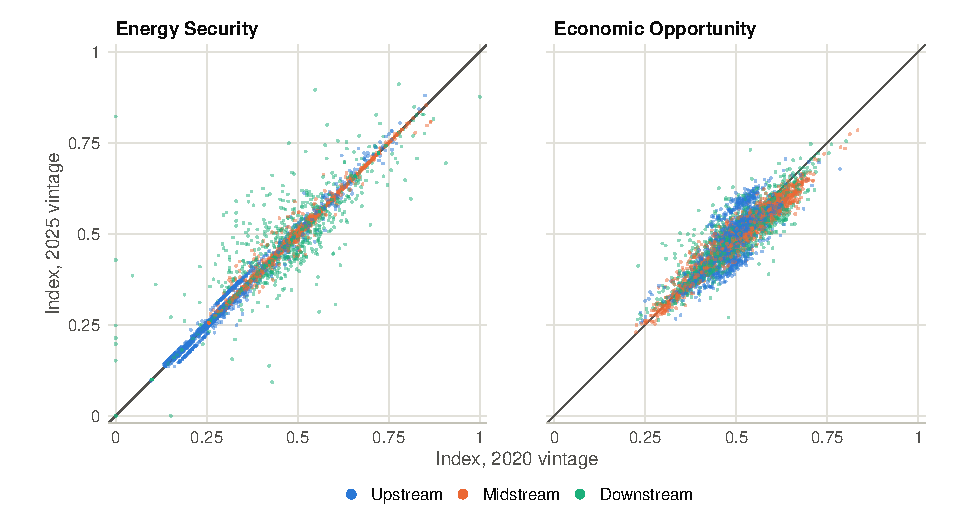
\includegraphics[width=\textwidth]{robustness_vintage}
  \caption{The 2020 and 2025 vintages of the pillars. Each point is a rankable country cell of the
  eleven headline technologies observed in both vintages (4{,}139 in $\ES$, 4{,}301 in $\EO$),
  coloured by stage; the line is the 45-degree line. Both vintages are built by
  \texttt{scripts/40\_build\_index\_vintages.R} with the headline builders and configuration; only
  the time-varying sources are sliced to the vintage year, and Trade is measured on the Atlas basis.
  Source: \texttt{data/processed/vintages}; \texttt{scripts/paper/fig\_robustness.R}.}
  \label{fig:robustness_vintage}
\end{figure}

\paragraph{Category weights.} The weight vectors are drawn as $w\sim\mathrm{Dir}(c\,\bar w)$ around
the configured shares $\bar w$, so that $E[w_k]=\bar w_k$ and the coefficient of variation of $w_k$
is $\sqrt{(1-\bar w_k)/[\bar w_k(c+1)]}$; $c=99$ for the ten categories of a pillar gives 0.3 for a
category of average weight \citep{decancq2013weights}. In seven $\ES$ pairs and three $\EO$ pairs a
single category varies, and there the ranking does not depend on the weights at all; on average 3
per cent of the observed weight of an $\ES$ pair and 25 per cent of an $\EO$ pair sits on categories
constant within it. Restricted to pairs with two or more varying categories (23 in $\ES$, 30 in
$\EO$), the median correlation over pair--draws is 0.996 and 0.987, but the minimum falls to 0.77
and 0.30. For each coalition member and pair, the 5th to 95th percentile band of its percentile
position over the draws has a median width of 2.8 points in $\ES$ (1{,}606 member cells) and 9.6 in
$\EO$ (1{,}718), with a 90th percentile of 18 and 31 points. Wide bands arise among large blocks of
tied scores: in $\ES$ Batteries Downstream South Korea ranks 69th of 186 at the configured weights
with a band from 15th to 186th; in $\EO$ the widest bands are Upstream, such as Brazil in Nuclear
Upstream (163rd of 175, band 21st to 174th). Figure~\ref{fig:robustness_ranks} shows one pair.

\begin{figure}[tbp]
  \centering
  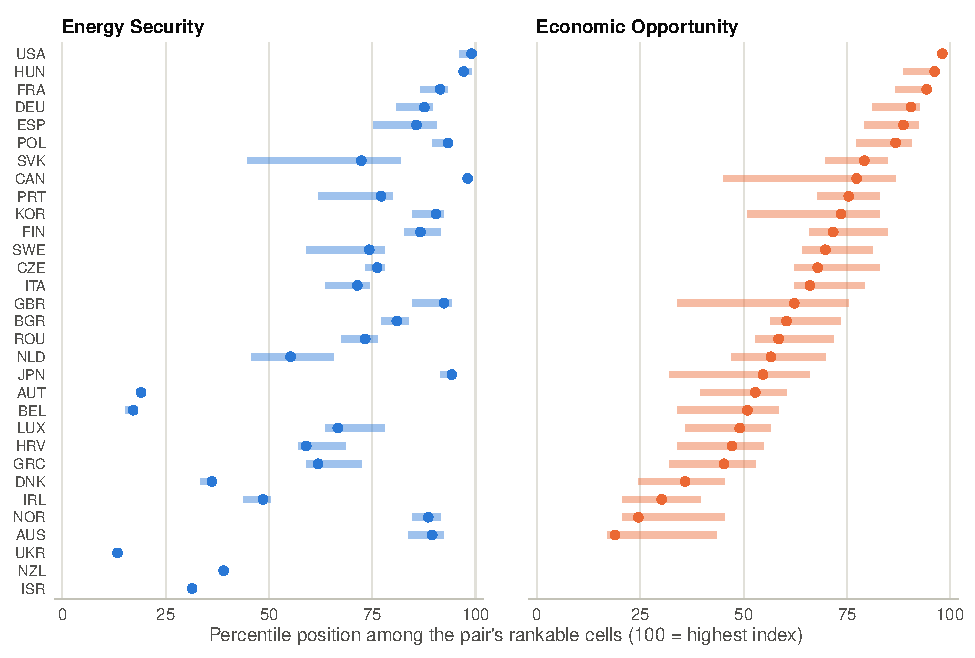
\includegraphics[width=\textwidth]{robustness_ranks}
  \caption{Rank uncertainty of the core members under perturbed category weights, Batteries
  Midstream. For each core member with a rankable cell (31 in $\ES$, 28 in $\EO$) the dot is its
  percentile position at the configured weights and the bar spans the 5th to 95th percentiles over
  1{,}000 Dirichlet draws (coefficient of variation 0.3 for a category of average weight). Source:
  category scores in \texttt{index\_outputs.rds}; \texttt{scripts/paper/fig\_robustness.R}.}
  \label{fig:robustness_ranks}
\end{figure}

\paragraph{Curvature.} Because $\operatorname{logit}\Scurve(r)=\gamma\operatorname{logit}r$, a
component at curvature $\gamma'$ follows from the stored value as
$\phi_{\gamma'}(r)=\operatorname{logistic}\big((\gamma'/0.5)\operatorname{logit}\phi_{0.5}(r)\big)$,
which also maps anchored zeros to zero. The map is exact for a component that is a single S-curve of
a rank; 46 of the 57 components that enter a scored category pass this test, carrying 84 per cent
of the average $\ES$ cell's weight and 63 per cent of the $\EO$ cell's. For the others (the input-
and levelised-cost terms, readiness, overcapacity, the production surplus of Energy Imports, the
mineral-supply and production shares of Foreign Dependency, the minerals-trade terms and the
geothermal and wind potential indices) it re-curves a mean and is an approximation. Levels move more
than ranks: the mean absolute change of $\ES$ is 0.03, 0.04 and 0.08 at $\gamma'=0.25$, 1 and 2.

\paragraph{Imputation.} Nine $\ES$ themes and twelve $\EO$ themes fill uncovered countries with the
observed mean of their component group (equation~\eqref{eq:impute}). Such components carry on average
7 per cent of an $\ES$ cell's weight, mainly in Energy Access and Foreign Dependency, and 25 per cent
of an $\EO$ cell's, two thirds of it in Technology Demand and most of the rest in Production and Cost
Competitiveness. The lowest within-pair correlations are Nuclear Upstream (0.62) without imputation
and Coal Downstream (0.58) with zeros in $\ES$, and Coal Midstream (0.29) without imputation in
$\EO$. Zero-filling places every uncovered economy at or below every covered one on the component;
removing the rule scores it on fewer measurements than its neighbours; the global average compresses
the differences the component would make. None is neutral.

\paragraph{Rankability.} Table~\ref{tab:robustness_rankability} varies $\tau$. Because the rule
filters cells without changing values, it changes the sample, not the order of cells rankable under
both thresholds. At $\tau=0.3$ the rankable cells are 56 per cent of the sovereign scored cells in
$\ES$ and 31 per cent in $\EO$ (74 and 67 per cent at the headline), at $\tau=0.7$ 95 and 93 per
cent. The median within-pair correlation of $\EO$ with its zero-filled variant is 0.94 at $\tau=0.3$,
0.77 at the headline and 0.68 at $\tau=0.7$. The top ten of 27 of the 30 $\ES$ pairs are identical at
$\tau=0.3$ but only 15 of the 33 $\EO$ top-ten lists. At $\tau=0.3$, 48 of the 57 members keep a pick
and 29 of them the baseline one; at $\tau=0.7$, 42 of 57 keep the baseline pick. At $\tau=0.3$ the
world view of the PSI ranks 102 partners and the core view 159.

% Generated by scripts/paper/fig_robustness.R; do not edit by hand.
\begin{table}[tbp]
  \centering
  \begin{threeparttable}
  \caption{The rankability threshold: cells ranked, robustness of their rankings, and the Strategic Index}
  \label{tab:robustness_rankability}
  \small
  \begin{tabular}{lcccccccccc}
    \toprule
    & \multicolumn{3}{c}{$\ES$} & \multicolumn{3}{c}{$\EO$} & \multicolumn{3}{c}{Strategic Index} & PSI \\
    \cmidrule(lr){2-4}\cmidrule(lr){5-7}\cmidrule(lr){8-10}\cmidrule(lr){11-11}
    $\tau$ & Cells & $\rho_{\text{none}}$ & $\rho_{\text{zero}}$ & Cells & $\rho_{\text{none}}$ & $\rho_{\text{zero}}$ & Cells & Countries & Picks & Ranked \\
    \midrule
    0.3 & 3{,}147 & 1.00 & 1.00 & 1{,}967 & 0.99 & 0.94 & 1{,}577 & 107 & 29/48 & 159/102 \\
    0.5$^{\ast}$ & 4{,}163 & 1.00 & 0.98 & 4{,}301 & 0.97 & 0.77 & 3{,}154 & 174 & 57/57 & 192/188 \\
    0.7 & 5{,}350 & 0.99 & 0.98 & 5{,}974 & 0.86 & 0.68 & 5{,}156 & 194 & 42/57 & 194/194 \\
    \bottomrule
  \end{tabular}
  \begin{tablenotes}[flushleft]\footnotesize
    \item \emph{Notes:} A cell is rankable when the economy is sovereign and at most a share $\tau$ of its index weight rests on imputed components ($^{\ast}$ the headline, \texttt{config/rankability.yml}). Cells: rankable headline cells (of 6{,}232 scored $\ES$ and 7{,}131 scored $\EO$ cells). $\rho_{\text{none}}$ and $\rho_{\text{zero}}$: median across technology--stage pairs of the within-pair Spearman correlation, over the cells rankable at $\tau$, between the baseline pillar and the pillar rebuilt with every global-average rule removed (available case) or replaced by zero. Strategic Index: cells and countries in the sample when the pillars' rankable flags are taken at $\tau$ (the Policy index is unchanged), and the number of coalition members whose allied pick is the baseline one, over the members with a pick at $\tau$. PSI: partners ranked in the core-coalition (headline) and world views. Within a technology--stage pair the order of two cells rankable under two thresholds is the same, because the rule filters cells and does not change values. Source: \texttt{scripts/paper/fig\_robustness.R} (\texttt{rankability} in \texttt{paper/results/robustness.json}).
  \end{tablenotes}
  \end{threeparttable}
\end{table}


\paragraph{Leave one category out and effective importance.} Figure~\ref{fig:robustness_loo} drops
one category at a time. In $\ES$ the ranking depends most on Consumption (median within-pair
correlation 0.74 over eight pairs) and Minerals Trade (0.79 over six); Trade has the widest range
(minimum 0.40 in Electric Grid Midstream, whose basket the completed trade file filled) and is the
only category of the four Midstream fossil and nuclear pairs. Production and Foreign Dependency,
which share the largest nominal $\ES$ weight, change almost nothing (0.995 and 0.998). In $\EO$,
Foreign Dependency (0.75), Cost Competitiveness (0.76) and Trade (0.79) carry most of the ranking,
while Technology Demand changes it little (0.99) and Technological Readiness and Energy Prices,
constant within pairs, not at all. A complementary, exact measure is the share of a pillar's
cross-country variance within a pair for which each category accounts. Because the pillar is the sum
of its category contributions $C_{kits}$ (equation~\eqref{eq:cat_decomp}),
\begin{equation}\label{eq:variance_share}
  S_{kts}=\frac{\operatorname{Cov}_i\bigl(C_{kits},\,\ES_{its}\bigr)}
               {\operatorname{Var}_i\bigl(\ES_{its}\bigr)},
  \qquad \sum_{k}S_{kts}=1,
\end{equation}
and likewise for $\EO$, a linear counterpart of the main effects of \citet{paruolo2013ratings}.
Table~\ref{tab:robustness_importance} compares nominal weights, mean effective weights and mean
variance shares. The share of weight that would have to move for nominal and variance shares to
coincide is 0.32 in $\ES$ and 0.37 in $\EO$. In $\ES$ the gap is mainly coverage: Trade, observed in
18 of the 30 pairs, has 9.5 per cent of the nominal weight but 24.9 per cent of the effective weight
and 21.5 per cent of the variance. In $\EO$ it arises within pairs: Technology Demand and
Technological Readiness hold 21.8 and 14.6 per cent of the effective weight but 3.6 and 0.0 per cent
of the variance, while Cost Competitiveness holds 21.9 and 32.8 per cent.

\begin{figure}[tbp]
  \centering
  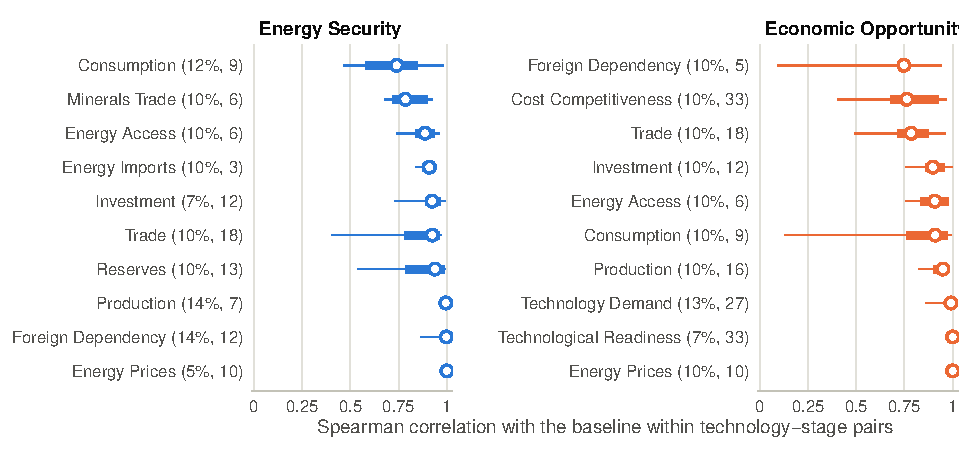
\includegraphics[width=\textwidth]{robustness_loo}
  \caption{Leave-one-category-out sensitivity of within-pair rankings: Spearman correlation between
  the baseline and the pillar without the category (remaining categories renormalised), over the
  pairs in which the category is observed and the baseline's rankable cells; open circle, median;
  thick bar, interquartile range; thin line, range. Labels give the nominal weight share and the
  number of pairs observed. Pairs in which the dropped category is the only varying one are omitted.
  Source: \texttt{index\_outputs.rds}; \texttt{scripts/paper/fig\_robustness.R}.}
  \label{fig:robustness_loo}
\end{figure}

% Generated by scripts/paper/fig_robustness.R; do not edit by hand.
\begin{table}[tbp]
  \centering
  \begin{threeparttable}
  \caption{Nominal weight, effective weight and variance share of each category within technology--stage pairs}
  \label{tab:robustness_importance}
  \small
  \begin{tabular}{lrrrrr}
    \toprule
    & Nominal & Effective & Variance & & Leave-one- \\
    Category & share (\%) & weight (\%) & share (\%) & Pairs & out $\rho$ \\
    \midrule
    \multicolumn{6}{l}{\emph{Panel A. Energy Security ($\ES$), 30 pairs}}\\
    \quad Trade & 9.5 & 24.9 & 21.5 & 18 & 0.93 \\
    \quad Investment & 7.1 & 11.3 & 18.1 & 12 & 0.92 \\
    \quad Reserves & 9.5 & 9.5 & 17.4 & 13 & 0.94 \\
    \quad Consumption & 11.9 & 15.8 & 13.2 & 9 & 0.74 \\
    \quad Foreign Dependency & 14.3 & 16.1 & 10.1 & 12 & 1.00 \\
    \quad Production & 14.3 & 5.8 & 10.0 & 7 & 0.99 \\
    \quad Energy Access & 9.5 & 7.2 & 5.0 & 6 & 0.89 \\
    \quad Energy Imports & 9.5 & 2.9 & 2.8 & 3 & 0.91 \\
    \quad Minerals Trade & 9.5 & 3.1 & 1.8 & 6 & 0.79 \\
    \quad Energy Prices & 4.8 & 3.4 & 0.0 & 10 & 1.00 \\
    \addlinespace
    \multicolumn{6}{l}{\emph{Panel B. Economic Opportunity ($\EO$), 33 pairs}}\\
    \quad Cost Competitiveness & 10.0 & 21.9 & 32.8 & 33 & 0.76 \\
    \quad Trade & 10.0 & 11.0 & 17.5 & 18 & 0.79 \\
    \quad Investment & 10.0 & 6.6 & 14.4 & 12 & 0.90 \\
    \quad Production & 10.0 & 8.1 & 12.5 & 16 & 0.95 \\
    \quad Consumption & 10.0 & 5.0 & 7.9 & 9 & 0.91 \\
    \quad Foreign Dependency & 10.0 & 2.9 & 7.4 & 5 & 0.75 \\
    \quad Energy Access & 10.0 & 2.8 & 3.8 & 6 & 0.91 \\
    \quad Technology Demand & 13.3 & 21.8 & 3.6 & 27 & 0.99 \\
    \quad Energy Prices & 10.0 & 5.3 & 0.0 & 10 & 1.00 \\
    \quad Technological Readiness & 6.7 & 14.6 & 0.0 & 33 & 1.00 \\
    \bottomrule
  \end{tabular}
  \begin{tablenotes}[flushleft]\footnotesize
    \item \emph{Notes:} Nominal share: $w_k/\sum_{k'}w_{k'}$ from \texttt{config/weights.yml}. Effective weight: mean over the rankable headline pairs of the weight $w_k/\sum_{l\ \mathrm{observed}}w_l$ a category receives after renormalisation over the observed categories; zero where the category is not observed. Variance share: mean over the same pairs of $S_{kts}$ (equation~\eqref{eq:variance_share}), the covariance of the category's contribution with the pillar across the rankable cells of the pair divided by the pillar's variance; zero where the category is not observed. Each of the three columns sums to 100 within a panel up to rounding. Pairs: number of pairs in which the category is observed. Leave-one-out $\rho$: median, over the pairs in which the category is observed and the reduced pillar still ranks countries, of the within-pair Spearman correlation between the baseline pillar and the pillar without the category (Figure~\ref{fig:robustness_loo}). Rows are ordered by the variance share. Sample: rankable cells of the eleven headline technologies. Source: category scores in \texttt{index\_outputs.rds}; \texttt{scripts/paper/fig\_robustness.R} (\texttt{weights.<pillar>.variance\_importance} in \texttt{paper/results/robustness.json}).
  \end{tablenotes}
  \end{threeparttable}
\end{table}


\paragraph{Strategic Index weights and policy variants.} The Dirichlet draws of the five weights of
equation~\eqref{eq:si} use concentration 43.4, giving coefficients of variation of 0.30 for the
policy weight, 0.23 for the two pillar weights and 0.45 for the two priors. Indonesia keeps its pick
in 15 per cent of the draws, its two leading sectors differing by 0.0007. Under security in place of
need, 28 members pick Nuclear Midstream and 10 Gas Midstream; without the priors, ten picks move to
Oil Midstream, the sector the technology prior penalises most; without the policy term, 20 members
pick Nuclear Upstream instead of 8. Requiring both Policy components leaves 1{,}666 Strategic Index
cells; dropping CAT for every country gives a median within-country Strategic Index correlation of
1.00 (interquartile range 0.91 to 1.00, minimum 0.30). The October 2026 NIPO component (GTA NIPO as of
5 October 2026, debiased strength; 1{,}070 rows), added with weights 4, 3 and 2 on NIPO, IEA PAMS and
CAT and IEA PAMS still required, is observed in Upstream and Midstream cells only, in 841 Strategic
Index cells (27 per cent); for its jurisdictions the within-country Spearman correlation between the
policy ranks with and without it has a median of 0.88 (range 0.00 to 1.00), the pooled Strategic
Index correlation is 0.97, and 27 of the 50 members with a NIPO score keep their pick.

\paragraph{Data choices of the final build.} Table~\ref{tab:robustness_data} and
Figure~\ref{fig:robustness_picks_data} report the data choices of the last revision (11--12 October
2026). The headline carries 807 EIA-sourced rows in the import-dependence theme and 656 in the
production theme; setting them to zero gives within-pair correlations of 0.97 to 0.98 in $\ES$ and
0.95 to 0.96 in $\EO$ in Oil, Gas and Coal Upstream. Removing Trade from the four Upstream cells with
new baskets gives median within-pair correlations of 0.94 in $\ES$ and 0.73 in $\EO$ (minimum 0.58,
Solar Upstream $\EO$) and returns the Strategic Index to 192 countries, because the newly imputed
Trade category had pushed small economies over the rankability threshold; three of the four changed
picks move to Nuclear Upstream. The superseded energy-trade file is not kept, but interim builds
record the picks: on 8 October, 45 of the 56 members then in the coalition had a pick, 17 Electric
Grid Midstream and 11 Batteries Midstream; on 10 October, 4 and 26 of 57. Without Trade, Electric
Grid Midstream picks rise to 10 and Batteries Midstream falls to 13; without Technological Readiness
32 of 57 picks survive (Electric Grid Midstream would take 27), without Technology Demand 41 and
without Foreign Dependency 44. The CM-FDI comparison is not re-run on the final outputs, because the
dyad tables exceed the memory budget of the replication; in the integration study, switching off the
Chinese-parent component or the CM-FDI investment ties alone gives core-PSI correlations of 0.9999.

\begin{figure}[tbp]
  \centering
  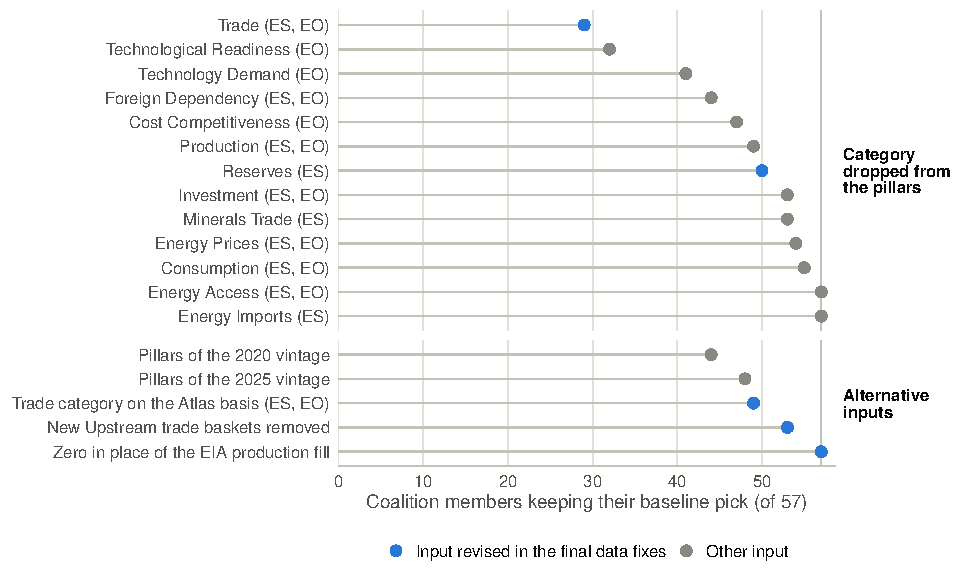
\includegraphics[width=\textwidth]{robustness_picks_data}
  \caption{Stability of the allied picks under the data inputs: number of members, of 57, whose pick
  is the baseline one when the Strategic Index takes pillars rebuilt under a variant. Upper panel:
  one category dropped (without Trade three members have no eligible rankable sector, so 29 of the
  54 with a pick keep it). Lower panel: pillars from the 2020 or 2025 vintage, Trade on the Atlas
  basis, Trade removed from the four Upstream cells whose baskets were added on 11 October 2026, and
  EIA-filled fossil production set to zero. Blue marks inputs revised in the final data fixes. The
  Policy index and the endowment screen are the headline ones. Source: \texttt{index\_outputs.rds},
  theme tables, vintages; \texttt{scripts/paper/fig\_robustness.R}.}
  \label{fig:robustness_picks_data}
\end{figure}

% Generated by scripts/paper/fig_robustness.R; do not edit by hand.
\begin{table}[tbp]
  \centering
  \begin{threeparttable}
  \caption{Data and policy choices of the final build: rankable cells, rankings and allied picks}
  \label{tab:robustness_data}
  \footnotesize
  \setlength{\tabcolsep}{4pt}
  \begin{tabular}{lccccccc}
    \toprule
    & \multicolumn{2}{c}{Rankable cells} & \multicolumn{2}{c}{Median $\rho$, touched pairs} & \multicolumn{3}{c}{Strategic Index} \\
    \cmidrule(lr){2-3}\cmidrule(lr){4-5}\cmidrule(lr){6-8}
    Variant & $\ES$ & $\EO$ & $\ES$ & $\EO$ & Cells & Countries & Same pick \\
    \midrule
    Baseline & 4{,}163 & 4{,}301 & -- & -- & 3{,}154 & 174 & 57/57 \\
    \multicolumn{8}{l}{\emph{Data}}\\
    \quad Zero in place of the EIA fill & 4{,}164 & 4{,}301 & 0.98 & 0.96 & 3{,}155 & 174 & 57/57 \\
    \quad New Upstream baskets removed & 4{,}161 & 4{,}307 & 0.94 & 0.73 & 3{,}144 & 192 & 53/57 \\
    \multicolumn{8}{l}{\emph{Policy index}}\\
    \quad Both components required & = & = & -- & -- & 1{,}666 & 65 & 46/46 \\
    \quad IEA PAMS alone & = & = & -- & -- & 3{,}154 & 174 & 45/57 \\
    \quad October 2026 NIPO added back & = & = & -- & -- & 3{,}154 & 174 & 34/57 \\
    \multicolumn{8}{l}{\emph{Allied pick rule}}\\
    \quad Endowment screen off & = & = & -- & -- & 3{,}154 & 174 & 16/57 \\
    \bottomrule
  \end{tabular}
  \begin{tablenotes}[flushleft]\footnotesize
    \item \emph{Notes:} Rankable cells: headline cells of sovereign economies with at most half of the index weight imputed, after the variant (= unchanged). Median $\rho$: median across the touched technology--stage pairs (Oil, Gas and Coal Upstream for the EIA fill; Electric Vehicles, Wind, Nuclear and Solar Upstream for the baskets) of the within-pair Spearman correlation between the baseline and the variant over the baseline's rankable cells. Strategic Index: scored cells and countries, and the coalition members whose allied pick is the baseline one over the members with a pick. Zero in place of the EIA fill: the oil, gas and coal production that the Energy Institute does not report (807 EIA-sourced rows of the import-dependence theme and 656 of the production theme in the headline) set to zero, the rule until 11 October 2026, both themes rebuilt with the pipeline's builders. New Upstream baskets removed: the Trade category of the four Upstream cells whose trade baskets were added on 11 October 2026 dropped and both pillars rebuilt; the uranium codes moved out of Nuclear Midstream and the rare-earth codes moved out of EV and Wind Midstream are not restored. Policy rows as in Table~\ref{tab:robustness_picks}. The partnership side is not rebuilt: in the CM-FDI integration study (inputs of 11 October 2026), switching off both CM-FDI parts of Friendshore gives a core-view PSI with a Spearman correlation of 0.9998 with the CM-FDI build over 192 ranked partners, a largest rank change of 5 places and 15 of the top 15 in common. Source: \texttt{scripts/paper/fig\_robustness.R} (\texttt{data\_choices} and \texttt{policy} in \texttt{paper/results/robustness.json}).
  \end{tablenotes}
  \end{threeparttable}
\end{table}


\paragraph{Vertical complementarities.} The opportunity test regresses the five-year change in a
stage's S-curved world market share, and entry into revealed comparative advantage, on the adjacent
stage's market-share index, with country--year and technology--year fixed effects and standard
errors clustered by country. The cross-sectional association is positive and precisely estimated
(0.046, standard error 0.007, for Midstream on Upstream; 0.102, standard error 0.015, for the
reverse) but concentrated in fossil fuels and nuclear (0.062 and 0.151) and insignificant for the
clean-technology chains (0.012 and 0.028); with country--technology fixed effects it is $-0.001$
(0.005) and 0.004 (0.015); lags of the stage's own capability absorb about a third of it; and it does
not improve out-of-sample prediction (within-cell AUC for Midstream entry 0.800 without the term and
0.794 with it; 0.739 and 0.741 for Upstream). The 2023 co-location lift, the ratio of the joint to
the independent probability of comparative advantage in both stages, is 4.4 for nuclear and 2.7 for
coal but 0.97 for wind and below one for gas, electric vehicles and the grid. The security test builds
the domestic share times the economy's own supply security plus the import-share-weighted security of
its suppliers (half the supplier's $\ES$ in the input stage, half dyadic alignment). Its 2020 value
does not predict import shortfalls in 2021--22 (0.10, standard error 0.31) or Midstream export
growth after 2020 (0.02, standard error 0.19), whereas sourcing concentration does (negative,
$p=0.035$); the post-2022 shift of Upstream input trade towards aligned suppliers, 0.58 log points
(0.11), falls to 0.07 (0.06) without Russia. Table~\ref{tab:robustness_vertical} reports what the two
terms would do at the evidence weights. The $\EO$ term, the adjacent stage's S-curved Atlas share
minus the economy's mean of that measure over the nine basketed technologies, S-curved within the
cell, enters with 0.07 weight points in Midstream and 0.23 in Upstream (0.6 and 1.5 per cent of a
cell's mean observed weight): median within-pair correlation 0.999 (minimum 0.987), one pick changed
(Luxembourg's, the smallest margin in the coalition), against 0 to 1 for a placebo with scores
permuted within cells. The $\ES$ term at a 15 per cent share gives median correlations of 0.92 in
Midstream and 0.91 in Downstream (minimum 0.56, Batteries Downstream) and changes 10 picks, against
11 (8 to 16) for the permuted placebo and 3 for a constant placebo that only rescales the other
categories.

% Generated by scripts/paper/fig_robustness.R; do not edit by hand.
\begin{table}[tbp]
  \centering
  \begin{threeparttable}
  \caption{Vertical complementarities: sensitivity of the pillars and the allied picks to an adjacent-stage term}
  \label{tab:robustness_vertical}
  \footnotesize
  \setlength{\tabcolsep}{4pt}
  \begin{tabular}{llccc}
    \toprule
    Term & Weight & \makecell{Median within-\\pair $\rho$} & \makecell{Minimum\\$\rho$} & \makecell{Picks\\changed} \\
    \midrule
    $\EO$ linkage, within-country deviation & Mid 0.07, Up 0.23 & 0.999 & 0.987 & 1 \\
    \quad Placebo: scores permuted within cell & same & 0.999 [0.999, 0.999] & -- & 0 [0, 1] \\
    \addlinespace
    $\ES$ input security, sourcing-weighted & 15\% share & 0.917 & 0.556 & 10 \\
    \quad Placebo: constant 0.5 & same & 1.000 & 1.000 & 3 \\
    \quad Placebo: scores permuted within cell & same & 0.902 [0.891, 0.909] & -- & 11 [8, 16] \\
    \bottomrule
  \end{tabular}
  \begin{tablenotes}[flushleft]\footnotesize
    \item \emph{Notes:} $\EO$ linkage: a category added to the Midstream and Upstream $\EO$ cells, the S-curved world market share of the adjacent stage (Atlas of Economic Complexity, HS92 baskets, 2023) minus the economy's mean of that measure over the 9 basketed headline technologies, S-curved within the cell (Midstream 1{,}890; Upstream 1{,}890 cells). Weights in $\EO$ weight points (the nominal category weights are 2 to 4): the evidence weights of the vertical-complementarity study, 0.6 times the ratio of the adjacent-stage to the feasibility coefficient in the five-year market-share regression, upper bounds because about a third of the coefficient is absorbed by lags of own capability. $\ES$ input security: the domestic supply share times the economy's own supply security plus the import-share-weighted security of its suppliers (half the supplier's $\ES$ in the input stage, half the dyadic alignment), 2024 sourcing, S-curved within the cell and given 15 per cent of the Midstream and Downstream cells' weight (Downstream 1{,}626; Midstream 1{,}893 cells). Median and minimum $\rho$: within-pair Spearman correlation with the baseline pillar over the baseline's rankable cells of the receiving stages; for the permutation placebo, the median and the 5th and 95th percentiles over 200 draws of the per-draw median. Picks changed: coalition members (of 57) whose allied pick differs from the baseline when the Strategic Index takes the modified pillar (for the placebo, median and 5th--95th percentiles over the draws). Neither term enters the headline indices. Source: \texttt{scripts/paper/fig\_robustness.R} (\texttt{vertical} in \texttt{paper/results/robustness.json}), from the study's inputs.
  \end{tablenotes}
  \end{threeparttable}
\end{table}


% Online Appendix to Appendix D (app:corrections). Item-level detail of the corrections listed in
% Table tab:corrections_index: defect, symptom in the shipped release, correction, and the
% pre-rerun effect measured by the audit on the shipped inputs (not a result of the paper).
% Sources: the audit's fix logs and reviews, git log of branch fix/allied-base-paper, README
% changelog, and the corrected code in R/, scripts/, config/.
\section{Corrections to the shipped release: item detail}\label{oa:corrections}

This appendix gives, for each item of Table~\ref{tab:corrections_index}, the defect, its symptom in
the shipped release of September 2026, the correction and, where the audit measured it, the
\emph{pre-rerun effect}: the change the correction makes when applied alone to the theme tables and
inputs saved with the shipped release. Pre-rerun effects isolate one correction on inputs that
still embed the other defects; they are not results of the paper.

\paragraph{Aggregation (A1--A7).} A1: an unobserved category kept its weight in the denominator and
counted as zero, and a cell with no observed category scored zero; 1{,}809 of 2{,}773 headline ES
Reserves rows were unobserved. The available-case rule alone changes 1{,}682 Upstream cells and
raises mean Upstream ES by 0.139 (Oil), 0.112 (Gas) and 0.104 (Coal). Because the same commit gives
Reserves a zero rule (the reserve tables list every material holder, so absence means none), the two
changes offset on the shipped tables; the rule matters for categories without a missing-data rule
and for the PSI (B4). A2: a zero or global-average rule filled groups in which no country was
observed; it now fills only groups with an observed country and reports the rest. A3:
\texttt{any(isTRUE(x))} is \texttt{FALSE} for vectors longer than one, so the diagnostics reported
11.9 and 29.5 percent of ES and EO category scores as imputed against 37.0 and 69.2 percent in fact;
the final run has 38.4 and 45.0 percent. A4: Energy Prices was configured on a variable no theme
produced and dropped from both pillars without warning, because the guard compared the join keys with
themselves; it re-enters ten Upstream cells as a world price series that shifts cell levels and
leaves within-cell order unchanged (Spearman 1.000 in every varying cell). A second guard now warns
when a theme's own composite is scored in place of a configured overall. A5: an EO Reserves weight
of 2 for a category EO does not have let resource-potential rows create 88 fully imputed EO cells
(the Holy See, the Pitcairn Islands); EO falls from 6{,}923 to 6{,}835 headline cells. A6: the
variable-contribution table divided by the number of components including missing ones; both
decompositions now reconcile to the index (largest error $1.1\times10^{-16}$). A7: a development
commit made \texttt{bind\_rows()} read a named list of tables as one row; a rerun from that revision
would have removed every overall-based category.

\paragraph{Country universe (C1--C3).} C1: the standardiser attached ISO3 codes but did not rename
rows, so the shipped ES, EO, Strategic and Policy tables carried 272 strings for 237 economies, with
30 codes under two or three spellings (Viet Nam and Vietnam, Korea and South Korea, the two Congos).
Each spelling took its own rank in every S-curve with a partly observed, often imputed profile.
Every variant now maps to the WDI name of its code \citep{worldbank2026wdi}; territories with their
own code stay separate. C2: the EI ``USSR'' series, a CIS aggregate, was coded RUS, ``Northern
Cyprus'' CYP, and a pseudo-country ``Global'' carried readiness values (128 rows); aggregates,
residuals and historical entities are now dropped, not merged into successors. C3: the 2025
critical-minerals Comtrade pulls hold three reporters against about 130 in 2024; a vintage needs 50.

\paragraph{Energy Security themes (E1--E12).} E1: graphite and rare earths fell out of every join
because the IEA and EI name them differently; with harmonised names the rare earths carry about 79
percent of Wind's Mineral Supply weight. E2: the stage recode mapped refining to the Upstream under
both branches; refining now scores the Midstream. E3: listed non-producers (Germany, Japan) tied at
0.441 just below the Congo at 0.473 in Batteries Upstream while unlisted economies scored zero; zero
supply now maps to zero for every economy and suppliers rank above it. E4: the reserves roll-up
averaged only over listed minerals, so Chile scored 1.000 on Wind Reserves on copper alone. E5: BNEF
onshore and offshore wind were never recoded, so Wind had no Consumption category; growth was ranked
across technologies; Viet Nam's rows fall from 160 to 63 once each country receives one regional
value. E6: Minerals Trade kept only the market-share index; it is now the mean of a demand-weighted
market share and a concentration index $\Scurve(-\HHI_m)$. E7: critical-minerals investment was
copied in full to Batteries and EV Upstream (79.8 each; now 9.2 and 70.6), and stage completion
manufactured zero Investment cells in Nuclear Upstream and Midstream and Geothermal Upstream and
Midstream, which made those cells constant across countries and gave Nuclear Upstream the maximum
security need for every country. E8: electrolyser capacity was filed outside the headline
technologies. E9: mineral Upstream production depth was an unweighted mean of different minerals'
kilotonnes; it is now a demand-weighted share of world mined supply, with growth as an absolute
change (EO moves by up to 0.067 in six cells, within-cell Spearman 0.955--0.992). E10: a placeholder
region dropped the eight non-EU European EI economies from EV Midstream. E11: the EI ``Import
share'' (a self-sufficiency ratio) and the EV ``import\_share'' (a net-export ratio) are renamed for
what they measure, and non-producers now tie exactly in Energy Imports. E12: an economy without its
own EI production row (EI counts it in a regional residual) was read as producing nothing, so New
Zealand counted as importing all its gas; production then comes from EIA International Energy
Statistics \citep{eia2026international}, flagged and counted as observed, paired with consumption of
the same year (Estonia coal stays missing because EI counts oil shale). On the inputs of 10 October
2026 this moves 605 ES Upstream fossil cells and no allied pick.

\paragraph{Trade and Economic Opportunity (T1--T13).} T1: the ES and EO trade themes were identical
tables and the ES deficit term was never computed; ES Trade is now concentration, basket share and
net basket imports over GDP, EO Trade share, RCA \citep{balassa1965trade}, export size, feasibility
and concentration (earlier--corrected Spearman 0.54--0.91 across cells). T2: export size and
feasibility were ranked within reporter, so Moldova and Samoa ranked beside China in Solar
Midstream. T3: market share was the export-weighted mean of product-level world shares; the Congo
had 0.862 against a basket share of 0.0074 in Batteries Midstream. T4: ores, slag and scrap were
filed under Batteries Midstream, untreated softwood logs under three grid and renewable baskets, and
16 keys appeared twice. T5: 73 crosswalk codes had no HS92 counterpart, so the Atlas EV Midstream
basket contained no cars; 19 predecessor codes bridge them. T6: the levelised cost entered Cost
Competitiveness four times (0.78 of the category's weight where quoted). T7: readiness was written for
a pseudo-country and reached real economies only by imputation. T8: Technology Demand listed
composites beside their own sub-indices and ranked a zero addressable market as the smallest. T9: the
export-concentration index was ranked across every basket, so unscored baskets (Semiconductors)
moved scored cells; it is now ranked over the headline cells. T10: the Comtrade energy-trade file
lacked 60 basket codes and 13 reporters, among them Qatar's LNG (USD 56.9bn in 2024); it is rebuilt
from the World rows of the all-reporter dyad pull. T11--T13: duplicate WEO and BNEF demand keys,
IEA 2035 manufacturing shares taken without the ``Other'' row (China's 2035 solar share 0.90 rather
than 0.80), zero lending-rate stubs (New Zealand 0.0 percent, now 4.76) and mislabelled IMF price
units \citep{imf2026pcps}; only the lending rates move an index value.

\paragraph{Policy and Strategic indices (P1--P9).} P1: the NIPO module's jurisdiction weights
overwrote the IEA module's, so international IEA policies were weighted 0.20 instead of 0.66. P2:
Upstream stage tags matched substrings (``ore'' in ``more'', ``Korea'', ``Singapore''), tagging 36.9
percent of IEA policies Upstream; whole-word rules tag 12.5 percent. P3: name mismatches left South
Korea, the United Arab Emirates (coded ``UAE''), France, Italy and Denmark without a Policy index;
EU members without a national CAT rating now take the EU's \citep{cat2026ratings}. P4: the policy
block had stopped before writing its table since 6~February 2026, so the September Strategic Index
combined September pillars with February policy components. P5: NIPO's default as-of date was the
latest announcement or implementation date (1~October 2028 in every 2026 extract), counting
scheduled measures as in force; it is now the extract's last announcement, capped at the release
month and run date. NIPO is no longer in the composite; the robustness variant uses the October 2026
extract as of 5~October 2026. P6: the strategic table overwrote the security column with $1-\ES$; it
now carries security and need under their own names (no value changes). P7: missing pillar or policy
values were filled with country means (51 of 571 shipped cells); a cell now needs all three. P8:
sectors with a constant pillar were not detected; Nuclear Upstream, constant at zero, was the top
pick of 8 of 18 shipped allies. P9: the staged oil lifecycle emissions (720 g CO$_2$eq/kWh) appear in
no IPCC table; the SRREN median of 840 \citep{moomaw2011annex} replaces it next to the AR5 values of
the other technologies \citep{schlomer2014annex}, so the oil weight falls from 0.12 to 0 and coal's
rises from 0 to 0.02.

\paragraph{Bilateral indices (B1--B5).} B1: grouped \texttt{transmute()} calls, name keys and a
self-crossed backbone duplicated the Friendshore table (17.5 million rows for 1.44 million cells),
so a dyad's best-five mean weighted its top cells 2, 2 and 1. B2: \texttt{mean(a:b)} returned
\texttt{a}, so outward investment was the rank of the level only; 99 of 259 IMF counterpart names did
not match, so China and the Netherlands scored zero from every reporter. B3: development potential,
a partner-level construct, was stored per reporter with donor fan-out up to 38 rows, with 56
aggregates and mis-oriented WDI series. B4: a high-income partner's undefined development score kept
its weight, capping its PSI at 0.8 and placing the United States 185th of 218. B5: an opportunity
column named for security held the partner's need, and the tables covered 18 to 20 pseudo-technologies
rather than the eleven headline ones.

\paragraph{Network (N1--N7).} These defects concerned the network design that the paper no longer
uses; Appendix~\ref{app:corrections} records them, with the design itself, in one paragraph.


\end{document}
